\documentclass[twoside]{book}

% Packages required by doxygen
\usepackage{fixltx2e}
\usepackage{calc}
\usepackage{doxygen}
\usepackage[export]{adjustbox} % also loads graphicx
\usepackage{graphicx}
\usepackage[utf8]{inputenc}
\usepackage{makeidx}
\usepackage{multicol}
\usepackage{multirow}
\PassOptionsToPackage{warn}{textcomp}
\usepackage{textcomp}
\usepackage[nointegrals]{wasysym}
\usepackage[table]{xcolor}

% NLS support packages
\usepackage{hfont}

% Font selection
\usepackage[T1]{fontenc}
\usepackage[scaled=.90]{helvet}
\usepackage{courier}
\usepackage{amssymb}
\usepackage{sectsty}
\renewcommand{\familydefault}{\sfdefault}
\allsectionsfont{%
  \fontseries{bc}\selectfont%
  \color{darkgray}%
}
\renewcommand{\DoxyLabelFont}{%
  \fontseries{bc}\selectfont%
  \color{darkgray}%
}
\newcommand{\+}{\discretionary{\mbox{\scriptsize$\hookleftarrow$}}{}{}}

% Page & text layout
\usepackage{geometry}
\geometry{%
  a4paper,%
  top=2.5cm,%
  bottom=2.5cm,%
  left=2.5cm,%
  right=2.5cm%
}
\tolerance=750
\hfuzz=15pt
\hbadness=750
\setlength{\emergencystretch}{15pt}
\setlength{\parindent}{0cm}
\setlength{\parskip}{3ex plus 2ex minus 2ex}
\makeatletter
\renewcommand{\paragraph}{%
  \@startsection{paragraph}{4}{0ex}{-1.0ex}{1.0ex}{%
    \normalfont\normalsize\bfseries\SS@parafont%
  }%
}
\renewcommand{\subparagraph}{%
  \@startsection{subparagraph}{5}{0ex}{-1.0ex}{1.0ex}{%
    \normalfont\normalsize\bfseries\SS@subparafont%
  }%
}
\makeatother

% Headers & footers
\usepackage{fancyhdr}
\pagestyle{fancyplain}
\fancyhead[LE]{\fancyplain{}{\bfseries\thepage}}
\fancyhead[CE]{\fancyplain{}{}}
\fancyhead[RE]{\fancyplain{}{\bfseries\leftmark}}
\fancyhead[LO]{\fancyplain{}{\bfseries\rightmark}}
\fancyhead[CO]{\fancyplain{}{}}
\fancyhead[RO]{\fancyplain{}{\bfseries\thepage}}
\fancyfoot[LE]{\fancyplain{}{}}
\fancyfoot[CE]{\fancyplain{}{}}
\fancyfoot[RE]{\fancyplain{}{\bfseries\scriptsize 다음에 의해 생성됨 \+:  Doxygen }}
\fancyfoot[LO]{\fancyplain{}{\bfseries\scriptsize 다음에 의해 생성됨 \+:  Doxygen }}
\fancyfoot[CO]{\fancyplain{}{}}
\fancyfoot[RO]{\fancyplain{}{}}
\renewcommand{\footrulewidth}{0.4pt}
\renewcommand{\chaptermark}[1]{%
  \markboth{#1}{}%
}
\renewcommand{\sectionmark}[1]{%
  \markright{\thesection\ #1}%
}

% Indices & bibliography
\usepackage{natbib}
\usepackage[titles]{tocloft}
\setcounter{tocdepth}{3}
\setcounter{secnumdepth}{5}
\makeindex

% Hyperlinks (required, but should be loaded last)
\usepackage{ifpdf}
\ifpdf
  \usepackage[pdftex,pagebackref=true]{hyperref}
\else
  \usepackage[ps2pdf,pagebackref=true]{hyperref}
\fi
\hypersetup{%
  colorlinks=true,%
  linkcolor=blue,%
  citecolor=blue,%
  unicode%
}

% Custom commands
\newcommand{\clearemptydoublepage}{%
  \newpage{\pagestyle{empty}\cleardoublepage}%
}

\usepackage{caption}
\captionsetup{labelsep=space,justification=centering,font={bf},singlelinecheck=off,skip=4pt,position=top}

%===== C O N T E N T S =====

\begin{document}

% Titlepage & ToC
\hypersetup{pageanchor=false,
             bookmarksnumbered=true,
             pdfencoding=unicode
            }
\pagenumbering{roman}
\begin{titlepage}
\vspace*{7cm}
\begin{center}%
{\Large M\+C\+N\+Tactics \\[1ex]\large 1.\+0.\+0 }\\
\vspace*{1cm}
{\large 다음에 의해 생성됨 \+:  Doxygen 1.8.11}\\
\end{center}
\end{titlepage}
\clearemptydoublepage
\tableofcontents
\clearemptydoublepage
\pagenumbering{arabic}
\hypersetup{pageanchor=true}

%--- Begin generated contents ---
\chapter{네임스페이스 색인}
\section{패키지}
다음은 패키지들입니다. (가능한한 간략한 설명만을 보여줍니다) \+:\begin{DoxyCompactList}
\item\contentsline{section}{\hyperlink{namespace_m_c_n}{M\+CN} }{\pageref{namespace_m_c_n}}{}
\end{DoxyCompactList}

\chapter{계통도 색인}
\section{클래스 계통도}
이 상속 목록은 완전하진 않지만 알파벳순으로 대략적으로 정렬되어있습니다.\+:\begin{DoxyCompactList}
\item I\+Disposable\begin{DoxyCompactList}
\item \contentsline{section}{M\+C\+N.\+State}{\pageref{class_m_c_n_1_1_state}}{}
\begin{DoxyCompactList}
\item \contentsline{section}{Moveable\+Object.\+Moveable\+State}{\pageref{class_moveable_object_1_1_moveable_state}}{}
\begin{DoxyCompactList}
\item \contentsline{section}{Moveable\+Object.\+Moveable\+State\+\_\+\+Move}{\pageref{class_moveable_object_1_1_moveable_state___move}}{}
\item \contentsline{section}{Moveable\+Object.\+Moveable\+State\+\_\+\+Normal}{\pageref{class_moveable_object_1_1_moveable_state___normal}}{}
\end{DoxyCompactList}
\item \contentsline{section}{Tile.\+Tile\+State}{\pageref{class_tile_1_1_tile_state}}{}
\begin{DoxyCompactList}
\item \contentsline{section}{Tile.\+Tile\+State\+\_\+\+Active}{\pageref{class_tile_1_1_tile_state___active}}{}
\item \contentsline{section}{Tile.\+Tile\+State\+\_\+\+Deactive}{\pageref{class_tile_1_1_tile_state___deactive}}{}
\item \contentsline{section}{Tile.\+Tile\+State\+\_\+\+Normal}{\pageref{class_tile_1_1_tile_state___normal}}{}
\end{DoxyCompactList}
\end{DoxyCompactList}
\item \contentsline{section}{Placeable\+Object}{\pageref{class_placeable_object}}{}
\begin{DoxyCompactList}
\item \contentsline{section}{Moveable\+Object}{\pageref{class_moveable_object}}{}
\end{DoxyCompactList}
\item \contentsline{section}{Tile}{\pageref{class_tile}}{}
\end{DoxyCompactList}
\item \contentsline{section}{M\+C\+N.\+I\+Observable$<$ T $>$}{\pageref{interface_m_c_n_1_1_i_observable}}{}
\item \contentsline{section}{M\+C\+N.\+I\+Observable$<$ e\+Touch\+Event $>$}{\pageref{interface_m_c_n_1_1_i_observable}}{}
\begin{DoxyCompactList}
\item \contentsline{section}{Touch\+Manager}{\pageref{class_touch_manager}}{}
\end{DoxyCompactList}
\item \contentsline{section}{M\+C\+N.\+I\+Observer$<$ T $>$}{\pageref{interface_m_c_n_1_1_i_observer}}{}
\item \contentsline{section}{M\+C\+N.\+I\+Observer$<$ e\+Touch\+Event $>$}{\pageref{interface_m_c_n_1_1_i_observer}}{}
\begin{DoxyCompactList}
\item \contentsline{section}{Moveable\+Object}{\pageref{class_moveable_object}}{}
\item \contentsline{section}{Tile}{\pageref{class_tile}}{}
\end{DoxyCompactList}
\item \contentsline{section}{I\+Tile\+Active}{\pageref{interface_i_tile_active}}{}
\begin{DoxyCompactList}
\item \contentsline{section}{Placeable\+Object}{\pageref{class_placeable_object}}{}
\end{DoxyCompactList}
\item \contentsline{section}{Map\+Creator}{\pageref{class_map_creator}}{}
\item Mono\+Behaviour\begin{DoxyCompactList}
\item \contentsline{section}{M\+C\+N.\+Mono\+Singletone$<$ T $>$}{\pageref{class_m_c_n_1_1_mono_singletone}}{}
\item \contentsline{section}{Tactics\+Object}{\pageref{class_tactics_object}}{}
\begin{DoxyCompactList}
\item \contentsline{section}{Placeable\+Object}{\pageref{class_placeable_object}}{}
\item \contentsline{section}{Tile}{\pageref{class_tile}}{}
\end{DoxyCompactList}
\end{DoxyCompactList}
\item \contentsline{section}{M\+C\+N.\+Mono\+Singletone$<$ Map\+Manager $>$}{\pageref{class_m_c_n_1_1_mono_singletone}}{}
\begin{DoxyCompactList}
\item \contentsline{section}{Map\+Manager}{\pageref{class_map_manager}}{}
\end{DoxyCompactList}
\item \contentsline{section}{M\+C\+N.\+Mono\+Singletone$<$ Touch\+Manager $>$}{\pageref{class_m_c_n_1_1_mono_singletone}}{}
\begin{DoxyCompactList}
\item \contentsline{section}{Touch\+Manager}{\pageref{class_touch_manager}}{}
\end{DoxyCompactList}
\item \contentsline{section}{Map\+Manager.\+Place\+Info}{\pageref{class_map_manager_1_1_place_info}}{}
\item \contentsline{section}{M\+C\+N.\+Singletone$<$ T $>$}{\pageref{class_m_c_n_1_1_singletone}}{}
\item \contentsline{section}{M\+C\+N.\+Singletone$<$ Game\+Manager $>$}{\pageref{class_m_c_n_1_1_singletone}}{}
\begin{DoxyCompactList}
\item \contentsline{section}{Game\+Manager}{\pageref{class_game_manager}}{}
\end{DoxyCompactList}
\item \contentsline{section}{M\+C\+N.\+State\+Machine$<$ T $>$}{\pageref{class_m_c_n_1_1_state_machine}}{}
\end{DoxyCompactList}

\chapter{클래스 색인}
\section{클래스 목록}
다음은 클래스, 구조체, 공용체 그리고 인터페이스들입니다. (간략한 설명만을 보여줍니다) \+:\begin{DoxyCompactList}
\item\contentsline{section}{\hyperlink{class_game_manager}{Game\+Manager} }{\pageref{class_game_manager}}{}
\item\contentsline{section}{\hyperlink{interface_m_c_n_1_1_i_observable}{M\+C\+N.\+I\+Observable$<$ T $>$} }{\pageref{interface_m_c_n_1_1_i_observable}}{}
\item\contentsline{section}{\hyperlink{interface_m_c_n_1_1_i_observer}{M\+C\+N.\+I\+Observer$<$ T $>$} }{\pageref{interface_m_c_n_1_1_i_observer}}{}
\item\contentsline{section}{\hyperlink{interface_i_tile_active}{I\+Tile\+Active} }{\pageref{interface_i_tile_active}}{}
\item\contentsline{section}{\hyperlink{class_map_creator}{Map\+Creator} }{\pageref{class_map_creator}}{}
\item\contentsline{section}{\hyperlink{class_map_manager}{Map\+Manager} }{\pageref{class_map_manager}}{}
\item\contentsline{section}{\hyperlink{class_m_c_n_1_1_mono_singletone}{M\+C\+N.\+Mono\+Singletone$<$ T $>$} }{\pageref{class_m_c_n_1_1_mono_singletone}}{}
\item\contentsline{section}{\hyperlink{class_moveable_object}{Moveable\+Object} }{\pageref{class_moveable_object}}{}
\item\contentsline{section}{\hyperlink{class_moveable_object_1_1_moveable_state}{Moveable\+Object.\+Moveable\+State} }{\pageref{class_moveable_object_1_1_moveable_state}}{}
\item\contentsline{section}{\hyperlink{class_moveable_object_1_1_moveable_state___move}{Moveable\+Object.\+Moveable\+State\+\_\+\+Move} }{\pageref{class_moveable_object_1_1_moveable_state___move}}{}
\item\contentsline{section}{\hyperlink{class_moveable_object_1_1_moveable_state___normal}{Moveable\+Object.\+Moveable\+State\+\_\+\+Normal} }{\pageref{class_moveable_object_1_1_moveable_state___normal}}{}
\item\contentsline{section}{\hyperlink{class_placeable_object}{Placeable\+Object} }{\pageref{class_placeable_object}}{}
\item\contentsline{section}{\hyperlink{class_map_manager_1_1_place_info}{Map\+Manager.\+Place\+Info} }{\pageref{class_map_manager_1_1_place_info}}{}
\item\contentsline{section}{\hyperlink{class_m_c_n_1_1_singletone}{M\+C\+N.\+Singletone$<$ T $>$} }{\pageref{class_m_c_n_1_1_singletone}}{}
\item\contentsline{section}{\hyperlink{class_m_c_n_1_1_state}{M\+C\+N.\+State} }{\pageref{class_m_c_n_1_1_state}}{}
\item\contentsline{section}{\hyperlink{class_m_c_n_1_1_state_machine}{M\+C\+N.\+State\+Machine$<$ T $>$} }{\pageref{class_m_c_n_1_1_state_machine}}{}
\item\contentsline{section}{\hyperlink{class_tactics_object}{Tactics\+Object} }{\pageref{class_tactics_object}}{}
\item\contentsline{section}{\hyperlink{class_tile}{Tile} }{\pageref{class_tile}}{}
\item\contentsline{section}{\hyperlink{class_tile_1_1_tile_state}{Tile.\+Tile\+State} }{\pageref{class_tile_1_1_tile_state}}{}
\item\contentsline{section}{\hyperlink{class_tile_1_1_tile_state___active}{Tile.\+Tile\+State\+\_\+\+Active} }{\pageref{class_tile_1_1_tile_state___active}}{}
\item\contentsline{section}{\hyperlink{class_tile_1_1_tile_state___deactive}{Tile.\+Tile\+State\+\_\+\+Deactive} }{\pageref{class_tile_1_1_tile_state___deactive}}{}
\item\contentsline{section}{\hyperlink{class_tile_1_1_tile_state___normal}{Tile.\+Tile\+State\+\_\+\+Normal} }{\pageref{class_tile_1_1_tile_state___normal}}{}
\item\contentsline{section}{\hyperlink{class_touch_manager}{Touch\+Manager} }{\pageref{class_touch_manager}}{}
\end{DoxyCompactList}

\chapter{파일 색인}
\section{파일 목록}
다음은 모든 파일에 대한 목록입니다. (간략한 설명만을 보여줍니다) \+:\begin{DoxyCompactList}
\item\contentsline{section}{D\+:/\+Git\+Hub/\+M\+C\+N\+Tactics/\+Assets/\+Scripts/\+Core/\hyperlink{_actor_8cs}{Actor.\+cs} }{\pageref{_actor_8cs}}{}
\item\contentsline{section}{D\+:/\+Git\+Hub/\+M\+C\+N\+Tactics/\+Assets/\+Scripts/\+Core/\hyperlink{_decorator_8cs}{Decorator.\+cs} }{\pageref{_decorator_8cs}}{}
\item\contentsline{section}{D\+:/\+Git\+Hub/\+M\+C\+N\+Tactics/\+Assets/\+Scripts/\+Core/\hyperlink{_i_observable_8cs}{I\+Observable.\+cs} }{\pageref{_i_observable_8cs}}{}
\item\contentsline{section}{D\+:/\+Git\+Hub/\+M\+C\+N\+Tactics/\+Assets/\+Scripts/\+Core/\hyperlink{_singletone_8cs}{Singletone.\+cs} }{\pageref{_singletone_8cs}}{}
\item\contentsline{section}{D\+:/\+Git\+Hub/\+M\+C\+N\+Tactics/\+Assets/\+Scripts/\+Core/\hyperlink{_state_8cs}{State.\+cs} }{\pageref{_state_8cs}}{}
\item\contentsline{section}{D\+:/\+Git\+Hub/\+M\+C\+N\+Tactics/\+Assets/\+Scripts/\+Core/\hyperlink{_structure_8cs}{Structure.\+cs} }{\pageref{_structure_8cs}}{}
\item\contentsline{section}{D\+:/\+Git\+Hub/\+M\+C\+N\+Tactics/\+Assets/\+Scripts/\+Data/\hyperlink{_data_object_8cs}{Data\+Object.\+cs} }{\pageref{_data_object_8cs}}{}
\item\contentsline{section}{D\+:/\+Git\+Hub/\+M\+C\+N\+Tactics/\+Assets/\+Scripts/\+Data/\hyperlink{_unit_data_8cs}{Unit\+Data.\+cs} }{\pageref{_unit_data_8cs}}{}
\item\contentsline{section}{D\+:/\+Git\+Hub/\+M\+C\+N\+Tactics/\+Assets/\+Scripts/\+Manager/\hyperlink{_data_manager_8cs}{Data\+Manager.\+cs} }{\pageref{_data_manager_8cs}}{}
\item\contentsline{section}{D\+:/\+Git\+Hub/\+M\+C\+N\+Tactics/\+Assets/\+Scripts/\+Manager/\hyperlink{_game_manager_8cs}{Game\+Manager.\+cs} }{\pageref{_game_manager_8cs}}{}
\item\contentsline{section}{D\+:/\+Git\+Hub/\+M\+C\+N\+Tactics/\+Assets/\+Scripts/\+Manager/\hyperlink{_map_creator_8cs}{Map\+Creator.\+cs} }{\pageref{_map_creator_8cs}}{}
\item\contentsline{section}{D\+:/\+Git\+Hub/\+M\+C\+N\+Tactics/\+Assets/\+Scripts/\+Manager/\hyperlink{_map_manager_8cs}{Map\+Manager.\+cs} }{\pageref{_map_manager_8cs}}{}
\item\contentsline{section}{D\+:/\+Git\+Hub/\+M\+C\+N\+Tactics/\+Assets/\+Scripts/\+Manager/\hyperlink{_placeable_creator_8cs}{Placeable\+Creator.\+cs} }{\pageref{_placeable_creator_8cs}}{}
\item\contentsline{section}{D\+:/\+Git\+Hub/\+M\+C\+N\+Tactics/\+Assets/\+Scripts/\+Manager/\hyperlink{_touch_manager_8cs}{Touch\+Manager.\+cs} }{\pageref{_touch_manager_8cs}}{}
\item\contentsline{section}{D\+:/\+Git\+Hub/\+M\+C\+N\+Tactics/\+Assets/\+Scripts/\+Objects/\hyperlink{_combat_object_8cs}{Combat\+Object.\+cs} }{\pageref{_combat_object_8cs}}{}
\item\contentsline{section}{D\+:/\+Git\+Hub/\+M\+C\+N\+Tactics/\+Assets/\+Scripts/\+Objects/\hyperlink{_placeable_object_8cs}{Placeable\+Object.\+cs} }{\pageref{_placeable_object_8cs}}{}
\item\contentsline{section}{D\+:/\+Git\+Hub/\+M\+C\+N\+Tactics/\+Assets/\+Scripts/\+Objects/\hyperlink{_tactics_object_8cs}{Tactics\+Object.\+cs} }{\pageref{_tactics_object_8cs}}{}
\item\contentsline{section}{D\+:/\+Git\+Hub/\+M\+C\+N\+Tactics/\+Assets/\+Scripts/\+Objects/\hyperlink{_tile_8cs}{Tile.\+cs} }{\pageref{_tile_8cs}}{}
\item\contentsline{section}{D\+:/\+Git\+Hub/\+M\+C\+N\+Tactics/\+Assets/\+Scripts/\+Objects/\+Actor/\hyperlink{_attack_actor_8cs}{Attack\+Actor.\+cs} }{\pageref{_attack_actor_8cs}}{}
\item\contentsline{section}{D\+:/\+Git\+Hub/\+M\+C\+N\+Tactics/\+Assets/\+Scripts/\+Objects/\+Actor/\hyperlink{_move_actor_8cs}{Move\+Actor.\+cs} }{\pageref{_move_actor_8cs}}{}
\item\contentsline{section}{D\+:/\+Git\+Hub/\+M\+C\+N\+Tactics/\+Assets/\+Scripts/\+Objects/\+Decorator/\hyperlink{_combat_added_deco_8cs}{Combat\+Added\+Deco.\+cs} }{\pageref{_combat_added_deco_8cs}}{}
\item\contentsline{section}{D\+:/\+Git\+Hub/\+M\+C\+N\+Tactics/\+Assets/\+Scripts/\+Objects/\+Decorator/\hyperlink{_combat_instance_8cs}{Combat\+Instance.\+cs} }{\pageref{_combat_instance_8cs}}{}
\item\contentsline{section}{D\+:/\+Git\+Hub/\+M\+C\+N\+Tactics/\+Assets/\+Scripts/\+Objects/\+Decorator/\hyperlink{_i_combat_8cs}{I\+Combat.\+cs} }{\pageref{_i_combat_8cs}}{}
\end{DoxyCompactList}

\chapter{네임스페이스 문서화}
\hypertarget{namespace_m_c_n}{}\section{M\+CN 네임스페이스 참조}
\label{namespace_m_c_n}\index{M\+CN@{M\+CN}}
\subsection*{클래스}
\begin{DoxyCompactItemize}
\item 
class \hyperlink{class_m_c_n_1_1_decoable}{Decoable}
\item 
class \hyperlink{class_m_c_n_1_1_deco_instance}{Deco\+Instance}
\item 
class \hyperlink{class_m_c_n_1_1_decorator}{Decorator}
\item 
interface \hyperlink{interface_m_c_n_1_1_i_observable}{I\+Observable}
\begin{DoxyCompactList}\small\item\em 옵저버 관리자 인터페이스 \end{DoxyCompactList}\item 
interface \hyperlink{interface_m_c_n_1_1_i_observer}{I\+Observer}
\begin{DoxyCompactList}\small\item\em 옵저버 인터페이스 \end{DoxyCompactList}\item 
class \hyperlink{class_m_c_n_1_1_mono_singletone}{Mono\+Singletone}
\begin{DoxyCompactList}\small\item\em 모노 싱글톤 추상 클래스 \end{DoxyCompactList}\item 
class \hyperlink{class_m_c_n_1_1_singletone}{Singletone}
\begin{DoxyCompactList}\small\item\em 싱글톤 추상 클래스 \end{DoxyCompactList}\item 
class \hyperlink{class_m_c_n_1_1_state}{State}
\begin{DoxyCompactList}\small\item\em 상태 추상 클래스 \end{DoxyCompactList}\item 
class \hyperlink{class_m_c_n_1_1_state_machine}{State\+Machine}
\begin{DoxyCompactList}\small\item\em 상태 머신 클래스 \end{DoxyCompactList}\end{DoxyCompactItemize}

\chapter{클래스 문서화}
\hypertarget{class_attack_decorator_1_1_attackable_state}{}\section{Attack\+Decorator.\+Attackable\+State 클래스 참조}
\label{class_attack_decorator_1_1_attackable_state}\index{Attack\+Decorator.\+Attackable\+State@{Attack\+Decorator.\+Attackable\+State}}


Attack\+Decorator.\+Attackable\+State에 대한 상속 다이어그램 \+: 
\nopagebreak
\begin{figure}[H]
\begin{center}
\leavevmode
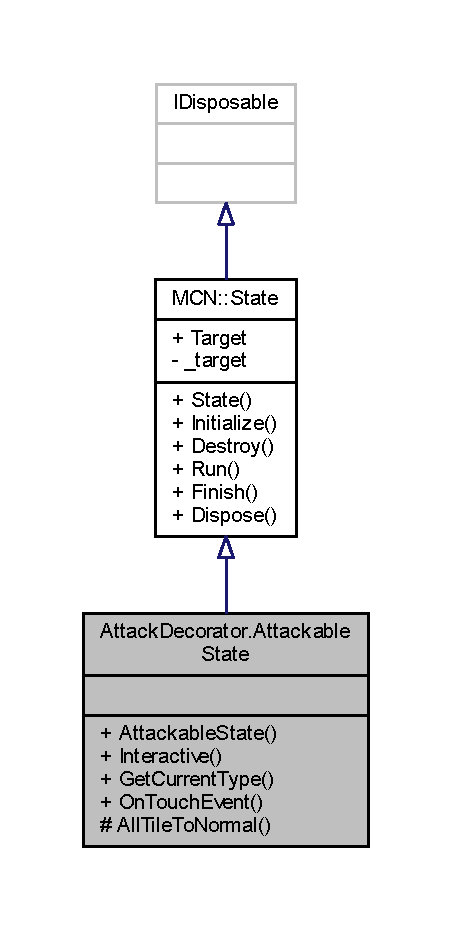
\includegraphics[width=217pt]{class_attack_decorator_1_1_attackable_state__inherit__graph}
\end{center}
\end{figure}


Attack\+Decorator.\+Attackable\+State에 대한 협력 다이어그램\+:
\nopagebreak
\begin{figure}[H]
\begin{center}
\leavevmode
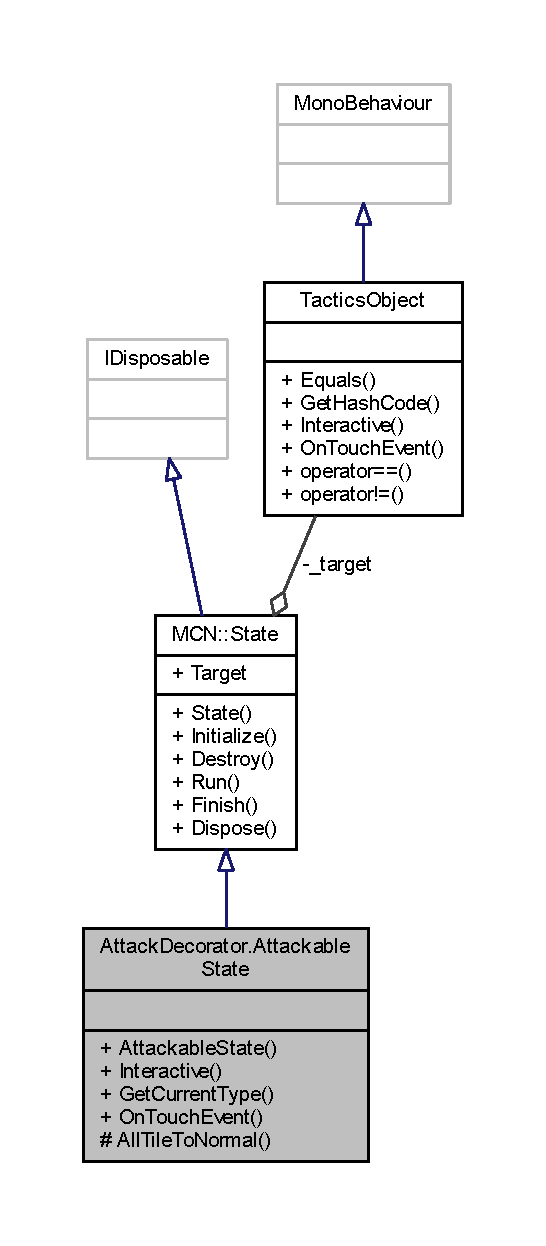
\includegraphics[height=550pt]{class_attack_decorator_1_1_attackable_state__coll__graph}
\end{center}
\end{figure}
\subsection*{Public 멤버 함수}
\begin{DoxyCompactItemize}
\item 
\hyperlink{class_attack_decorator_1_1_attackable_state_ab42449bc9d397049c81f2a6e6d2ac9b7}{Attackable\+State} (\hyperlink{class_tactics_object}{Tactics\+Object} target)
\item 
virtual void \hyperlink{class_attack_decorator_1_1_attackable_state_a8dc1edc91e271393dc3097e92c9563a3}{Interactive} (\hyperlink{class_placeable_object}{Placeable\+Object} target)
\item 
abstract \hyperlink{_attack_decorator_8cs_a11dd66d5fec1bd5b34c8ca6934344cad}{e\+Attackable\+Type} \hyperlink{class_attack_decorator_1_1_attackable_state_a02247dd3afd57a7c3a81540b192fbaa7}{Get\+Current\+Type} ()
\item 
abstract bool \hyperlink{class_attack_decorator_1_1_attackable_state_ac9cf679f51eb8a57cab007476c583dca}{On\+Touch\+Event} ()
\item 
virtual void \hyperlink{class_m_c_n_1_1_state_a5be59bc891e64cbbe4322d74a6746908}{Initialize} ()
\item 
virtual void \hyperlink{class_m_c_n_1_1_state_aebf48ef248bbf185d6aae91d9789459e}{Destroy} ()
\item 
abstract void \hyperlink{class_m_c_n_1_1_state_afdec72a816a8a8ec584cac758a027215}{Run} ()
\item 
virtual void \hyperlink{class_m_c_n_1_1_state_a2492ca731678b8216c02134dddeeb745}{Finish} ()
\item 
void \hyperlink{class_m_c_n_1_1_state_af6df0477e0dead784489688cb2c2093e}{Dispose} ()
\end{DoxyCompactItemize}
\subsection*{Protected 멤버 함수}
\begin{DoxyCompactItemize}
\item 
void \hyperlink{class_attack_decorator_1_1_attackable_state_ad1be8431e8606ed79d375fe520b65e47}{All\+Tile\+To\+Normal} ()
\end{DoxyCompactItemize}
\subsection*{속성}
\begin{DoxyCompactItemize}
\item 
\hyperlink{class_tactics_object}{Tactics\+Object} \hyperlink{class_m_c_n_1_1_state_a79a563b32f183c9adc9a96679fc57eb8}{Target}\hspace{0.3cm}{\ttfamily  \mbox{[}get\mbox{]}}
\end{DoxyCompactItemize}


\subsection{상세한 설명}


Attack\+Decorator.\+cs 파일의 40 번째 라인에서 정의되었습니다.



\subsection{생성자 \& 소멸자 문서화}
\index{Attack\+Decorator\+::\+Attackable\+State@{Attack\+Decorator\+::\+Attackable\+State}!Attackable\+State@{Attackable\+State}}
\index{Attackable\+State@{Attackable\+State}!Attack\+Decorator\+::\+Attackable\+State@{Attack\+Decorator\+::\+Attackable\+State}}
\subsubsection[{\texorpdfstring{Attackable\+State(\+Tactics\+Object target)}{AttackableState(TacticsObject target)}}]{\setlength{\rightskip}{0pt plus 5cm}Attack\+Decorator.\+Attackable\+State.\+Attackable\+State (
\begin{DoxyParamCaption}
\item[{{\bf Tactics\+Object}}]{target}
\end{DoxyParamCaption}
)}\hypertarget{class_attack_decorator_1_1_attackable_state_ab42449bc9d397049c81f2a6e6d2ac9b7}{}\label{class_attack_decorator_1_1_attackable_state_ab42449bc9d397049c81f2a6e6d2ac9b7}


Attack\+Decorator.\+cs 파일의 42 번째 라인에서 정의되었습니다.


\begin{DoxyCode}
42                                                      : base(target)
43         \{
44             var attackable = target as \hyperlink{class_attack_decorator}{AttackDecorator};
45 
46             \textcolor{keywordflow}{if} (attackable != null && attackable.\_attackableStateMachine != null)
47             \{
48                 attackable.\hyperlink{class_attack_decorator_a0ddeffefa8d7bce11d4681c07c50183c}{\_attackableStateMachine}.StorageState(
      \hyperlink{class_attack_decorator_1_1_attackable_state_a02247dd3afd57a7c3a81540b192fbaa7}{GetCurrentType}().ToString(), \textcolor{keyword}{this});
49             \}
50         \}
\end{DoxyCode}


이 함수 내부에서 호출하는 함수들에 대한 그래프입니다.\+:
\nopagebreak
\begin{figure}[H]
\begin{center}
\leavevmode
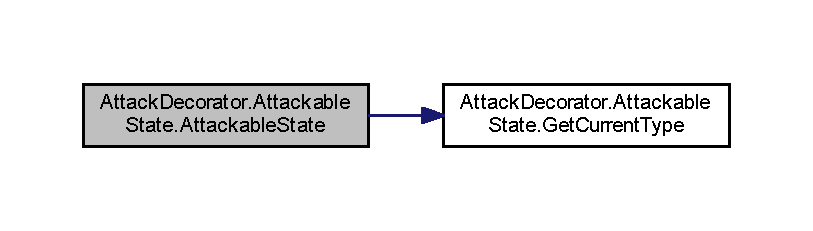
\includegraphics[width=350pt]{class_attack_decorator_1_1_attackable_state_ab42449bc9d397049c81f2a6e6d2ac9b7_cgraph}
\end{center}
\end{figure}




이 함수를 호출하는 함수들에 대한 그래프입니다.\+:
\nopagebreak
\begin{figure}[H]
\begin{center}
\leavevmode
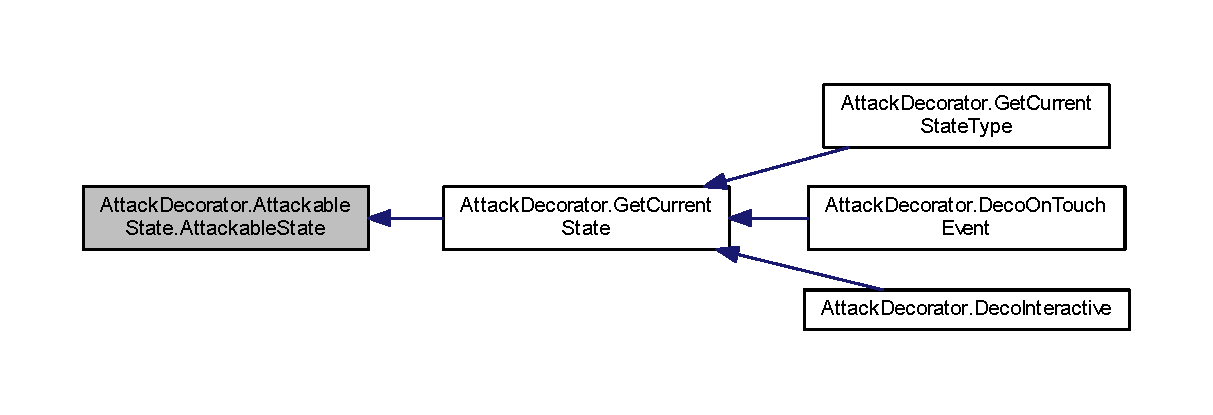
\includegraphics[width=350pt]{class_attack_decorator_1_1_attackable_state_ab42449bc9d397049c81f2a6e6d2ac9b7_icgraph}
\end{center}
\end{figure}




\subsection{멤버 함수 문서화}
\index{Attack\+Decorator\+::\+Attackable\+State@{Attack\+Decorator\+::\+Attackable\+State}!All\+Tile\+To\+Normal@{All\+Tile\+To\+Normal}}
\index{All\+Tile\+To\+Normal@{All\+Tile\+To\+Normal}!Attack\+Decorator\+::\+Attackable\+State@{Attack\+Decorator\+::\+Attackable\+State}}
\subsubsection[{\texorpdfstring{All\+Tile\+To\+Normal()}{AllTileToNormal()}}]{\setlength{\rightskip}{0pt plus 5cm}void Attack\+Decorator.\+Attackable\+State.\+All\+Tile\+To\+Normal (
\begin{DoxyParamCaption}
{}
\end{DoxyParamCaption}
)\hspace{0.3cm}{\ttfamily [protected]}}\hypertarget{class_attack_decorator_1_1_attackable_state_ad1be8431e8606ed79d375fe520b65e47}{}\label{class_attack_decorator_1_1_attackable_state_ad1be8431e8606ed79d375fe520b65e47}


Attack\+Decorator.\+cs 파일의 58 번째 라인에서 정의되었습니다.


\begin{DoxyCode}
59         \{
60             var attackable = \hyperlink{class_m_c_n_1_1_state_a79a563b32f183c9adc9a96679fc57eb8}{Target} as \hyperlink{class_attack_decorator}{AttackDecorator};
61 
62             \textcolor{keywordflow}{if} (attackable != null)
63             \{
64                 var placeable = attackable.\hyperlink{class_m_c_n_1_1_decorator_a1306a0a8b814650cd5970a1ffc7ba2fe}{DecoTarget} as 
      \hyperlink{class_placeable_object}{PlaceableObject};
65 
66                 \textcolor{keywordflow}{if} (placeable != null)
67                 \{
68                     placeable.\hyperlink{class_placeable_object_a0c1248b1f9981ddbf68e6f70a6498f3d}{Deselect}();
69 
70                     \hyperlink{class_map_manager}{MapManager}.\hyperlink{class_m_c_n_1_1_mono_singletone_aa50c027cca64cf4ad30c1ee5c83e0b78}{Instance}.ChangeAllTileState(
      \hyperlink{_tile_8cs_a271bc07be325bca511bcb747e0ff2fda}{eTileType}.NORMAL);
71                 \}
72             \}
73         \}
\end{DoxyCode}


이 함수 내부에서 호출하는 함수들에 대한 그래프입니다.\+:
\nopagebreak
\begin{figure}[H]
\begin{center}
\leavevmode
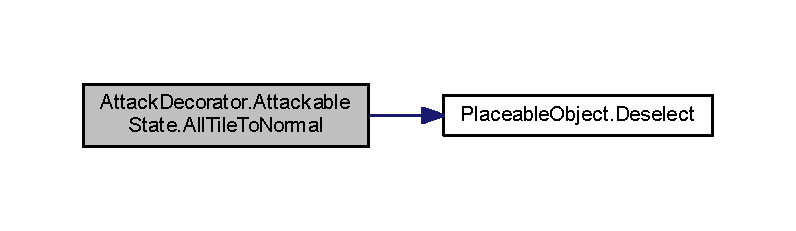
\includegraphics[width=350pt]{class_attack_decorator_1_1_attackable_state_ad1be8431e8606ed79d375fe520b65e47_cgraph}
\end{center}
\end{figure}


\index{Attack\+Decorator\+::\+Attackable\+State@{Attack\+Decorator\+::\+Attackable\+State}!Destroy@{Destroy}}
\index{Destroy@{Destroy}!Attack\+Decorator\+::\+Attackable\+State@{Attack\+Decorator\+::\+Attackable\+State}}
\subsubsection[{\texorpdfstring{Destroy()}{Destroy()}}]{\setlength{\rightskip}{0pt plus 5cm}virtual void M\+C\+N.\+State.\+Destroy (
\begin{DoxyParamCaption}
{}
\end{DoxyParamCaption}
)\hspace{0.3cm}{\ttfamily [virtual]}, {\ttfamily [inherited]}}\hypertarget{class_m_c_n_1_1_state_aebf48ef248bbf185d6aae91d9789459e}{}\label{class_m_c_n_1_1_state_aebf48ef248bbf185d6aae91d9789459e}


State.\+cs 파일의 32 번째 라인에서 정의되었습니다.


\begin{DoxyCode}
32 \{ \}
\end{DoxyCode}


이 함수 내부에서 호출하는 함수들에 대한 그래프입니다.\+:\nopagebreak
\begin{figure}[H]
\begin{center}
\leavevmode
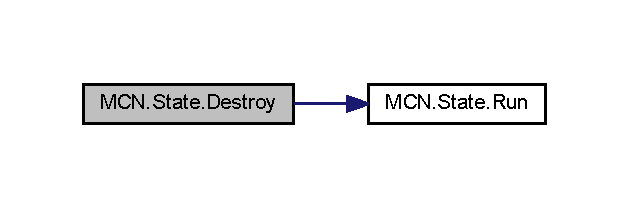
\includegraphics[width=302pt]{class_m_c_n_1_1_state_aebf48ef248bbf185d6aae91d9789459e_cgraph}
\end{center}
\end{figure}




이 함수를 호출하는 함수들에 대한 그래프입니다.\+:\nopagebreak
\begin{figure}[H]
\begin{center}
\leavevmode
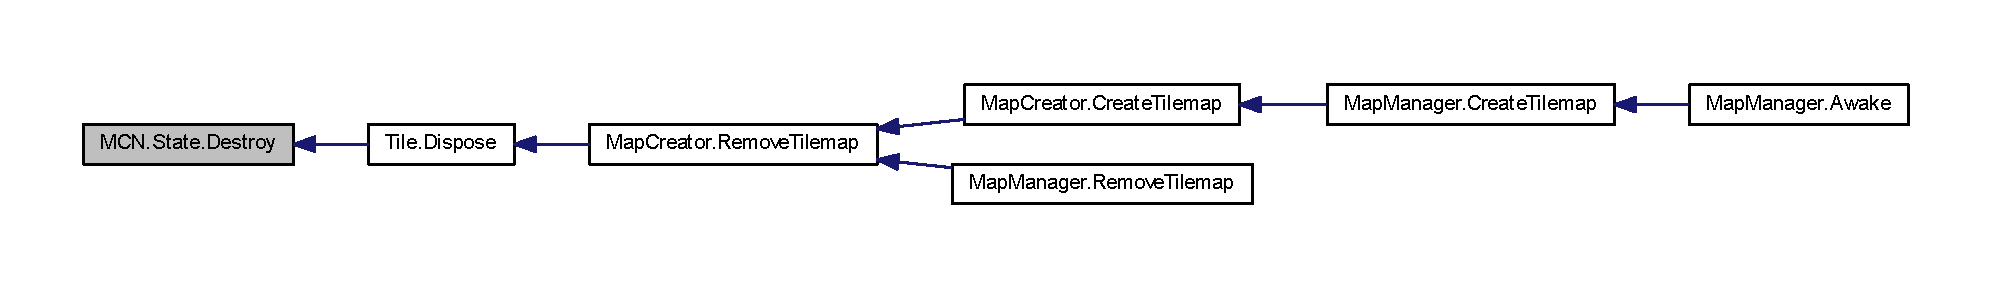
\includegraphics[width=350pt]{class_m_c_n_1_1_state_aebf48ef248bbf185d6aae91d9789459e_icgraph}
\end{center}
\end{figure}


\index{Attack\+Decorator\+::\+Attackable\+State@{Attack\+Decorator\+::\+Attackable\+State}!Dispose@{Dispose}}
\index{Dispose@{Dispose}!Attack\+Decorator\+::\+Attackable\+State@{Attack\+Decorator\+::\+Attackable\+State}}
\subsubsection[{\texorpdfstring{Dispose()}{Dispose()}}]{\setlength{\rightskip}{0pt plus 5cm}void M\+C\+N.\+State.\+Dispose (
\begin{DoxyParamCaption}
{}
\end{DoxyParamCaption}
)\hspace{0.3cm}{\ttfamily [inherited]}}\hypertarget{class_m_c_n_1_1_state_af6df0477e0dead784489688cb2c2093e}{}\label{class_m_c_n_1_1_state_af6df0477e0dead784489688cb2c2093e}


State.\+cs 파일의 37 번째 라인에서 정의되었습니다.


\begin{DoxyCode}
38         \{
39             \hyperlink{class_m_c_n_1_1_state_a13fe398868da354cfde9ff644e12e9f2}{\_target} = null;
40         \}
\end{DoxyCode}


이 함수를 호출하는 함수들에 대한 그래프입니다.\+:\nopagebreak
\begin{figure}[H]
\begin{center}
\leavevmode
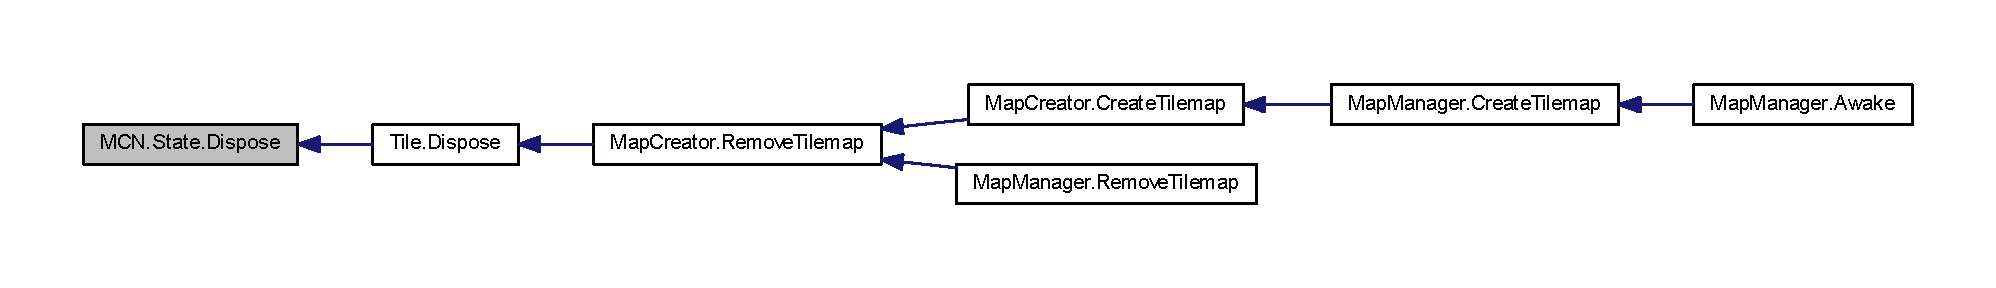
\includegraphics[width=350pt]{class_m_c_n_1_1_state_af6df0477e0dead784489688cb2c2093e_icgraph}
\end{center}
\end{figure}


\index{Attack\+Decorator\+::\+Attackable\+State@{Attack\+Decorator\+::\+Attackable\+State}!Finish@{Finish}}
\index{Finish@{Finish}!Attack\+Decorator\+::\+Attackable\+State@{Attack\+Decorator\+::\+Attackable\+State}}
\subsubsection[{\texorpdfstring{Finish()}{Finish()}}]{\setlength{\rightskip}{0pt plus 5cm}virtual void M\+C\+N.\+State.\+Finish (
\begin{DoxyParamCaption}
{}
\end{DoxyParamCaption}
)\hspace{0.3cm}{\ttfamily [virtual]}, {\ttfamily [inherited]}}\hypertarget{class_m_c_n_1_1_state_a2492ca731678b8216c02134dddeeb745}{}\label{class_m_c_n_1_1_state_a2492ca731678b8216c02134dddeeb745}


State.\+cs 파일의 35 번째 라인에서 정의되었습니다.


\begin{DoxyCode}
35 \{ \}
\end{DoxyCode}
\index{Attack\+Decorator\+::\+Attackable\+State@{Attack\+Decorator\+::\+Attackable\+State}!Get\+Current\+Type@{Get\+Current\+Type}}
\index{Get\+Current\+Type@{Get\+Current\+Type}!Attack\+Decorator\+::\+Attackable\+State@{Attack\+Decorator\+::\+Attackable\+State}}
\subsubsection[{\texorpdfstring{Get\+Current\+Type()}{GetCurrentType()}}]{\setlength{\rightskip}{0pt plus 5cm}abstract {\bf e\+Attackable\+Type} Attack\+Decorator.\+Attackable\+State.\+Get\+Current\+Type (
\begin{DoxyParamCaption}
{}
\end{DoxyParamCaption}
)\hspace{0.3cm}{\ttfamily [pure virtual]}}\hypertarget{class_attack_decorator_1_1_attackable_state_a02247dd3afd57a7c3a81540b192fbaa7}{}\label{class_attack_decorator_1_1_attackable_state_a02247dd3afd57a7c3a81540b192fbaa7}


이 함수를 호출하는 함수들에 대한 그래프입니다.\+:
\nopagebreak
\begin{figure}[H]
\begin{center}
\leavevmode
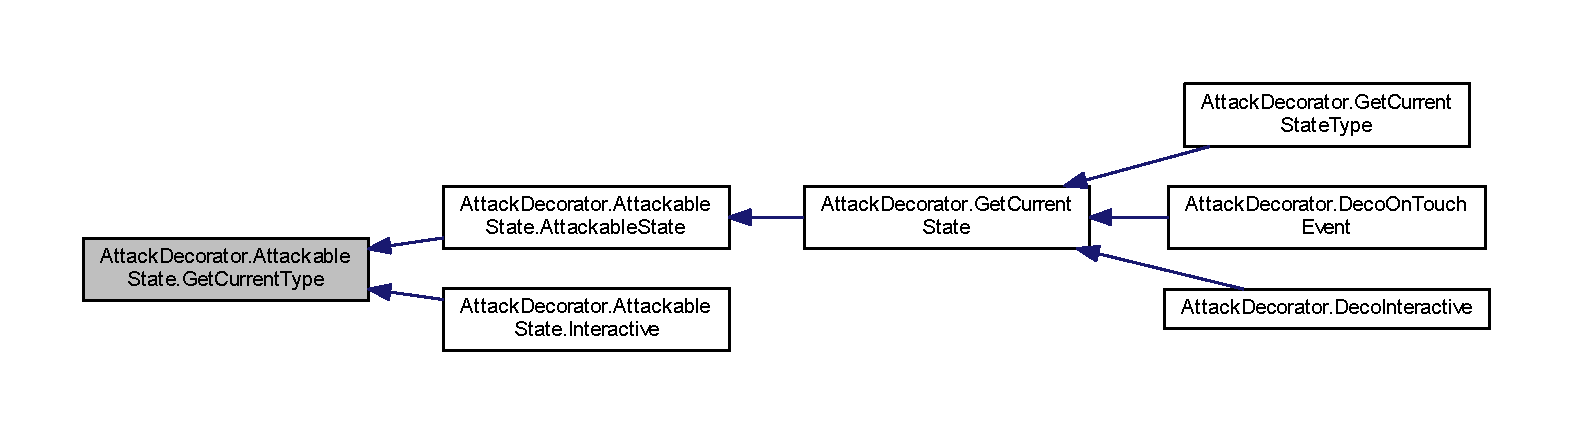
\includegraphics[width=350pt]{class_attack_decorator_1_1_attackable_state_a02247dd3afd57a7c3a81540b192fbaa7_icgraph}
\end{center}
\end{figure}


\index{Attack\+Decorator\+::\+Attackable\+State@{Attack\+Decorator\+::\+Attackable\+State}!Initialize@{Initialize}}
\index{Initialize@{Initialize}!Attack\+Decorator\+::\+Attackable\+State@{Attack\+Decorator\+::\+Attackable\+State}}
\subsubsection[{\texorpdfstring{Initialize()}{Initialize()}}]{\setlength{\rightskip}{0pt plus 5cm}virtual void M\+C\+N.\+State.\+Initialize (
\begin{DoxyParamCaption}
{}
\end{DoxyParamCaption}
)\hspace{0.3cm}{\ttfamily [virtual]}, {\ttfamily [inherited]}}\hypertarget{class_m_c_n_1_1_state_a5be59bc891e64cbbe4322d74a6746908}{}\label{class_m_c_n_1_1_state_a5be59bc891e64cbbe4322d74a6746908}


State.\+cs 파일의 31 번째 라인에서 정의되었습니다.


\begin{DoxyCode}
31 \{ \}
\end{DoxyCode}


이 함수를 호출하는 함수들에 대한 그래프입니다.\+:\nopagebreak
\begin{figure}[H]
\begin{center}
\leavevmode
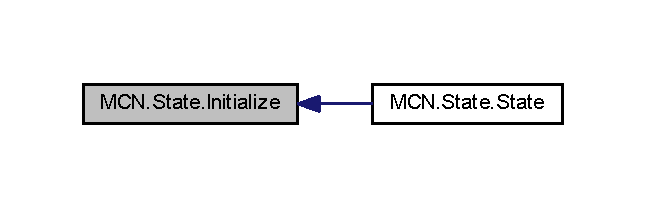
\includegraphics[width=310pt]{class_m_c_n_1_1_state_a5be59bc891e64cbbe4322d74a6746908_icgraph}
\end{center}
\end{figure}


\index{Attack\+Decorator\+::\+Attackable\+State@{Attack\+Decorator\+::\+Attackable\+State}!Interactive@{Interactive}}
\index{Interactive@{Interactive}!Attack\+Decorator\+::\+Attackable\+State@{Attack\+Decorator\+::\+Attackable\+State}}
\subsubsection[{\texorpdfstring{Interactive(\+Placeable\+Object target)}{Interactive(PlaceableObject target)}}]{\setlength{\rightskip}{0pt plus 5cm}virtual void Attack\+Decorator.\+Attackable\+State.\+Interactive (
\begin{DoxyParamCaption}
\item[{{\bf Placeable\+Object}}]{target}
\end{DoxyParamCaption}
)\hspace{0.3cm}{\ttfamily [virtual]}}\hypertarget{class_attack_decorator_1_1_attackable_state_a8dc1edc91e271393dc3097e92c9563a3}{}\label{class_attack_decorator_1_1_attackable_state_a8dc1edc91e271393dc3097e92c9563a3}


Attack\+Decorator.\+cs 파일의 52 번째 라인에서 정의되었습니다.


\begin{DoxyCode}
52 \{ \}
\end{DoxyCode}


이 함수 내부에서 호출하는 함수들에 대한 그래프입니다.\+:
\nopagebreak
\begin{figure}[H]
\begin{center}
\leavevmode
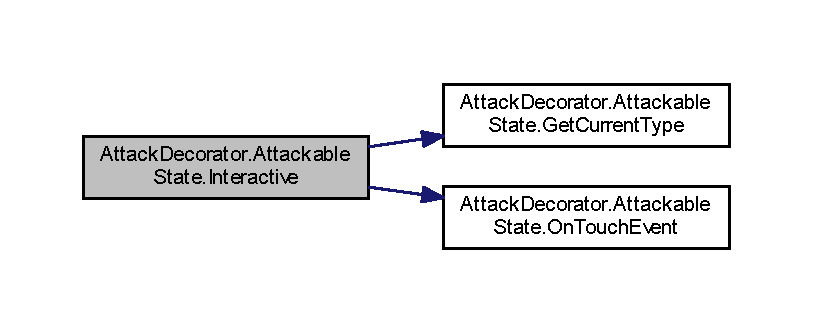
\includegraphics[width=350pt]{class_attack_decorator_1_1_attackable_state_a8dc1edc91e271393dc3097e92c9563a3_cgraph}
\end{center}
\end{figure}


\index{Attack\+Decorator\+::\+Attackable\+State@{Attack\+Decorator\+::\+Attackable\+State}!On\+Touch\+Event@{On\+Touch\+Event}}
\index{On\+Touch\+Event@{On\+Touch\+Event}!Attack\+Decorator\+::\+Attackable\+State@{Attack\+Decorator\+::\+Attackable\+State}}
\subsubsection[{\texorpdfstring{On\+Touch\+Event()}{OnTouchEvent()}}]{\setlength{\rightskip}{0pt plus 5cm}abstract bool Attack\+Decorator.\+Attackable\+State.\+On\+Touch\+Event (
\begin{DoxyParamCaption}
{}
\end{DoxyParamCaption}
)\hspace{0.3cm}{\ttfamily [pure virtual]}}\hypertarget{class_attack_decorator_1_1_attackable_state_ac9cf679f51eb8a57cab007476c583dca}{}\label{class_attack_decorator_1_1_attackable_state_ac9cf679f51eb8a57cab007476c583dca}


이 함수를 호출하는 함수들에 대한 그래프입니다.\+:
\nopagebreak
\begin{figure}[H]
\begin{center}
\leavevmode
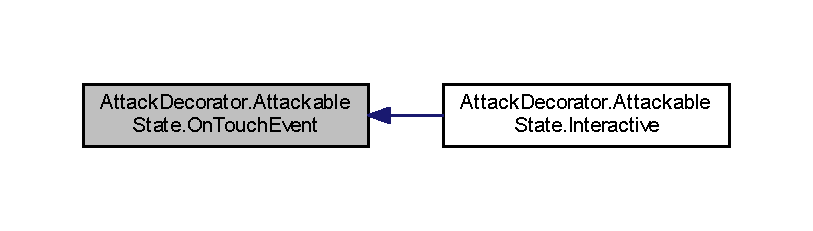
\includegraphics[width=350pt]{class_attack_decorator_1_1_attackable_state_ac9cf679f51eb8a57cab007476c583dca_icgraph}
\end{center}
\end{figure}


\index{Attack\+Decorator\+::\+Attackable\+State@{Attack\+Decorator\+::\+Attackable\+State}!Run@{Run}}
\index{Run@{Run}!Attack\+Decorator\+::\+Attackable\+State@{Attack\+Decorator\+::\+Attackable\+State}}
\subsubsection[{\texorpdfstring{Run()}{Run()}}]{\setlength{\rightskip}{0pt plus 5cm}abstract void M\+C\+N.\+State.\+Run (
\begin{DoxyParamCaption}
{}
\end{DoxyParamCaption}
)\hspace{0.3cm}{\ttfamily [pure virtual]}, {\ttfamily [inherited]}}\hypertarget{class_m_c_n_1_1_state_afdec72a816a8a8ec584cac758a027215}{}\label{class_m_c_n_1_1_state_afdec72a816a8a8ec584cac758a027215}


\hyperlink{class_move_decorator_1_1_moveable_state___done_ad6aac25a9f42d14a958d1c93e3b6bd79}{Move\+Decorator.\+Moveable\+State\+\_\+\+Done}, \hyperlink{class_move_decorator_1_1_moveable_state___normal_a9e4e591aa61c13840a15facffa2148d6}{Move\+Decorator.\+Moveable\+State\+\_\+\+Normal}, \hyperlink{class_tile_1_1_tile_state___deactive_a806c5dbc5eb43903ad41d448f3d25c61}{Tile.\+Tile\+State\+\_\+\+Deactive}, \hyperlink{class_move_decorator_1_1_moveable_state___move_ae1bb2c9ca5992373aa872788775d3e4a}{Move\+Decorator.\+Moveable\+State\+\_\+\+Move}, \hyperlink{class_tile_1_1_tile_state___active_ab53c7c818d65122d6d36c9681ca53bf9}{Tile.\+Tile\+State\+\_\+\+Active}, \hyperlink{class_tile_1_1_tile_state___normal_acf613382b6ddeff2fcc226d8caeb0b53}{Tile.\+Tile\+State\+\_\+\+Normal}에서 구현되었습니다.



이 함수를 호출하는 함수들에 대한 그래프입니다.\+:\nopagebreak
\begin{figure}[H]
\begin{center}
\leavevmode
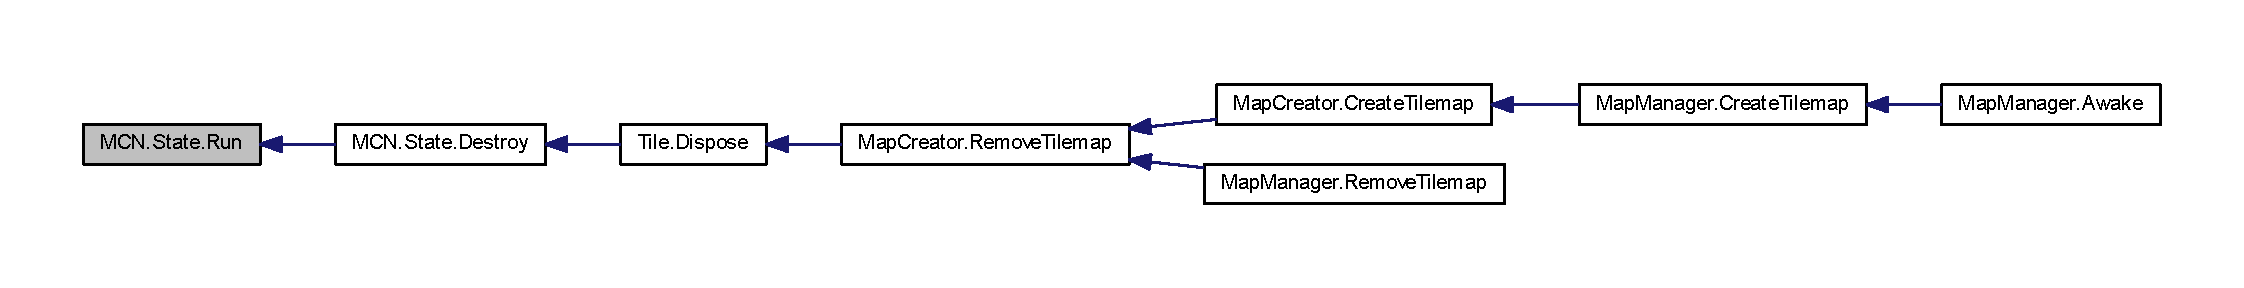
\includegraphics[width=350pt]{class_m_c_n_1_1_state_afdec72a816a8a8ec584cac758a027215_icgraph}
\end{center}
\end{figure}




\subsection{속성 문서화}
\index{Attack\+Decorator\+::\+Attackable\+State@{Attack\+Decorator\+::\+Attackable\+State}!Target@{Target}}
\index{Target@{Target}!Attack\+Decorator\+::\+Attackable\+State@{Attack\+Decorator\+::\+Attackable\+State}}
\subsubsection[{\texorpdfstring{Target}{Target}}]{\setlength{\rightskip}{0pt plus 5cm}{\bf Tactics\+Object} M\+C\+N.\+State.\+Target\hspace{0.3cm}{\ttfamily [get]}, {\ttfamily [protected]}, {\ttfamily [inherited]}}\hypertarget{class_m_c_n_1_1_state_a79a563b32f183c9adc9a96679fc57eb8}{}\label{class_m_c_n_1_1_state_a79a563b32f183c9adc9a96679fc57eb8}


State.\+cs 파일의 17 번째 라인에서 정의되었습니다.



이 클래스에 대한 문서화 페이지는 다음의 파일로부터 생성되었습니다.\+:\begin{DoxyCompactItemize}
\item 
D\+:/\+Git\+Hub/\+M\+C\+N\+Tactics/\+Assets/\+Scripts/\+Objects/\+Decorator/\hyperlink{_attack_decorator_8cs}{Attack\+Decorator.\+cs}\end{DoxyCompactItemize}

\hypertarget{class_attack_decorator}{}\section{Attack\+Decorator 클래스 참조}
\label{class_attack_decorator}\index{Attack\+Decorator@{Attack\+Decorator}}


Attack\+Decorator에 대한 상속 다이어그램 \+: 
\nopagebreak
\begin{figure}[H]
\begin{center}
\leavevmode
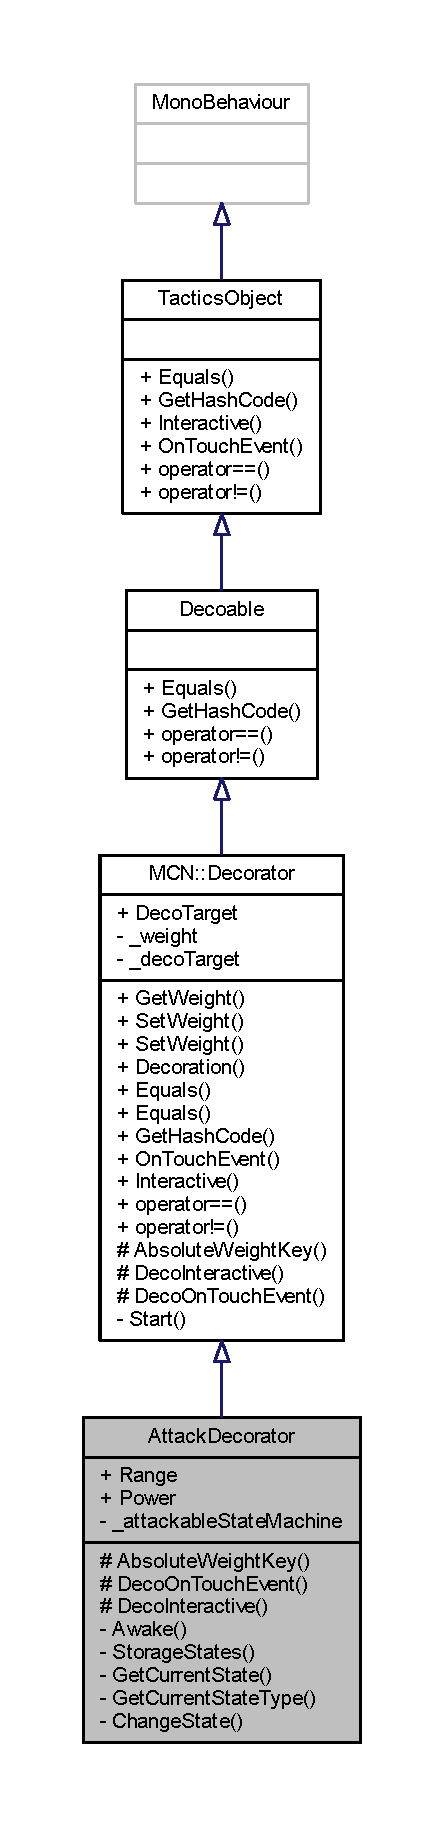
\includegraphics[height=550pt]{class_attack_decorator__inherit__graph}
\end{center}
\end{figure}


Attack\+Decorator에 대한 협력 다이어그램\+:
\nopagebreak
\begin{figure}[H]
\begin{center}
\leavevmode
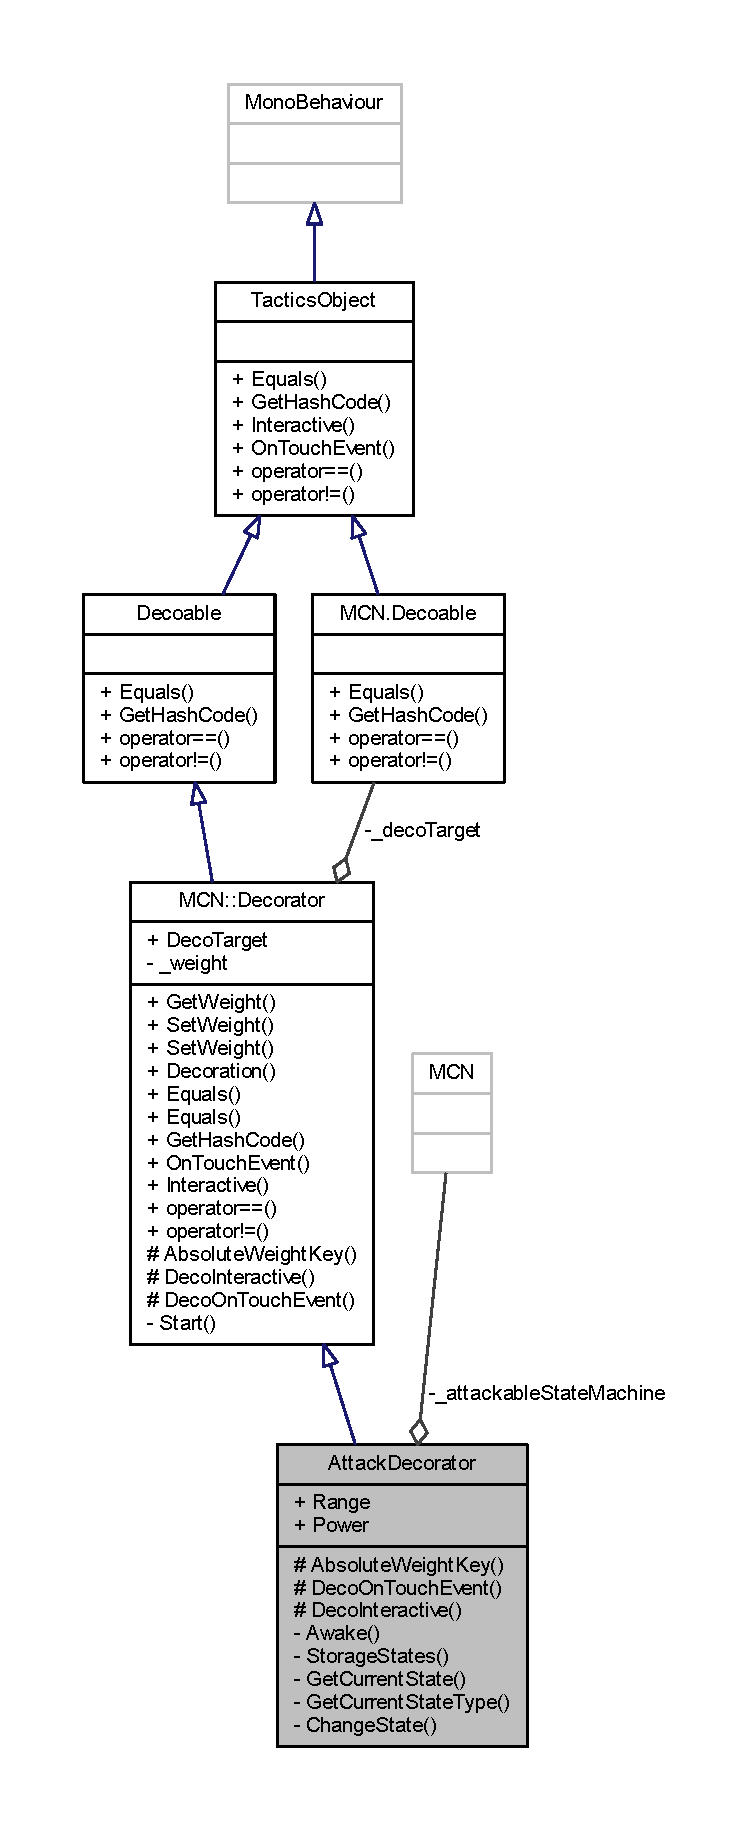
\includegraphics[height=550pt]{class_attack_decorator__coll__graph}
\end{center}
\end{figure}
\subsection*{클래스}
\begin{DoxyCompactItemize}
\item 
class \hyperlink{class_attack_decorator_1_1_attackable_state}{Attackable\+State}
\end{DoxyCompactItemize}
\subsection*{Public 멤버 함수}
\begin{DoxyCompactItemize}
\item 
int \hyperlink{class_m_c_n_1_1_decorator_a2fa8df5e51cc3fdaa63b28c4e4917670}{Get\+Weight} (string key)
\item 
void \hyperlink{class_m_c_n_1_1_decorator_a0658f2776c28dad0517b56085910162c}{Set\+Weight} (string key, int weight)
\item 
void \hyperlink{class_m_c_n_1_1_decorator_aa64c6b8a8f30f4e8083da6dd0fab226c}{Set\+Weight} (Pair$<$ string, int $>$ info)
\item 
void \hyperlink{class_m_c_n_1_1_decorator_ab82c83f62182a25a72dc81530c743c32}{Decoration} (Decoable target)
\item 
override bool \hyperlink{class_m_c_n_1_1_decorator_ae2a5432ce00298c80dcb433a75bbe45d}{Equals} (object o)
\item 
bool \hyperlink{class_m_c_n_1_1_decorator_a3ad7a8cf76c976907116f85a65a9f8e9}{Equals} (Deco\+Instance o)
\item 
override int \hyperlink{class_m_c_n_1_1_decorator_a6df84cd2af5b096128e84791455c083f}{Get\+Hash\+Code} ()
\item 
sealed override bool \hyperlink{class_m_c_n_1_1_decorator_ac45ab12c190bd9f5188c9f748f8ddbbf}{On\+Touch\+Event} (\hyperlink{_touch_manager_8cs_ae33e321a424fe84ba8b2fdb81ad40a68}{e\+Touch\+Event} touch)
\item 
sealed override void \hyperlink{class_m_c_n_1_1_decorator_ae58cb79cf1ee47006b7dbdac82b97dc5}{Interactive} (\hyperlink{class_tactics_object}{Tactics\+Object} interact\+Target)
\end{DoxyCompactItemize}
\subsection*{정적 Public 멤버 함수}
\begin{DoxyCompactItemize}
\item 
static bool \hyperlink{class_m_c_n_1_1_decorator_a4c4c97e4a4dcf1a66e764740a5bbf3c6}{operator==} (Decorator lt, Deco\+Instance rt)
\item 
static bool \hyperlink{class_m_c_n_1_1_decoable_a6004bbc5f208c3031388c9d6e8f8359b}{operator==} (Decoable lt, Decoable rt)
\item 
static bool \hyperlink{class_tactics_object_a18f2979a4bf81dc755fbc17e425809f0}{operator==} (\hyperlink{class_tactics_object}{Tactics\+Object} lt, \hyperlink{class_tactics_object}{Tactics\+Object} rt)
\item 
static bool \hyperlink{class_m_c_n_1_1_decorator_a89e2f61a0974c51610a0c8d14ef6962a}{operator!=} (Decorator lt, Deco\+Instance rt)
\item 
static bool \hyperlink{class_m_c_n_1_1_decoable_aa75e4102ebd7265f577028b407534d27}{operator!=} (Decoable lt, Decoable rt)
\item 
static bool \hyperlink{class_tactics_object_a49e235618a22126faa6271243cd89710}{operator!=} (\hyperlink{class_tactics_object}{Tactics\+Object} lt, \hyperlink{class_tactics_object}{Tactics\+Object} rt)
\end{DoxyCompactItemize}
\subsection*{Protected 멤버 함수}
\begin{DoxyCompactItemize}
\item 
override string\mbox{[}$\,$\mbox{]} \hyperlink{class_attack_decorator_aa0fdb6701a08f63d011aacf6bd6d6df7}{Absolute\+Weight\+Key} ()
\item 
override bool \hyperlink{class_attack_decorator_abff1ff6a1fa1b896f3f0251cf7652eb0}{Deco\+On\+Touch\+Event} (\hyperlink{_touch_manager_8cs_ae33e321a424fe84ba8b2fdb81ad40a68}{e\+Touch\+Event} touch)
\item 
override void \hyperlink{class_attack_decorator_ac0de076a7e28dbb6253aa5b1555195b3}{Deco\+Interactive} (\hyperlink{class_tactics_object}{Tactics\+Object} interact\+Target)
\end{DoxyCompactItemize}
\subsection*{속성}
\begin{DoxyCompactItemize}
\item 
int \hyperlink{class_attack_decorator_ad025c4d20cc5dba4326ecbd52562a3c4}{Range}\hspace{0.3cm}{\ttfamily  \mbox{[}get\mbox{]}}
\item 
int \hyperlink{class_attack_decorator_a3305d359c9c0faaf4f12aa261492ee7c}{Power}\hspace{0.3cm}{\ttfamily  \mbox{[}get\mbox{]}}
\item 
\hyperlink{class_m_c_n_1_1_decoable}{M\+C\+N.\+Decoable} \hyperlink{class_m_c_n_1_1_decorator_a1306a0a8b814650cd5970a1ffc7ba2fe}{Deco\+Target}\hspace{0.3cm}{\ttfamily  \mbox{[}get\mbox{]}}
\end{DoxyCompactItemize}
\subsection*{Private 멤버 함수}
\begin{DoxyCompactItemize}
\item 
void \hyperlink{class_attack_decorator_a84bd4b501002dde5aaf3bedad223acad}{Awake} ()
\item 
void \hyperlink{class_attack_decorator_a4c5bb156eda734c19594c740c6d63aad}{Storage\+States} ()
\item 
\hyperlink{class_attack_decorator_1_1_attackable_state}{Attackable\+State} \hyperlink{class_attack_decorator_af56bf418b8ba41fa9c7d8a697e39ce26}{Get\+Current\+State} ()
\item 
\hyperlink{_attack_decorator_8cs_a11dd66d5fec1bd5b34c8ca6934344cad}{e\+Attackable\+Type} \hyperlink{class_attack_decorator_a0fe90a081a8bf36c973b6a9b571c4966}{Get\+Current\+State\+Type} ()
\item 
void \hyperlink{class_attack_decorator_a754ed58a005e35f352b5eef1a9de46b2}{Change\+State} (\hyperlink{_attack_decorator_8cs_a11dd66d5fec1bd5b34c8ca6934344cad}{e\+Attackable\+Type} type)
\end{DoxyCompactItemize}
\subsection*{Private 속성}
\begin{DoxyCompactItemize}
\item 
\hyperlink{class_m_c_n_1_1_state_machine}{M\+C\+N.\+State\+Machine}$<$ \hyperlink{class_attack_decorator_1_1_attackable_state}{Attackable\+State} $>$ \hyperlink{class_attack_decorator_a0ddeffefa8d7bce11d4681c07c50183c}{\+\_\+attackable\+State\+Machine} = new \hyperlink{class_m_c_n_1_1_state_machine}{M\+C\+N.\+State\+Machine}$<$\hyperlink{class_attack_decorator_1_1_attackable_state}{Attackable\+State}$>$()
\end{DoxyCompactItemize}


\subsection{상세한 설명}


Attack\+Decorator.\+cs 파일의 12 번째 라인에서 정의되었습니다.



\subsection{멤버 함수 문서화}
\index{Attack\+Decorator@{Attack\+Decorator}!Absolute\+Weight\+Key@{Absolute\+Weight\+Key}}
\index{Absolute\+Weight\+Key@{Absolute\+Weight\+Key}!Attack\+Decorator@{Attack\+Decorator}}
\subsubsection[{\texorpdfstring{Absolute\+Weight\+Key()}{AbsoluteWeightKey()}}]{\setlength{\rightskip}{0pt plus 5cm}override string \mbox{[}$\,$\mbox{]} Attack\+Decorator.\+Absolute\+Weight\+Key (
\begin{DoxyParamCaption}
{}
\end{DoxyParamCaption}
)\hspace{0.3cm}{\ttfamily [protected]}, {\ttfamily [virtual]}}\hypertarget{class_attack_decorator_aa0fdb6701a08f63d011aacf6bd6d6df7}{}\label{class_attack_decorator_aa0fdb6701a08f63d011aacf6bd6d6df7}


\hyperlink{class_m_c_n_1_1_decorator_add763642ece4015f68d63504291fc783}{M\+C\+N.\+Decorator}를 구현.



Attack\+Decorator.\+cs 파일의 31 번째 라인에서 정의되었습니다.


\begin{DoxyCode}
32     \{
33         \textcolor{keywordflow}{return} \textcolor{keyword}{new} \textcolor{keywordtype}{string}[] \{ \textcolor{stringliteral}{"range"}, \textcolor{stringliteral}{"power"} \};
34     \}
\end{DoxyCode}
\index{Attack\+Decorator@{Attack\+Decorator}!Awake@{Awake}}
\index{Awake@{Awake}!Attack\+Decorator@{Attack\+Decorator}}
\subsubsection[{\texorpdfstring{Awake()}{Awake()}}]{\setlength{\rightskip}{0pt plus 5cm}void Attack\+Decorator.\+Awake (
\begin{DoxyParamCaption}
{}
\end{DoxyParamCaption}
)\hspace{0.3cm}{\ttfamily [private]}}\hypertarget{class_attack_decorator_a84bd4b501002dde5aaf3bedad223acad}{}\label{class_attack_decorator_a84bd4b501002dde5aaf3bedad223acad}


Attack\+Decorator.\+cs 파일의 79 번째 라인에서 정의되었습니다.


\begin{DoxyCode}
80     \{
81         \hyperlink{class_attack_decorator_a4c5bb156eda734c19594c740c6d63aad}{StorageStates}();
82     \}
\end{DoxyCode}


이 함수 내부에서 호출하는 함수들에 대한 그래프입니다.\+:
\nopagebreak
\begin{figure}[H]
\begin{center}
\leavevmode
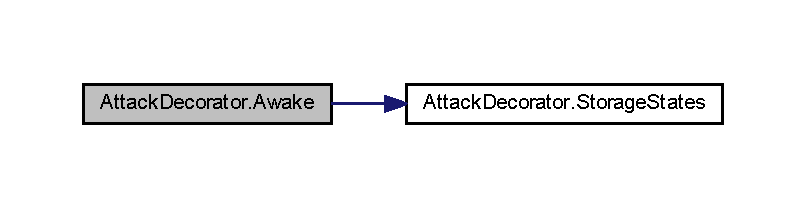
\includegraphics[width=350pt]{class_attack_decorator_a84bd4b501002dde5aaf3bedad223acad_cgraph}
\end{center}
\end{figure}


\index{Attack\+Decorator@{Attack\+Decorator}!Change\+State@{Change\+State}}
\index{Change\+State@{Change\+State}!Attack\+Decorator@{Attack\+Decorator}}
\subsubsection[{\texorpdfstring{Change\+State(e\+Attackable\+Type type)}{ChangeState(eAttackableType type)}}]{\setlength{\rightskip}{0pt plus 5cm}void Attack\+Decorator.\+Change\+State (
\begin{DoxyParamCaption}
\item[{{\bf e\+Attackable\+Type}}]{type}
\end{DoxyParamCaption}
)\hspace{0.3cm}{\ttfamily [private]}}\hypertarget{class_attack_decorator_a754ed58a005e35f352b5eef1a9de46b2}{}\label{class_attack_decorator_a754ed58a005e35f352b5eef1a9de46b2}


Attack\+Decorator.\+cs 파일의 112 번째 라인에서 정의되었습니다.


\begin{DoxyCode}
113     \{
114         \textcolor{keywordflow}{if} (\hyperlink{class_attack_decorator_a0ddeffefa8d7bce11d4681c07c50183c}{\_attackableStateMachine} != null)
115         \{
116             \hyperlink{class_attack_decorator_a0ddeffefa8d7bce11d4681c07c50183c}{\_attackableStateMachine}.ChangeState(type.ToString());
117         \}
118     \}
\end{DoxyCode}
\index{Attack\+Decorator@{Attack\+Decorator}!Deco\+Interactive@{Deco\+Interactive}}
\index{Deco\+Interactive@{Deco\+Interactive}!Attack\+Decorator@{Attack\+Decorator}}
\subsubsection[{\texorpdfstring{Deco\+Interactive(\+Tactics\+Object interact\+Target)}{DecoInteractive(TacticsObject interactTarget)}}]{\setlength{\rightskip}{0pt plus 5cm}override void Attack\+Decorator.\+Deco\+Interactive (
\begin{DoxyParamCaption}
\item[{{\bf Tactics\+Object}}]{interact\+Target}
\end{DoxyParamCaption}
)\hspace{0.3cm}{\ttfamily [protected]}, {\ttfamily [virtual]}}\hypertarget{class_attack_decorator_ac0de076a7e28dbb6253aa5b1555195b3}{}\label{class_attack_decorator_ac0de076a7e28dbb6253aa5b1555195b3}


\hyperlink{class_m_c_n_1_1_decorator_a317f646a9053334fdbe28b9f1ae690a5}{M\+C\+N.\+Decorator}(으)로부터 재구현되었습니다.



Attack\+Decorator.\+cs 파일의 132 번째 라인에서 정의되었습니다.


\begin{DoxyCode}
133     \{
134         var target = interactTarget as \hyperlink{class_placeable_object}{PlaceableObject};
135 
136         \textcolor{keywordflow}{if} (target != null)
137         \{
138             var state = \hyperlink{class_attack_decorator_af56bf418b8ba41fa9c7d8a697e39ce26}{GetCurrentState}();
139 
140             \textcolor{keywordflow}{if} (state != null)
141             \{
142                 state.Interactive(target);
143             \}
144         \}
145     \}
\end{DoxyCode}


이 함수 내부에서 호출하는 함수들에 대한 그래프입니다.\+:
\nopagebreak
\begin{figure}[H]
\begin{center}
\leavevmode
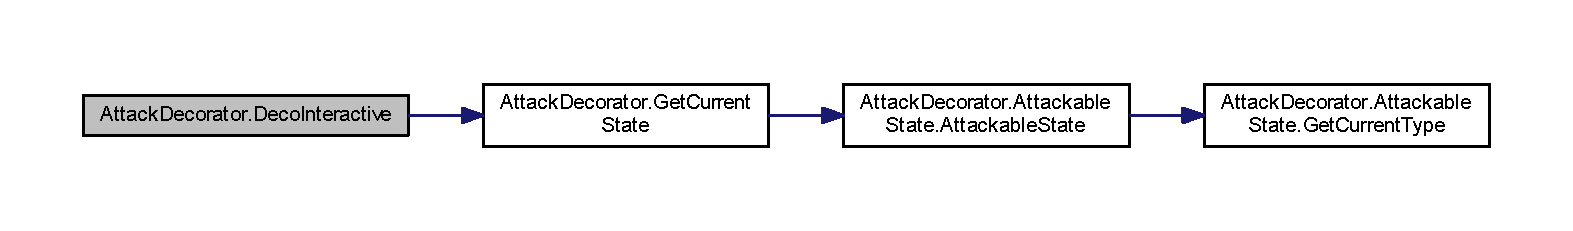
\includegraphics[width=350pt]{class_attack_decorator_ac0de076a7e28dbb6253aa5b1555195b3_cgraph}
\end{center}
\end{figure}


\index{Attack\+Decorator@{Attack\+Decorator}!Deco\+On\+Touch\+Event@{Deco\+On\+Touch\+Event}}
\index{Deco\+On\+Touch\+Event@{Deco\+On\+Touch\+Event}!Attack\+Decorator@{Attack\+Decorator}}
\subsubsection[{\texorpdfstring{Deco\+On\+Touch\+Event(e\+Touch\+Event touch)}{DecoOnTouchEvent(eTouchEvent touch)}}]{\setlength{\rightskip}{0pt plus 5cm}override bool Attack\+Decorator.\+Deco\+On\+Touch\+Event (
\begin{DoxyParamCaption}
\item[{{\bf e\+Touch\+Event}}]{touch}
\end{DoxyParamCaption}
)\hspace{0.3cm}{\ttfamily [protected]}, {\ttfamily [virtual]}}\hypertarget{class_attack_decorator_abff1ff6a1fa1b896f3f0251cf7652eb0}{}\label{class_attack_decorator_abff1ff6a1fa1b896f3f0251cf7652eb0}


\hyperlink{class_m_c_n_1_1_decorator_abc499f6479fad929fc812e218d39a06d}{M\+C\+N.\+Decorator}(으)로부터 재구현되었습니다.



Attack\+Decorator.\+cs 파일의 120 번째 라인에서 정의되었습니다.


\begin{DoxyCode}
121     \{
122         var state = \hyperlink{class_attack_decorator_af56bf418b8ba41fa9c7d8a697e39ce26}{GetCurrentState}();
123 
124         \textcolor{keywordflow}{if} (state != null)
125         \{
126             \textcolor{keywordflow}{return} state.OnTouchEvent();
127         \}
128 
129         \textcolor{keywordflow}{throw} \textcolor{keyword}{new} UnityException(\textcolor{stringliteral}{"don't have attackable state."});
130     \}
\end{DoxyCode}


이 함수 내부에서 호출하는 함수들에 대한 그래프입니다.\+:
\nopagebreak
\begin{figure}[H]
\begin{center}
\leavevmode
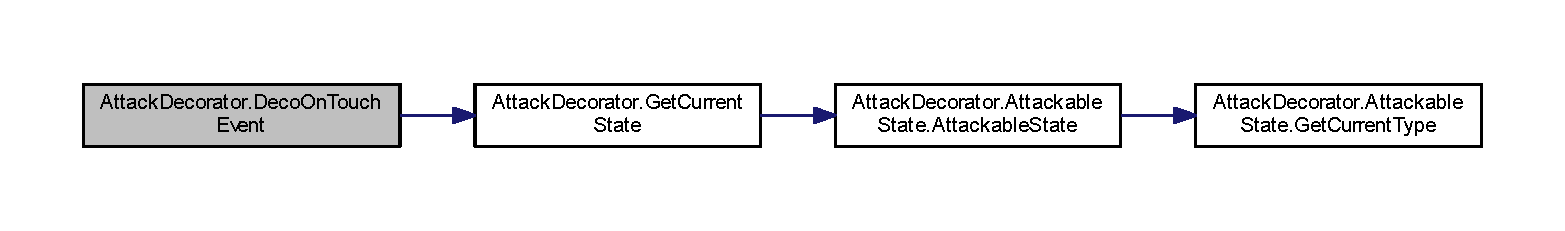
\includegraphics[width=350pt]{class_attack_decorator_abff1ff6a1fa1b896f3f0251cf7652eb0_cgraph}
\end{center}
\end{figure}


\index{Attack\+Decorator@{Attack\+Decorator}!Decoration@{Decoration}}
\index{Decoration@{Decoration}!Attack\+Decorator@{Attack\+Decorator}}
\subsubsection[{\texorpdfstring{Decoration(\+Decoable target)}{Decoration(Decoable target)}}]{\setlength{\rightskip}{0pt plus 5cm}void M\+C\+N.\+Decorator.\+Decoration (
\begin{DoxyParamCaption}
\item[{{\bf Decoable}}]{target}
\end{DoxyParamCaption}
)\hspace{0.3cm}{\ttfamily [inherited]}}\hypertarget{class_m_c_n_1_1_decorator_ab82c83f62182a25a72dc81530c743c32}{}\label{class_m_c_n_1_1_decorator_ab82c83f62182a25a72dc81530c743c32}


Decorator.\+cs 파일의 196 번째 라인에서 정의되었습니다.


\begin{DoxyCode}
197         \{
198             this.\hyperlink{class_m_c_n_1_1_decorator_a1ec6050ce16016f709aa8e8c19444678}{\_decoTarget} = target;
199 
200             var root = \hyperlink{class_m_c_n_1_1_decorator_a1306a0a8b814650cd5970a1ffc7ba2fe}{DecoTarget} as DecoInstance;
201 
202             \textcolor{keywordflow}{if}(root != null)
203             \{
204                 root.Decorated(\textcolor{keyword}{this});
205             \}
206         \}
\end{DoxyCode}


이 함수 내부에서 호출하는 함수들에 대한 그래프입니다.\+:\nopagebreak
\begin{figure}[H]
\begin{center}
\leavevmode
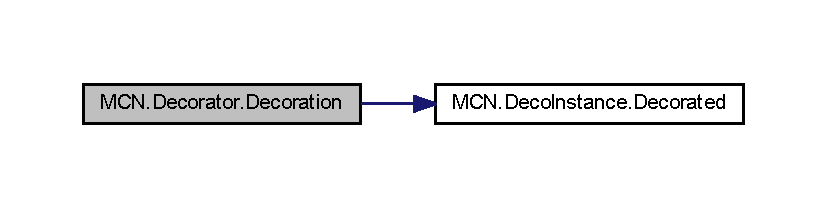
\includegraphics[width=350pt]{class_m_c_n_1_1_decorator_ab82c83f62182a25a72dc81530c743c32_cgraph}
\end{center}
\end{figure}




이 함수를 호출하는 함수들에 대한 그래프입니다.\+:\nopagebreak
\begin{figure}[H]
\begin{center}
\leavevmode
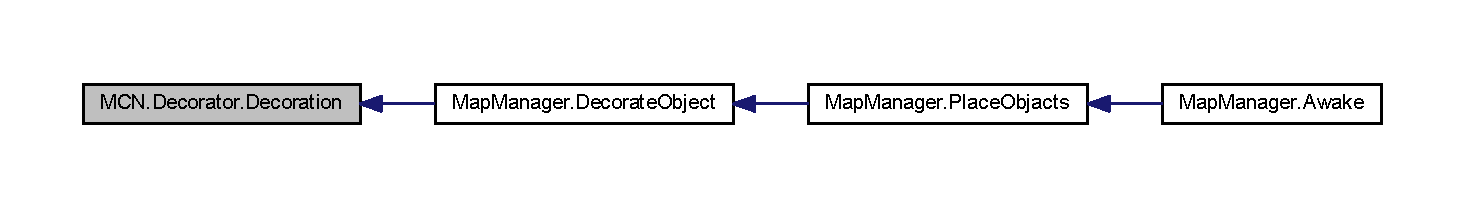
\includegraphics[width=350pt]{class_m_c_n_1_1_decorator_ab82c83f62182a25a72dc81530c743c32_icgraph}
\end{center}
\end{figure}


\index{Attack\+Decorator@{Attack\+Decorator}!Equals@{Equals}}
\index{Equals@{Equals}!Attack\+Decorator@{Attack\+Decorator}}
\subsubsection[{\texorpdfstring{Equals(object o)}{Equals(object o)}}]{\setlength{\rightskip}{0pt plus 5cm}override bool M\+C\+N.\+Decorator.\+Equals (
\begin{DoxyParamCaption}
\item[{object}]{o}
\end{DoxyParamCaption}
)\hspace{0.3cm}{\ttfamily [inherited]}}\hypertarget{class_m_c_n_1_1_decorator_ae2a5432ce00298c80dcb433a75bbe45d}{}\label{class_m_c_n_1_1_decorator_ae2a5432ce00298c80dcb433a75bbe45d}


Decorator.\+cs 파일의 229 번째 라인에서 정의되었습니다.


\begin{DoxyCode}
230         \{
231             \textcolor{keywordflow}{if} (o is DecoInstance)
232             \{
233                 this.\hyperlink{class_m_c_n_1_1_decorator_ae2a5432ce00298c80dcb433a75bbe45d}{Equals}(o as DecoInstance);
234             \}
235 
236             \textcolor{keywordflow}{return} base.Equals(o);
237         \}
\end{DoxyCode}


이 함수 내부에서 호출하는 함수들에 대한 그래프입니다.\+:\nopagebreak
\begin{figure}[H]
\begin{center}
\leavevmode
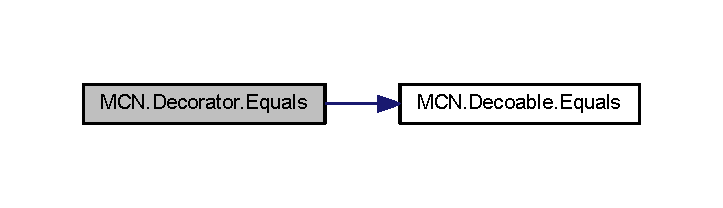
\includegraphics[width=347pt]{class_m_c_n_1_1_decorator_ae2a5432ce00298c80dcb433a75bbe45d_cgraph}
\end{center}
\end{figure}


\index{Attack\+Decorator@{Attack\+Decorator}!Equals@{Equals}}
\index{Equals@{Equals}!Attack\+Decorator@{Attack\+Decorator}}
\subsubsection[{\texorpdfstring{Equals(\+Deco\+Instance o)}{Equals(DecoInstance o)}}]{\setlength{\rightskip}{0pt plus 5cm}bool M\+C\+N.\+Decorator.\+Equals (
\begin{DoxyParamCaption}
\item[{{\bf Deco\+Instance}}]{o}
\end{DoxyParamCaption}
)\hspace{0.3cm}{\ttfamily [inherited]}}\hypertarget{class_m_c_n_1_1_decorator_a3ad7a8cf76c976907116f85a65a9f8e9}{}\label{class_m_c_n_1_1_decorator_a3ad7a8cf76c976907116f85a65a9f8e9}


Decorator.\+cs 파일의 239 번째 라인에서 정의되었습니다.


\begin{DoxyCode}
240         \{
241             \textcolor{keywordflow}{if} (o == null)
242             \{
243                 \textcolor{keywordflow}{return} \textcolor{keyword}{false};
244             \}
245 
246             \textcolor{keywordflow}{return} \textcolor{keyword}{this} == o;
247         \}
\end{DoxyCode}
\index{Attack\+Decorator@{Attack\+Decorator}!Get\+Current\+State@{Get\+Current\+State}}
\index{Get\+Current\+State@{Get\+Current\+State}!Attack\+Decorator@{Attack\+Decorator}}
\subsubsection[{\texorpdfstring{Get\+Current\+State()}{GetCurrentState()}}]{\setlength{\rightskip}{0pt plus 5cm}{\bf Attackable\+State} Attack\+Decorator.\+Get\+Current\+State (
\begin{DoxyParamCaption}
{}
\end{DoxyParamCaption}
)\hspace{0.3cm}{\ttfamily [private]}}\hypertarget{class_attack_decorator_af56bf418b8ba41fa9c7d8a697e39ce26}{}\label{class_attack_decorator_af56bf418b8ba41fa9c7d8a697e39ce26}


Attack\+Decorator.\+cs 파일의 89 번째 라인에서 정의되었습니다.


\begin{DoxyCode}
90     \{
91         var state = \hyperlink{class_attack_decorator_a0ddeffefa8d7bce11d4681c07c50183c}{\_attackableStateMachine}.GetCurrentState();
92         \textcolor{keywordflow}{if} (state != null && state is AttackableState)
93         \{
94             \textcolor{keywordflow}{return} state as AttackableState;
95         \}
96 
97         \textcolor{keywordflow}{throw} \textcolor{keyword}{new} UnityException(\textcolor{stringliteral}{"don't have attackable state."});
98     \}
\end{DoxyCode}


이 함수 내부에서 호출하는 함수들에 대한 그래프입니다.\+:
\nopagebreak
\begin{figure}[H]
\begin{center}
\leavevmode
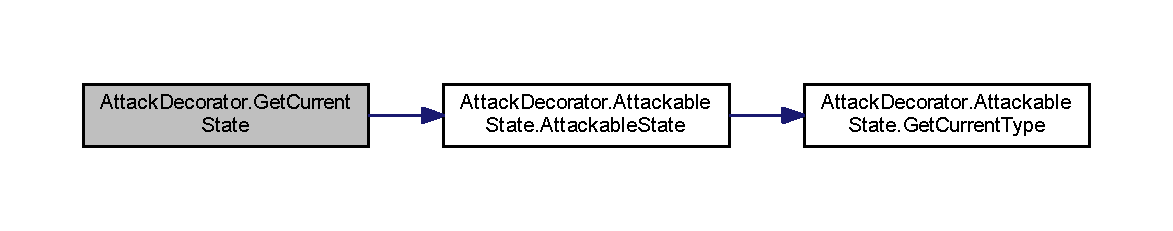
\includegraphics[width=350pt]{class_attack_decorator_af56bf418b8ba41fa9c7d8a697e39ce26_cgraph}
\end{center}
\end{figure}




이 함수를 호출하는 함수들에 대한 그래프입니다.\+:
\nopagebreak
\begin{figure}[H]
\begin{center}
\leavevmode
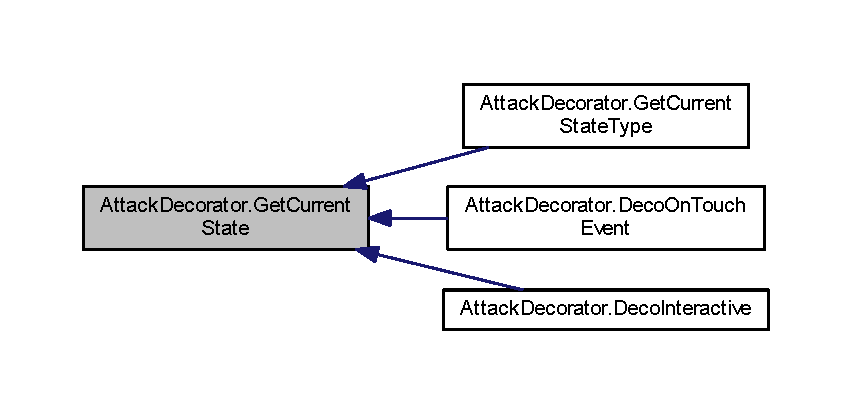
\includegraphics[width=350pt]{class_attack_decorator_af56bf418b8ba41fa9c7d8a697e39ce26_icgraph}
\end{center}
\end{figure}


\index{Attack\+Decorator@{Attack\+Decorator}!Get\+Current\+State\+Type@{Get\+Current\+State\+Type}}
\index{Get\+Current\+State\+Type@{Get\+Current\+State\+Type}!Attack\+Decorator@{Attack\+Decorator}}
\subsubsection[{\texorpdfstring{Get\+Current\+State\+Type()}{GetCurrentStateType()}}]{\setlength{\rightskip}{0pt plus 5cm}{\bf e\+Attackable\+Type} Attack\+Decorator.\+Get\+Current\+State\+Type (
\begin{DoxyParamCaption}
{}
\end{DoxyParamCaption}
)\hspace{0.3cm}{\ttfamily [private]}}\hypertarget{class_attack_decorator_a0fe90a081a8bf36c973b6a9b571c4966}{}\label{class_attack_decorator_a0fe90a081a8bf36c973b6a9b571c4966}


Attack\+Decorator.\+cs 파일의 100 번째 라인에서 정의되었습니다.


\begin{DoxyCode}
101     \{
102         var state = \hyperlink{class_attack_decorator_af56bf418b8ba41fa9c7d8a697e39ce26}{GetCurrentState}();
103 
104         \textcolor{keywordflow}{if} (state != null)
105         \{
106             \textcolor{keywordflow}{return} state.GetCurrentType();
107         \}
108 
109         \textcolor{keywordflow}{throw} \textcolor{keyword}{new} UnityException(\textcolor{stringliteral}{"don't have attackable state."});
110     \}
\end{DoxyCode}


이 함수 내부에서 호출하는 함수들에 대한 그래프입니다.\+:
\nopagebreak
\begin{figure}[H]
\begin{center}
\leavevmode
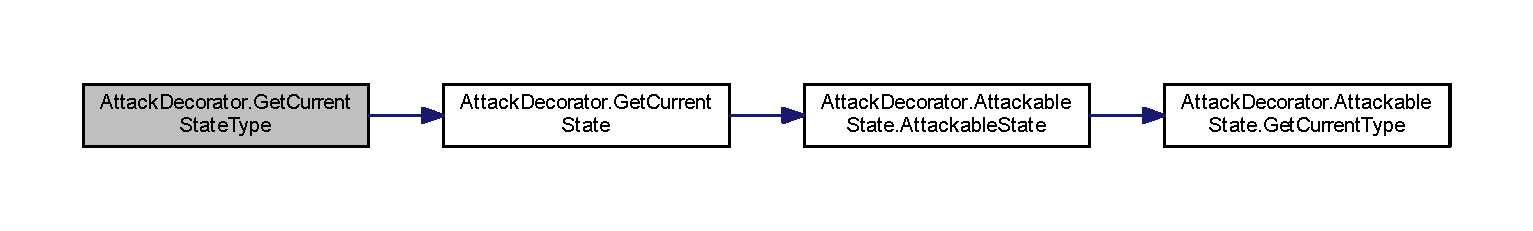
\includegraphics[width=350pt]{class_attack_decorator_a0fe90a081a8bf36c973b6a9b571c4966_cgraph}
\end{center}
\end{figure}


\index{Attack\+Decorator@{Attack\+Decorator}!Get\+Hash\+Code@{Get\+Hash\+Code}}
\index{Get\+Hash\+Code@{Get\+Hash\+Code}!Attack\+Decorator@{Attack\+Decorator}}
\subsubsection[{\texorpdfstring{Get\+Hash\+Code()}{GetHashCode()}}]{\setlength{\rightskip}{0pt plus 5cm}override int M\+C\+N.\+Decorator.\+Get\+Hash\+Code (
\begin{DoxyParamCaption}
{}
\end{DoxyParamCaption}
)\hspace{0.3cm}{\ttfamily [inherited]}}\hypertarget{class_m_c_n_1_1_decorator_a6df84cd2af5b096128e84791455c083f}{}\label{class_m_c_n_1_1_decorator_a6df84cd2af5b096128e84791455c083f}


Decorator.\+cs 파일의 249 번째 라인에서 정의되었습니다.


\begin{DoxyCode}
250         \{
251             \textcolor{keywordflow}{return} base.GetHashCode();
252         \}
\end{DoxyCode}
\index{Attack\+Decorator@{Attack\+Decorator}!Get\+Weight@{Get\+Weight}}
\index{Get\+Weight@{Get\+Weight}!Attack\+Decorator@{Attack\+Decorator}}
\subsubsection[{\texorpdfstring{Get\+Weight(string key)}{GetWeight(string key)}}]{\setlength{\rightskip}{0pt plus 5cm}int M\+C\+N.\+Decorator.\+Get\+Weight (
\begin{DoxyParamCaption}
\item[{string}]{key}
\end{DoxyParamCaption}
)\hspace{0.3cm}{\ttfamily [inherited]}}\hypertarget{class_m_c_n_1_1_decorator_a2fa8df5e51cc3fdaa63b28c4e4917670}{}\label{class_m_c_n_1_1_decorator_a2fa8df5e51cc3fdaa63b28c4e4917670}


Decorator.\+cs 파일의 168 번째 라인에서 정의되었습니다.


\begin{DoxyCode}
169         \{
170             \textcolor{keywordflow}{if}(\hyperlink{class_m_c_n_1_1_decorator_a1f9dd0c30a2fc261b7987d3ce36d8673}{\_weight}.ContainsKey(key))
171             \{
172                 \textcolor{keywordflow}{return} \hyperlink{class_m_c_n_1_1_decorator_a1f9dd0c30a2fc261b7987d3ce36d8673}{\_weight}[key];
173             \}
174 
175             \textcolor{keywordflow}{return} 0;
176         \}
\end{DoxyCode}
\index{Attack\+Decorator@{Attack\+Decorator}!Interactive@{Interactive}}
\index{Interactive@{Interactive}!Attack\+Decorator@{Attack\+Decorator}}
\subsubsection[{\texorpdfstring{Interactive(\+Tactics\+Object interact\+Target)}{Interactive(TacticsObject interactTarget)}}]{\setlength{\rightskip}{0pt plus 5cm}sealed override void M\+C\+N.\+Decorator.\+Interactive (
\begin{DoxyParamCaption}
\item[{{\bf Tactics\+Object}}]{interact\+Target}
\end{DoxyParamCaption}
)\hspace{0.3cm}{\ttfamily [virtual]}, {\ttfamily [inherited]}}\hypertarget{class_m_c_n_1_1_decorator_ae58cb79cf1ee47006b7dbdac82b97dc5}{}\label{class_m_c_n_1_1_decorator_ae58cb79cf1ee47006b7dbdac82b97dc5}


\hyperlink{class_tactics_object_a5f94ed01497a7072a2785163f4cbc57b}{Tactics\+Object}(으)로부터 재구현되었습니다.



Decorator.\+cs 파일의 265 번째 라인에서 정의되었습니다.


\begin{DoxyCode}
266         \{
267             base.Interactive(interactTarget);
268 
269             \hyperlink{class_m_c_n_1_1_decorator_a1ec6050ce16016f709aa8e8c19444678}{\_decoTarget}.\hyperlink{class_tactics_object_a5f94ed01497a7072a2785163f4cbc57b}{Interactive}(interactTarget);
270 
271             \hyperlink{class_m_c_n_1_1_decorator_a317f646a9053334fdbe28b9f1ae690a5}{DecoInteractive}(interactTarget);
272         \}
\end{DoxyCode}


이 함수 내부에서 호출하는 함수들에 대한 그래프입니다.\+:\nopagebreak
\begin{figure}[H]
\begin{center}
\leavevmode
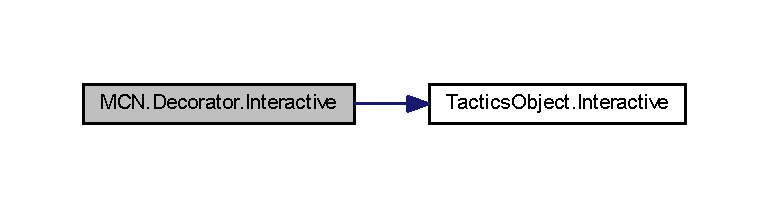
\includegraphics[width=350pt]{class_m_c_n_1_1_decorator_ae58cb79cf1ee47006b7dbdac82b97dc5_cgraph}
\end{center}
\end{figure}


\index{Attack\+Decorator@{Attack\+Decorator}!On\+Touch\+Event@{On\+Touch\+Event}}
\index{On\+Touch\+Event@{On\+Touch\+Event}!Attack\+Decorator@{Attack\+Decorator}}
\subsubsection[{\texorpdfstring{On\+Touch\+Event(e\+Touch\+Event touch)}{OnTouchEvent(eTouchEvent touch)}}]{\setlength{\rightskip}{0pt plus 5cm}sealed override bool M\+C\+N.\+Decorator.\+On\+Touch\+Event (
\begin{DoxyParamCaption}
\item[{{\bf e\+Touch\+Event}}]{touch}
\end{DoxyParamCaption}
)\hspace{0.3cm}{\ttfamily [virtual]}, {\ttfamily [inherited]}}\hypertarget{class_m_c_n_1_1_decorator_ac45ab12c190bd9f5188c9f748f8ddbbf}{}\label{class_m_c_n_1_1_decorator_ac45ab12c190bd9f5188c9f748f8ddbbf}


\hyperlink{class_tactics_object_af34052e62ea471d21e4c601cc79ff717}{Tactics\+Object}(으)로부터 재구현되었습니다.



Decorator.\+cs 파일의 255 번째 라인에서 정의되었습니다.


\begin{DoxyCode}
256         \{
257             base.OnTouchEvent(touch);
258 
259             \textcolor{comment}{// 만약 먼저 추가된 데코레이터의 touchEvent가 false를 반환한다면}
260             \textcolor{comment}{// 그 후에 추가된 데코레이터에는 터치 이벤트가 전달되지 않는다.}
261             \textcolor{keywordflow}{return} (\hyperlink{class_m_c_n_1_1_decorator_a1ec6050ce16016f709aa8e8c19444678}{\_decoTarget}.\hyperlink{class_tactics_object_af34052e62ea471d21e4c601cc79ff717}{OnTouchEvent}(touch) &&
262                     \hyperlink{class_m_c_n_1_1_decorator_abc499f6479fad929fc812e218d39a06d}{DecoOnTouchEvent}(touch));
263         \}
\end{DoxyCode}


이 함수 내부에서 호출하는 함수들에 대한 그래프입니다.\+:
\nopagebreak
\begin{figure}[H]
\begin{center}
\leavevmode
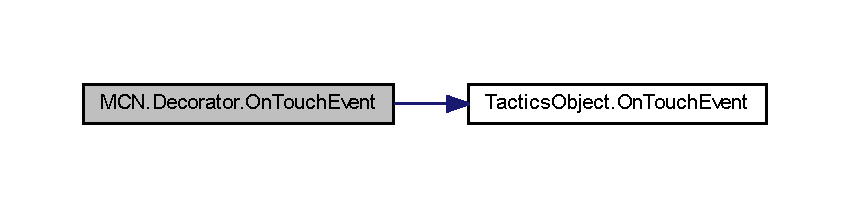
\includegraphics[width=350pt]{class_m_c_n_1_1_decorator_ac45ab12c190bd9f5188c9f748f8ddbbf_cgraph}
\end{center}
\end{figure}


\index{Attack\+Decorator@{Attack\+Decorator}!operator"!=@{operator"!=}}
\index{operator"!=@{operator"!=}!Attack\+Decorator@{Attack\+Decorator}}
\subsubsection[{\texorpdfstring{operator"!=(\+Tactics\+Object lt, Tactics\+Object rt)}{operator!=(TacticsObject lt, TacticsObject rt)}}]{\setlength{\rightskip}{0pt plus 5cm}static bool Tactics\+Object.\+operator!= (
\begin{DoxyParamCaption}
\item[{{\bf Tactics\+Object}}]{lt, }
\item[{{\bf Tactics\+Object}}]{rt}
\end{DoxyParamCaption}
)\hspace{0.3cm}{\ttfamily [static]}, {\ttfamily [inherited]}}\hypertarget{class_tactics_object_a49e235618a22126faa6271243cd89710}{}\label{class_tactics_object_a49e235618a22126faa6271243cd89710}


Tactics\+Object.\+cs 파일의 29 번째 라인에서 정의되었습니다.


\begin{DoxyCode}
30     \{
31         \textcolor{keywordflow}{return} !(rt == lt);
32     \}
\end{DoxyCode}
\index{Attack\+Decorator@{Attack\+Decorator}!operator"!=@{operator"!=}}
\index{operator"!=@{operator"!=}!Attack\+Decorator@{Attack\+Decorator}}
\subsubsection[{\texorpdfstring{operator"!=(\+Decoable lt, Decoable rt)}{operator!=(Decoable lt, Decoable rt)}}]{\setlength{\rightskip}{0pt plus 5cm}static bool M\+C\+N.\+Decoable.\+operator!= (
\begin{DoxyParamCaption}
\item[{{\bf Decoable}}]{lt, }
\item[{{\bf Decoable}}]{rt}
\end{DoxyParamCaption}
)\hspace{0.3cm}{\ttfamily [static]}, {\ttfamily [inherited]}}\hypertarget{class_m_c_n_1_1_decoable_aa75e4102ebd7265f577028b407534d27}{}\label{class_m_c_n_1_1_decoable_aa75e4102ebd7265f577028b407534d27}


Decorator.\+cs 파일의 36 번째 라인에서 정의되었습니다.


\begin{DoxyCode}
37         \{
38             \textcolor{keywordflow}{return} !(rt == lt);
39         \}
\end{DoxyCode}
\index{Attack\+Decorator@{Attack\+Decorator}!operator"!=@{operator"!=}}
\index{operator"!=@{operator"!=}!Attack\+Decorator@{Attack\+Decorator}}
\subsubsection[{\texorpdfstring{operator"!=(\+Decorator lt, Deco\+Instance rt)}{operator!=(Decorator lt, DecoInstance rt)}}]{\setlength{\rightskip}{0pt plus 5cm}static bool M\+C\+N.\+Decorator.\+operator!= (
\begin{DoxyParamCaption}
\item[{{\bf Decorator}}]{lt, }
\item[{{\bf Deco\+Instance}}]{rt}
\end{DoxyParamCaption}
)\hspace{0.3cm}{\ttfamily [static]}, {\ttfamily [inherited]}}\hypertarget{class_m_c_n_1_1_decorator_a89e2f61a0974c51610a0c8d14ef6962a}{}\label{class_m_c_n_1_1_decorator_a89e2f61a0974c51610a0c8d14ef6962a}


Decorator.\+cs 파일의 224 번째 라인에서 정의되었습니다.


\begin{DoxyCode}
225         \{
226             \textcolor{keywordflow}{return} !(rt == lt);
227         \}
\end{DoxyCode}
\index{Attack\+Decorator@{Attack\+Decorator}!operator==@{operator==}}
\index{operator==@{operator==}!Attack\+Decorator@{Attack\+Decorator}}
\subsubsection[{\texorpdfstring{operator==(\+Tactics\+Object lt, Tactics\+Object rt)}{operator==(TacticsObject lt, TacticsObject rt)}}]{\setlength{\rightskip}{0pt plus 5cm}static bool Tactics\+Object.\+operator== (
\begin{DoxyParamCaption}
\item[{{\bf Tactics\+Object}}]{lt, }
\item[{{\bf Tactics\+Object}}]{rt}
\end{DoxyParamCaption}
)\hspace{0.3cm}{\ttfamily [static]}, {\ttfamily [inherited]}}\hypertarget{class_tactics_object_a18f2979a4bf81dc755fbc17e425809f0}{}\label{class_tactics_object_a18f2979a4bf81dc755fbc17e425809f0}


Tactics\+Object.\+cs 파일의 9 번째 라인에서 정의되었습니다.


\begin{DoxyCode}
10     \{
11         \textcolor{keywordflow}{if} (\hyperlink{namespace_system}{System}.Object.ReferenceEquals(lt, rt))
12         \{
13             \textcolor{keywordflow}{return} \textcolor{keyword}{true};
14         \}
15 
16         \textcolor{keywordflow}{if} (((\textcolor{keywordtype}{object})lt == null) || ((object)rt == null))
17         \{
18             \textcolor{keywordflow}{return} \textcolor{keyword}{false};
19         \}
20 
21         \textcolor{keywordflow}{if} (lt is \hyperlink{namespace_m_c_n}{MCN}.\hyperlink{class_m_c_n_1_1_decoable}{Decoable} && rt is \hyperlink{namespace_m_c_n}{MCN}.\hyperlink{class_m_c_n_1_1_decoable}{Decoable})
22         \{
23             \textcolor{keywordflow}{return} (lt as \hyperlink{namespace_m_c_n}{MCN}.\hyperlink{class_m_c_n_1_1_decoable}{Decoable}) == (rt as \hyperlink{namespace_m_c_n}{MCN}.\hyperlink{class_m_c_n_1_1_decoable}{Decoable});
24         \}
25         
26         \textcolor{keywordflow}{return} (\textcolor{keywordtype}{object})lt == (object)rt;
27     \}
\end{DoxyCode}
\index{Attack\+Decorator@{Attack\+Decorator}!operator==@{operator==}}
\index{operator==@{operator==}!Attack\+Decorator@{Attack\+Decorator}}
\subsubsection[{\texorpdfstring{operator==(\+Decoable lt, Decoable rt)}{operator==(Decoable lt, Decoable rt)}}]{\setlength{\rightskip}{0pt plus 5cm}static bool M\+C\+N.\+Decoable.\+operator== (
\begin{DoxyParamCaption}
\item[{{\bf Decoable}}]{lt, }
\item[{{\bf Decoable}}]{rt}
\end{DoxyParamCaption}
)\hspace{0.3cm}{\ttfamily [static]}, {\ttfamily [inherited]}}\hypertarget{class_m_c_n_1_1_decoable_a6004bbc5f208c3031388c9d6e8f8359b}{}\label{class_m_c_n_1_1_decoable_a6004bbc5f208c3031388c9d6e8f8359b}


Decorator.\+cs 파일의 11 번째 라인에서 정의되었습니다.


\begin{DoxyCode}
12         \{
13             \textcolor{keywordflow}{if} (\hyperlink{namespace_system}{System}.Object.ReferenceEquals(lt, rt))
14             \{
15                 \textcolor{keywordflow}{return} \textcolor{keyword}{true};
16             \}
17 
18             \textcolor{keywordflow}{if} (((\textcolor{keywordtype}{object})lt == null) || ((object)rt == null))
19             \{
20                 \textcolor{keywordflow}{return} \textcolor{keyword}{false};
21             \}
22             
23             \textcolor{keywordflow}{if}(lt is DecoInstance && rt is Decorator)
24             \{
25                 \textcolor{keywordflow}{return} (lt as DecoInstance) == (rt as Decorator);
26             \}
27 
28             \textcolor{keywordflow}{if} (rt is DecoInstance && lt is Decorator)
29             \{
30                 \textcolor{keywordflow}{return} (rt as DecoInstance) == (lt as Decorator);
31             \}
32 
33             \textcolor{keywordflow}{return} (\textcolor{keywordtype}{object})lt == (object)rt;
34         \}
\end{DoxyCode}
\index{Attack\+Decorator@{Attack\+Decorator}!operator==@{operator==}}
\index{operator==@{operator==}!Attack\+Decorator@{Attack\+Decorator}}
\subsubsection[{\texorpdfstring{operator==(\+Decorator lt, Deco\+Instance rt)}{operator==(Decorator lt, DecoInstance rt)}}]{\setlength{\rightskip}{0pt plus 5cm}static bool M\+C\+N.\+Decorator.\+operator== (
\begin{DoxyParamCaption}
\item[{{\bf Decorator}}]{lt, }
\item[{{\bf Deco\+Instance}}]{rt}
\end{DoxyParamCaption}
)\hspace{0.3cm}{\ttfamily [static]}, {\ttfamily [inherited]}}\hypertarget{class_m_c_n_1_1_decorator_a4c4c97e4a4dcf1a66e764740a5bbf3c6}{}\label{class_m_c_n_1_1_decorator_a4c4c97e4a4dcf1a66e764740a5bbf3c6}


Decorator.\+cs 파일의 209 번째 라인에서 정의되었습니다.


\begin{DoxyCode}
210         \{
211             \textcolor{keywordflow}{if} (\hyperlink{namespace_system}{System}.Object.ReferenceEquals(lt, rt))
212             \{
213                 \textcolor{keywordflow}{return} \textcolor{keyword}{true};
214             \}
215 
216             \textcolor{keywordflow}{if} (((\textcolor{keywordtype}{object})lt == null) || ((object)rt == null))
217             \{
218                 \textcolor{keywordflow}{return} \textcolor{keyword}{false};
219             \}
220 
221             \textcolor{keywordflow}{return} lt.DecoTarget == rt;
222         \}
\end{DoxyCode}
\index{Attack\+Decorator@{Attack\+Decorator}!Set\+Weight@{Set\+Weight}}
\index{Set\+Weight@{Set\+Weight}!Attack\+Decorator@{Attack\+Decorator}}
\subsubsection[{\texorpdfstring{Set\+Weight(string key, int weight)}{SetWeight(string key, int weight)}}]{\setlength{\rightskip}{0pt plus 5cm}void M\+C\+N.\+Decorator.\+Set\+Weight (
\begin{DoxyParamCaption}
\item[{string}]{key, }
\item[{int}]{weight}
\end{DoxyParamCaption}
)\hspace{0.3cm}{\ttfamily [inherited]}}\hypertarget{class_m_c_n_1_1_decorator_a0658f2776c28dad0517b56085910162c}{}\label{class_m_c_n_1_1_decorator_a0658f2776c28dad0517b56085910162c}


Decorator.\+cs 파일의 178 번째 라인에서 정의되었습니다.


\begin{DoxyCode}
179         \{
180             \hyperlink{class_m_c_n_1_1_decorator_a1f9dd0c30a2fc261b7987d3ce36d8673}{\_weight}[key] = weight;
181         \}
\end{DoxyCode}
\index{Attack\+Decorator@{Attack\+Decorator}!Set\+Weight@{Set\+Weight}}
\index{Set\+Weight@{Set\+Weight}!Attack\+Decorator@{Attack\+Decorator}}
\subsubsection[{\texorpdfstring{Set\+Weight(\+Pair$<$ string, int $>$ info)}{SetWeight(Pair< string, int > info)}}]{\setlength{\rightskip}{0pt plus 5cm}void M\+C\+N.\+Decorator.\+Set\+Weight (
\begin{DoxyParamCaption}
\item[{{\bf Pair}$<$ string, int $>$}]{info}
\end{DoxyParamCaption}
)\hspace{0.3cm}{\ttfamily [inherited]}}\hypertarget{class_m_c_n_1_1_decorator_aa64c6b8a8f30f4e8083da6dd0fab226c}{}\label{class_m_c_n_1_1_decorator_aa64c6b8a8f30f4e8083da6dd0fab226c}


Decorator.\+cs 파일의 183 번째 라인에서 정의되었습니다.


\begin{DoxyCode}
184         \{
185             \textcolor{keywordflow}{if}(info != null)
186             \{
187                 \textcolor{keywordflow}{if}(\hyperlink{class_m_c_n_1_1_decorator_a1f9dd0c30a2fc261b7987d3ce36d8673}{\_weight} == null)
188                 \{
189                     \hyperlink{class_m_c_n_1_1_decorator_a1f9dd0c30a2fc261b7987d3ce36d8673}{\_weight} = \textcolor{keyword}{new} Dictionary<string, int>();
190                 \}
191 
192                 \hyperlink{class_m_c_n_1_1_decorator_a1f9dd0c30a2fc261b7987d3ce36d8673}{\_weight}[info.\hyperlink{class_m_c_n_1_1_pair_a62c546d3829b8819a65f8c9d64200338}{key}] = info.\hyperlink{class_m_c_n_1_1_pair_a1980bbf37b60fcbfea22382f71250e84}{value};
193             \}
194         \}
\end{DoxyCode}
\index{Attack\+Decorator@{Attack\+Decorator}!Storage\+States@{Storage\+States}}
\index{Storage\+States@{Storage\+States}!Attack\+Decorator@{Attack\+Decorator}}
\subsubsection[{\texorpdfstring{Storage\+States()}{StorageStates()}}]{\setlength{\rightskip}{0pt plus 5cm}void Attack\+Decorator.\+Storage\+States (
\begin{DoxyParamCaption}
{}
\end{DoxyParamCaption}
)\hspace{0.3cm}{\ttfamily [private]}}\hypertarget{class_attack_decorator_a4c5bb156eda734c19594c740c6d63aad}{}\label{class_attack_decorator_a4c5bb156eda734c19594c740c6d63aad}


Attack\+Decorator.\+cs 파일의 84 번째 라인에서 정의되었습니다.


\begin{DoxyCode}
85     \{
86         \textcolor{comment}{// TODO : 스테이트들을 적재한다.}
87     \}
\end{DoxyCode}


이 함수를 호출하는 함수들에 대한 그래프입니다.\+:
\nopagebreak
\begin{figure}[H]
\begin{center}
\leavevmode
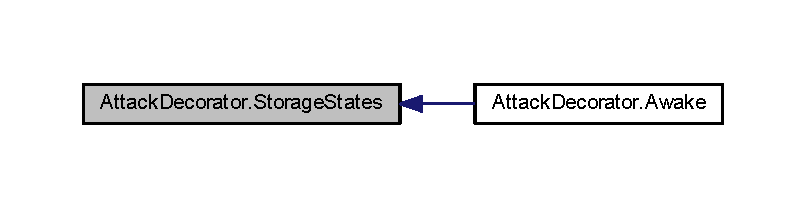
\includegraphics[width=350pt]{class_attack_decorator_a4c5bb156eda734c19594c740c6d63aad_icgraph}
\end{center}
\end{figure}




\subsection{멤버 데이타 문서화}
\index{Attack\+Decorator@{Attack\+Decorator}!\+\_\+attackable\+State\+Machine@{\+\_\+attackable\+State\+Machine}}
\index{\+\_\+attackable\+State\+Machine@{\+\_\+attackable\+State\+Machine}!Attack\+Decorator@{Attack\+Decorator}}
\subsubsection[{\texorpdfstring{\+\_\+attackable\+State\+Machine}{_attackableStateMachine}}]{\setlength{\rightskip}{0pt plus 5cm}{\bf M\+C\+N.\+State\+Machine}$<${\bf Attackable\+State}$>$ Attack\+Decorator.\+\_\+attackable\+State\+Machine = new {\bf M\+C\+N.\+State\+Machine}$<${\bf Attackable\+State}$>$()\hspace{0.3cm}{\ttfamily [private]}}\hypertarget{class_attack_decorator_a0ddeffefa8d7bce11d4681c07c50183c}{}\label{class_attack_decorator_a0ddeffefa8d7bce11d4681c07c50183c}


Attack\+Decorator.\+cs 파일의 38 번째 라인에서 정의되었습니다.



\subsection{속성 문서화}
\index{Attack\+Decorator@{Attack\+Decorator}!Deco\+Target@{Deco\+Target}}
\index{Deco\+Target@{Deco\+Target}!Attack\+Decorator@{Attack\+Decorator}}
\subsubsection[{\texorpdfstring{Deco\+Target}{DecoTarget}}]{\setlength{\rightskip}{0pt plus 5cm}{\bf M\+C\+N.\+Decoable} M\+C\+N.\+Decorator.\+Deco\+Target\hspace{0.3cm}{\ttfamily [get]}, {\ttfamily [protected]}, {\ttfamily [inherited]}}\hypertarget{class_m_c_n_1_1_decorator_a1306a0a8b814650cd5970a1ffc7ba2fe}{}\label{class_m_c_n_1_1_decorator_a1306a0a8b814650cd5970a1ffc7ba2fe}


Decorator.\+cs 파일의 145 번째 라인에서 정의되었습니다.

\index{Attack\+Decorator@{Attack\+Decorator}!Power@{Power}}
\index{Power@{Power}!Attack\+Decorator@{Attack\+Decorator}}
\subsubsection[{\texorpdfstring{Power}{Power}}]{\setlength{\rightskip}{0pt plus 5cm}int Attack\+Decorator.\+Power\hspace{0.3cm}{\ttfamily [get]}, {\ttfamily [private]}}\hypertarget{class_attack_decorator_a3305d359c9c0faaf4f12aa261492ee7c}{}\label{class_attack_decorator_a3305d359c9c0faaf4f12aa261492ee7c}


Attack\+Decorator.\+cs 파일의 24 번째 라인에서 정의되었습니다.

\index{Attack\+Decorator@{Attack\+Decorator}!Range@{Range}}
\index{Range@{Range}!Attack\+Decorator@{Attack\+Decorator}}
\subsubsection[{\texorpdfstring{Range}{Range}}]{\setlength{\rightskip}{0pt plus 5cm}int Attack\+Decorator.\+Range\hspace{0.3cm}{\ttfamily [get]}, {\ttfamily [private]}}\hypertarget{class_attack_decorator_ad025c4d20cc5dba4326ecbd52562a3c4}{}\label{class_attack_decorator_ad025c4d20cc5dba4326ecbd52562a3c4}


Attack\+Decorator.\+cs 파일의 16 번째 라인에서 정의되었습니다.



이 클래스에 대한 문서화 페이지는 다음의 파일로부터 생성되었습니다.\+:\begin{DoxyCompactItemize}
\item 
D\+:/\+Git\+Hub/\+M\+C\+N\+Tactics/\+Assets/\+Scripts/\+Objects/\+Decorator/\hyperlink{_attack_decorator_8cs}{Attack\+Decorator.\+cs}\end{DoxyCompactItemize}

\hypertarget{class_m_c_n_1_1_decoable}{}\section{M\+C\+N.\+Decoable 클래스 참조}
\label{class_m_c_n_1_1_decoable}\index{M\+C\+N.\+Decoable@{M\+C\+N.\+Decoable}}


M\+C\+N.\+Decoable에 대한 상속 다이어그램 \+: 
\nopagebreak
\begin{figure}[H]
\begin{center}
\leavevmode
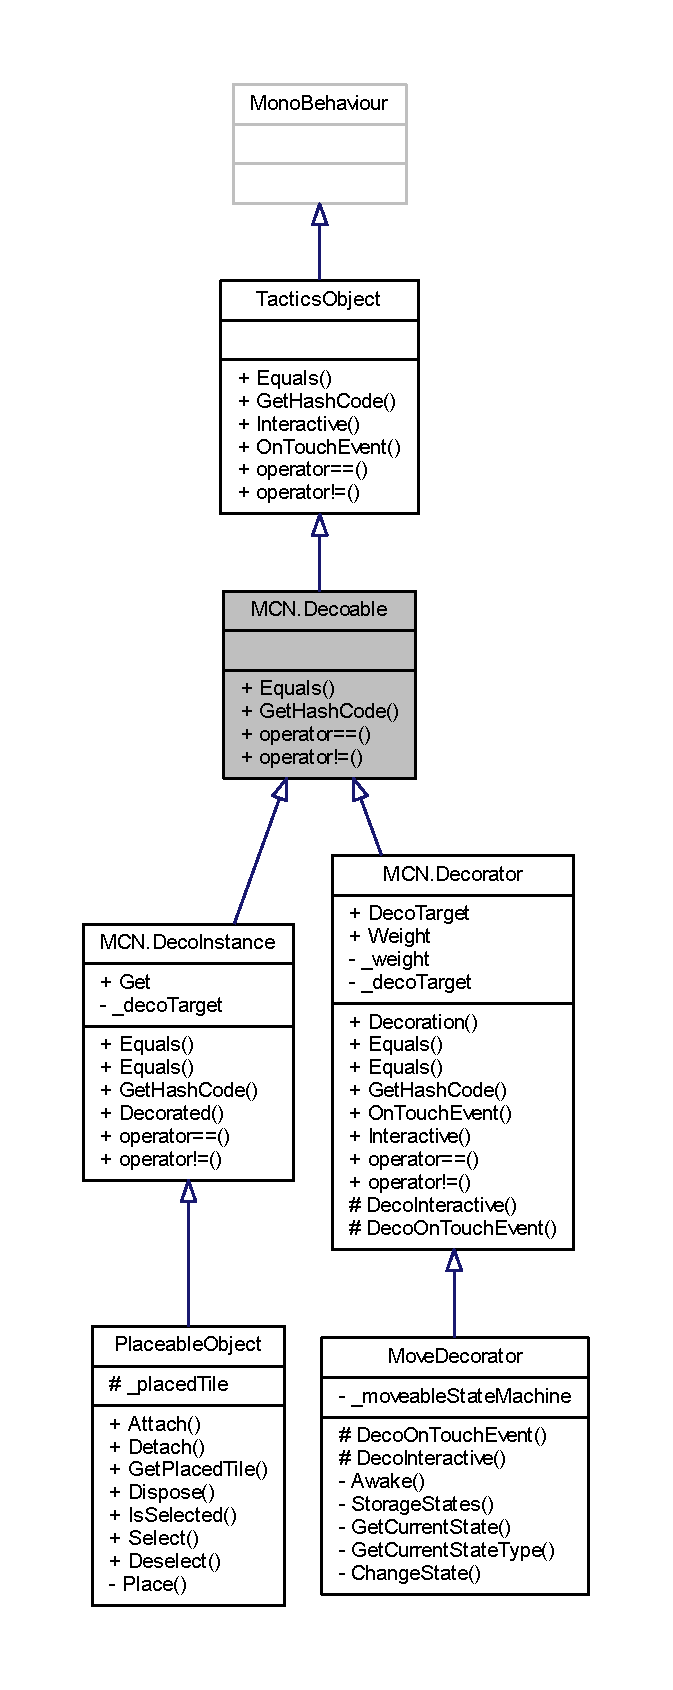
\includegraphics[height=550pt]{class_m_c_n_1_1_decoable__inherit__graph}
\end{center}
\end{figure}


M\+C\+N.\+Decoable에 대한 협력 다이어그램\+:\nopagebreak
\begin{figure}[H]
\begin{center}
\leavevmode
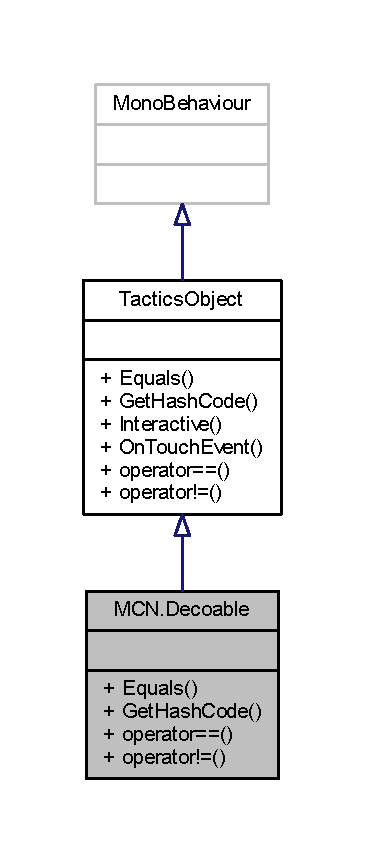
\includegraphics[width=175pt]{class_m_c_n_1_1_decoable__coll__graph}
\end{center}
\end{figure}
\subsection*{Public 멤버 함수}
\begin{DoxyCompactItemize}
\item 
override bool \hyperlink{class_m_c_n_1_1_decoable_a7c14e3879800d1f5d7e58a02e75540d9}{Equals} (object o)
\item 
override int \hyperlink{class_m_c_n_1_1_decoable_ad3068f4dce16b691595d54bb2f7a2d5c}{Get\+Hash\+Code} ()
\item 
virtual void \hyperlink{class_tactics_object_a5f94ed01497a7072a2785163f4cbc57b}{Interactive} (\hyperlink{class_tactics_object}{Tactics\+Object} interact\+Target)
\item 
virtual bool \hyperlink{class_tactics_object_af34052e62ea471d21e4c601cc79ff717}{On\+Touch\+Event} (\hyperlink{_touch_manager_8cs_ae33e321a424fe84ba8b2fdb81ad40a68}{e\+Touch\+Event} touch)
\end{DoxyCompactItemize}
\subsection*{정적 Public 멤버 함수}
\begin{DoxyCompactItemize}
\item 
static bool \hyperlink{class_m_c_n_1_1_decoable_a6004bbc5f208c3031388c9d6e8f8359b}{operator==} (\hyperlink{class_m_c_n_1_1_decoable}{Decoable} lt, \hyperlink{class_m_c_n_1_1_decoable}{Decoable} rt)
\item 
static bool \hyperlink{class_m_c_n_1_1_decoable_aa75e4102ebd7265f577028b407534d27}{operator!=} (\hyperlink{class_m_c_n_1_1_decoable}{Decoable} lt, \hyperlink{class_m_c_n_1_1_decoable}{Decoable} rt)
\item 
static bool \hyperlink{class_tactics_object_a18f2979a4bf81dc755fbc17e425809f0}{operator==} (\hyperlink{class_tactics_object}{Tactics\+Object} lt, \hyperlink{class_tactics_object}{Tactics\+Object} rt)
\item 
static bool \hyperlink{class_tactics_object_a49e235618a22126faa6271243cd89710}{operator!=} (\hyperlink{class_tactics_object}{Tactics\+Object} lt, \hyperlink{class_tactics_object}{Tactics\+Object} rt)
\end{DoxyCompactItemize}


\subsection{상세한 설명}


Decorator.\+cs 파일의 7 번째 라인에서 정의되었습니다.



\subsection{멤버 함수 문서화}
\index{M\+C\+N\+::\+Decoable@{M\+C\+N\+::\+Decoable}!Equals@{Equals}}
\index{Equals@{Equals}!M\+C\+N\+::\+Decoable@{M\+C\+N\+::\+Decoable}}
\subsubsection[{\texorpdfstring{Equals(object o)}{Equals(object o)}}]{\setlength{\rightskip}{0pt plus 5cm}override bool M\+C\+N.\+Decoable.\+Equals (
\begin{DoxyParamCaption}
\item[{object}]{o}
\end{DoxyParamCaption}
)}\hypertarget{class_m_c_n_1_1_decoable_a7c14e3879800d1f5d7e58a02e75540d9}{}\label{class_m_c_n_1_1_decoable_a7c14e3879800d1f5d7e58a02e75540d9}


Decorator.\+cs 파일의 41 번째 라인에서 정의되었습니다.


\begin{DoxyCode}
42         \{
43             \textcolor{keywordflow}{if} (\textcolor{keyword}{this} is DecoInstance)
44             \{
45                 (\textcolor{keyword}{this} as DecoInstance).\hyperlink{class_m_c_n_1_1_decoable_a7c14e3879800d1f5d7e58a02e75540d9}{Equals}(o);
46             \}
47 
48             \textcolor{keywordflow}{if}(\textcolor{keyword}{this} is Decorator)
49             \{
50                 (\textcolor{keyword}{this} as Decorator).\hyperlink{class_m_c_n_1_1_decoable_a7c14e3879800d1f5d7e58a02e75540d9}{Equals}(o);
51             \}
52 
53             \textcolor{keywordflow}{return} base.Equals(o);
54         \}
\end{DoxyCode}


이 함수를 호출하는 함수들에 대한 그래프입니다.\+:\nopagebreak
\begin{figure}[H]
\begin{center}
\leavevmode
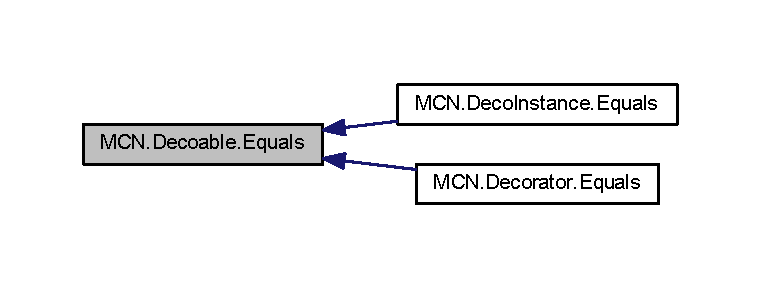
\includegraphics[width=350pt]{class_m_c_n_1_1_decoable_a7c14e3879800d1f5d7e58a02e75540d9_icgraph}
\end{center}
\end{figure}


\index{M\+C\+N\+::\+Decoable@{M\+C\+N\+::\+Decoable}!Get\+Hash\+Code@{Get\+Hash\+Code}}
\index{Get\+Hash\+Code@{Get\+Hash\+Code}!M\+C\+N\+::\+Decoable@{M\+C\+N\+::\+Decoable}}
\subsubsection[{\texorpdfstring{Get\+Hash\+Code()}{GetHashCode()}}]{\setlength{\rightskip}{0pt plus 5cm}override int M\+C\+N.\+Decoable.\+Get\+Hash\+Code (
\begin{DoxyParamCaption}
{}
\end{DoxyParamCaption}
)}\hypertarget{class_m_c_n_1_1_decoable_ad3068f4dce16b691595d54bb2f7a2d5c}{}\label{class_m_c_n_1_1_decoable_ad3068f4dce16b691595d54bb2f7a2d5c}


Decorator.\+cs 파일의 56 번째 라인에서 정의되었습니다.


\begin{DoxyCode}
57         \{
58             \textcolor{keywordflow}{return} base.GetHashCode();
59         \}
\end{DoxyCode}
\index{M\+C\+N\+::\+Decoable@{M\+C\+N\+::\+Decoable}!Interactive@{Interactive}}
\index{Interactive@{Interactive}!M\+C\+N\+::\+Decoable@{M\+C\+N\+::\+Decoable}}
\subsubsection[{\texorpdfstring{Interactive(\+Tactics\+Object interact\+Target)}{Interactive(TacticsObject interactTarget)}}]{\setlength{\rightskip}{0pt plus 5cm}virtual void Tactics\+Object.\+Interactive (
\begin{DoxyParamCaption}
\item[{{\bf Tactics\+Object}}]{interact\+Target}
\end{DoxyParamCaption}
)\hspace{0.3cm}{\ttfamily [virtual]}, {\ttfamily [inherited]}}\hypertarget{class_tactics_object_a5f94ed01497a7072a2785163f4cbc57b}{}\label{class_tactics_object_a5f94ed01497a7072a2785163f4cbc57b}


\hyperlink{class_m_c_n_1_1_decorator_ae58cb79cf1ee47006b7dbdac82b97dc5}{M\+C\+N.\+Decorator}에서 재구현되었습니다.



Tactics\+Object.\+cs 파일의 50 번째 라인에서 정의되었습니다.


\begin{DoxyCode}
50 \{ \}
\end{DoxyCode}


이 함수를 호출하는 함수들에 대한 그래프입니다.\+:\nopagebreak
\begin{figure}[H]
\begin{center}
\leavevmode
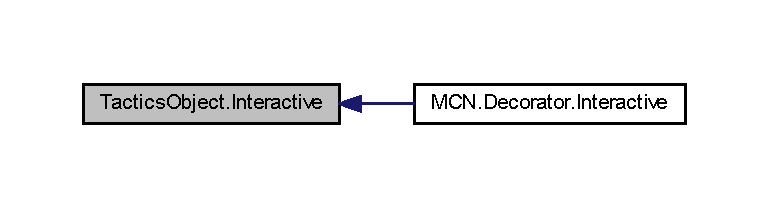
\includegraphics[width=350pt]{class_tactics_object_a5f94ed01497a7072a2785163f4cbc57b_icgraph}
\end{center}
\end{figure}


\index{M\+C\+N\+::\+Decoable@{M\+C\+N\+::\+Decoable}!On\+Touch\+Event@{On\+Touch\+Event}}
\index{On\+Touch\+Event@{On\+Touch\+Event}!M\+C\+N\+::\+Decoable@{M\+C\+N\+::\+Decoable}}
\subsubsection[{\texorpdfstring{On\+Touch\+Event(e\+Touch\+Event touch)}{OnTouchEvent(eTouchEvent touch)}}]{\setlength{\rightskip}{0pt plus 5cm}virtual bool Tactics\+Object.\+On\+Touch\+Event (
\begin{DoxyParamCaption}
\item[{{\bf e\+Touch\+Event}}]{touch}
\end{DoxyParamCaption}
)\hspace{0.3cm}{\ttfamily [virtual]}, {\ttfamily [inherited]}}\hypertarget{class_tactics_object_af34052e62ea471d21e4c601cc79ff717}{}\label{class_tactics_object_af34052e62ea471d21e4c601cc79ff717}


\hyperlink{class_m_c_n_1_1_decorator_ac45ab12c190bd9f5188c9f748f8ddbbf}{M\+C\+N.\+Decorator}에서 재구현되었습니다.



Tactics\+Object.\+cs 파일의 52 번째 라인에서 정의되었습니다.


\begin{DoxyCode}
52 \{ \textcolor{keywordflow}{return} \textcolor{keyword}{true}; \}
\end{DoxyCode}


이 함수를 호출하는 함수들에 대한 그래프입니다.\+:
\nopagebreak
\begin{figure}[H]
\begin{center}
\leavevmode
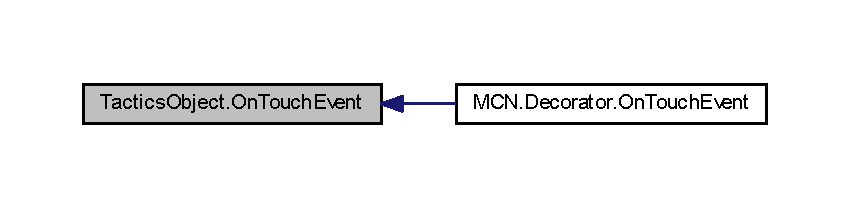
\includegraphics[width=350pt]{class_tactics_object_af34052e62ea471d21e4c601cc79ff717_icgraph}
\end{center}
\end{figure}


\index{M\+C\+N\+::\+Decoable@{M\+C\+N\+::\+Decoable}!operator"!=@{operator"!=}}
\index{operator"!=@{operator"!=}!M\+C\+N\+::\+Decoable@{M\+C\+N\+::\+Decoable}}
\subsubsection[{\texorpdfstring{operator"!=(\+Tactics\+Object lt, Tactics\+Object rt)}{operator!=(TacticsObject lt, TacticsObject rt)}}]{\setlength{\rightskip}{0pt plus 5cm}static bool Tactics\+Object.\+operator!= (
\begin{DoxyParamCaption}
\item[{{\bf Tactics\+Object}}]{lt, }
\item[{{\bf Tactics\+Object}}]{rt}
\end{DoxyParamCaption}
)\hspace{0.3cm}{\ttfamily [static]}, {\ttfamily [inherited]}}\hypertarget{class_tactics_object_a49e235618a22126faa6271243cd89710}{}\label{class_tactics_object_a49e235618a22126faa6271243cd89710}


Tactics\+Object.\+cs 파일의 29 번째 라인에서 정의되었습니다.


\begin{DoxyCode}
30     \{
31         \textcolor{keywordflow}{return} !(rt == lt);
32     \}
\end{DoxyCode}
\index{M\+C\+N\+::\+Decoable@{M\+C\+N\+::\+Decoable}!operator"!=@{operator"!=}}
\index{operator"!=@{operator"!=}!M\+C\+N\+::\+Decoable@{M\+C\+N\+::\+Decoable}}
\subsubsection[{\texorpdfstring{operator"!=(\+Decoable lt, Decoable rt)}{operator!=(Decoable lt, Decoable rt)}}]{\setlength{\rightskip}{0pt plus 5cm}static bool M\+C\+N.\+Decoable.\+operator!= (
\begin{DoxyParamCaption}
\item[{{\bf Decoable}}]{lt, }
\item[{{\bf Decoable}}]{rt}
\end{DoxyParamCaption}
)\hspace{0.3cm}{\ttfamily [static]}}\hypertarget{class_m_c_n_1_1_decoable_aa75e4102ebd7265f577028b407534d27}{}\label{class_m_c_n_1_1_decoable_aa75e4102ebd7265f577028b407534d27}


Decorator.\+cs 파일의 36 번째 라인에서 정의되었습니다.


\begin{DoxyCode}
37         \{
38             \textcolor{keywordflow}{return} !(rt == lt);
39         \}
\end{DoxyCode}
\index{M\+C\+N\+::\+Decoable@{M\+C\+N\+::\+Decoable}!operator==@{operator==}}
\index{operator==@{operator==}!M\+C\+N\+::\+Decoable@{M\+C\+N\+::\+Decoable}}
\subsubsection[{\texorpdfstring{operator==(\+Tactics\+Object lt, Tactics\+Object rt)}{operator==(TacticsObject lt, TacticsObject rt)}}]{\setlength{\rightskip}{0pt plus 5cm}static bool Tactics\+Object.\+operator== (
\begin{DoxyParamCaption}
\item[{{\bf Tactics\+Object}}]{lt, }
\item[{{\bf Tactics\+Object}}]{rt}
\end{DoxyParamCaption}
)\hspace{0.3cm}{\ttfamily [static]}, {\ttfamily [inherited]}}\hypertarget{class_tactics_object_a18f2979a4bf81dc755fbc17e425809f0}{}\label{class_tactics_object_a18f2979a4bf81dc755fbc17e425809f0}


Tactics\+Object.\+cs 파일의 9 번째 라인에서 정의되었습니다.


\begin{DoxyCode}
10     \{
11         \textcolor{keywordflow}{if} (\hyperlink{namespace_system}{System}.Object.ReferenceEquals(lt, rt))
12         \{
13             \textcolor{keywordflow}{return} \textcolor{keyword}{true};
14         \}
15 
16         \textcolor{keywordflow}{if} (((\textcolor{keywordtype}{object})lt == null) || ((object)rt == null))
17         \{
18             \textcolor{keywordflow}{return} \textcolor{keyword}{false};
19         \}
20 
21         \textcolor{keywordflow}{if} (lt is \hyperlink{namespace_m_c_n}{MCN}.\hyperlink{class_m_c_n_1_1_decoable}{Decoable} && rt is \hyperlink{namespace_m_c_n}{MCN}.\hyperlink{class_m_c_n_1_1_decoable}{Decoable})
22         \{
23             \textcolor{keywordflow}{return} (lt as \hyperlink{namespace_m_c_n}{MCN}.\hyperlink{class_m_c_n_1_1_decoable}{Decoable}) == (rt as \hyperlink{namespace_m_c_n}{MCN}.\hyperlink{class_m_c_n_1_1_decoable}{Decoable});
24         \}
25         
26         \textcolor{keywordflow}{return} (\textcolor{keywordtype}{object})lt == (object)rt;
27     \}
\end{DoxyCode}
\index{M\+C\+N\+::\+Decoable@{M\+C\+N\+::\+Decoable}!operator==@{operator==}}
\index{operator==@{operator==}!M\+C\+N\+::\+Decoable@{M\+C\+N\+::\+Decoable}}
\subsubsection[{\texorpdfstring{operator==(\+Decoable lt, Decoable rt)}{operator==(Decoable lt, Decoable rt)}}]{\setlength{\rightskip}{0pt plus 5cm}static bool M\+C\+N.\+Decoable.\+operator== (
\begin{DoxyParamCaption}
\item[{{\bf Decoable}}]{lt, }
\item[{{\bf Decoable}}]{rt}
\end{DoxyParamCaption}
)\hspace{0.3cm}{\ttfamily [static]}}\hypertarget{class_m_c_n_1_1_decoable_a6004bbc5f208c3031388c9d6e8f8359b}{}\label{class_m_c_n_1_1_decoable_a6004bbc5f208c3031388c9d6e8f8359b}


Decorator.\+cs 파일의 11 번째 라인에서 정의되었습니다.


\begin{DoxyCode}
12         \{
13             \textcolor{keywordflow}{if} (\hyperlink{namespace_system}{System}.Object.ReferenceEquals(lt, rt))
14             \{
15                 \textcolor{keywordflow}{return} \textcolor{keyword}{true};
16             \}
17 
18             \textcolor{keywordflow}{if} (((\textcolor{keywordtype}{object})lt == null) || ((object)rt == null))
19             \{
20                 \textcolor{keywordflow}{return} \textcolor{keyword}{false};
21             \}
22             
23             \textcolor{keywordflow}{if}(lt is DecoInstance && rt is Decorator)
24             \{
25                 \textcolor{keywordflow}{return} (lt as DecoInstance) == (rt as Decorator);
26             \}
27 
28             \textcolor{keywordflow}{if} (rt is DecoInstance && lt is Decorator)
29             \{
30                 \textcolor{keywordflow}{return} (rt as DecoInstance) == (lt as Decorator);
31             \}
32 
33             \textcolor{keywordflow}{return} (\textcolor{keywordtype}{object})lt == (object)rt;
34         \}
\end{DoxyCode}


이 클래스에 대한 문서화 페이지는 다음의 파일로부터 생성되었습니다.\+:\begin{DoxyCompactItemize}
\item 
D\+:/\+Git\+Hub/\+M\+C\+N\+Tactics/\+Assets/\+Scripts/\+Core/\hyperlink{_decorator_8cs}{Decorator.\+cs}\end{DoxyCompactItemize}

\hypertarget{class_m_c_n_1_1_deco_class_info}{}\section{M\+C\+N.\+Deco\+Class\+Info 클래스 참조}
\label{class_m_c_n_1_1_deco_class_info}\index{M\+C\+N.\+Deco\+Class\+Info@{M\+C\+N.\+Deco\+Class\+Info}}


M\+C\+N.\+Deco\+Class\+Info에 대한 협력 다이어그램\+:
\nopagebreak
\begin{figure}[H]
\begin{center}
\leavevmode
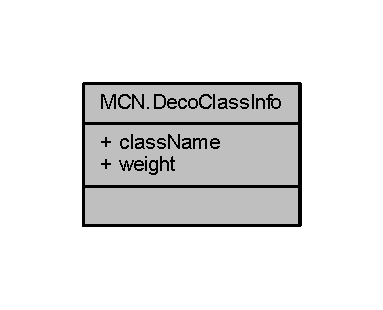
\includegraphics[width=184pt]{class_m_c_n_1_1_deco_class_info__coll__graph}
\end{center}
\end{figure}
\subsection*{Public 속성}
\begin{DoxyCompactItemize}
\item 
string \hyperlink{class_m_c_n_1_1_deco_class_info_a3b0fc8a06269e57ded3835ea02026859}{class\+Name}
\item 
List$<$ \hyperlink{class_m_c_n_1_1_string_int_pair}{String\+Int\+Pair} $>$ \hyperlink{class_m_c_n_1_1_deco_class_info_a04ed1d8d36502303fa7a2a1f872f1681}{weight}
\end{DoxyCompactItemize}


\subsection{상세한 설명}


Structure.\+cs 파일의 16 번째 라인에서 정의되었습니다.



\subsection{멤버 데이타 문서화}
\index{M\+C\+N\+::\+Deco\+Class\+Info@{M\+C\+N\+::\+Deco\+Class\+Info}!class\+Name@{class\+Name}}
\index{class\+Name@{class\+Name}!M\+C\+N\+::\+Deco\+Class\+Info@{M\+C\+N\+::\+Deco\+Class\+Info}}
\subsubsection[{\texorpdfstring{class\+Name}{className}}]{\setlength{\rightskip}{0pt plus 5cm}string M\+C\+N.\+Deco\+Class\+Info.\+class\+Name}\hypertarget{class_m_c_n_1_1_deco_class_info_a3b0fc8a06269e57ded3835ea02026859}{}\label{class_m_c_n_1_1_deco_class_info_a3b0fc8a06269e57ded3835ea02026859}


Structure.\+cs 파일의 18 번째 라인에서 정의되었습니다.

\index{M\+C\+N\+::\+Deco\+Class\+Info@{M\+C\+N\+::\+Deco\+Class\+Info}!weight@{weight}}
\index{weight@{weight}!M\+C\+N\+::\+Deco\+Class\+Info@{M\+C\+N\+::\+Deco\+Class\+Info}}
\subsubsection[{\texorpdfstring{weight}{weight}}]{\setlength{\rightskip}{0pt plus 5cm}List$<${\bf String\+Int\+Pair}$>$ M\+C\+N.\+Deco\+Class\+Info.\+weight}\hypertarget{class_m_c_n_1_1_deco_class_info_a04ed1d8d36502303fa7a2a1f872f1681}{}\label{class_m_c_n_1_1_deco_class_info_a04ed1d8d36502303fa7a2a1f872f1681}


Structure.\+cs 파일의 19 번째 라인에서 정의되었습니다.



이 클래스에 대한 문서화 페이지는 다음의 파일로부터 생성되었습니다.\+:\begin{DoxyCompactItemize}
\item 
D\+:/\+Git\+Hub/\+M\+C\+N\+Tactics/\+Assets/\+Scripts/\+Core/\hyperlink{_structure_8cs}{Structure.\+cs}\end{DoxyCompactItemize}

\hypertarget{class_m_c_n_1_1_deco_instance}{}\section{M\+C\+N.\+Deco\+Instance 클래스 참조}
\label{class_m_c_n_1_1_deco_instance}\index{M\+C\+N.\+Deco\+Instance@{M\+C\+N.\+Deco\+Instance}}


M\+C\+N.\+Deco\+Instance에 대한 상속 다이어그램 \+: 
% FIG 0


M\+C\+N.\+Deco\+Instance에 대한 협력 다이어그램\+:
% FIG 1
\subsection*{Public 멤버 함수}
\begin{DoxyCompactItemize}
\item 
override bool \hyperlink{class_m_c_n_1_1_deco_instance_ac327fa53871e183c0e46ac9c66ba00bc}{Equals} (object o)
\item 
bool \hyperlink{class_m_c_n_1_1_deco_instance_a179363468337afa0d1401ff9da1813f0}{Equals} (\hyperlink{class_m_c_n_1_1_decorator}{Decorator} o)
\item 
override int \hyperlink{class_m_c_n_1_1_deco_instance_ab8768bdf4ece9568cc120411c286bfb5}{Get\+Hash\+Code} ()
\item 
void \hyperlink{class_m_c_n_1_1_deco_instance_af6c8520c7bb40840651026e3693afcb4}{Decorated} (\hyperlink{class_m_c_n_1_1_decorator}{Decorator} deco)
\item 
virtual void \hyperlink{class_tactics_object_a5f94ed01497a7072a2785163f4cbc57b}{Interactive} (\hyperlink{class_tactics_object}{Tactics\+Object} interact\+Target)
\item 
virtual void \hyperlink{class_tactics_object_a0353d47981c71db7fe32bd414f025e9b}{On\+Touch\+Event} (\hyperlink{_touch_manager_8cs_ae33e321a424fe84ba8b2fdb81ad40a68}{e\+Touch\+Event} touch)
\end{DoxyCompactItemize}
\subsection*{정적 Public 멤버 함수}
\begin{DoxyCompactItemize}
\item 
static bool \hyperlink{class_m_c_n_1_1_deco_instance_abc697d911069827ae8ead07cd33ee2b9}{operator==} (\hyperlink{class_m_c_n_1_1_deco_instance}{Deco\+Instance} lt, \hyperlink{class_m_c_n_1_1_decorator}{Decorator} rt)
\item 
static bool \hyperlink{class_m_c_n_1_1_deco_instance_a34da62189ea05cbf8e93d50b1132f306}{operator!=} (\hyperlink{class_m_c_n_1_1_deco_instance}{Deco\+Instance} lt, \hyperlink{class_m_c_n_1_1_decorator}{Decorator} rt)
\item 
static bool \hyperlink{class_m_c_n_1_1_decoable_a6004bbc5f208c3031388c9d6e8f8359b}{operator==} (\hyperlink{class_m_c_n_1_1_decoable}{Decoable} lt, \hyperlink{class_m_c_n_1_1_decoable}{Decoable} rt)
\item 
static bool \hyperlink{class_tactics_object_a18f2979a4bf81dc755fbc17e425809f0}{operator==} (\hyperlink{class_tactics_object}{Tactics\+Object} lt, \hyperlink{class_tactics_object}{Tactics\+Object} rt)
\item 
static bool \hyperlink{class_m_c_n_1_1_decoable_aa75e4102ebd7265f577028b407534d27}{operator!=} (\hyperlink{class_m_c_n_1_1_decoable}{Decoable} lt, \hyperlink{class_m_c_n_1_1_decoable}{Decoable} rt)
\item 
static bool \hyperlink{class_tactics_object_a49e235618a22126faa6271243cd89710}{operator!=} (\hyperlink{class_tactics_object}{Tactics\+Object} lt, \hyperlink{class_tactics_object}{Tactics\+Object} rt)
\end{DoxyCompactItemize}
\subsection*{속성}
\begin{DoxyCompactItemize}
\item 
\hyperlink{class_m_c_n_1_1_decoable}{Decoable} \hyperlink{class_m_c_n_1_1_deco_instance_af02857ad80446cb4fdd1bf982bda95c5}{Get}\hspace{0.3cm}{\ttfamily  \mbox{[}get\mbox{]}}
\end{DoxyCompactItemize}
\subsection*{Private 속성}
\begin{DoxyCompactItemize}
\item 
\hyperlink{class_m_c_n_1_1_decoable}{Decoable} \hyperlink{class_m_c_n_1_1_deco_instance_a5b829d23c217099a75a3193a9f60fba1}{\+\_\+deco\+Target}
\end{DoxyCompactItemize}


\subsection{상세한 설명}


Decorator.\+cs 파일의 63 번째 라인에서 정의되었습니다.



\subsection{멤버 함수 문서화}
\index{M\+C\+N\+::\+Deco\+Instance@{M\+C\+N\+::\+Deco\+Instance}!Decorated@{Decorated}}
\index{Decorated@{Decorated}!M\+C\+N\+::\+Deco\+Instance@{M\+C\+N\+::\+Deco\+Instance}}
\subsubsection[{\texorpdfstring{Decorated(\+Decorator deco)}{Decorated(Decorator deco)}}]{\setlength{\rightskip}{0pt plus 5cm}void M\+C\+N.\+Deco\+Instance.\+Decorated (
\begin{DoxyParamCaption}
\item[{{\bf Decorator}}]{deco}
\end{DoxyParamCaption}
)}\hypertarget{class_m_c_n_1_1_deco_instance_af6c8520c7bb40840651026e3693afcb4}{}\label{class_m_c_n_1_1_deco_instance_af6c8520c7bb40840651026e3693afcb4}


Decorator.\+cs 파일의 126 번째 라인에서 정의되었습니다.


\begin{DoxyCode}
127         \{
128             \hyperlink{class_m_c_n_1_1_deco_instance_a5b829d23c217099a75a3193a9f60fba1}{\_decoTarget} = deco;
129         \}
\end{DoxyCode}


이 함수를 호출하는 함수들에 대한 그래프입니다.\+:
% FIG 2


\index{M\+C\+N\+::\+Deco\+Instance@{M\+C\+N\+::\+Deco\+Instance}!Equals@{Equals}}
\index{Equals@{Equals}!M\+C\+N\+::\+Deco\+Instance@{M\+C\+N\+::\+Deco\+Instance}}
\subsubsection[{\texorpdfstring{Equals(object o)}{Equals(object o)}}]{\setlength{\rightskip}{0pt plus 5cm}override bool M\+C\+N.\+Deco\+Instance.\+Equals (
\begin{DoxyParamCaption}
\item[{object}]{o}
\end{DoxyParamCaption}
)}\hypertarget{class_m_c_n_1_1_deco_instance_ac327fa53871e183c0e46ac9c66ba00bc}{}\label{class_m_c_n_1_1_deco_instance_ac327fa53871e183c0e46ac9c66ba00bc}


Decorator.\+cs 파일의 100 번째 라인에서 정의되었습니다.


\begin{DoxyCode}
101         \{
102             \textcolor{keywordflow}{if} (o is Decorator)
103             \{
104                 this.\hyperlink{class_m_c_n_1_1_deco_instance_ac327fa53871e183c0e46ac9c66ba00bc}{Equals}(o as Decorator);
105             \}
106 
107             \textcolor{keywordflow}{return} base.Equals(o);
108         \}
\end{DoxyCode}


이 함수 내부에서 호출하는 함수들에 대한 그래프입니다.\+:
% FIG 3


\index{M\+C\+N\+::\+Deco\+Instance@{M\+C\+N\+::\+Deco\+Instance}!Equals@{Equals}}
\index{Equals@{Equals}!M\+C\+N\+::\+Deco\+Instance@{M\+C\+N\+::\+Deco\+Instance}}
\subsubsection[{\texorpdfstring{Equals(\+Decorator o)}{Equals(Decorator o)}}]{\setlength{\rightskip}{0pt plus 5cm}bool M\+C\+N.\+Deco\+Instance.\+Equals (
\begin{DoxyParamCaption}
\item[{{\bf Decorator}}]{o}
\end{DoxyParamCaption}
)}\hypertarget{class_m_c_n_1_1_deco_instance_a179363468337afa0d1401ff9da1813f0}{}\label{class_m_c_n_1_1_deco_instance_a179363468337afa0d1401ff9da1813f0}


Decorator.\+cs 파일의 110 번째 라인에서 정의되었습니다.


\begin{DoxyCode}
111         \{
112             \textcolor{keywordflow}{if} (o == null)
113             \{
114                 \textcolor{keywordflow}{return} \textcolor{keyword}{false};
115             \}
116 
117             \textcolor{keywordflow}{return} o == \textcolor{keyword}{this};
118         \}
\end{DoxyCode}
\index{M\+C\+N\+::\+Deco\+Instance@{M\+C\+N\+::\+Deco\+Instance}!Get\+Hash\+Code@{Get\+Hash\+Code}}
\index{Get\+Hash\+Code@{Get\+Hash\+Code}!M\+C\+N\+::\+Deco\+Instance@{M\+C\+N\+::\+Deco\+Instance}}
\subsubsection[{\texorpdfstring{Get\+Hash\+Code()}{GetHashCode()}}]{\setlength{\rightskip}{0pt plus 5cm}override int M\+C\+N.\+Deco\+Instance.\+Get\+Hash\+Code (
\begin{DoxyParamCaption}
{}
\end{DoxyParamCaption}
)}\hypertarget{class_m_c_n_1_1_deco_instance_ab8768bdf4ece9568cc120411c286bfb5}{}\label{class_m_c_n_1_1_deco_instance_ab8768bdf4ece9568cc120411c286bfb5}


Decorator.\+cs 파일의 120 번째 라인에서 정의되었습니다.


\begin{DoxyCode}
121         \{
122             \textcolor{keywordflow}{return} base.GetHashCode();
123         \}
\end{DoxyCode}
\index{M\+C\+N\+::\+Deco\+Instance@{M\+C\+N\+::\+Deco\+Instance}!Interactive@{Interactive}}
\index{Interactive@{Interactive}!M\+C\+N\+::\+Deco\+Instance@{M\+C\+N\+::\+Deco\+Instance}}
\subsubsection[{\texorpdfstring{Interactive(\+Tactics\+Object interact\+Target)}{Interactive(TacticsObject interactTarget)}}]{\setlength{\rightskip}{0pt plus 5cm}virtual void Tactics\+Object.\+Interactive (
\begin{DoxyParamCaption}
\item[{{\bf Tactics\+Object}}]{interact\+Target}
\end{DoxyParamCaption}
)\hspace{0.3cm}{\ttfamily [virtual]}, {\ttfamily [inherited]}}\hypertarget{class_tactics_object_a5f94ed01497a7072a2785163f4cbc57b}{}\label{class_tactics_object_a5f94ed01497a7072a2785163f4cbc57b}


\hyperlink{class_m_c_n_1_1_decorator_ae58cb79cf1ee47006b7dbdac82b97dc5}{M\+C\+N.\+Decorator}에서 재구현되었습니다.



Tactics\+Object.\+cs 파일의 50 번째 라인에서 정의되었습니다.


\begin{DoxyCode}
50 \{ \}
\end{DoxyCode}


이 함수를 호출하는 함수들에 대한 그래프입니다.\+:
% FIG 4


\index{M\+C\+N\+::\+Deco\+Instance@{M\+C\+N\+::\+Deco\+Instance}!On\+Touch\+Event@{On\+Touch\+Event}}
\index{On\+Touch\+Event@{On\+Touch\+Event}!M\+C\+N\+::\+Deco\+Instance@{M\+C\+N\+::\+Deco\+Instance}}
\subsubsection[{\texorpdfstring{On\+Touch\+Event(e\+Touch\+Event touch)}{OnTouchEvent(eTouchEvent touch)}}]{\setlength{\rightskip}{0pt plus 5cm}virtual void Tactics\+Object.\+On\+Touch\+Event (
\begin{DoxyParamCaption}
\item[{{\bf e\+Touch\+Event}}]{touch}
\end{DoxyParamCaption}
)\hspace{0.3cm}{\ttfamily [virtual]}, {\ttfamily [inherited]}}\hypertarget{class_tactics_object_a0353d47981c71db7fe32bd414f025e9b}{}\label{class_tactics_object_a0353d47981c71db7fe32bd414f025e9b}


\hyperlink{class_m_c_n_1_1_decorator_ab99273d32a380d567f03737ea57ec083}{M\+C\+N.\+Decorator}에서 재구현되었습니다.



Tactics\+Object.\+cs 파일의 52 번째 라인에서 정의되었습니다.


\begin{DoxyCode}
52 \{ \}
\end{DoxyCode}


이 함수를 호출하는 함수들에 대한 그래프입니다.\+:
% FIG 5


\index{M\+C\+N\+::\+Deco\+Instance@{M\+C\+N\+::\+Deco\+Instance}!operator"!=@{operator"!=}}
\index{operator"!=@{operator"!=}!M\+C\+N\+::\+Deco\+Instance@{M\+C\+N\+::\+Deco\+Instance}}
\subsubsection[{\texorpdfstring{operator"!=(\+Tactics\+Object lt, Tactics\+Object rt)}{operator!=(TacticsObject lt, TacticsObject rt)}}]{\setlength{\rightskip}{0pt plus 5cm}static bool Tactics\+Object.\+operator!= (
\begin{DoxyParamCaption}
\item[{{\bf Tactics\+Object}}]{lt, }
\item[{{\bf Tactics\+Object}}]{rt}
\end{DoxyParamCaption}
)\hspace{0.3cm}{\ttfamily [static]}, {\ttfamily [inherited]}}\hypertarget{class_tactics_object_a49e235618a22126faa6271243cd89710}{}\label{class_tactics_object_a49e235618a22126faa6271243cd89710}


Tactics\+Object.\+cs 파일의 29 번째 라인에서 정의되었습니다.


\begin{DoxyCode}
30     \{
31         \textcolor{keywordflow}{return} !(rt == lt);
32     \}
\end{DoxyCode}
\index{M\+C\+N\+::\+Deco\+Instance@{M\+C\+N\+::\+Deco\+Instance}!operator"!=@{operator"!=}}
\index{operator"!=@{operator"!=}!M\+C\+N\+::\+Deco\+Instance@{M\+C\+N\+::\+Deco\+Instance}}
\subsubsection[{\texorpdfstring{operator"!=(\+Decoable lt, Decoable rt)}{operator!=(Decoable lt, Decoable rt)}}]{\setlength{\rightskip}{0pt plus 5cm}static bool M\+C\+N.\+Decoable.\+operator!= (
\begin{DoxyParamCaption}
\item[{{\bf Decoable}}]{lt, }
\item[{{\bf Decoable}}]{rt}
\end{DoxyParamCaption}
)\hspace{0.3cm}{\ttfamily [static]}, {\ttfamily [inherited]}}\hypertarget{class_m_c_n_1_1_decoable_aa75e4102ebd7265f577028b407534d27}{}\label{class_m_c_n_1_1_decoable_aa75e4102ebd7265f577028b407534d27}


Decorator.\+cs 파일의 36 번째 라인에서 정의되었습니다.


\begin{DoxyCode}
37         \{
38             \textcolor{keywordflow}{return} !(rt == lt);
39         \}
\end{DoxyCode}
\index{M\+C\+N\+::\+Deco\+Instance@{M\+C\+N\+::\+Deco\+Instance}!operator"!=@{operator"!=}}
\index{operator"!=@{operator"!=}!M\+C\+N\+::\+Deco\+Instance@{M\+C\+N\+::\+Deco\+Instance}}
\subsubsection[{\texorpdfstring{operator"!=(\+Deco\+Instance lt, Decorator rt)}{operator!=(DecoInstance lt, Decorator rt)}}]{\setlength{\rightskip}{0pt plus 5cm}static bool M\+C\+N.\+Deco\+Instance.\+operator!= (
\begin{DoxyParamCaption}
\item[{{\bf Deco\+Instance}}]{lt, }
\item[{{\bf Decorator}}]{rt}
\end{DoxyParamCaption}
)\hspace{0.3cm}{\ttfamily [static]}}\hypertarget{class_m_c_n_1_1_deco_instance_a34da62189ea05cbf8e93d50b1132f306}{}\label{class_m_c_n_1_1_deco_instance_a34da62189ea05cbf8e93d50b1132f306}


Decorator.\+cs 파일의 95 번째 라인에서 정의되었습니다.


\begin{DoxyCode}
96         \{
97             \textcolor{keywordflow}{return} !(rt == lt);
98         \}
\end{DoxyCode}
\index{M\+C\+N\+::\+Deco\+Instance@{M\+C\+N\+::\+Deco\+Instance}!operator==@{operator==}}
\index{operator==@{operator==}!M\+C\+N\+::\+Deco\+Instance@{M\+C\+N\+::\+Deco\+Instance}}
\subsubsection[{\texorpdfstring{operator==(\+Tactics\+Object lt, Tactics\+Object rt)}{operator==(TacticsObject lt, TacticsObject rt)}}]{\setlength{\rightskip}{0pt plus 5cm}static bool Tactics\+Object.\+operator== (
\begin{DoxyParamCaption}
\item[{{\bf Tactics\+Object}}]{lt, }
\item[{{\bf Tactics\+Object}}]{rt}
\end{DoxyParamCaption}
)\hspace{0.3cm}{\ttfamily [static]}, {\ttfamily [inherited]}}\hypertarget{class_tactics_object_a18f2979a4bf81dc755fbc17e425809f0}{}\label{class_tactics_object_a18f2979a4bf81dc755fbc17e425809f0}


Tactics\+Object.\+cs 파일의 9 번째 라인에서 정의되었습니다.


\begin{DoxyCode}
10     \{
11         \textcolor{keywordflow}{if} (\hyperlink{namespace_system}{System}.Object.ReferenceEquals(lt, rt))
12         \{
13             \textcolor{keywordflow}{return} \textcolor{keyword}{true};
14         \}
15 
16         \textcolor{keywordflow}{if} (((\textcolor{keywordtype}{object})lt == null) || ((object)rt == null))
17         \{
18             \textcolor{keywordflow}{return} \textcolor{keyword}{false};
19         \}
20 
21         \textcolor{keywordflow}{if} (lt is \hyperlink{namespace_m_c_n}{MCN}.\hyperlink{class_m_c_n_1_1_decoable}{Decoable} && rt is \hyperlink{namespace_m_c_n}{MCN}.\hyperlink{class_m_c_n_1_1_decoable}{Decoable})
22         \{
23             \textcolor{keywordflow}{return} (lt as \hyperlink{namespace_m_c_n}{MCN}.\hyperlink{class_m_c_n_1_1_decoable}{Decoable}) == (rt as \hyperlink{namespace_m_c_n}{MCN}.\hyperlink{class_m_c_n_1_1_decoable}{Decoable});
24         \}
25         
26         \textcolor{keywordflow}{return} (\textcolor{keywordtype}{object})lt == (object)rt;
27     \}
\end{DoxyCode}
\index{M\+C\+N\+::\+Deco\+Instance@{M\+C\+N\+::\+Deco\+Instance}!operator==@{operator==}}
\index{operator==@{operator==}!M\+C\+N\+::\+Deco\+Instance@{M\+C\+N\+::\+Deco\+Instance}}
\subsubsection[{\texorpdfstring{operator==(\+Decoable lt, Decoable rt)}{operator==(Decoable lt, Decoable rt)}}]{\setlength{\rightskip}{0pt plus 5cm}static bool M\+C\+N.\+Decoable.\+operator== (
\begin{DoxyParamCaption}
\item[{{\bf Decoable}}]{lt, }
\item[{{\bf Decoable}}]{rt}
\end{DoxyParamCaption}
)\hspace{0.3cm}{\ttfamily [static]}, {\ttfamily [inherited]}}\hypertarget{class_m_c_n_1_1_decoable_a6004bbc5f208c3031388c9d6e8f8359b}{}\label{class_m_c_n_1_1_decoable_a6004bbc5f208c3031388c9d6e8f8359b}


Decorator.\+cs 파일의 11 번째 라인에서 정의되었습니다.


\begin{DoxyCode}
12         \{
13             \textcolor{keywordflow}{if} (\hyperlink{namespace_system}{System}.Object.ReferenceEquals(lt, rt))
14             \{
15                 \textcolor{keywordflow}{return} \textcolor{keyword}{true};
16             \}
17 
18             \textcolor{keywordflow}{if} (((\textcolor{keywordtype}{object})lt == null) || ((object)rt == null))
19             \{
20                 \textcolor{keywordflow}{return} \textcolor{keyword}{false};
21             \}
22             
23             \textcolor{keywordflow}{if}(lt is DecoInstance && rt is Decorator)
24             \{
25                 \textcolor{keywordflow}{return} (lt as DecoInstance) == (rt as Decorator);
26             \}
27 
28             \textcolor{keywordflow}{if} (rt is DecoInstance && lt is Decorator)
29             \{
30                 \textcolor{keywordflow}{return} (rt as DecoInstance) == (lt as Decorator);
31             \}
32 
33             \textcolor{keywordflow}{return} (\textcolor{keywordtype}{object})lt == (object)rt;
34         \}
\end{DoxyCode}
\index{M\+C\+N\+::\+Deco\+Instance@{M\+C\+N\+::\+Deco\+Instance}!operator==@{operator==}}
\index{operator==@{operator==}!M\+C\+N\+::\+Deco\+Instance@{M\+C\+N\+::\+Deco\+Instance}}
\subsubsection[{\texorpdfstring{operator==(\+Deco\+Instance lt, Decorator rt)}{operator==(DecoInstance lt, Decorator rt)}}]{\setlength{\rightskip}{0pt plus 5cm}static bool M\+C\+N.\+Deco\+Instance.\+operator== (
\begin{DoxyParamCaption}
\item[{{\bf Deco\+Instance}}]{lt, }
\item[{{\bf Decorator}}]{rt}
\end{DoxyParamCaption}
)\hspace{0.3cm}{\ttfamily [static]}}\hypertarget{class_m_c_n_1_1_deco_instance_abc697d911069827ae8ead07cd33ee2b9}{}\label{class_m_c_n_1_1_deco_instance_abc697d911069827ae8ead07cd33ee2b9}


Decorator.\+cs 파일의 80 번째 라인에서 정의되었습니다.


\begin{DoxyCode}
81         \{
82             \textcolor{keywordflow}{if} (\hyperlink{namespace_system}{System}.Object.ReferenceEquals(lt, rt))
83             \{
84                 \textcolor{keywordflow}{return} \textcolor{keyword}{true};
85             \}
86 
87             \textcolor{keywordflow}{if} (((\textcolor{keywordtype}{object})lt == null) || ((object)rt == null))
88             \{
89                 \textcolor{keywordflow}{return} \textcolor{keyword}{false};
90             \}
91 
92             \textcolor{keywordflow}{return} rt == lt;
93         \}
\end{DoxyCode}


\subsection{멤버 데이타 문서화}
\index{M\+C\+N\+::\+Deco\+Instance@{M\+C\+N\+::\+Deco\+Instance}!\+\_\+deco\+Target@{\+\_\+deco\+Target}}
\index{\+\_\+deco\+Target@{\+\_\+deco\+Target}!M\+C\+N\+::\+Deco\+Instance@{M\+C\+N\+::\+Deco\+Instance}}
\subsubsection[{\texorpdfstring{\+\_\+deco\+Target}{_decoTarget}}]{\setlength{\rightskip}{0pt plus 5cm}{\bf Decoable} M\+C\+N.\+Deco\+Instance.\+\_\+deco\+Target\hspace{0.3cm}{\ttfamily [private]}}\hypertarget{class_m_c_n_1_1_deco_instance_a5b829d23c217099a75a3193a9f60fba1}{}\label{class_m_c_n_1_1_deco_instance_a5b829d23c217099a75a3193a9f60fba1}


Decorator.\+cs 파일의 65 번째 라인에서 정의되었습니다.



\subsection{속성 문서화}
\index{M\+C\+N\+::\+Deco\+Instance@{M\+C\+N\+::\+Deco\+Instance}!Get@{Get}}
\index{Get@{Get}!M\+C\+N\+::\+Deco\+Instance@{M\+C\+N\+::\+Deco\+Instance}}
\subsubsection[{\texorpdfstring{Get}{Get}}]{\setlength{\rightskip}{0pt plus 5cm}{\bf Decoable} M\+C\+N.\+Deco\+Instance.\+Get\hspace{0.3cm}{\ttfamily [get]}}\hypertarget{class_m_c_n_1_1_deco_instance_af02857ad80446cb4fdd1bf982bda95c5}{}\label{class_m_c_n_1_1_deco_instance_af02857ad80446cb4fdd1bf982bda95c5}


Decorator.\+cs 파일의 68 번째 라인에서 정의되었습니다.



이 클래스에 대한 문서화 페이지는 다음의 파일로부터 생성되었습니다.\+:\begin{DoxyCompactItemize}
\item 
D\+:/\+Git\+Hub/\+M\+C\+N\+Tactics/\+Assets/\+Scripts/\+Core/\hyperlink{_decorator_8cs}{Decorator.\+cs}\end{DoxyCompactItemize}

\hypertarget{class_m_c_n_1_1_decorator}{}\section{M\+C\+N.\+Decorator 클래스 참조}
\label{class_m_c_n_1_1_decorator}\index{M\+C\+N.\+Decorator@{M\+C\+N.\+Decorator}}


M\+C\+N.\+Decorator에 대한 상속 다이어그램 \+: 
% FIG 0


M\+C\+N.\+Decorator에 대한 협력 다이어그램\+:
% FIG 1
\subsection*{Public 멤버 함수}
\begin{DoxyCompactItemize}
\item 
void \hyperlink{class_m_c_n_1_1_decorator_ab82c83f62182a25a72dc81530c743c32}{Decoration} (\hyperlink{class_m_c_n_1_1_decoable}{Decoable} target)
\item 
override bool \hyperlink{class_m_c_n_1_1_decorator_ae2a5432ce00298c80dcb433a75bbe45d}{Equals} (object o)
\item 
bool \hyperlink{class_m_c_n_1_1_decorator_a3ad7a8cf76c976907116f85a65a9f8e9}{Equals} (\hyperlink{class_m_c_n_1_1_deco_instance}{Deco\+Instance} o)
\item 
override int \hyperlink{class_m_c_n_1_1_decorator_a6df84cd2af5b096128e84791455c083f}{Get\+Hash\+Code} ()
\item 
sealed override void \hyperlink{class_m_c_n_1_1_decorator_ab99273d32a380d567f03737ea57ec083}{On\+Touch\+Event} (\hyperlink{_touch_manager_8cs_ae33e321a424fe84ba8b2fdb81ad40a68}{e\+Touch\+Event} touch)
\item 
sealed override void \hyperlink{class_m_c_n_1_1_decorator_ae58cb79cf1ee47006b7dbdac82b97dc5}{Interactive} (\hyperlink{class_tactics_object}{Tactics\+Object} interact\+Target)
\end{DoxyCompactItemize}
\subsection*{정적 Public 멤버 함수}
\begin{DoxyCompactItemize}
\item 
static bool \hyperlink{class_m_c_n_1_1_decorator_a4c4c97e4a4dcf1a66e764740a5bbf3c6}{operator==} (\hyperlink{class_m_c_n_1_1_decorator}{Decorator} lt, \hyperlink{class_m_c_n_1_1_deco_instance}{Deco\+Instance} rt)
\item 
static bool \hyperlink{class_m_c_n_1_1_decorator_a89e2f61a0974c51610a0c8d14ef6962a}{operator!=} (\hyperlink{class_m_c_n_1_1_decorator}{Decorator} lt, \hyperlink{class_m_c_n_1_1_deco_instance}{Deco\+Instance} rt)
\item 
static bool \hyperlink{class_m_c_n_1_1_decoable_a6004bbc5f208c3031388c9d6e8f8359b}{operator==} (\hyperlink{class_m_c_n_1_1_decoable}{Decoable} lt, \hyperlink{class_m_c_n_1_1_decoable}{Decoable} rt)
\item 
static bool \hyperlink{class_tactics_object_a18f2979a4bf81dc755fbc17e425809f0}{operator==} (\hyperlink{class_tactics_object}{Tactics\+Object} lt, \hyperlink{class_tactics_object}{Tactics\+Object} rt)
\item 
static bool \hyperlink{class_m_c_n_1_1_decoable_aa75e4102ebd7265f577028b407534d27}{operator!=} (\hyperlink{class_m_c_n_1_1_decoable}{Decoable} lt, \hyperlink{class_m_c_n_1_1_decoable}{Decoable} rt)
\item 
static bool \hyperlink{class_tactics_object_a49e235618a22126faa6271243cd89710}{operator!=} (\hyperlink{class_tactics_object}{Tactics\+Object} lt, \hyperlink{class_tactics_object}{Tactics\+Object} rt)
\end{DoxyCompactItemize}
\subsection*{Protected 멤버 함수}
\begin{DoxyCompactItemize}
\item 
virtual void \hyperlink{class_m_c_n_1_1_decorator_a317f646a9053334fdbe28b9f1ae690a5}{Deco\+Interactive} (\hyperlink{class_tactics_object}{Tactics\+Object} interact\+Target)
\item 
virtual void \hyperlink{class_m_c_n_1_1_decorator_a7e4b756a1ab1d0791ddfa441102db8d2}{Deco\+On\+Touch\+Event} (\hyperlink{_touch_manager_8cs_ae33e321a424fe84ba8b2fdb81ad40a68}{e\+Touch\+Event} touch)
\end{DoxyCompactItemize}
\subsection*{속성}
\begin{DoxyCompactItemize}
\item 
\hyperlink{class_m_c_n_1_1_decoable}{M\+C\+N.\+Decoable} \hyperlink{class_m_c_n_1_1_decorator_a1306a0a8b814650cd5970a1ffc7ba2fe}{Deco\+Target}\hspace{0.3cm}{\ttfamily  \mbox{[}get\mbox{]}}
\item 
int \hyperlink{class_m_c_n_1_1_decorator_a6f6dcca5e0dfb225bcfe2fa73c0ef752}{Weight}\hspace{0.3cm}{\ttfamily  \mbox{[}get, set\mbox{]}}
\end{DoxyCompactItemize}
\subsection*{Private 속성}
\begin{DoxyCompactItemize}
\item 
int \hyperlink{class_m_c_n_1_1_decorator_af352c49463e8b4c138f783b292642f98}{\+\_\+weight} = 0
\item 
\hyperlink{class_m_c_n_1_1_decoable}{Decoable} \hyperlink{class_m_c_n_1_1_decorator_a1ec6050ce16016f709aa8e8c19444678}{\+\_\+deco\+Target}
\end{DoxyCompactItemize}


\subsection{상세한 설명}


Decorator.\+cs 파일의 132 번째 라인에서 정의되었습니다.



\subsection{멤버 함수 문서화}
\index{M\+C\+N\+::\+Decorator@{M\+C\+N\+::\+Decorator}!Deco\+Interactive@{Deco\+Interactive}}
\index{Deco\+Interactive@{Deco\+Interactive}!M\+C\+N\+::\+Decorator@{M\+C\+N\+::\+Decorator}}
\subsubsection[{\texorpdfstring{Deco\+Interactive(\+Tactics\+Object interact\+Target)}{DecoInteractive(TacticsObject interactTarget)}}]{\setlength{\rightskip}{0pt plus 5cm}virtual void M\+C\+N.\+Decorator.\+Deco\+Interactive (
\begin{DoxyParamCaption}
\item[{{\bf Tactics\+Object}}]{interact\+Target}
\end{DoxyParamCaption}
)\hspace{0.3cm}{\ttfamily [protected]}, {\ttfamily [virtual]}}\hypertarget{class_m_c_n_1_1_decorator_a317f646a9053334fdbe28b9f1ae690a5}{}\label{class_m_c_n_1_1_decorator_a317f646a9053334fdbe28b9f1ae690a5}


\hyperlink{class_move_decorator_a5d25ac6e9eacf33c5ab0423059ebcadc}{Move\+Decorator}에서 재구현되었습니다.



Decorator.\+cs 파일의 244 번째 라인에서 정의되었습니다.


\begin{DoxyCode}
244 \{ \}
\end{DoxyCode}
\index{M\+C\+N\+::\+Decorator@{M\+C\+N\+::\+Decorator}!Deco\+On\+Touch\+Event@{Deco\+On\+Touch\+Event}}
\index{Deco\+On\+Touch\+Event@{Deco\+On\+Touch\+Event}!M\+C\+N\+::\+Decorator@{M\+C\+N\+::\+Decorator}}
\subsubsection[{\texorpdfstring{Deco\+On\+Touch\+Event(e\+Touch\+Event touch)}{DecoOnTouchEvent(eTouchEvent touch)}}]{\setlength{\rightskip}{0pt plus 5cm}virtual void M\+C\+N.\+Decorator.\+Deco\+On\+Touch\+Event (
\begin{DoxyParamCaption}
\item[{{\bf e\+Touch\+Event}}]{touch}
\end{DoxyParamCaption}
)\hspace{0.3cm}{\ttfamily [protected]}, {\ttfamily [virtual]}}\hypertarget{class_m_c_n_1_1_decorator_a7e4b756a1ab1d0791ddfa441102db8d2}{}\label{class_m_c_n_1_1_decorator_a7e4b756a1ab1d0791ddfa441102db8d2}


\hyperlink{class_move_decorator_ac4276fd2b79d3a3f6a89968e62271623}{Move\+Decorator}에서 재구현되었습니다.



Decorator.\+cs 파일의 246 번째 라인에서 정의되었습니다.


\begin{DoxyCode}
246 \{ \}
\end{DoxyCode}
\index{M\+C\+N\+::\+Decorator@{M\+C\+N\+::\+Decorator}!Decoration@{Decoration}}
\index{Decoration@{Decoration}!M\+C\+N\+::\+Decorator@{M\+C\+N\+::\+Decorator}}
\subsubsection[{\texorpdfstring{Decoration(\+Decoable target)}{Decoration(Decoable target)}}]{\setlength{\rightskip}{0pt plus 5cm}void M\+C\+N.\+Decorator.\+Decoration (
\begin{DoxyParamCaption}
\item[{{\bf Decoable}}]{target}
\end{DoxyParamCaption}
)}\hypertarget{class_m_c_n_1_1_decorator_ab82c83f62182a25a72dc81530c743c32}{}\label{class_m_c_n_1_1_decorator_ab82c83f62182a25a72dc81530c743c32}


Decorator.\+cs 파일의 167 번째 라인에서 정의되었습니다.


\begin{DoxyCode}
168         \{
169             this.\hyperlink{class_m_c_n_1_1_decorator_a1ec6050ce16016f709aa8e8c19444678}{\_decoTarget} = target;
170 
171             var root = \hyperlink{class_m_c_n_1_1_decorator_a1306a0a8b814650cd5970a1ffc7ba2fe}{DecoTarget} as DecoInstance;
172 
173             \textcolor{keywordflow}{if}(root != null)
174             \{
175                 root.Decorated(\textcolor{keyword}{this});
176             \}
177         \}
\end{DoxyCode}


이 함수 내부에서 호출하는 함수들에 대한 그래프입니다.\+:
% FIG 2




이 함수를 호출하는 함수들에 대한 그래프입니다.\+:
% FIG 3


\index{M\+C\+N\+::\+Decorator@{M\+C\+N\+::\+Decorator}!Equals@{Equals}}
\index{Equals@{Equals}!M\+C\+N\+::\+Decorator@{M\+C\+N\+::\+Decorator}}
\subsubsection[{\texorpdfstring{Equals(object o)}{Equals(object o)}}]{\setlength{\rightskip}{0pt plus 5cm}override bool M\+C\+N.\+Decorator.\+Equals (
\begin{DoxyParamCaption}
\item[{object}]{o}
\end{DoxyParamCaption}
)}\hypertarget{class_m_c_n_1_1_decorator_ae2a5432ce00298c80dcb433a75bbe45d}{}\label{class_m_c_n_1_1_decorator_ae2a5432ce00298c80dcb433a75bbe45d}


Decorator.\+cs 파일의 200 번째 라인에서 정의되었습니다.


\begin{DoxyCode}
201         \{
202             \textcolor{keywordflow}{if} (o is DecoInstance)
203             \{
204                 this.\hyperlink{class_m_c_n_1_1_decorator_ae2a5432ce00298c80dcb433a75bbe45d}{Equals}(o as DecoInstance);
205             \}
206 
207             \textcolor{keywordflow}{return} base.Equals(o);
208         \}
\end{DoxyCode}


이 함수 내부에서 호출하는 함수들에 대한 그래프입니다.\+:
% FIG 4


\index{M\+C\+N\+::\+Decorator@{M\+C\+N\+::\+Decorator}!Equals@{Equals}}
\index{Equals@{Equals}!M\+C\+N\+::\+Decorator@{M\+C\+N\+::\+Decorator}}
\subsubsection[{\texorpdfstring{Equals(\+Deco\+Instance o)}{Equals(DecoInstance o)}}]{\setlength{\rightskip}{0pt plus 5cm}bool M\+C\+N.\+Decorator.\+Equals (
\begin{DoxyParamCaption}
\item[{{\bf Deco\+Instance}}]{o}
\end{DoxyParamCaption}
)}\hypertarget{class_m_c_n_1_1_decorator_a3ad7a8cf76c976907116f85a65a9f8e9}{}\label{class_m_c_n_1_1_decorator_a3ad7a8cf76c976907116f85a65a9f8e9}


Decorator.\+cs 파일의 210 번째 라인에서 정의되었습니다.


\begin{DoxyCode}
211         \{
212             \textcolor{keywordflow}{if} (o == null)
213             \{
214                 \textcolor{keywordflow}{return} \textcolor{keyword}{false};
215             \}
216 
217             \textcolor{keywordflow}{return} \textcolor{keyword}{this} == o;
218         \}
\end{DoxyCode}
\index{M\+C\+N\+::\+Decorator@{M\+C\+N\+::\+Decorator}!Get\+Hash\+Code@{Get\+Hash\+Code}}
\index{Get\+Hash\+Code@{Get\+Hash\+Code}!M\+C\+N\+::\+Decorator@{M\+C\+N\+::\+Decorator}}
\subsubsection[{\texorpdfstring{Get\+Hash\+Code()}{GetHashCode()}}]{\setlength{\rightskip}{0pt plus 5cm}override int M\+C\+N.\+Decorator.\+Get\+Hash\+Code (
\begin{DoxyParamCaption}
{}
\end{DoxyParamCaption}
)}\hypertarget{class_m_c_n_1_1_decorator_a6df84cd2af5b096128e84791455c083f}{}\label{class_m_c_n_1_1_decorator_a6df84cd2af5b096128e84791455c083f}


Decorator.\+cs 파일의 220 번째 라인에서 정의되었습니다.


\begin{DoxyCode}
221         \{
222             \textcolor{keywordflow}{return} base.GetHashCode();
223         \}
\end{DoxyCode}
\index{M\+C\+N\+::\+Decorator@{M\+C\+N\+::\+Decorator}!Interactive@{Interactive}}
\index{Interactive@{Interactive}!M\+C\+N\+::\+Decorator@{M\+C\+N\+::\+Decorator}}
\subsubsection[{\texorpdfstring{Interactive(\+Tactics\+Object interact\+Target)}{Interactive(TacticsObject interactTarget)}}]{\setlength{\rightskip}{0pt plus 5cm}sealed override void M\+C\+N.\+Decorator.\+Interactive (
\begin{DoxyParamCaption}
\item[{{\bf Tactics\+Object}}]{interact\+Target}
\end{DoxyParamCaption}
)\hspace{0.3cm}{\ttfamily [virtual]}}\hypertarget{class_m_c_n_1_1_decorator_ae58cb79cf1ee47006b7dbdac82b97dc5}{}\label{class_m_c_n_1_1_decorator_ae58cb79cf1ee47006b7dbdac82b97dc5}


\hyperlink{class_tactics_object_a5f94ed01497a7072a2785163f4cbc57b}{Tactics\+Object}(으)로부터 재구현되었습니다.



Decorator.\+cs 파일의 235 번째 라인에서 정의되었습니다.


\begin{DoxyCode}
236         \{
237             base.Interactive(interactTarget);
238 
239             \hyperlink{class_m_c_n_1_1_decorator_a1ec6050ce16016f709aa8e8c19444678}{\_decoTarget}.\hyperlink{class_tactics_object_a5f94ed01497a7072a2785163f4cbc57b}{Interactive}(interactTarget);
240 
241             \hyperlink{class_m_c_n_1_1_decorator_a317f646a9053334fdbe28b9f1ae690a5}{DecoInteractive}(interactTarget);
242         \}
\end{DoxyCode}


이 함수 내부에서 호출하는 함수들에 대한 그래프입니다.\+:
% FIG 5


\index{M\+C\+N\+::\+Decorator@{M\+C\+N\+::\+Decorator}!On\+Touch\+Event@{On\+Touch\+Event}}
\index{On\+Touch\+Event@{On\+Touch\+Event}!M\+C\+N\+::\+Decorator@{M\+C\+N\+::\+Decorator}}
\subsubsection[{\texorpdfstring{On\+Touch\+Event(e\+Touch\+Event touch)}{OnTouchEvent(eTouchEvent touch)}}]{\setlength{\rightskip}{0pt plus 5cm}sealed override void M\+C\+N.\+Decorator.\+On\+Touch\+Event (
\begin{DoxyParamCaption}
\item[{{\bf e\+Touch\+Event}}]{touch}
\end{DoxyParamCaption}
)\hspace{0.3cm}{\ttfamily [virtual]}}\hypertarget{class_m_c_n_1_1_decorator_ab99273d32a380d567f03737ea57ec083}{}\label{class_m_c_n_1_1_decorator_ab99273d32a380d567f03737ea57ec083}


\hyperlink{class_tactics_object_a0353d47981c71db7fe32bd414f025e9b}{Tactics\+Object}(으)로부터 재구현되었습니다.



Decorator.\+cs 파일의 226 번째 라인에서 정의되었습니다.


\begin{DoxyCode}
227         \{
228             base.OnTouchEvent(touch);
229 
230             \hyperlink{class_m_c_n_1_1_decorator_a1ec6050ce16016f709aa8e8c19444678}{\_decoTarget}.\hyperlink{class_tactics_object_a0353d47981c71db7fe32bd414f025e9b}{OnTouchEvent}(touch);
231 
232             \hyperlink{class_m_c_n_1_1_decorator_a7e4b756a1ab1d0791ddfa441102db8d2}{DecoOnTouchEvent}(touch);
233         \}
\end{DoxyCode}


이 함수 내부에서 호출하는 함수들에 대한 그래프입니다.\+:
% FIG 6


\index{M\+C\+N\+::\+Decorator@{M\+C\+N\+::\+Decorator}!operator"!=@{operator"!=}}
\index{operator"!=@{operator"!=}!M\+C\+N\+::\+Decorator@{M\+C\+N\+::\+Decorator}}
\subsubsection[{\texorpdfstring{operator"!=(\+Tactics\+Object lt, Tactics\+Object rt)}{operator!=(TacticsObject lt, TacticsObject rt)}}]{\setlength{\rightskip}{0pt plus 5cm}static bool Tactics\+Object.\+operator!= (
\begin{DoxyParamCaption}
\item[{{\bf Tactics\+Object}}]{lt, }
\item[{{\bf Tactics\+Object}}]{rt}
\end{DoxyParamCaption}
)\hspace{0.3cm}{\ttfamily [static]}, {\ttfamily [inherited]}}\hypertarget{class_tactics_object_a49e235618a22126faa6271243cd89710}{}\label{class_tactics_object_a49e235618a22126faa6271243cd89710}


Tactics\+Object.\+cs 파일의 29 번째 라인에서 정의되었습니다.


\begin{DoxyCode}
30     \{
31         \textcolor{keywordflow}{return} !(rt == lt);
32     \}
\end{DoxyCode}
\index{M\+C\+N\+::\+Decorator@{M\+C\+N\+::\+Decorator}!operator"!=@{operator"!=}}
\index{operator"!=@{operator"!=}!M\+C\+N\+::\+Decorator@{M\+C\+N\+::\+Decorator}}
\subsubsection[{\texorpdfstring{operator"!=(\+Decoable lt, Decoable rt)}{operator!=(Decoable lt, Decoable rt)}}]{\setlength{\rightskip}{0pt plus 5cm}static bool M\+C\+N.\+Decoable.\+operator!= (
\begin{DoxyParamCaption}
\item[{{\bf Decoable}}]{lt, }
\item[{{\bf Decoable}}]{rt}
\end{DoxyParamCaption}
)\hspace{0.3cm}{\ttfamily [static]}, {\ttfamily [inherited]}}\hypertarget{class_m_c_n_1_1_decoable_aa75e4102ebd7265f577028b407534d27}{}\label{class_m_c_n_1_1_decoable_aa75e4102ebd7265f577028b407534d27}


Decorator.\+cs 파일의 36 번째 라인에서 정의되었습니다.


\begin{DoxyCode}
37         \{
38             \textcolor{keywordflow}{return} !(rt == lt);
39         \}
\end{DoxyCode}
\index{M\+C\+N\+::\+Decorator@{M\+C\+N\+::\+Decorator}!operator"!=@{operator"!=}}
\index{operator"!=@{operator"!=}!M\+C\+N\+::\+Decorator@{M\+C\+N\+::\+Decorator}}
\subsubsection[{\texorpdfstring{operator"!=(\+Decorator lt, Deco\+Instance rt)}{operator!=(Decorator lt, DecoInstance rt)}}]{\setlength{\rightskip}{0pt plus 5cm}static bool M\+C\+N.\+Decorator.\+operator!= (
\begin{DoxyParamCaption}
\item[{{\bf Decorator}}]{lt, }
\item[{{\bf Deco\+Instance}}]{rt}
\end{DoxyParamCaption}
)\hspace{0.3cm}{\ttfamily [static]}}\hypertarget{class_m_c_n_1_1_decorator_a89e2f61a0974c51610a0c8d14ef6962a}{}\label{class_m_c_n_1_1_decorator_a89e2f61a0974c51610a0c8d14ef6962a}


Decorator.\+cs 파일의 195 번째 라인에서 정의되었습니다.


\begin{DoxyCode}
196         \{
197             \textcolor{keywordflow}{return} !(rt == lt);
198         \}
\end{DoxyCode}
\index{M\+C\+N\+::\+Decorator@{M\+C\+N\+::\+Decorator}!operator==@{operator==}}
\index{operator==@{operator==}!M\+C\+N\+::\+Decorator@{M\+C\+N\+::\+Decorator}}
\subsubsection[{\texorpdfstring{operator==(\+Tactics\+Object lt, Tactics\+Object rt)}{operator==(TacticsObject lt, TacticsObject rt)}}]{\setlength{\rightskip}{0pt plus 5cm}static bool Tactics\+Object.\+operator== (
\begin{DoxyParamCaption}
\item[{{\bf Tactics\+Object}}]{lt, }
\item[{{\bf Tactics\+Object}}]{rt}
\end{DoxyParamCaption}
)\hspace{0.3cm}{\ttfamily [static]}, {\ttfamily [inherited]}}\hypertarget{class_tactics_object_a18f2979a4bf81dc755fbc17e425809f0}{}\label{class_tactics_object_a18f2979a4bf81dc755fbc17e425809f0}


Tactics\+Object.\+cs 파일의 9 번째 라인에서 정의되었습니다.


\begin{DoxyCode}
10     \{
11         \textcolor{keywordflow}{if} (\hyperlink{namespace_system}{System}.Object.ReferenceEquals(lt, rt))
12         \{
13             \textcolor{keywordflow}{return} \textcolor{keyword}{true};
14         \}
15 
16         \textcolor{keywordflow}{if} (((\textcolor{keywordtype}{object})lt == null) || ((object)rt == null))
17         \{
18             \textcolor{keywordflow}{return} \textcolor{keyword}{false};
19         \}
20 
21         \textcolor{keywordflow}{if} (lt is \hyperlink{namespace_m_c_n}{MCN}.\hyperlink{class_m_c_n_1_1_decoable}{Decoable} && rt is \hyperlink{namespace_m_c_n}{MCN}.\hyperlink{class_m_c_n_1_1_decoable}{Decoable})
22         \{
23             \textcolor{keywordflow}{return} (lt as \hyperlink{namespace_m_c_n}{MCN}.\hyperlink{class_m_c_n_1_1_decoable}{Decoable}) == (rt as \hyperlink{namespace_m_c_n}{MCN}.\hyperlink{class_m_c_n_1_1_decoable}{Decoable});
24         \}
25         
26         \textcolor{keywordflow}{return} (\textcolor{keywordtype}{object})lt == (object)rt;
27     \}
\end{DoxyCode}
\index{M\+C\+N\+::\+Decorator@{M\+C\+N\+::\+Decorator}!operator==@{operator==}}
\index{operator==@{operator==}!M\+C\+N\+::\+Decorator@{M\+C\+N\+::\+Decorator}}
\subsubsection[{\texorpdfstring{operator==(\+Decoable lt, Decoable rt)}{operator==(Decoable lt, Decoable rt)}}]{\setlength{\rightskip}{0pt plus 5cm}static bool M\+C\+N.\+Decoable.\+operator== (
\begin{DoxyParamCaption}
\item[{{\bf Decoable}}]{lt, }
\item[{{\bf Decoable}}]{rt}
\end{DoxyParamCaption}
)\hspace{0.3cm}{\ttfamily [static]}, {\ttfamily [inherited]}}\hypertarget{class_m_c_n_1_1_decoable_a6004bbc5f208c3031388c9d6e8f8359b}{}\label{class_m_c_n_1_1_decoable_a6004bbc5f208c3031388c9d6e8f8359b}


Decorator.\+cs 파일의 11 번째 라인에서 정의되었습니다.


\begin{DoxyCode}
12         \{
13             \textcolor{keywordflow}{if} (\hyperlink{namespace_system}{System}.Object.ReferenceEquals(lt, rt))
14             \{
15                 \textcolor{keywordflow}{return} \textcolor{keyword}{true};
16             \}
17 
18             \textcolor{keywordflow}{if} (((\textcolor{keywordtype}{object})lt == null) || ((object)rt == null))
19             \{
20                 \textcolor{keywordflow}{return} \textcolor{keyword}{false};
21             \}
22             
23             \textcolor{keywordflow}{if}(lt is DecoInstance && rt is Decorator)
24             \{
25                 \textcolor{keywordflow}{return} (lt as DecoInstance) == (rt as Decorator);
26             \}
27 
28             \textcolor{keywordflow}{if} (rt is DecoInstance && lt is Decorator)
29             \{
30                 \textcolor{keywordflow}{return} (rt as DecoInstance) == (lt as Decorator);
31             \}
32 
33             \textcolor{keywordflow}{return} (\textcolor{keywordtype}{object})lt == (object)rt;
34         \}
\end{DoxyCode}
\index{M\+C\+N\+::\+Decorator@{M\+C\+N\+::\+Decorator}!operator==@{operator==}}
\index{operator==@{operator==}!M\+C\+N\+::\+Decorator@{M\+C\+N\+::\+Decorator}}
\subsubsection[{\texorpdfstring{operator==(\+Decorator lt, Deco\+Instance rt)}{operator==(Decorator lt, DecoInstance rt)}}]{\setlength{\rightskip}{0pt plus 5cm}static bool M\+C\+N.\+Decorator.\+operator== (
\begin{DoxyParamCaption}
\item[{{\bf Decorator}}]{lt, }
\item[{{\bf Deco\+Instance}}]{rt}
\end{DoxyParamCaption}
)\hspace{0.3cm}{\ttfamily [static]}}\hypertarget{class_m_c_n_1_1_decorator_a4c4c97e4a4dcf1a66e764740a5bbf3c6}{}\label{class_m_c_n_1_1_decorator_a4c4c97e4a4dcf1a66e764740a5bbf3c6}


Decorator.\+cs 파일의 180 번째 라인에서 정의되었습니다.


\begin{DoxyCode}
181         \{
182             \textcolor{keywordflow}{if} (\hyperlink{namespace_system}{System}.Object.ReferenceEquals(lt, rt))
183             \{
184                 \textcolor{keywordflow}{return} \textcolor{keyword}{true};
185             \}
186 
187             \textcolor{keywordflow}{if} (((\textcolor{keywordtype}{object})lt == null) || ((object)rt == null))
188             \{
189                 \textcolor{keywordflow}{return} \textcolor{keyword}{false};
190             \}
191 
192             \textcolor{keywordflow}{return} lt.DecoTarget == rt;
193         \}
\end{DoxyCode}


\subsection{멤버 데이타 문서화}
\index{M\+C\+N\+::\+Decorator@{M\+C\+N\+::\+Decorator}!\+\_\+deco\+Target@{\+\_\+deco\+Target}}
\index{\+\_\+deco\+Target@{\+\_\+deco\+Target}!M\+C\+N\+::\+Decorator@{M\+C\+N\+::\+Decorator}}
\subsubsection[{\texorpdfstring{\+\_\+deco\+Target}{_decoTarget}}]{\setlength{\rightskip}{0pt plus 5cm}{\bf Decoable} M\+C\+N.\+Decorator.\+\_\+deco\+Target\hspace{0.3cm}{\ttfamily [private]}}\hypertarget{class_m_c_n_1_1_decorator_a1ec6050ce16016f709aa8e8c19444678}{}\label{class_m_c_n_1_1_decorator_a1ec6050ce16016f709aa8e8c19444678}


Decorator.\+cs 파일의 139 번째 라인에서 정의되었습니다.

\index{M\+C\+N\+::\+Decorator@{M\+C\+N\+::\+Decorator}!\+\_\+weight@{\+\_\+weight}}
\index{\+\_\+weight@{\+\_\+weight}!M\+C\+N\+::\+Decorator@{M\+C\+N\+::\+Decorator}}
\subsubsection[{\texorpdfstring{\+\_\+weight}{_weight}}]{\setlength{\rightskip}{0pt plus 5cm}int M\+C\+N.\+Decorator.\+\_\+weight = 0\hspace{0.3cm}{\ttfamily [private]}}\hypertarget{class_m_c_n_1_1_decorator_af352c49463e8b4c138f783b292642f98}{}\label{class_m_c_n_1_1_decorator_af352c49463e8b4c138f783b292642f98}


Decorator.\+cs 파일의 137 번째 라인에서 정의되었습니다.



\subsection{속성 문서화}
\index{M\+C\+N\+::\+Decorator@{M\+C\+N\+::\+Decorator}!Deco\+Target@{Deco\+Target}}
\index{Deco\+Target@{Deco\+Target}!M\+C\+N\+::\+Decorator@{M\+C\+N\+::\+Decorator}}
\subsubsection[{\texorpdfstring{Deco\+Target}{DecoTarget}}]{\setlength{\rightskip}{0pt plus 5cm}{\bf M\+C\+N.\+Decoable} M\+C\+N.\+Decorator.\+Deco\+Target\hspace{0.3cm}{\ttfamily [get]}, {\ttfamily [protected]}}\hypertarget{class_m_c_n_1_1_decorator_a1306a0a8b814650cd5970a1ffc7ba2fe}{}\label{class_m_c_n_1_1_decorator_a1306a0a8b814650cd5970a1ffc7ba2fe}


Decorator.\+cs 파일의 143 번째 라인에서 정의되었습니다.

\index{M\+C\+N\+::\+Decorator@{M\+C\+N\+::\+Decorator}!Weight@{Weight}}
\index{Weight@{Weight}!M\+C\+N\+::\+Decorator@{M\+C\+N\+::\+Decorator}}
\subsubsection[{\texorpdfstring{Weight}{Weight}}]{\setlength{\rightskip}{0pt plus 5cm}int M\+C\+N.\+Decorator.\+Weight\hspace{0.3cm}{\ttfamily [get]}, {\ttfamily [set]}}\hypertarget{class_m_c_n_1_1_decorator_a6f6dcca5e0dfb225bcfe2fa73c0ef752}{}\label{class_m_c_n_1_1_decorator_a6f6dcca5e0dfb225bcfe2fa73c0ef752}


Decorator.\+cs 파일의 156 번째 라인에서 정의되었습니다.



이 클래스에 대한 문서화 페이지는 다음의 파일로부터 생성되었습니다.\+:\begin{DoxyCompactItemize}
\item 
D\+:/\+Git\+Hub/\+M\+C\+N\+Tactics/\+Assets/\+Scripts/\+Core/\hyperlink{_decorator_8cs}{Decorator.\+cs}\end{DoxyCompactItemize}

\hypertarget{class_game_manager}{}\section{Game\+Manager 클래스 참조}
\label{class_game_manager}\index{Game\+Manager@{Game\+Manager}}


Game\+Manager에 대한 상속 다이어그램 \+: \nopagebreak
\begin{figure}[H]
\begin{center}
\leavevmode
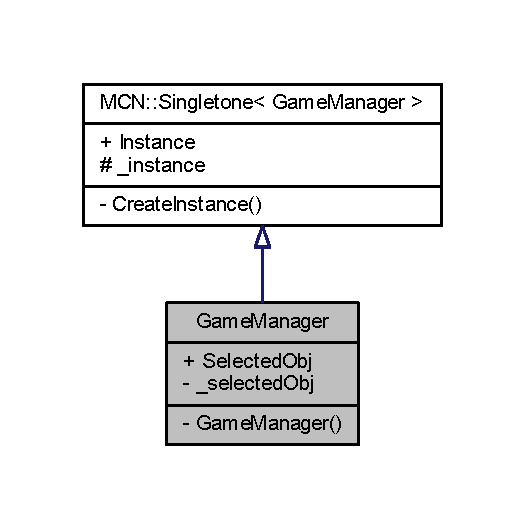
\includegraphics[width=252pt]{class_game_manager__inherit__graph}
\end{center}
\end{figure}


Game\+Manager에 대한 협력 다이어그램\+:\nopagebreak
\begin{figure}[H]
\begin{center}
\leavevmode
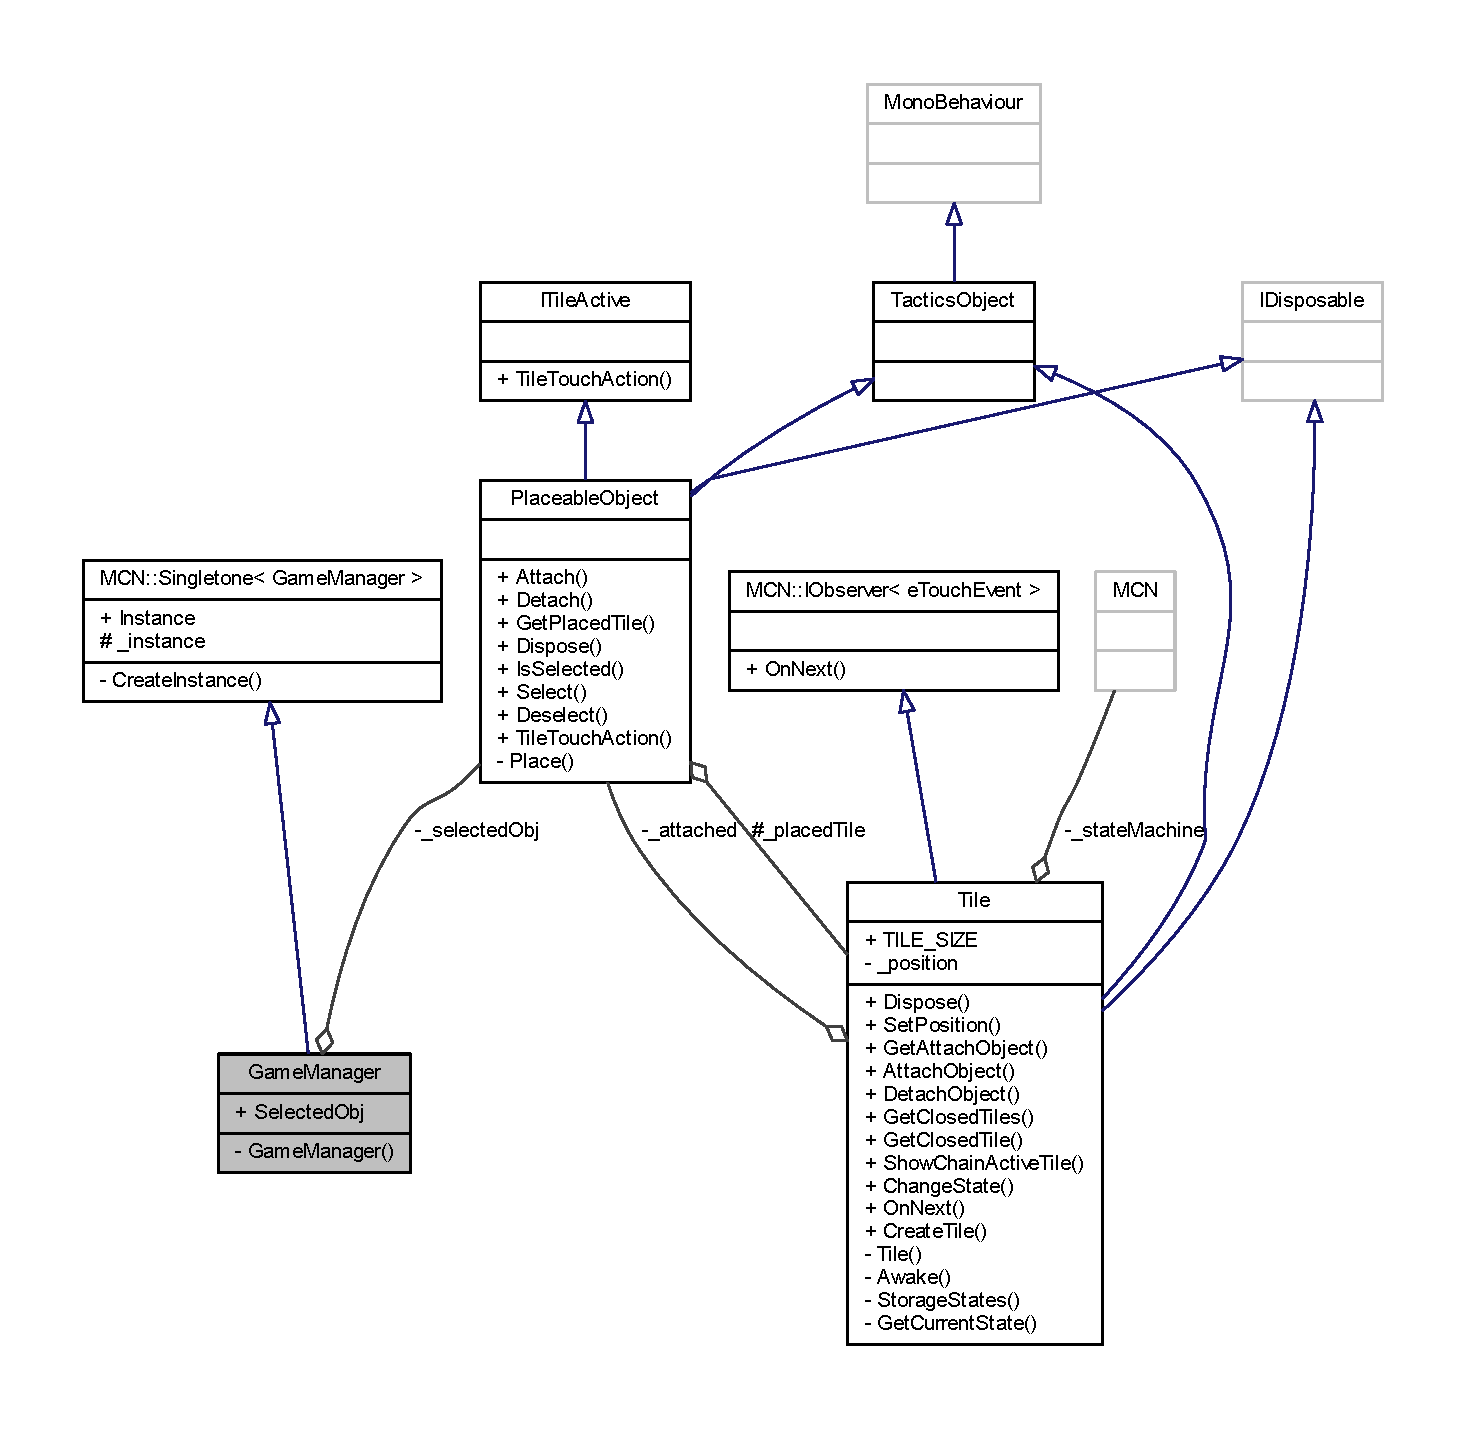
\includegraphics[width=350pt]{class_game_manager__coll__graph}
\end{center}
\end{figure}
\subsection*{정적 Protected 속성}
\begin{DoxyCompactItemize}
\item 
static T \hyperlink{class_m_c_n_1_1_singletone_a267e8a9e6e7c073b988cda4f95e26eb1}{\+\_\+instance}
\end{DoxyCompactItemize}
\subsection*{속성}
\begin{DoxyCompactItemize}
\item 
\hyperlink{class_tactics_object}{Tactics\+Object} \hyperlink{class_game_manager_a708d9fb61ea9f34e4c3a55d34c31acf2}{Selected\+Obj}\hspace{0.3cm}{\ttfamily  \mbox{[}get, set\mbox{]}}
\item 
static T \hyperlink{class_m_c_n_1_1_singletone_a46dbbebd93e96a9592a9803c51f35602}{Instance}\hspace{0.3cm}{\ttfamily  \mbox{[}get\mbox{]}}
\end{DoxyCompactItemize}
\subsection*{Private 멤버 함수}
\begin{DoxyCompactItemize}
\item 
\hyperlink{class_game_manager_aba36fa5d78b798e6707bd23c5ee55f19}{Game\+Manager} ()
\end{DoxyCompactItemize}
\subsection*{Private 속성}
\begin{DoxyCompactItemize}
\item 
\hyperlink{class_tactics_object}{Tactics\+Object} \hyperlink{class_game_manager_a5a9b1c2a22af163ddb89c8a55d2f1603}{\+\_\+selected\+Obj}
\end{DoxyCompactItemize}


\subsection{상세한 설명}


Game\+Manager.\+cs 파일의 4 번째 라인에서 정의되었습니다.



\subsection{생성자 \& 소멸자 문서화}
\index{Game\+Manager@{Game\+Manager}!Game\+Manager@{Game\+Manager}}
\index{Game\+Manager@{Game\+Manager}!Game\+Manager@{Game\+Manager}}
\subsubsection[{\texorpdfstring{Game\+Manager()}{GameManager()}}]{\setlength{\rightskip}{0pt plus 5cm}Game\+Manager.\+Game\+Manager (
\begin{DoxyParamCaption}
{}
\end{DoxyParamCaption}
)\hspace{0.3cm}{\ttfamily [private]}}\hypertarget{class_game_manager_aba36fa5d78b798e6707bd23c5ee55f19}{}\label{class_game_manager_aba36fa5d78b798e6707bd23c5ee55f19}


Game\+Manager.\+cs 파일의 21 번째 라인에서 정의되었습니다.


\begin{DoxyCode}
21 \{\}
\end{DoxyCode}


\subsection{멤버 데이타 문서화}
\index{Game\+Manager@{Game\+Manager}!\+\_\+instance@{\+\_\+instance}}
\index{\+\_\+instance@{\+\_\+instance}!Game\+Manager@{Game\+Manager}}
\subsubsection[{\texorpdfstring{\+\_\+instance}{_instance}}]{\setlength{\rightskip}{0pt plus 5cm}T {\bf M\+C\+N.\+Singletone}$<$ T $>$.\+\_\+instance\hspace{0.3cm}{\ttfamily [static]}, {\ttfamily [protected]}, {\ttfamily [inherited]}}\hypertarget{class_m_c_n_1_1_singletone_a267e8a9e6e7c073b988cda4f95e26eb1}{}\label{class_m_c_n_1_1_singletone_a267e8a9e6e7c073b988cda4f95e26eb1}


Singletone.\+cs 파일의 15 번째 라인에서 정의되었습니다.

\index{Game\+Manager@{Game\+Manager}!\+\_\+selected\+Obj@{\+\_\+selected\+Obj}}
\index{\+\_\+selected\+Obj@{\+\_\+selected\+Obj}!Game\+Manager@{Game\+Manager}}
\subsubsection[{\texorpdfstring{\+\_\+selected\+Obj}{_selectedObj}}]{\setlength{\rightskip}{0pt plus 5cm}{\bf Tactics\+Object} Game\+Manager.\+\_\+selected\+Obj\hspace{0.3cm}{\ttfamily [private]}}\hypertarget{class_game_manager_a5a9b1c2a22af163ddb89c8a55d2f1603}{}\label{class_game_manager_a5a9b1c2a22af163ddb89c8a55d2f1603}


Game\+Manager.\+cs 파일의 6 번째 라인에서 정의되었습니다.



\subsection{속성 문서화}
\index{Game\+Manager@{Game\+Manager}!Instance@{Instance}}
\index{Instance@{Instance}!Game\+Manager@{Game\+Manager}}
\subsubsection[{\texorpdfstring{Instance}{Instance}}]{\setlength{\rightskip}{0pt plus 5cm}T {\bf M\+C\+N.\+Singletone}$<$ T $>$.Instance\hspace{0.3cm}{\ttfamily [static]}, {\ttfamily [get]}, {\ttfamily [inherited]}}\hypertarget{class_m_c_n_1_1_singletone_a46dbbebd93e96a9592a9803c51f35602}{}\label{class_m_c_n_1_1_singletone_a46dbbebd93e96a9592a9803c51f35602}


Singletone.\+cs 파일의 18 번째 라인에서 정의되었습니다.

\index{Game\+Manager@{Game\+Manager}!Selected\+Obj@{Selected\+Obj}}
\index{Selected\+Obj@{Selected\+Obj}!Game\+Manager@{Game\+Manager}}
\subsubsection[{\texorpdfstring{Selected\+Obj}{SelectedObj}}]{\setlength{\rightskip}{0pt plus 5cm}{\bf Tactics\+Object} Game\+Manager.\+Selected\+Obj\hspace{0.3cm}{\ttfamily [get]}, {\ttfamily [set]}}\hypertarget{class_game_manager_a708d9fb61ea9f34e4c3a55d34c31acf2}{}\label{class_game_manager_a708d9fb61ea9f34e4c3a55d34c31acf2}


Game\+Manager.\+cs 파일의 9 번째 라인에서 정의되었습니다.



이 클래스에 대한 문서화 페이지는 다음의 파일로부터 생성되었습니다.\+:\begin{DoxyCompactItemize}
\item 
D\+:/\+Git\+Hub/\+M\+C\+N\+Tactics/\+Assets/\+Scripts/\+Manager/\hyperlink{_game_manager_8cs}{Game\+Manager.\+cs}\end{DoxyCompactItemize}

\hypertarget{interface_m_c_n_1_1_i_observable}{}\section{M\+C\+N.\+I\+Observable$<$ T $>$ 인터페이스 템플릿 참조}
\label{interface_m_c_n_1_1_i_observable}\index{M\+C\+N.\+I\+Observable$<$ T $>$@{M\+C\+N.\+I\+Observable$<$ T $>$}}


옵저버 관리자 인터페이스  




M\+C\+N.\+I\+Observable$<$ T $>$에 대한 협력 다이어그램\+:\nopagebreak
\begin{figure}[H]
\begin{center}
\leavevmode
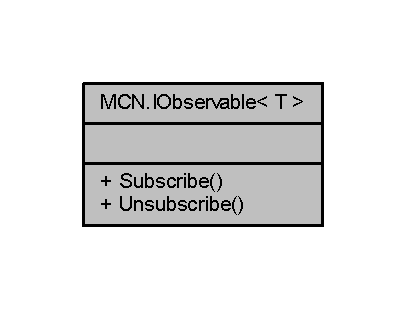
\includegraphics[width=195pt]{interface_m_c_n_1_1_i_observable__coll__graph}
\end{center}
\end{figure}
\subsection*{Public 멤버 함수}
\begin{DoxyCompactItemize}
\item 
void \hyperlink{interface_m_c_n_1_1_i_observable_a84e57296a612a2d49afbcc7f841ceb0b}{Subscribe} (\hyperlink{interface_m_c_n_1_1_i_observer}{I\+Observer}$<$ T $>$ observer)
\begin{DoxyCompactList}\small\item\em 옵저버 등록 메소드 \end{DoxyCompactList}\item 
void \hyperlink{interface_m_c_n_1_1_i_observable_a3ff752d344f0b610b1146af7a0fbf067}{Unsubscribe} (\hyperlink{interface_m_c_n_1_1_i_observer}{I\+Observer}$<$ T $>$ observer)
\begin{DoxyCompactList}\small\item\em 옵저버 등록 해제 메소드 \end{DoxyCompactList}\end{DoxyCompactItemize}


\subsection{상세한 설명}
옵저버 관리자 인터페이스 

옵저버 패턴에서 관찰자들을 관리하는 관리자 인터페이스. \begin{DoxyAuthor}{작성자}
Delight 
\end{DoxyAuthor}


I\+Observable.\+cs 파일의 10 번째 라인에서 정의되었습니다.



\subsection{멤버 함수 문서화}
\index{M\+C\+N\+::\+I\+Observable@{M\+C\+N\+::\+I\+Observable}!Subscribe@{Subscribe}}
\index{Subscribe@{Subscribe}!M\+C\+N\+::\+I\+Observable@{M\+C\+N\+::\+I\+Observable}}
\subsubsection[{\texorpdfstring{Subscribe(\+I\+Observer$<$ T $>$ observer)}{Subscribe(IObserver< T > observer)}}]{\setlength{\rightskip}{0pt plus 5cm}void {\bf M\+C\+N.\+I\+Observable}$<$ T $>$.Subscribe (
\begin{DoxyParamCaption}
\item[{{\bf I\+Observer}$<$ T $>$}]{observer}
\end{DoxyParamCaption}
)}\hypertarget{interface_m_c_n_1_1_i_observable_a84e57296a612a2d49afbcc7f841ceb0b}{}\label{interface_m_c_n_1_1_i_observable_a84e57296a612a2d49afbcc7f841ceb0b}


옵저버 등록 메소드 

구현시에는 리스트 등을 활용하여 observer를 등록해둔다. \index{M\+C\+N\+::\+I\+Observable@{M\+C\+N\+::\+I\+Observable}!Unsubscribe@{Unsubscribe}}
\index{Unsubscribe@{Unsubscribe}!M\+C\+N\+::\+I\+Observable@{M\+C\+N\+::\+I\+Observable}}
\subsubsection[{\texorpdfstring{Unsubscribe(\+I\+Observer$<$ T $>$ observer)}{Unsubscribe(IObserver< T > observer)}}]{\setlength{\rightskip}{0pt plus 5cm}void {\bf M\+C\+N.\+I\+Observable}$<$ T $>$.Unsubscribe (
\begin{DoxyParamCaption}
\item[{{\bf I\+Observer}$<$ T $>$}]{observer}
\end{DoxyParamCaption}
)}\hypertarget{interface_m_c_n_1_1_i_observable_a3ff752d344f0b610b1146af7a0fbf067}{}\label{interface_m_c_n_1_1_i_observable_a3ff752d344f0b610b1146af7a0fbf067}


옵저버 등록 해제 메소드 

등록된 리스트 등에서 해당 observer를 해제한다. 

이 인터페이스에 대한 문서화 페이지는 다음의 파일로부터 생성되었습니다.\+:\begin{DoxyCompactItemize}
\item 
D\+:/\+Git\+Hub/\+M\+C\+N\+Tactics/\+Assets/\+Scripts/\+Core/\hyperlink{_i_observable_8cs}{I\+Observable.\+cs}\end{DoxyCompactItemize}

\hypertarget{interface_m_c_n_1_1_i_observer}{}\section{M\+C\+N.\+I\+Observer$<$ T $>$ 인터페이스 템플릿 참조}
\label{interface_m_c_n_1_1_i_observer}\index{M\+C\+N.\+I\+Observer$<$ T $>$@{M\+C\+N.\+I\+Observer$<$ T $>$}}


M\+C\+N.\+I\+Observer$<$ T $>$에 대한 협력 다이어그램\+:\nopagebreak
\begin{figure}[H]
\begin{center}
\leavevmode
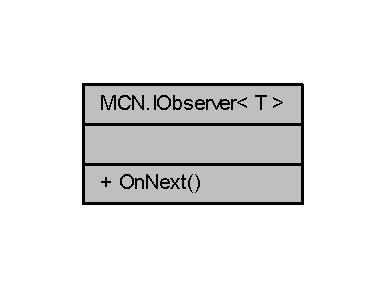
\includegraphics[width=185pt]{interface_m_c_n_1_1_i_observer__coll__graph}
\end{center}
\end{figure}
\subsection*{Public 멤버 함수}
\begin{DoxyCompactItemize}
\item 
void \hyperlink{interface_m_c_n_1_1_i_observer_a2f934b71aa4ddf6f936670d32c3cdff7}{On\+Next} (T data)
\end{DoxyCompactItemize}


\subsection{상세한 설명}


I\+Observable.\+cs 파일의 11 번째 라인에서 정의되었습니다.



\subsection{멤버 함수 문서화}
\index{M\+C\+N\+::\+I\+Observer@{M\+C\+N\+::\+I\+Observer}!On\+Next@{On\+Next}}
\index{On\+Next@{On\+Next}!M\+C\+N\+::\+I\+Observer@{M\+C\+N\+::\+I\+Observer}}
\subsubsection[{\texorpdfstring{On\+Next(\+T data)}{OnNext(T data)}}]{\setlength{\rightskip}{0pt plus 5cm}void {\bf M\+C\+N.\+I\+Observer}$<$ T $>$.On\+Next (
\begin{DoxyParamCaption}
\item[{T}]{data}
\end{DoxyParamCaption}
)}\hypertarget{interface_m_c_n_1_1_i_observer_a2f934b71aa4ddf6f936670d32c3cdff7}{}\label{interface_m_c_n_1_1_i_observer_a2f934b71aa4ddf6f936670d32c3cdff7}


이 인터페이스에 대한 문서화 페이지는 다음의 파일로부터 생성되었습니다.\+:\begin{DoxyCompactItemize}
\item 
D\+:/\+Git\+Hub/\+M\+C\+N\+Tactics/\+Assets/\+Scripts/\+Core/\hyperlink{_i_observable_8cs}{I\+Observable.\+cs}\end{DoxyCompactItemize}

\hypertarget{class_map_creator}{}\section{Map\+Creator 클래스 참조}
\label{class_map_creator}\index{Map\+Creator@{Map\+Creator}}


Map\+Creator에 대한 협력 다이어그램\+:\nopagebreak
\begin{figure}[H]
\begin{center}
\leavevmode
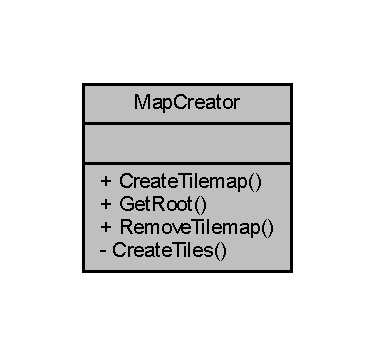
\includegraphics[width=180pt]{class_map_creator__coll__graph}
\end{center}
\end{figure}
\subsection*{Public 멤버 함수}
\begin{DoxyCompactItemize}
\item 
void \hyperlink{class_map_creator_a80d7f9ebca92a02da259157958929a6d}{Create\+Tilemap} (Vector2 map\+Size, ref Dictionary$<$ Vector2, \hyperlink{class_tile}{Tile} $>$ result\+Tilemap)
\item 
Game\+Object \hyperlink{class_map_creator_aa7308965858123141f44438bb017acc8}{Get\+Root} ()
\item 
void \hyperlink{class_map_creator_afb12afa9a9ca8fe04701af4b494e1c8a}{Remove\+Tilemap} (ref Dictionary$<$ Vector2, \hyperlink{class_tile}{Tile} $>$ tilemap)
\end{DoxyCompactItemize}
\subsection*{Private 멤버 함수}
\begin{DoxyCompactItemize}
\item 
void \hyperlink{class_map_creator_aff7c3fbefa2dd4f091ded379ca000a23}{Create\+Tiles} (Vector2 map\+Size, ref Dictionary$<$ Vector2, \hyperlink{class_tile}{Tile} $>$ tilemap)
\end{DoxyCompactItemize}


\subsection{상세한 설명}


Map\+Creator.\+cs 파일의 6 번째 라인에서 정의되었습니다.



\subsection{멤버 함수 문서화}
\index{Map\+Creator@{Map\+Creator}!Create\+Tilemap@{Create\+Tilemap}}
\index{Create\+Tilemap@{Create\+Tilemap}!Map\+Creator@{Map\+Creator}}
\subsubsection[{\texorpdfstring{Create\+Tilemap(\+Vector2 map\+Size, ref Dictionary$<$ Vector2, Tile $>$ result\+Tilemap)}{CreateTilemap(Vector2 mapSize, ref Dictionary< Vector2, Tile > resultTilemap)}}]{\setlength{\rightskip}{0pt plus 5cm}void Map\+Creator.\+Create\+Tilemap (
\begin{DoxyParamCaption}
\item[{Vector2}]{map\+Size, }
\item[{ref Dictionary$<$ Vector2, {\bf Tile} $>$}]{result\+Tilemap}
\end{DoxyParamCaption}
)}\hypertarget{class_map_creator_a80d7f9ebca92a02da259157958929a6d}{}\label{class_map_creator_a80d7f9ebca92a02da259157958929a6d}


Map\+Creator.\+cs 파일의 8 번째 라인에서 정의되었습니다.


\begin{DoxyCode}
9     \{
10         \hyperlink{class_map_creator_afb12afa9a9ca8fe04701af4b494e1c8a}{RemoveTilemap}(ref resultTilemap);
11 
12         \hyperlink{class_map_creator_aff7c3fbefa2dd4f091ded379ca000a23}{CreateTiles}(mapSize, ref resultTilemap);
13     \}
\end{DoxyCode}


이 함수 내부에서 호출하는 함수들에 대한 그래프입니다.\+:
% FIG 0




이 함수를 호출하는 함수들에 대한 그래프입니다.\+:\nopagebreak
\begin{figure}[H]
\begin{center}
\leavevmode
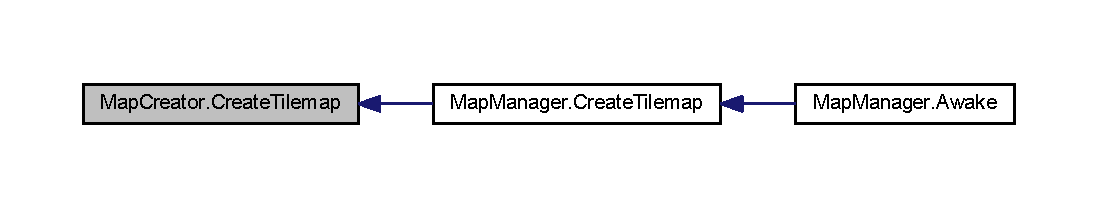
\includegraphics[width=350pt]{class_map_creator_a80d7f9ebca92a02da259157958929a6d_icgraph}
\end{center}
\end{figure}


\index{Map\+Creator@{Map\+Creator}!Create\+Tiles@{Create\+Tiles}}
\index{Create\+Tiles@{Create\+Tiles}!Map\+Creator@{Map\+Creator}}
\subsubsection[{\texorpdfstring{Create\+Tiles(\+Vector2 map\+Size, ref Dictionary$<$ Vector2, Tile $>$ tilemap)}{CreateTiles(Vector2 mapSize, ref Dictionary< Vector2, Tile > tilemap)}}]{\setlength{\rightskip}{0pt plus 5cm}void Map\+Creator.\+Create\+Tiles (
\begin{DoxyParamCaption}
\item[{Vector2}]{map\+Size, }
\item[{ref Dictionary$<$ Vector2, {\bf Tile} $>$}]{tilemap}
\end{DoxyParamCaption}
)\hspace{0.3cm}{\ttfamily [private]}}\hypertarget{class_map_creator_aff7c3fbefa2dd4f091ded379ca000a23}{}\label{class_map_creator_aff7c3fbefa2dd4f091ded379ca000a23}


Map\+Creator.\+cs 파일의 48 번째 라인에서 정의되었습니다.


\begin{DoxyCode}
49     \{
50         \textcolor{keywordflow}{if} (mapSize.x <= 0 && mapSize.y <= 0)
51         \{
52             \textcolor{keywordflow}{return};
53         \}
54 
55         \textcolor{keywordflow}{if} (tilemap == null)
56         \{
57             tilemap = \textcolor{keyword}{new} Dictionary<Vector2, Tile>();
58         \}
59 
60         var offset = 0.03f;
61 
62         \textcolor{keywordflow}{for} (\textcolor{keywordtype}{int} i = 0; i < mapSize.x; ++i)
63         \{
64             \textcolor{keywordflow}{for} (\textcolor{keywordtype}{int} j = 0; j < mapSize.y; ++j)
65             \{
66                 var tilePosition = \textcolor{keyword}{new} Vector2(i, j);
67 
68                 var tile = \hyperlink{class_tile}{Tile}.\hyperlink{class_tile_aec3cdb55a67f4c12d3056355c15bdba2}{CreateTile}(tilePosition);
69 
70                 tile.transform.position = \textcolor{keyword}{new} Vector3(i * (\hyperlink{class_tile}{Tile}.\hyperlink{class_tile_a51b7dea4344573ba12a461a32517e683}{TILE\_SIZE} + offset), 0, j * (
      \hyperlink{class_tile}{Tile}.\hyperlink{class_tile_a51b7dea4344573ba12a461a32517e683}{TILE\_SIZE} + offset));
71 
72                 tile.transform.parent = \hyperlink{class_map_creator_aa7308965858123141f44438bb017acc8}{GetRoot}().transform;
73 
74                 tilemap[tilePosition] = tile.GetComponent<\hyperlink{class_tile}{Tile}>();
75                 tilemap[tilePosition].\hyperlink{class_tile_a4d7a81b36513066aad741ed675164690}{SetPosition}(tilePosition);
76             \}
77         \}
78     \}
\end{DoxyCode}


이 함수 내부에서 호출하는 함수들에 대한 그래프입니다.\+:\nopagebreak
\begin{figure}[H]
\begin{center}
\leavevmode
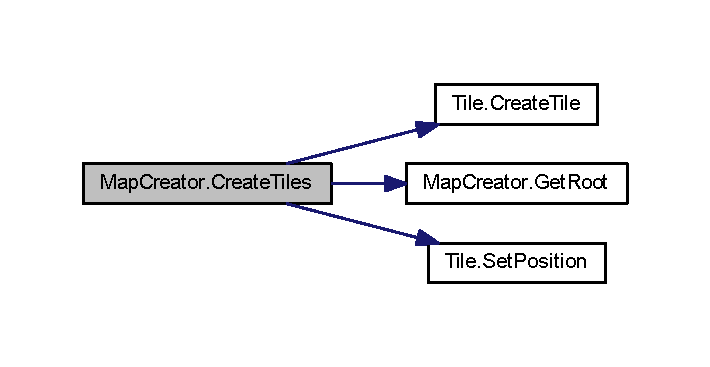
\includegraphics[width=341pt]{class_map_creator_aff7c3fbefa2dd4f091ded379ca000a23_cgraph}
\end{center}
\end{figure}




이 함수를 호출하는 함수들에 대한 그래프입니다.\+:\nopagebreak
\begin{figure}[H]
\begin{center}
\leavevmode
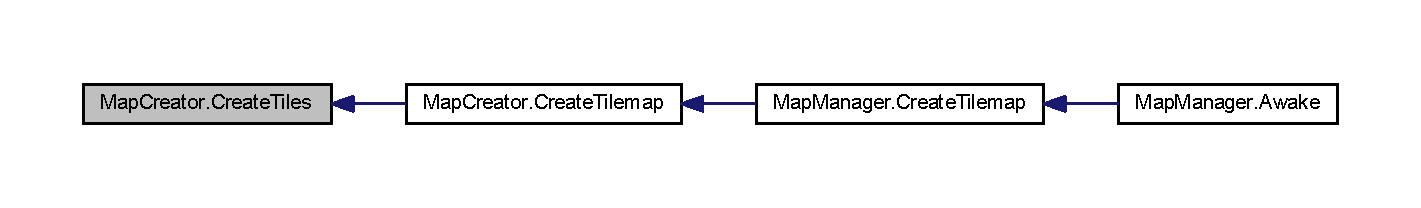
\includegraphics[width=350pt]{class_map_creator_aff7c3fbefa2dd4f091ded379ca000a23_icgraph}
\end{center}
\end{figure}


\index{Map\+Creator@{Map\+Creator}!Get\+Root@{Get\+Root}}
\index{Get\+Root@{Get\+Root}!Map\+Creator@{Map\+Creator}}
\subsubsection[{\texorpdfstring{Get\+Root()}{GetRoot()}}]{\setlength{\rightskip}{0pt plus 5cm}Game\+Object Map\+Creator.\+Get\+Root (
\begin{DoxyParamCaption}
{}
\end{DoxyParamCaption}
)}\hypertarget{class_map_creator_aa7308965858123141f44438bb017acc8}{}\label{class_map_creator_aa7308965858123141f44438bb017acc8}


Map\+Creator.\+cs 파일의 15 번째 라인에서 정의되었습니다.


\begin{DoxyCode}
16     \{
17         var root = GameObject.Find(\textcolor{stringliteral}{"Tilemap"});
18 
19         \textcolor{keywordflow}{if} (root == null)
20         \{
21             root = \textcolor{keyword}{new} GameObject(\textcolor{stringliteral}{"Tilemap"});
22             root.transform.position = Vector3.up * -1;
23         \}
24 
25         \textcolor{keywordflow}{return} root;
26     \}
\end{DoxyCode}


이 함수를 호출하는 함수들에 대한 그래프입니다.\+:\nopagebreak
\begin{figure}[H]
\begin{center}
\leavevmode
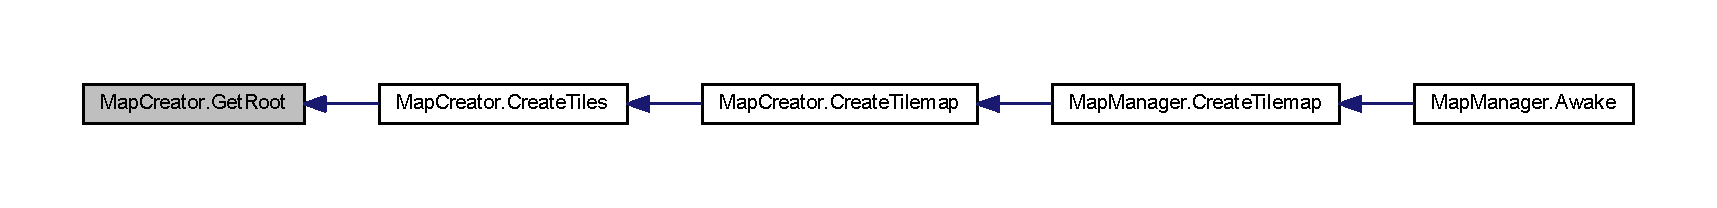
\includegraphics[width=350pt]{class_map_creator_aa7308965858123141f44438bb017acc8_icgraph}
\end{center}
\end{figure}


\index{Map\+Creator@{Map\+Creator}!Remove\+Tilemap@{Remove\+Tilemap}}
\index{Remove\+Tilemap@{Remove\+Tilemap}!Map\+Creator@{Map\+Creator}}
\subsubsection[{\texorpdfstring{Remove\+Tilemap(ref Dictionary$<$ Vector2, Tile $>$ tilemap)}{RemoveTilemap(ref Dictionary< Vector2, Tile > tilemap)}}]{\setlength{\rightskip}{0pt plus 5cm}void Map\+Creator.\+Remove\+Tilemap (
\begin{DoxyParamCaption}
\item[{ref Dictionary$<$ Vector2, {\bf Tile} $>$}]{tilemap}
\end{DoxyParamCaption}
)}\hypertarget{class_map_creator_afb12afa9a9ca8fe04701af4b494e1c8a}{}\label{class_map_creator_afb12afa9a9ca8fe04701af4b494e1c8a}


Map\+Creator.\+cs 파일의 28 번째 라인에서 정의되었습니다.


\begin{DoxyCode}
29     \{
30         \textcolor{keywordflow}{if}(tilemap == null)
31         \{
32             \textcolor{keywordflow}{return};
33         \}
34 
35         \textcolor{keywordflow}{foreach} (var tilePair \textcolor{keywordflow}{in} tilemap)
36         \{
37             var tile = tilePair.Value.GetComponent<\hyperlink{class_tile}{Tile}>();
38 
39             \textcolor{keywordflow}{if} (tile != null)
40             \{
41                 tile.\hyperlink{class_tile_a6e8a801e95a29156cbf32024e45c6596}{Dispose}();
42             \}
43         \}
44 
45         tilemap.Clear();
46     \}
\end{DoxyCode}


이 함수 내부에서 호출하는 함수들에 대한 그래프입니다.\+:
% FIG 1




이 함수를 호출하는 함수들에 대한 그래프입니다.\+:\nopagebreak
\begin{figure}[H]
\begin{center}
\leavevmode
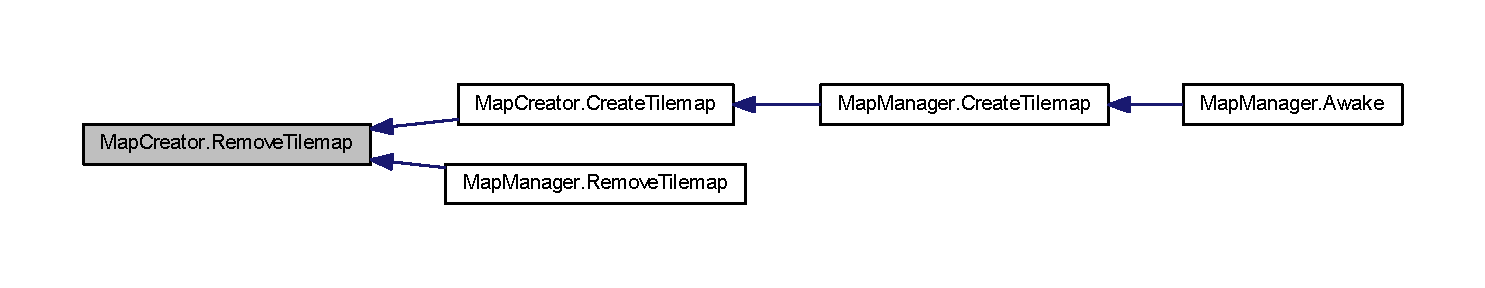
\includegraphics[width=350pt]{class_map_creator_afb12afa9a9ca8fe04701af4b494e1c8a_icgraph}
\end{center}
\end{figure}




이 클래스에 대한 문서화 페이지는 다음의 파일로부터 생성되었습니다.\+:\begin{DoxyCompactItemize}
\item 
D\+:/\+Git\+Hub/\+M\+C\+N\+Tactics/\+Assets/\+Scripts/\+Manager/\hyperlink{_map_creator_8cs}{Map\+Creator.\+cs}\end{DoxyCompactItemize}

\hypertarget{class_map_manager}{}\section{Map\+Manager 클래스 참조}
\label{class_map_manager}\index{Map\+Manager@{Map\+Manager}}


Map\+Manager에 대한 상속 다이어그램 \+: \nopagebreak
\begin{figure}[H]
\begin{center}
\leavevmode
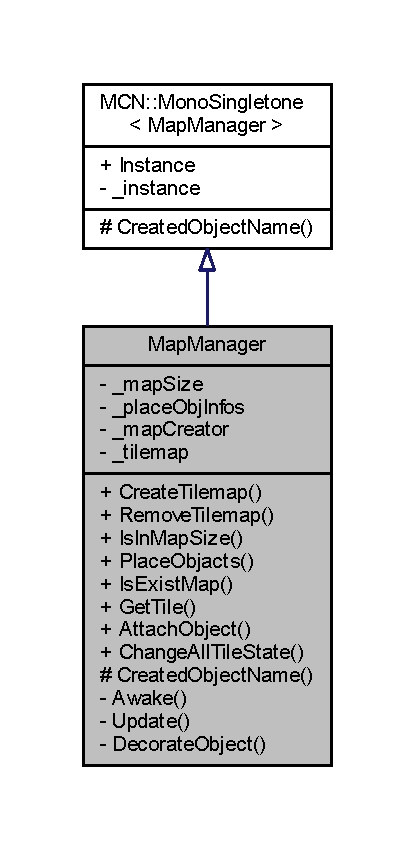
\includegraphics[width=199pt]{class_map_manager__inherit__graph}
\end{center}
\end{figure}


Map\+Manager에 대한 협력 다이어그램\+:\nopagebreak
\begin{figure}[H]
\begin{center}
\leavevmode
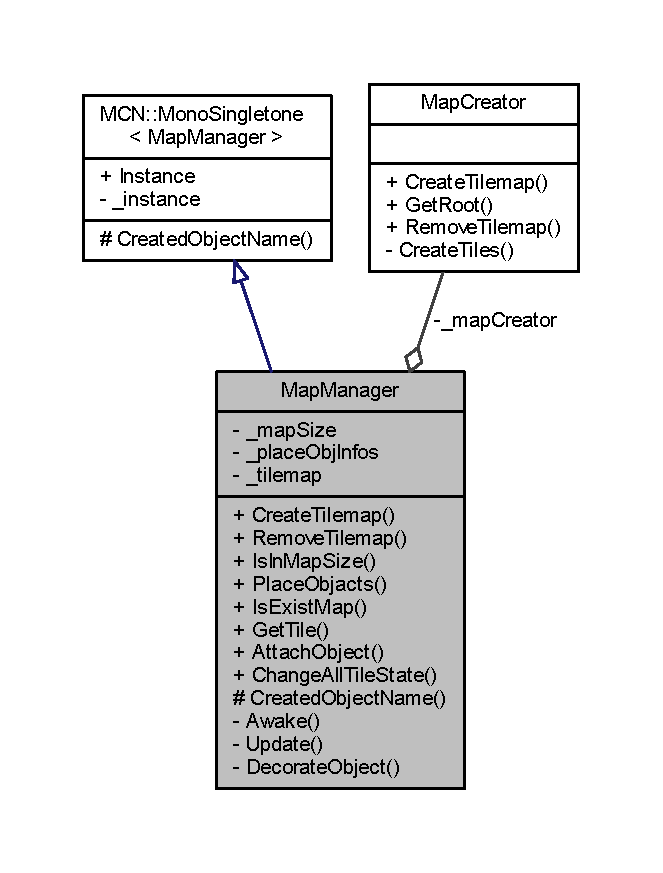
\includegraphics[width=318pt]{class_map_manager__coll__graph}
\end{center}
\end{figure}
\subsection*{클래스}
\begin{DoxyCompactItemize}
\item 
class \hyperlink{class_map_manager_1_1_place_info}{Place\+Info}
\end{DoxyCompactItemize}
\subsection*{Public 멤버 함수}
\begin{DoxyCompactItemize}
\item 
void \hyperlink{class_map_manager_aa6125f2ca4b3c4e8858f73f5e65d385b}{Create\+Tilemap} ()
\item 
void \hyperlink{class_map_manager_aac20afabde4946e32ce1e719c72e0f50}{Remove\+Tilemap} ()
\item 
bool \hyperlink{class_map_manager_a504d7a68ace64557bc3c3254a8b1cddc}{Is\+In\+Map\+Size} (Vector2 pos)
\item 
void \hyperlink{class_map_manager_a4213ccbaa1a81d0a47884de50a28de32}{Place\+Objacts} ()
\item 
bool \hyperlink{class_map_manager_a9a18efae73b0d690d2bc6c8ac8703a02}{Is\+Exist\+Map} ()
\item 
\hyperlink{class_tile}{Tile} \hyperlink{class_map_manager_ae457099efdd1a804add3b851b2bc7691}{Get\+Tile} (Vector2 position)
\item 
void \hyperlink{class_map_manager_ab8cbf46e369a9c59ff183a1b6c3b20bb}{Attach\+Object} (Vector2 pos, \hyperlink{class_placeable_object}{Placeable\+Object} obj)
\item 
void \hyperlink{class_map_manager_a68f796431393b7239320ab1f5200213a}{Change\+All\+Tile\+State} (\hyperlink{_tile_8cs_a271bc07be325bca511bcb747e0ff2fda}{e\+Tile\+Type} state)
\end{DoxyCompactItemize}
\subsection*{Protected 멤버 함수}
\begin{DoxyCompactItemize}
\item 
override string \hyperlink{class_map_manager_aa3459a9fe2d748c6e9f2c3da8a6273cd}{Created\+Object\+Name} ()
\end{DoxyCompactItemize}
\subsection*{속성}
\begin{DoxyCompactItemize}
\item 
static T \hyperlink{class_m_c_n_1_1_mono_singletone_aa50c027cca64cf4ad30c1ee5c83e0b78}{Instance}\hspace{0.3cm}{\ttfamily  \mbox{[}get\mbox{]}}
\end{DoxyCompactItemize}
\subsection*{Private 멤버 함수}
\begin{DoxyCompactItemize}
\item 
void \hyperlink{class_map_manager_ad633984007048c7d63eab44aaeb0c32d}{Awake} ()
\item 
void \hyperlink{class_map_manager_aeaf61c0a498d98a5ac778db479353d77}{Update} ()
\end{DoxyCompactItemize}
\subsection*{Private 속성}
\begin{DoxyCompactItemize}
\item 
Vector2 \hyperlink{class_map_manager_a960f398cc92f569f620ddc8c0140a5c7}{\+\_\+map\+Size}
\item 
List$<$ \hyperlink{class_map_manager_1_1_place_info}{Place\+Info} $>$ \hyperlink{class_map_manager_ab581d2c754246f74999a0b744ba2b14f}{\+\_\+place\+Obj\+Infos}
\item 
\hyperlink{class_map_creator}{Map\+Creator} \hyperlink{class_map_manager_aa837a852f355a33b263c1bb07c6c4ece}{\+\_\+map\+Creator}
\item 
Dictionary$<$ Vector2, \hyperlink{class_tile}{Tile} $>$ \hyperlink{class_map_manager_a58f7635d8e19795f3845a3f85e2b4ac3}{\+\_\+tilemap}
\end{DoxyCompactItemize}


\subsection{상세한 설명}


Map\+Manager.\+cs 파일의 5 번째 라인에서 정의되었습니다.



\subsection{멤버 함수 문서화}
\index{Map\+Manager@{Map\+Manager}!Attach\+Object@{Attach\+Object}}
\index{Attach\+Object@{Attach\+Object}!Map\+Manager@{Map\+Manager}}
\subsubsection[{\texorpdfstring{Attach\+Object(\+Vector2 pos, Placeable\+Object obj)}{AttachObject(Vector2 pos, PlaceableObject obj)}}]{\setlength{\rightskip}{0pt plus 5cm}void Map\+Manager.\+Attach\+Object (
\begin{DoxyParamCaption}
\item[{Vector2}]{pos, }
\item[{{\bf Placeable\+Object}}]{obj}
\end{DoxyParamCaption}
)}\hypertarget{class_map_manager_ab8cbf46e369a9c59ff183a1b6c3b20bb}{}\label{class_map_manager_ab8cbf46e369a9c59ff183a1b6c3b20bb}


Map\+Manager.\+cs 파일의 145 번째 라인에서 정의되었습니다.


\begin{DoxyCode}
146     \{
147         var tile = \hyperlink{class_map_manager_ae457099efdd1a804add3b851b2bc7691}{GetTile}(pos);
148 
149         \textcolor{keywordflow}{if} (tile != null)
150         \{
151             tile.AttachObject(obj);
152         \}
153     \}
\end{DoxyCode}


이 함수 내부에서 호출하는 함수들에 대한 그래프입니다.\+:\nopagebreak
\begin{figure}[H]
\begin{center}
\leavevmode
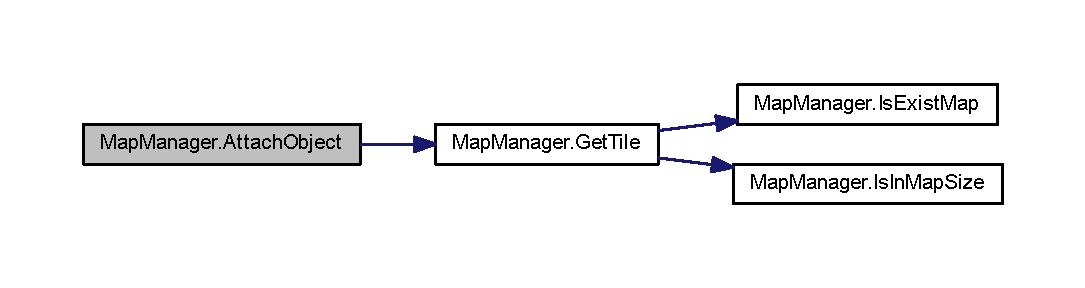
\includegraphics[width=350pt]{class_map_manager_ab8cbf46e369a9c59ff183a1b6c3b20bb_cgraph}
\end{center}
\end{figure}




이 함수를 호출하는 함수들에 대한 그래프입니다.\+:\nopagebreak
\begin{figure}[H]
\begin{center}
\leavevmode
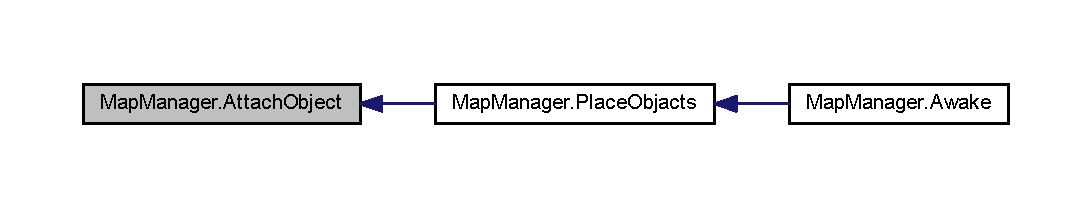
\includegraphics[width=350pt]{class_map_manager_ab8cbf46e369a9c59ff183a1b6c3b20bb_icgraph}
\end{center}
\end{figure}


\index{Map\+Manager@{Map\+Manager}!Awake@{Awake}}
\index{Awake@{Awake}!Map\+Manager@{Map\+Manager}}
\subsubsection[{\texorpdfstring{Awake()}{Awake()}}]{\setlength{\rightskip}{0pt plus 5cm}void Map\+Manager.\+Awake (
\begin{DoxyParamCaption}
{}
\end{DoxyParamCaption}
)\hspace{0.3cm}{\ttfamily [private]}}\hypertarget{class_map_manager_ad633984007048c7d63eab44aaeb0c32d}{}\label{class_map_manager_ad633984007048c7d63eab44aaeb0c32d}


Map\+Manager.\+cs 파일의 49 번째 라인에서 정의되었습니다.


\begin{DoxyCode}
50     \{
51         \textcolor{keywordflow}{if} (\hyperlink{class_map_manager_aa837a852f355a33b263c1bb07c6c4ece}{\_mapCreator} == null)
52         \{
53             \hyperlink{class_map_manager_aa837a852f355a33b263c1bb07c6c4ece}{\_mapCreator} = \textcolor{keyword}{new} \hyperlink{class_map_creator}{MapCreator}();
54         \}
55 
56         \textcolor{keywordflow}{if} (\hyperlink{class_map_manager_ab581d2c754246f74999a0b744ba2b14f}{\_placeObjInfos} == null)
57         \{
58             \hyperlink{class_map_manager_ab581d2c754246f74999a0b744ba2b14f}{\_placeObjInfos} = \textcolor{keyword}{new} List<PlaceInfo>();
59         \}
60 
61 \textcolor{preprocessor}{#if UNITY\_EDITOR}
62         \_debug = \textcolor{keyword}{new} DebugMapManager();
63         \_debug.CreateTilemap(\textcolor{keyword}{this});
64 \textcolor{preprocessor}{#else}
65         \hyperlink{class_map_manager_aa6125f2ca4b3c4e8858f73f5e65d385b}{CreateTilemap}();
66 
67         \hyperlink{class_map_manager_a4213ccbaa1a81d0a47884de50a28de32}{PlaceObjacts}();
68 \textcolor{preprocessor}{#endif}
69     \}
\end{DoxyCode}


이 함수 내부에서 호출하는 함수들에 대한 그래프입니다.\+:\nopagebreak
\begin{figure}[H]
\begin{center}
\leavevmode
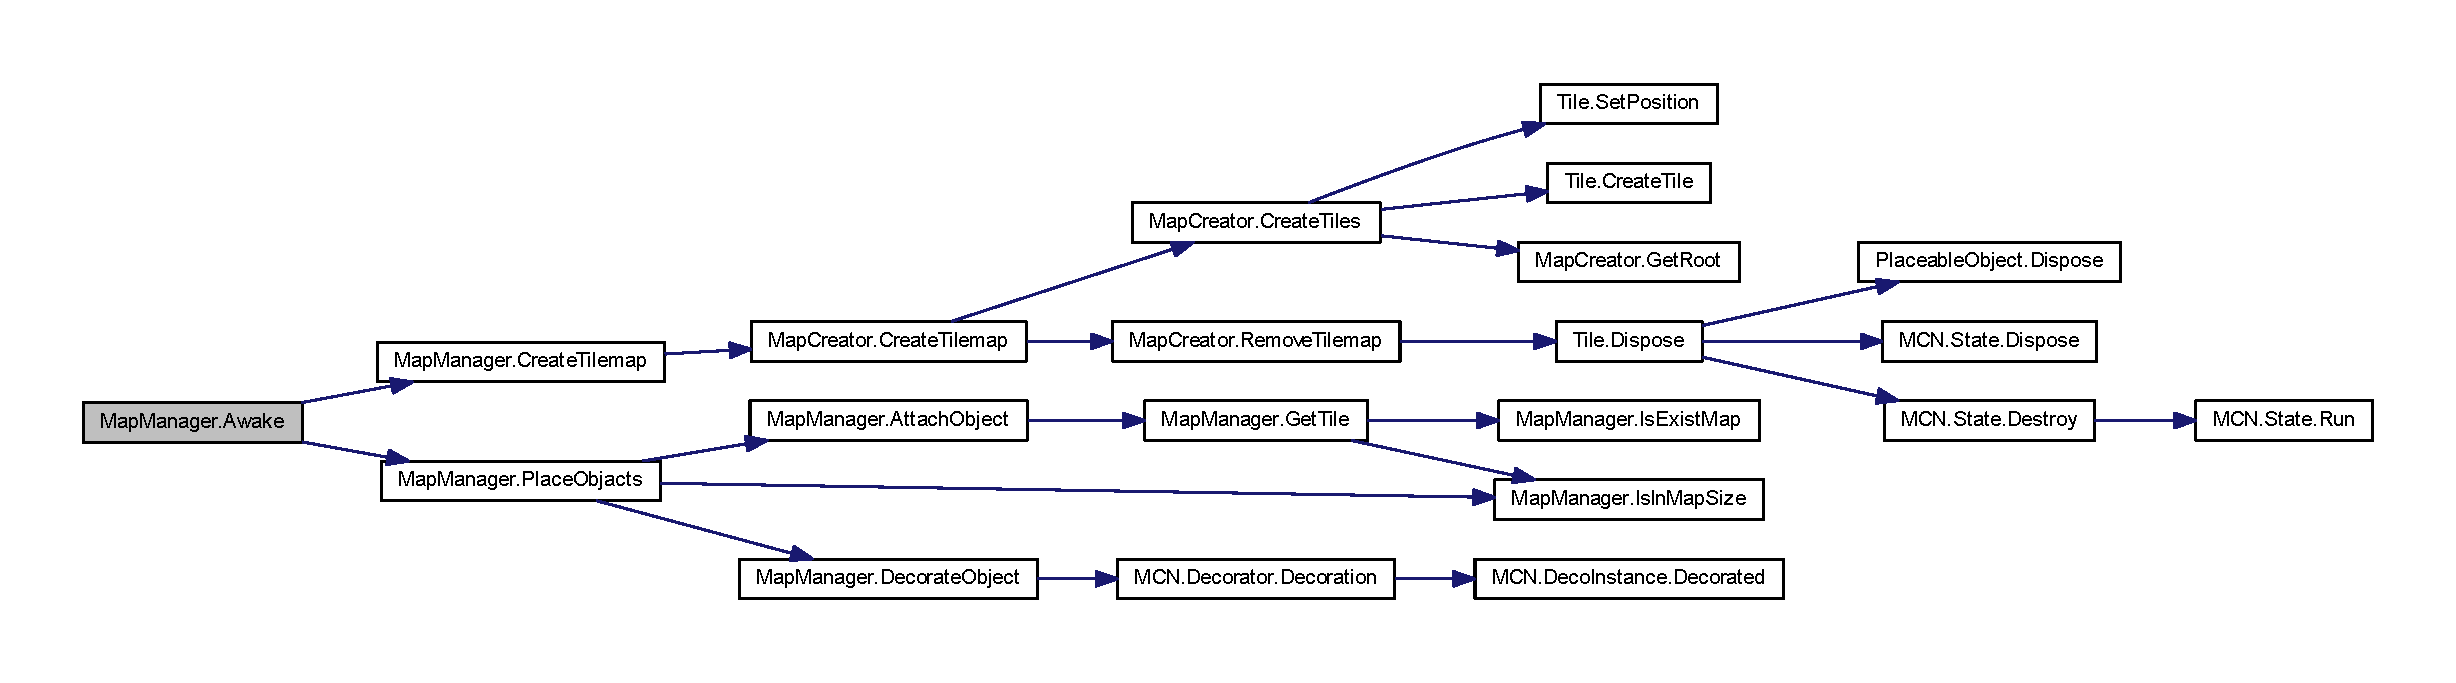
\includegraphics[width=350pt]{class_map_manager_ad633984007048c7d63eab44aaeb0c32d_cgraph}
\end{center}
\end{figure}


\index{Map\+Manager@{Map\+Manager}!Change\+All\+Tile\+State@{Change\+All\+Tile\+State}}
\index{Change\+All\+Tile\+State@{Change\+All\+Tile\+State}!Map\+Manager@{Map\+Manager}}
\subsubsection[{\texorpdfstring{Change\+All\+Tile\+State(e\+Tile\+Type state)}{ChangeAllTileState(eTileType state)}}]{\setlength{\rightskip}{0pt plus 5cm}void Map\+Manager.\+Change\+All\+Tile\+State (
\begin{DoxyParamCaption}
\item[{{\bf e\+Tile\+Type}}]{state}
\end{DoxyParamCaption}
)}\hypertarget{class_map_manager_a68f796431393b7239320ab1f5200213a}{}\label{class_map_manager_a68f796431393b7239320ab1f5200213a}


Map\+Manager.\+cs 파일의 155 번째 라인에서 정의되었습니다.


\begin{DoxyCode}
156     \{
157         \textcolor{keywordflow}{foreach}(var tile \textcolor{keywordflow}{in} \hyperlink{class_map_manager_a58f7635d8e19795f3845a3f85e2b4ac3}{\_tilemap})
158         \{
159             tile.Value.ChangeState(state);
160         \}
161     \}
\end{DoxyCode}
\index{Map\+Manager@{Map\+Manager}!Created\+Object\+Name@{Created\+Object\+Name}}
\index{Created\+Object\+Name@{Created\+Object\+Name}!Map\+Manager@{Map\+Manager}}
\subsubsection[{\texorpdfstring{Created\+Object\+Name()}{CreatedObjectName()}}]{\setlength{\rightskip}{0pt plus 5cm}override string Map\+Manager.\+Created\+Object\+Name (
\begin{DoxyParamCaption}
{}
\end{DoxyParamCaption}
)\hspace{0.3cm}{\ttfamily [protected]}, {\ttfamily [virtual]}}\hypertarget{class_map_manager_aa3459a9fe2d748c6e9f2c3da8a6273cd}{}\label{class_map_manager_aa3459a9fe2d748c6e9f2c3da8a6273cd}


\hyperlink{class_m_c_n_1_1_mono_singletone_a3dde6c2c7e6a3723102f059a043aed22}{M\+C\+N.\+Mono\+Singletone$<$ Map\+Manager $>$}를 구현.



Map\+Manager.\+cs 파일의 44 번째 라인에서 정의되었습니다.


\begin{DoxyCode}
45     \{
46         \textcolor{keywordflow}{return} \textcolor{stringliteral}{"MapManager"};
47     \}
\end{DoxyCode}
\index{Map\+Manager@{Map\+Manager}!Create\+Tilemap@{Create\+Tilemap}}
\index{Create\+Tilemap@{Create\+Tilemap}!Map\+Manager@{Map\+Manager}}
\subsubsection[{\texorpdfstring{Create\+Tilemap()}{CreateTilemap()}}]{\setlength{\rightskip}{0pt plus 5cm}void Map\+Manager.\+Create\+Tilemap (
\begin{DoxyParamCaption}
{}
\end{DoxyParamCaption}
)}\hypertarget{class_map_manager_aa6125f2ca4b3c4e8858f73f5e65d385b}{}\label{class_map_manager_aa6125f2ca4b3c4e8858f73f5e65d385b}


Map\+Manager.\+cs 파일의 78 번째 라인에서 정의되었습니다.


\begin{DoxyCode}
79     \{
80         \textcolor{keywordflow}{if} (\hyperlink{class_map_manager_aa837a852f355a33b263c1bb07c6c4ece}{\_mapCreator} != null)
81         \{
82             \hyperlink{class_map_manager_aa837a852f355a33b263c1bb07c6c4ece}{\_mapCreator}.\hyperlink{class_map_creator_a80d7f9ebca92a02da259157958929a6d}{CreateTilemap}(\hyperlink{class_map_manager_a960f398cc92f569f620ddc8c0140a5c7}{\_mapSize}, ref 
      \hyperlink{class_map_manager_a58f7635d8e19795f3845a3f85e2b4ac3}{\_tilemap});
83         \}
84     \}
\end{DoxyCode}


이 함수 내부에서 호출하는 함수들에 대한 그래프입니다.\+:\nopagebreak
\begin{figure}[H]
\begin{center}
\leavevmode
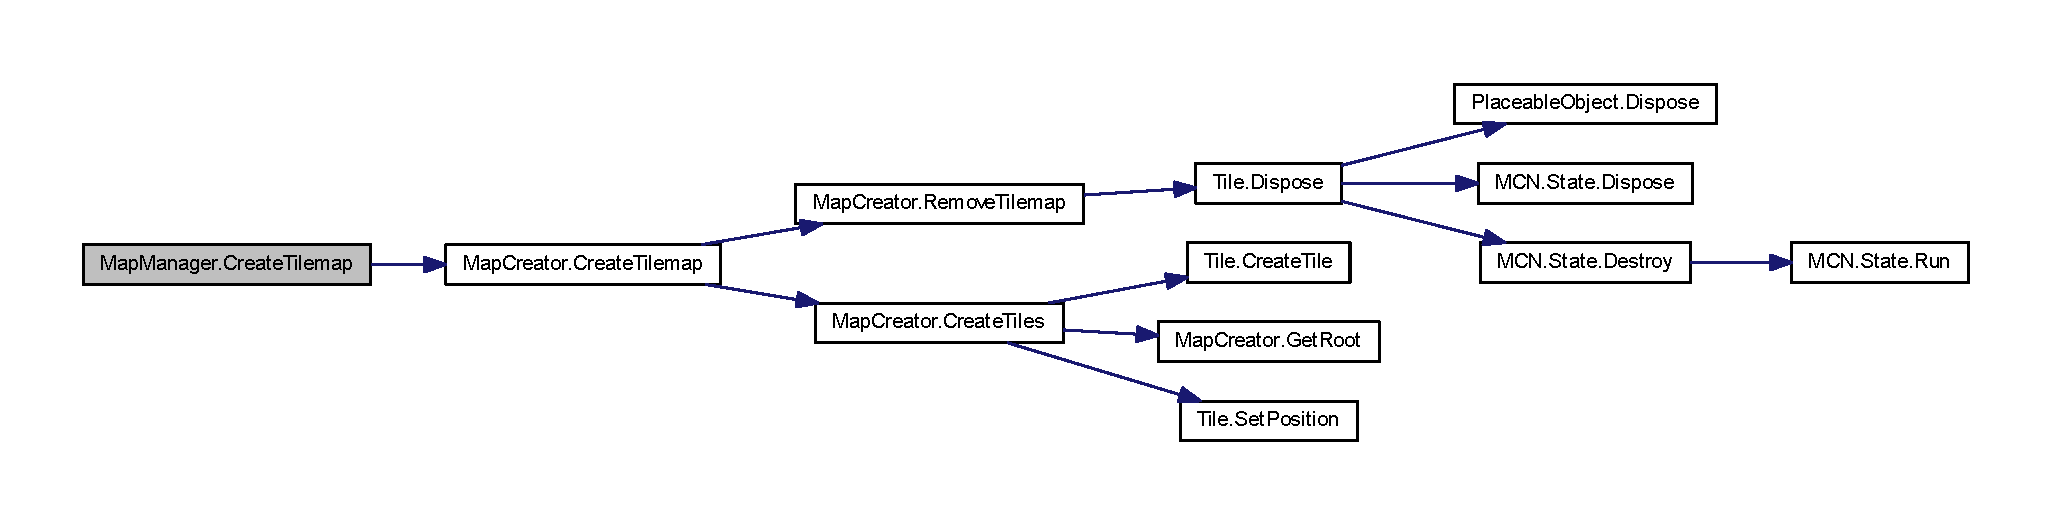
\includegraphics[width=350pt]{class_map_manager_aa6125f2ca4b3c4e8858f73f5e65d385b_cgraph}
\end{center}
\end{figure}




이 함수를 호출하는 함수들에 대한 그래프입니다.\+:\nopagebreak
\begin{figure}[H]
\begin{center}
\leavevmode
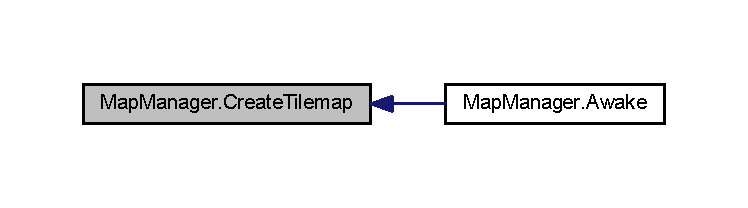
\includegraphics[width=350pt]{class_map_manager_aa6125f2ca4b3c4e8858f73f5e65d385b_icgraph}
\end{center}
\end{figure}


\index{Map\+Manager@{Map\+Manager}!Get\+Tile@{Get\+Tile}}
\index{Get\+Tile@{Get\+Tile}!Map\+Manager@{Map\+Manager}}
\subsubsection[{\texorpdfstring{Get\+Tile(\+Vector2 position)}{GetTile(Vector2 position)}}]{\setlength{\rightskip}{0pt plus 5cm}{\bf Tile} Map\+Manager.\+Get\+Tile (
\begin{DoxyParamCaption}
\item[{Vector2}]{position}
\end{DoxyParamCaption}
)}\hypertarget{class_map_manager_ae457099efdd1a804add3b851b2bc7691}{}\label{class_map_manager_ae457099efdd1a804add3b851b2bc7691}


Map\+Manager.\+cs 파일의 128 번째 라인에서 정의되었습니다.


\begin{DoxyCode}
129     \{
130         \textcolor{keywordflow}{if} (\hyperlink{class_map_manager_a9a18efae73b0d690d2bc6c8ac8703a02}{IsExistMap}())
131         \{
132             \textcolor{keywordflow}{if} (\hyperlink{class_map_manager_a504d7a68ace64557bc3c3254a8b1cddc}{IsInMapSize}(position))
133             \{
134                 \textcolor{keywordflow}{return} \hyperlink{class_map_manager_a58f7635d8e19795f3845a3f85e2b4ac3}{\_tilemap}[position];
135             \}
136 
137             \textcolor{keywordflow}{return} null;
138         \}
139         \textcolor{keywordflow}{else}
140         \{
141             \textcolor{keywordflow}{throw} \textcolor{keyword}{new} UnityException(\textcolor{stringliteral}{"Tilemap is not exist."});
142         \}
143     \}
\end{DoxyCode}


이 함수 내부에서 호출하는 함수들에 대한 그래프입니다.\+:\nopagebreak
\begin{figure}[H]
\begin{center}
\leavevmode
\includegraphics[width=350pt]{class_map_manager_ae457099efdd1a804add3b851b2bc7691_cgraph}
\end{center}
\end{figure}




이 함수를 호출하는 함수들에 대한 그래프입니다.\+:\nopagebreak
\begin{figure}[H]
\begin{center}
\leavevmode
\includegraphics[width=350pt]{class_map_manager_ae457099efdd1a804add3b851b2bc7691_icgraph}
\end{center}
\end{figure}


\index{Map\+Manager@{Map\+Manager}!Is\+Exist\+Map@{Is\+Exist\+Map}}
\index{Is\+Exist\+Map@{Is\+Exist\+Map}!Map\+Manager@{Map\+Manager}}
\subsubsection[{\texorpdfstring{Is\+Exist\+Map()}{IsExistMap()}}]{\setlength{\rightskip}{0pt plus 5cm}bool Map\+Manager.\+Is\+Exist\+Map (
\begin{DoxyParamCaption}
{}
\end{DoxyParamCaption}
)}\hypertarget{class_map_manager_a9a18efae73b0d690d2bc6c8ac8703a02}{}\label{class_map_manager_a9a18efae73b0d690d2bc6c8ac8703a02}


Map\+Manager.\+cs 파일의 123 번째 라인에서 정의되었습니다.


\begin{DoxyCode}
124     \{
125         \textcolor{keywordflow}{return} \hyperlink{class_map_manager_a58f7635d8e19795f3845a3f85e2b4ac3}{\_tilemap} == null ? \textcolor{keyword}{false} : \textcolor{keyword}{true};
126     \}
\end{DoxyCode}


이 함수를 호출하는 함수들에 대한 그래프입니다.\+:\nopagebreak
\begin{figure}[H]
\begin{center}
\leavevmode
\includegraphics[width=350pt]{class_map_manager_a9a18efae73b0d690d2bc6c8ac8703a02_icgraph}
\end{center}
\end{figure}


\index{Map\+Manager@{Map\+Manager}!Is\+In\+Map\+Size@{Is\+In\+Map\+Size}}
\index{Is\+In\+Map\+Size@{Is\+In\+Map\+Size}!Map\+Manager@{Map\+Manager}}
\subsubsection[{\texorpdfstring{Is\+In\+Map\+Size(\+Vector2 pos)}{IsInMapSize(Vector2 pos)}}]{\setlength{\rightskip}{0pt plus 5cm}bool Map\+Manager.\+Is\+In\+Map\+Size (
\begin{DoxyParamCaption}
\item[{Vector2}]{pos}
\end{DoxyParamCaption}
)}\hypertarget{class_map_manager_a504d7a68ace64557bc3c3254a8b1cddc}{}\label{class_map_manager_a504d7a68ace64557bc3c3254a8b1cddc}


Map\+Manager.\+cs 파일의 94 번째 라인에서 정의되었습니다.


\begin{DoxyCode}
95     \{
96         \textcolor{keywordflow}{return} \hyperlink{class_map_manager_a960f398cc92f569f620ddc8c0140a5c7}{\_mapSize}.x > pos.x && \hyperlink{class_map_manager_a960f398cc92f569f620ddc8c0140a5c7}{\_mapSize}.y > pos.y;
97     \}
\end{DoxyCode}


이 함수를 호출하는 함수들에 대한 그래프입니다.\+:\nopagebreak
\begin{figure}[H]
\begin{center}
\leavevmode
\includegraphics[width=350pt]{class_map_manager_a504d7a68ace64557bc3c3254a8b1cddc_icgraph}
\end{center}
\end{figure}


\index{Map\+Manager@{Map\+Manager}!Place\+Objacts@{Place\+Objacts}}
\index{Place\+Objacts@{Place\+Objacts}!Map\+Manager@{Map\+Manager}}
\subsubsection[{\texorpdfstring{Place\+Objacts()}{PlaceObjacts()}}]{\setlength{\rightskip}{0pt plus 5cm}void Map\+Manager.\+Place\+Objacts (
\begin{DoxyParamCaption}
{}
\end{DoxyParamCaption}
)}\hypertarget{class_map_manager_a4213ccbaa1a81d0a47884de50a28de32}{}\label{class_map_manager_a4213ccbaa1a81d0a47884de50a28de32}


Map\+Manager.\+cs 파일의 99 번째 라인에서 정의되었습니다.


\begin{DoxyCode}
100     \{
101         \textcolor{keywordflow}{foreach} (var objInfo \textcolor{keywordflow}{in} \hyperlink{class_map_manager_ab581d2c754246f74999a0b744ba2b14f}{\_placeObjInfos})
102         \{
103             \textcolor{keywordflow}{if} (\hyperlink{class_map_manager_a504d7a68ace64557bc3c3254a8b1cddc}{IsInMapSize}(objInfo.pos))
104             \{
105                 var targetObj = Instantiate(Resources.Load(\textcolor{keywordtype}{string}.Format(\textcolor{stringliteral}{"Prefabs/\{0\}"}, objInfo.prefabName)
      , typeof(GameObject))) as GameObject;
106                 if (targetObj != null)
107                 \{
108                     var placeableObj = targetObj.GetComponent<\hyperlink{class_placeable_object}{PlaceableObject}>() as 
      \hyperlink{class_placeable_object}{PlaceableObject};
109 
110                     \textcolor{keywordflow}{if} (placeableObj != null)
111                     \{
112                         this.\hyperlink{class_map_manager_ab8cbf46e369a9c59ff183a1b6c3b20bb}{AttachObject}(objInfo.pos, placeableObj);
113                     \}
114                     \textcolor{keywordflow}{else}
115                     \{
116                         Debug.LogWarning(\textcolor{keywordtype}{string}.Format(\textcolor{stringliteral}{"Prefab \{0\} don't have 'PlaceableObject'"}, objInfo.
      prefabName));
117                     \}
118                 \}
119             \}
120         \}
121     \}
\end{DoxyCode}


이 함수 내부에서 호출하는 함수들에 대한 그래프입니다.\+:\nopagebreak
\begin{figure}[H]
\begin{center}
\leavevmode
\includegraphics[width=350pt]{class_map_manager_a4213ccbaa1a81d0a47884de50a28de32_cgraph}
\end{center}
\end{figure}




이 함수를 호출하는 함수들에 대한 그래프입니다.\+:\nopagebreak
\begin{figure}[H]
\begin{center}
\leavevmode
\includegraphics[width=350pt]{class_map_manager_a4213ccbaa1a81d0a47884de50a28de32_icgraph}
\end{center}
\end{figure}


\index{Map\+Manager@{Map\+Manager}!Remove\+Tilemap@{Remove\+Tilemap}}
\index{Remove\+Tilemap@{Remove\+Tilemap}!Map\+Manager@{Map\+Manager}}
\subsubsection[{\texorpdfstring{Remove\+Tilemap()}{RemoveTilemap()}}]{\setlength{\rightskip}{0pt plus 5cm}void Map\+Manager.\+Remove\+Tilemap (
\begin{DoxyParamCaption}
{}
\end{DoxyParamCaption}
)}\hypertarget{class_map_manager_aac20afabde4946e32ce1e719c72e0f50}{}\label{class_map_manager_aac20afabde4946e32ce1e719c72e0f50}


Map\+Manager.\+cs 파일의 86 번째 라인에서 정의되었습니다.


\begin{DoxyCode}
87     \{
88         \textcolor{keywordflow}{if} (\hyperlink{class_map_manager_aa837a852f355a33b263c1bb07c6c4ece}{\_mapCreator} != null)
89         \{
90             \hyperlink{class_map_manager_aa837a852f355a33b263c1bb07c6c4ece}{\_mapCreator}.\hyperlink{class_map_creator_afb12afa9a9ca8fe04701af4b494e1c8a}{RemoveTilemap}(ref \hyperlink{class_map_manager_a58f7635d8e19795f3845a3f85e2b4ac3}{\_tilemap});
91         \}
92     \}
\end{DoxyCode}


이 함수 내부에서 호출하는 함수들에 대한 그래프입니다.\+:\nopagebreak
\begin{figure}[H]
\begin{center}
\leavevmode
\includegraphics[width=350pt]{class_map_manager_aac20afabde4946e32ce1e719c72e0f50_cgraph}
\end{center}
\end{figure}


\index{Map\+Manager@{Map\+Manager}!Update@{Update}}
\index{Update@{Update}!Map\+Manager@{Map\+Manager}}
\subsubsection[{\texorpdfstring{Update()}{Update()}}]{\setlength{\rightskip}{0pt plus 5cm}void Map\+Manager.\+Update (
\begin{DoxyParamCaption}
{}
\end{DoxyParamCaption}
)\hspace{0.3cm}{\ttfamily [private]}}\hypertarget{class_map_manager_aeaf61c0a498d98a5ac778db479353d77}{}\label{class_map_manager_aeaf61c0a498d98a5ac778db479353d77}


Map\+Manager.\+cs 파일의 71 번째 라인에서 정의되었습니다.


\begin{DoxyCode}
72     \{
73 \textcolor{preprocessor}{#if UNITY\_EDITOR}
74         \_debug.CreateTilemap(\textcolor{keyword}{this});
75 \textcolor{preprocessor}{#endif}
76     \}
\end{DoxyCode}


\subsection{멤버 데이타 문서화}
\index{Map\+Manager@{Map\+Manager}!\+\_\+map\+Creator@{\+\_\+map\+Creator}}
\index{\+\_\+map\+Creator@{\+\_\+map\+Creator}!Map\+Manager@{Map\+Manager}}
\subsubsection[{\texorpdfstring{\+\_\+map\+Creator}{_mapCreator}}]{\setlength{\rightskip}{0pt plus 5cm}{\bf Map\+Creator} Map\+Manager.\+\_\+map\+Creator\hspace{0.3cm}{\ttfamily [private]}}\hypertarget{class_map_manager_aa837a852f355a33b263c1bb07c6c4ece}{}\label{class_map_manager_aa837a852f355a33b263c1bb07c6c4ece}


Map\+Manager.\+cs 파일의 40 번째 라인에서 정의되었습니다.

\index{Map\+Manager@{Map\+Manager}!\+\_\+map\+Size@{\+\_\+map\+Size}}
\index{\+\_\+map\+Size@{\+\_\+map\+Size}!Map\+Manager@{Map\+Manager}}
\subsubsection[{\texorpdfstring{\+\_\+map\+Size}{_mapSize}}]{\setlength{\rightskip}{0pt plus 5cm}Vector2 Map\+Manager.\+\_\+map\+Size\hspace{0.3cm}{\ttfamily [private]}}\hypertarget{class_map_manager_a960f398cc92f569f620ddc8c0140a5c7}{}\label{class_map_manager_a960f398cc92f569f620ddc8c0140a5c7}


Map\+Manager.\+cs 파일의 7 번째 라인에서 정의되었습니다.

\index{Map\+Manager@{Map\+Manager}!\+\_\+place\+Obj\+Infos@{\+\_\+place\+Obj\+Infos}}
\index{\+\_\+place\+Obj\+Infos@{\+\_\+place\+Obj\+Infos}!Map\+Manager@{Map\+Manager}}
\subsubsection[{\texorpdfstring{\+\_\+place\+Obj\+Infos}{_placeObjInfos}}]{\setlength{\rightskip}{0pt plus 5cm}List$<${\bf Place\+Info}$>$ Map\+Manager.\+\_\+place\+Obj\+Infos\hspace{0.3cm}{\ttfamily [private]}}\hypertarget{class_map_manager_ab581d2c754246f74999a0b744ba2b14f}{}\label{class_map_manager_ab581d2c754246f74999a0b744ba2b14f}


Map\+Manager.\+cs 파일의 10 번째 라인에서 정의되었습니다.

\index{Map\+Manager@{Map\+Manager}!\+\_\+tilemap@{\+\_\+tilemap}}
\index{\+\_\+tilemap@{\+\_\+tilemap}!Map\+Manager@{Map\+Manager}}
\subsubsection[{\texorpdfstring{\+\_\+tilemap}{_tilemap}}]{\setlength{\rightskip}{0pt plus 5cm}Dictionary$<$Vector2, {\bf Tile}$>$ Map\+Manager.\+\_\+tilemap\hspace{0.3cm}{\ttfamily [private]}}\hypertarget{class_map_manager_a58f7635d8e19795f3845a3f85e2b4ac3}{}\label{class_map_manager_a58f7635d8e19795f3845a3f85e2b4ac3}


Map\+Manager.\+cs 파일의 42 번째 라인에서 정의되었습니다.



\subsection{속성 문서화}
\index{Map\+Manager@{Map\+Manager}!Instance@{Instance}}
\index{Instance@{Instance}!Map\+Manager@{Map\+Manager}}
\subsubsection[{\texorpdfstring{Instance}{Instance}}]{\setlength{\rightskip}{0pt plus 5cm}T {\bf M\+C\+N.\+Mono\+Singletone}$<$ T $>$.Instance\hspace{0.3cm}{\ttfamily [static]}, {\ttfamily [get]}, {\ttfamily [inherited]}}\hypertarget{class_m_c_n_1_1_mono_singletone_aa50c027cca64cf4ad30c1ee5c83e0b78}{}\label{class_m_c_n_1_1_mono_singletone_aa50c027cca64cf4ad30c1ee5c83e0b78}


Singletone.\+cs 파일의 58 번째 라인에서 정의되었습니다.



이 클래스에 대한 문서화 페이지는 다음의 파일로부터 생성되었습니다.\+:\begin{DoxyCompactItemize}
\item 
D\+:/\+Git\+Hub/\+M\+C\+N\+Tactics/\+Assets/\+Scripts/\+Manager/\hyperlink{_map_manager_8cs}{Map\+Manager.\+cs}\end{DoxyCompactItemize}

\hypertarget{class_m_c_n_1_1_mono_singletone}{}\section{M\+C\+N.\+Mono\+Singletone$<$ T $>$ 클래스 템플릿 참조}
\label{class_m_c_n_1_1_mono_singletone}\index{M\+C\+N.\+Mono\+Singletone$<$ T $>$@{M\+C\+N.\+Mono\+Singletone$<$ T $>$}}


모노 싱글톤 추상 클래스  




M\+C\+N.\+Mono\+Singletone$<$ T $>$에 대한 상속 다이어그램 \+: \nopagebreak
\begin{figure}[H]
\begin{center}
\leavevmode
\includegraphics[width=214pt]{class_m_c_n_1_1_mono_singletone__inherit__graph}
\end{center}
\end{figure}


M\+C\+N.\+Mono\+Singletone$<$ T $>$에 대한 협력 다이어그램\+:\nopagebreak
\begin{figure}[H]
\begin{center}
\leavevmode
\includegraphics[width=214pt]{class_m_c_n_1_1_mono_singletone__coll__graph}
\end{center}
\end{figure}
\subsection*{Protected 멤버 함수}
\begin{DoxyCompactItemize}
\item 
abstract string \hyperlink{class_m_c_n_1_1_mono_singletone_a3dde6c2c7e6a3723102f059a043aed22}{Created\+Object\+Name} ()
\begin{DoxyCompactList}\small\item\em 모노 싱글톤의 오브젝트 이름 \end{DoxyCompactList}\end{DoxyCompactItemize}
\subsection*{속성}
\begin{DoxyCompactItemize}
\item 
static T \hyperlink{class_m_c_n_1_1_mono_singletone_aa50c027cca64cf4ad30c1ee5c83e0b78}{Instance}\hspace{0.3cm}{\ttfamily  \mbox{[}get\mbox{]}}
\end{DoxyCompactItemize}
\subsection*{정적 Private 속성}
\begin{DoxyCompactItemize}
\item 
static T \hyperlink{class_m_c_n_1_1_mono_singletone_a790a4dfd828c6e4f008ad64d33d61ac0}{\+\_\+instance}
\end{DoxyCompactItemize}


\subsection{상세한 설명}
모노 싱글톤 추상 클래스 

템플릿 T에 해당하는 클래스가 이 추상 클래스를 상속받을 시 모노 싱글톤 클래스로 구현된다. Mono\+Behaviour를 상속받아야 하는 클래스가 싱글톤으로 구현되어야 할 시 이 추상 클래스를 상속받는다. \begin{DoxyAuthor}{작성자}
Delight 
\end{DoxyAuthor}
\begin{Desc}
\item[타입 한정자들]\begin{description}
\item[{\em T} : {\em \hyperlink{class_m_c_n_1_1_mono_singletone}{Mono\+Singletone}$<$T$>$}]\end{description}
\end{Desc}


Singletone.\+cs 파일의 53 번째 라인에서 정의되었습니다.



\subsection{멤버 함수 문서화}
\index{M\+C\+N\+::\+Mono\+Singletone@{M\+C\+N\+::\+Mono\+Singletone}!Created\+Object\+Name@{Created\+Object\+Name}}
\index{Created\+Object\+Name@{Created\+Object\+Name}!M\+C\+N\+::\+Mono\+Singletone@{M\+C\+N\+::\+Mono\+Singletone}}
\subsubsection[{\texorpdfstring{Created\+Object\+Name()}{CreatedObjectName()}}]{\setlength{\rightskip}{0pt plus 5cm}abstract string {\bf M\+C\+N.\+Mono\+Singletone}$<$ T $>$.Created\+Object\+Name (
\begin{DoxyParamCaption}
{}
\end{DoxyParamCaption}
)\hspace{0.3cm}{\ttfamily [protected]}, {\ttfamily [pure virtual]}}\hypertarget{class_m_c_n_1_1_mono_singletone_a3dde6c2c7e6a3723102f059a043aed22}{}\label{class_m_c_n_1_1_mono_singletone_a3dde6c2c7e6a3723102f059a043aed22}


모노 싱글톤의 오브젝트 이름 

싱글톤 객체가 생성될 때 생성되는 Game\+Object의 객체 이름을 리턴한다. 

\hyperlink{class_touch_manager_a8fb5460d8904a0c1a6453b5c49dc3cb4}{Touch\+Manager}, \hyperlink{class_map_manager_aa3459a9fe2d748c6e9f2c3da8a6273cd}{Map\+Manager}에서 구현되었습니다.



\subsection{멤버 데이타 문서화}
\index{M\+C\+N\+::\+Mono\+Singletone@{M\+C\+N\+::\+Mono\+Singletone}!\+\_\+instance@{\+\_\+instance}}
\index{\+\_\+instance@{\+\_\+instance}!M\+C\+N\+::\+Mono\+Singletone@{M\+C\+N\+::\+Mono\+Singletone}}
\subsubsection[{\texorpdfstring{\+\_\+instance}{_instance}}]{\setlength{\rightskip}{0pt plus 5cm}T {\bf M\+C\+N.\+Mono\+Singletone}$<$ T $>$.\+\_\+instance\hspace{0.3cm}{\ttfamily [static]}, {\ttfamily [private]}}\hypertarget{class_m_c_n_1_1_mono_singletone_a790a4dfd828c6e4f008ad64d33d61ac0}{}\label{class_m_c_n_1_1_mono_singletone_a790a4dfd828c6e4f008ad64d33d61ac0}


Singletone.\+cs 파일의 55 번째 라인에서 정의되었습니다.



\subsection{속성 문서화}
\index{M\+C\+N\+::\+Mono\+Singletone@{M\+C\+N\+::\+Mono\+Singletone}!Instance@{Instance}}
\index{Instance@{Instance}!M\+C\+N\+::\+Mono\+Singletone@{M\+C\+N\+::\+Mono\+Singletone}}
\subsubsection[{\texorpdfstring{Instance}{Instance}}]{\setlength{\rightskip}{0pt plus 5cm}T {\bf M\+C\+N.\+Mono\+Singletone}$<$ T $>$.Instance\hspace{0.3cm}{\ttfamily [static]}, {\ttfamily [get]}}\hypertarget{class_m_c_n_1_1_mono_singletone_aa50c027cca64cf4ad30c1ee5c83e0b78}{}\label{class_m_c_n_1_1_mono_singletone_aa50c027cca64cf4ad30c1ee5c83e0b78}


Singletone.\+cs 파일의 58 번째 라인에서 정의되었습니다.



이 클래스에 대한 문서화 페이지는 다음의 파일로부터 생성되었습니다.\+:\begin{DoxyCompactItemize}
\item 
D\+:/\+Git\+Hub/\+M\+C\+N\+Tactics/\+Assets/\+Scripts/\+Core/\hyperlink{_singletone_8cs}{Singletone.\+cs}\end{DoxyCompactItemize}

\hypertarget{class_move_decorator_1_1_moveable_state}{}\section{Move\+Decorator.\+Moveable\+State 클래스 참조}
\label{class_move_decorator_1_1_moveable_state}\index{Move\+Decorator.\+Moveable\+State@{Move\+Decorator.\+Moveable\+State}}


Move\+Decorator.\+Moveable\+State에 대한 상속 다이어그램 \+: 
\nopagebreak
\begin{figure}[H]
\begin{center}
\leavevmode
\includegraphics[width=350pt]{class_move_decorator_1_1_moveable_state__inherit__graph}
\end{center}
\end{figure}


Move\+Decorator.\+Moveable\+State에 대한 협력 다이어그램\+:
\nopagebreak
\begin{figure}[H]
\begin{center}
\leavevmode
\includegraphics[height=550pt]{class_move_decorator_1_1_moveable_state__coll__graph}
\end{center}
\end{figure}
\subsection*{Public 멤버 함수}
\begin{DoxyCompactItemize}
\item 
\hyperlink{class_move_decorator_1_1_moveable_state_ae0130d6fdd6bb1dfd07a1f4c202dd6b0}{Moveable\+State} (\hyperlink{class_tactics_object}{Tactics\+Object} target)
\item 
virtual void \hyperlink{class_move_decorator_1_1_moveable_state_a1e66885aa7daf1021fc654b706b53ab8}{Interactive} (\hyperlink{class_tile}{Tile} active\+Tile)
\item 
abstract \hyperlink{_move_decorator_8cs_a90215797ba850e199f3ef63d7c56f132}{e\+Moveable\+Type} \hyperlink{class_move_decorator_1_1_moveable_state_a4759ac86dafc924c1de16e715c759ad6}{Get\+Current\+Type} ()
\item 
abstract bool \hyperlink{class_move_decorator_1_1_moveable_state_a157667c151f6b77c89f0ea7f37858525}{On\+Touch\+Event} ()
\item 
virtual void \hyperlink{class_m_c_n_1_1_state_a5be59bc891e64cbbe4322d74a6746908}{Initialize} ()
\item 
virtual void \hyperlink{class_m_c_n_1_1_state_aebf48ef248bbf185d6aae91d9789459e}{Destroy} ()
\item 
abstract void \hyperlink{class_m_c_n_1_1_state_afdec72a816a8a8ec584cac758a027215}{Run} ()
\item 
virtual void \hyperlink{class_m_c_n_1_1_state_a2492ca731678b8216c02134dddeeb745}{Finish} ()
\item 
void \hyperlink{class_m_c_n_1_1_state_af6df0477e0dead784489688cb2c2093e}{Dispose} ()
\end{DoxyCompactItemize}
\subsection*{Protected 멤버 함수}
\begin{DoxyCompactItemize}
\item 
void \hyperlink{class_move_decorator_1_1_moveable_state_a2b63f058084f2548f8547c21715d271c}{All\+Tile\+To\+Normal} ()
\end{DoxyCompactItemize}
\subsection*{속성}
\begin{DoxyCompactItemize}
\item 
\hyperlink{class_tactics_object}{Tactics\+Object} \hyperlink{class_m_c_n_1_1_state_a79a563b32f183c9adc9a96679fc57eb8}{Target}\hspace{0.3cm}{\ttfamily  \mbox{[}get\mbox{]}}
\end{DoxyCompactItemize}


\subsection{상세한 설명}


Move\+Decorator.\+cs 파일의 32 번째 라인에서 정의되었습니다.



\subsection{생성자 \& 소멸자 문서화}
\index{Move\+Decorator\+::\+Moveable\+State@{Move\+Decorator\+::\+Moveable\+State}!Moveable\+State@{Moveable\+State}}
\index{Moveable\+State@{Moveable\+State}!Move\+Decorator\+::\+Moveable\+State@{Move\+Decorator\+::\+Moveable\+State}}
\subsubsection[{\texorpdfstring{Moveable\+State(\+Tactics\+Object target)}{MoveableState(TacticsObject target)}}]{\setlength{\rightskip}{0pt plus 5cm}Move\+Decorator.\+Moveable\+State.\+Moveable\+State (
\begin{DoxyParamCaption}
\item[{{\bf Tactics\+Object}}]{target}
\end{DoxyParamCaption}
)}\hypertarget{class_move_decorator_1_1_moveable_state_ae0130d6fdd6bb1dfd07a1f4c202dd6b0}{}\label{class_move_decorator_1_1_moveable_state_ae0130d6fdd6bb1dfd07a1f4c202dd6b0}


Move\+Decorator.\+cs 파일의 34 번째 라인에서 정의되었습니다.


\begin{DoxyCode}
34                                                    : base(target)
35         \{
36             var moveable = target as \hyperlink{class_move_decorator}{MoveDecorator};
37 
38             \textcolor{keywordflow}{if} (moveable != null && moveable.\_moveableStateMachine != null)
39             \{
40                 moveable.\hyperlink{class_move_decorator_a699616462ff8c3f628be94d157064c79}{\_moveableStateMachine}.StorageState(
      \hyperlink{class_move_decorator_1_1_moveable_state_a4759ac86dafc924c1de16e715c759ad6}{GetCurrentType}().ToString(), \textcolor{keyword}{this});
41             \}
42         \}
\end{DoxyCode}


이 함수 내부에서 호출하는 함수들에 대한 그래프입니다.\+:\nopagebreak
\begin{figure}[H]
\begin{center}
\leavevmode
\includegraphics[width=350pt]{class_move_decorator_1_1_moveable_state_ae0130d6fdd6bb1dfd07a1f4c202dd6b0_cgraph}
\end{center}
\end{figure}




이 함수를 호출하는 함수들에 대한 그래프입니다.\+:
\nopagebreak
\begin{figure}[H]
\begin{center}
\leavevmode
\includegraphics[width=350pt]{class_move_decorator_1_1_moveable_state_ae0130d6fdd6bb1dfd07a1f4c202dd6b0_icgraph}
\end{center}
\end{figure}




\subsection{멤버 함수 문서화}
\index{Move\+Decorator\+::\+Moveable\+State@{Move\+Decorator\+::\+Moveable\+State}!All\+Tile\+To\+Normal@{All\+Tile\+To\+Normal}}
\index{All\+Tile\+To\+Normal@{All\+Tile\+To\+Normal}!Move\+Decorator\+::\+Moveable\+State@{Move\+Decorator\+::\+Moveable\+State}}
\subsubsection[{\texorpdfstring{All\+Tile\+To\+Normal()}{AllTileToNormal()}}]{\setlength{\rightskip}{0pt plus 5cm}void Move\+Decorator.\+Moveable\+State.\+All\+Tile\+To\+Normal (
\begin{DoxyParamCaption}
{}
\end{DoxyParamCaption}
)\hspace{0.3cm}{\ttfamily [protected]}}\hypertarget{class_move_decorator_1_1_moveable_state_a2b63f058084f2548f8547c21715d271c}{}\label{class_move_decorator_1_1_moveable_state_a2b63f058084f2548f8547c21715d271c}


Move\+Decorator.\+cs 파일의 50 번째 라인에서 정의되었습니다.


\begin{DoxyCode}
51         \{
52             var moveable = \hyperlink{class_m_c_n_1_1_state_a79a563b32f183c9adc9a96679fc57eb8}{Target} as \hyperlink{class_move_decorator}{MoveDecorator};
53 
54             \textcolor{keywordflow}{if} (moveable != null)
55             \{
56                 var placeable = moveable.\hyperlink{class_m_c_n_1_1_decorator_a1306a0a8b814650cd5970a1ffc7ba2fe}{DecoTarget} as \hyperlink{class_placeable_object}{PlaceableObject};
57 
58                 \textcolor{keywordflow}{if} (placeable != null)
59                 \{
60                     placeable.\hyperlink{class_placeable_object_a0c1248b1f9981ddbf68e6f70a6498f3d}{Deselect}();
61 
62                     \hyperlink{class_map_manager}{MapManager}.\hyperlink{class_m_c_n_1_1_mono_singletone_aa50c027cca64cf4ad30c1ee5c83e0b78}{Instance}.ChangeAllTileState(
      \hyperlink{_tile_8cs_a271bc07be325bca511bcb747e0ff2fda}{eTileType}.NORMAL);
63                 \}
64             \}
65         \}
\end{DoxyCode}


이 함수 내부에서 호출하는 함수들에 대한 그래프입니다.\+:
\nopagebreak
\begin{figure}[H]
\begin{center}
\leavevmode
\includegraphics[width=350pt]{class_move_decorator_1_1_moveable_state_a2b63f058084f2548f8547c21715d271c_cgraph}
\end{center}
\end{figure}




이 함수를 호출하는 함수들에 대한 그래프입니다.\+:
\nopagebreak
\begin{figure}[H]
\begin{center}
\leavevmode
\includegraphics[width=350pt]{class_move_decorator_1_1_moveable_state_a2b63f058084f2548f8547c21715d271c_icgraph}
\end{center}
\end{figure}


\index{Move\+Decorator\+::\+Moveable\+State@{Move\+Decorator\+::\+Moveable\+State}!Destroy@{Destroy}}
\index{Destroy@{Destroy}!Move\+Decorator\+::\+Moveable\+State@{Move\+Decorator\+::\+Moveable\+State}}
\subsubsection[{\texorpdfstring{Destroy()}{Destroy()}}]{\setlength{\rightskip}{0pt plus 5cm}virtual void M\+C\+N.\+State.\+Destroy (
\begin{DoxyParamCaption}
{}
\end{DoxyParamCaption}
)\hspace{0.3cm}{\ttfamily [virtual]}, {\ttfamily [inherited]}}\hypertarget{class_m_c_n_1_1_state_aebf48ef248bbf185d6aae91d9789459e}{}\label{class_m_c_n_1_1_state_aebf48ef248bbf185d6aae91d9789459e}


State.\+cs 파일의 32 번째 라인에서 정의되었습니다.


\begin{DoxyCode}
32 \{ \}
\end{DoxyCode}


이 함수 내부에서 호출하는 함수들에 대한 그래프입니다.\+:\nopagebreak
\begin{figure}[H]
\begin{center}
\leavevmode
\includegraphics[width=302pt]{class_m_c_n_1_1_state_aebf48ef248bbf185d6aae91d9789459e_cgraph}
\end{center}
\end{figure}




이 함수를 호출하는 함수들에 대한 그래프입니다.\+:\nopagebreak
\begin{figure}[H]
\begin{center}
\leavevmode
\includegraphics[width=350pt]{class_m_c_n_1_1_state_aebf48ef248bbf185d6aae91d9789459e_icgraph}
\end{center}
\end{figure}


\index{Move\+Decorator\+::\+Moveable\+State@{Move\+Decorator\+::\+Moveable\+State}!Dispose@{Dispose}}
\index{Dispose@{Dispose}!Move\+Decorator\+::\+Moveable\+State@{Move\+Decorator\+::\+Moveable\+State}}
\subsubsection[{\texorpdfstring{Dispose()}{Dispose()}}]{\setlength{\rightskip}{0pt plus 5cm}void M\+C\+N.\+State.\+Dispose (
\begin{DoxyParamCaption}
{}
\end{DoxyParamCaption}
)\hspace{0.3cm}{\ttfamily [inherited]}}\hypertarget{class_m_c_n_1_1_state_af6df0477e0dead784489688cb2c2093e}{}\label{class_m_c_n_1_1_state_af6df0477e0dead784489688cb2c2093e}


State.\+cs 파일의 37 번째 라인에서 정의되었습니다.


\begin{DoxyCode}
38         \{
39             \hyperlink{class_m_c_n_1_1_state_a13fe398868da354cfde9ff644e12e9f2}{\_target} = null;
40         \}
\end{DoxyCode}


이 함수를 호출하는 함수들에 대한 그래프입니다.\+:\nopagebreak
\begin{figure}[H]
\begin{center}
\leavevmode
\includegraphics[width=350pt]{class_m_c_n_1_1_state_af6df0477e0dead784489688cb2c2093e_icgraph}
\end{center}
\end{figure}


\index{Move\+Decorator\+::\+Moveable\+State@{Move\+Decorator\+::\+Moveable\+State}!Finish@{Finish}}
\index{Finish@{Finish}!Move\+Decorator\+::\+Moveable\+State@{Move\+Decorator\+::\+Moveable\+State}}
\subsubsection[{\texorpdfstring{Finish()}{Finish()}}]{\setlength{\rightskip}{0pt plus 5cm}virtual void M\+C\+N.\+State.\+Finish (
\begin{DoxyParamCaption}
{}
\end{DoxyParamCaption}
)\hspace{0.3cm}{\ttfamily [virtual]}, {\ttfamily [inherited]}}\hypertarget{class_m_c_n_1_1_state_a2492ca731678b8216c02134dddeeb745}{}\label{class_m_c_n_1_1_state_a2492ca731678b8216c02134dddeeb745}


State.\+cs 파일의 35 번째 라인에서 정의되었습니다.


\begin{DoxyCode}
35 \{ \}
\end{DoxyCode}
\index{Move\+Decorator\+::\+Moveable\+State@{Move\+Decorator\+::\+Moveable\+State}!Get\+Current\+Type@{Get\+Current\+Type}}
\index{Get\+Current\+Type@{Get\+Current\+Type}!Move\+Decorator\+::\+Moveable\+State@{Move\+Decorator\+::\+Moveable\+State}}
\subsubsection[{\texorpdfstring{Get\+Current\+Type()}{GetCurrentType()}}]{\setlength{\rightskip}{0pt plus 5cm}abstract {\bf e\+Moveable\+Type} Move\+Decorator.\+Moveable\+State.\+Get\+Current\+Type (
\begin{DoxyParamCaption}
{}
\end{DoxyParamCaption}
)\hspace{0.3cm}{\ttfamily [pure virtual]}}\hypertarget{class_move_decorator_1_1_moveable_state_a4759ac86dafc924c1de16e715c759ad6}{}\label{class_move_decorator_1_1_moveable_state_a4759ac86dafc924c1de16e715c759ad6}


\hyperlink{class_move_decorator_1_1_moveable_state___done_acc33dcadba0272ede2c801abe30a008c}{Move\+Decorator.\+Moveable\+State\+\_\+\+Done}, \hyperlink{class_move_decorator_1_1_moveable_state___normal_accc4ab296d5b1c1cf0f465b9a2b5f2dd}{Move\+Decorator.\+Moveable\+State\+\_\+\+Normal}, \hyperlink{class_move_decorator_1_1_moveable_state___move_a92389a089bde6eb88cf9b1467f7f4df5}{Move\+Decorator.\+Moveable\+State\+\_\+\+Move}에서 구현되었습니다.



이 함수를 호출하는 함수들에 대한 그래프입니다.\+:
\nopagebreak
\begin{figure}[H]
\begin{center}
\leavevmode
\includegraphics[width=350pt]{class_move_decorator_1_1_moveable_state_a4759ac86dafc924c1de16e715c759ad6_icgraph}
\end{center}
\end{figure}


\index{Move\+Decorator\+::\+Moveable\+State@{Move\+Decorator\+::\+Moveable\+State}!Initialize@{Initialize}}
\index{Initialize@{Initialize}!Move\+Decorator\+::\+Moveable\+State@{Move\+Decorator\+::\+Moveable\+State}}
\subsubsection[{\texorpdfstring{Initialize()}{Initialize()}}]{\setlength{\rightskip}{0pt plus 5cm}virtual void M\+C\+N.\+State.\+Initialize (
\begin{DoxyParamCaption}
{}
\end{DoxyParamCaption}
)\hspace{0.3cm}{\ttfamily [virtual]}, {\ttfamily [inherited]}}\hypertarget{class_m_c_n_1_1_state_a5be59bc891e64cbbe4322d74a6746908}{}\label{class_m_c_n_1_1_state_a5be59bc891e64cbbe4322d74a6746908}


State.\+cs 파일의 31 번째 라인에서 정의되었습니다.


\begin{DoxyCode}
31 \{ \}
\end{DoxyCode}


이 함수를 호출하는 함수들에 대한 그래프입니다.\+:\nopagebreak
\begin{figure}[H]
\begin{center}
\leavevmode
\includegraphics[width=310pt]{class_m_c_n_1_1_state_a5be59bc891e64cbbe4322d74a6746908_icgraph}
\end{center}
\end{figure}


\index{Move\+Decorator\+::\+Moveable\+State@{Move\+Decorator\+::\+Moveable\+State}!Interactive@{Interactive}}
\index{Interactive@{Interactive}!Move\+Decorator\+::\+Moveable\+State@{Move\+Decorator\+::\+Moveable\+State}}
\subsubsection[{\texorpdfstring{Interactive(\+Tile active\+Tile)}{Interactive(Tile activeTile)}}]{\setlength{\rightskip}{0pt plus 5cm}virtual void Move\+Decorator.\+Moveable\+State.\+Interactive (
\begin{DoxyParamCaption}
\item[{{\bf Tile}}]{active\+Tile}
\end{DoxyParamCaption}
)\hspace{0.3cm}{\ttfamily [virtual]}}\hypertarget{class_move_decorator_1_1_moveable_state_a1e66885aa7daf1021fc654b706b53ab8}{}\label{class_move_decorator_1_1_moveable_state_a1e66885aa7daf1021fc654b706b53ab8}


\hyperlink{class_move_decorator_1_1_moveable_state___move_a9e9c360898b9c25fcc478ef2db20f316}{Move\+Decorator.\+Moveable\+State\+\_\+\+Move}에서 재구현되었습니다.



Move\+Decorator.\+cs 파일의 44 번째 라인에서 정의되었습니다.


\begin{DoxyCode}
44 \{ \}
\end{DoxyCode}


이 함수 내부에서 호출하는 함수들에 대한 그래프입니다.\+:
\nopagebreak
\begin{figure}[H]
\begin{center}
\leavevmode
\includegraphics[width=350pt]{class_move_decorator_1_1_moveable_state_a1e66885aa7daf1021fc654b706b53ab8_cgraph}
\end{center}
\end{figure}


\index{Move\+Decorator\+::\+Moveable\+State@{Move\+Decorator\+::\+Moveable\+State}!On\+Touch\+Event@{On\+Touch\+Event}}
\index{On\+Touch\+Event@{On\+Touch\+Event}!Move\+Decorator\+::\+Moveable\+State@{Move\+Decorator\+::\+Moveable\+State}}
\subsubsection[{\texorpdfstring{On\+Touch\+Event()}{OnTouchEvent()}}]{\setlength{\rightskip}{0pt plus 5cm}abstract bool Move\+Decorator.\+Moveable\+State.\+On\+Touch\+Event (
\begin{DoxyParamCaption}
{}
\end{DoxyParamCaption}
)\hspace{0.3cm}{\ttfamily [pure virtual]}}\hypertarget{class_move_decorator_1_1_moveable_state_a157667c151f6b77c89f0ea7f37858525}{}\label{class_move_decorator_1_1_moveable_state_a157667c151f6b77c89f0ea7f37858525}


\hyperlink{class_move_decorator_1_1_moveable_state___done_a650337320d3012ec1a8b1fd5a2d4afa5}{Move\+Decorator.\+Moveable\+State\+\_\+\+Done}, \hyperlink{class_move_decorator_1_1_moveable_state___normal_a957e8d66d3d196316ba51794e633b7a0}{Move\+Decorator.\+Moveable\+State\+\_\+\+Normal}, \hyperlink{class_move_decorator_1_1_moveable_state___move_a341a523047c57aae78495154f0205b0c}{Move\+Decorator.\+Moveable\+State\+\_\+\+Move}에서 구현되었습니다.



이 함수를 호출하는 함수들에 대한 그래프입니다.\+:
\nopagebreak
\begin{figure}[H]
\begin{center}
\leavevmode
\includegraphics[width=350pt]{class_move_decorator_1_1_moveable_state_a157667c151f6b77c89f0ea7f37858525_icgraph}
\end{center}
\end{figure}


\index{Move\+Decorator\+::\+Moveable\+State@{Move\+Decorator\+::\+Moveable\+State}!Run@{Run}}
\index{Run@{Run}!Move\+Decorator\+::\+Moveable\+State@{Move\+Decorator\+::\+Moveable\+State}}
\subsubsection[{\texorpdfstring{Run()}{Run()}}]{\setlength{\rightskip}{0pt plus 5cm}abstract void M\+C\+N.\+State.\+Run (
\begin{DoxyParamCaption}
{}
\end{DoxyParamCaption}
)\hspace{0.3cm}{\ttfamily [pure virtual]}, {\ttfamily [inherited]}}\hypertarget{class_m_c_n_1_1_state_afdec72a816a8a8ec584cac758a027215}{}\label{class_m_c_n_1_1_state_afdec72a816a8a8ec584cac758a027215}


\hyperlink{class_move_decorator_1_1_moveable_state___done_ad6aac25a9f42d14a958d1c93e3b6bd79}{Move\+Decorator.\+Moveable\+State\+\_\+\+Done}, \hyperlink{class_move_decorator_1_1_moveable_state___normal_a9e4e591aa61c13840a15facffa2148d6}{Move\+Decorator.\+Moveable\+State\+\_\+\+Normal}, \hyperlink{class_tile_1_1_tile_state___deactive_a806c5dbc5eb43903ad41d448f3d25c61}{Tile.\+Tile\+State\+\_\+\+Deactive}, \hyperlink{class_move_decorator_1_1_moveable_state___move_ae1bb2c9ca5992373aa872788775d3e4a}{Move\+Decorator.\+Moveable\+State\+\_\+\+Move}, \hyperlink{class_tile_1_1_tile_state___active_ab53c7c818d65122d6d36c9681ca53bf9}{Tile.\+Tile\+State\+\_\+\+Active}, \hyperlink{class_tile_1_1_tile_state___normal_acf613382b6ddeff2fcc226d8caeb0b53}{Tile.\+Tile\+State\+\_\+\+Normal}에서 구현되었습니다.



이 함수를 호출하는 함수들에 대한 그래프입니다.\+:\nopagebreak
\begin{figure}[H]
\begin{center}
\leavevmode
\includegraphics[width=350pt]{class_m_c_n_1_1_state_afdec72a816a8a8ec584cac758a027215_icgraph}
\end{center}
\end{figure}




\subsection{속성 문서화}
\index{Move\+Decorator\+::\+Moveable\+State@{Move\+Decorator\+::\+Moveable\+State}!Target@{Target}}
\index{Target@{Target}!Move\+Decorator\+::\+Moveable\+State@{Move\+Decorator\+::\+Moveable\+State}}
\subsubsection[{\texorpdfstring{Target}{Target}}]{\setlength{\rightskip}{0pt plus 5cm}{\bf Tactics\+Object} M\+C\+N.\+State.\+Target\hspace{0.3cm}{\ttfamily [get]}, {\ttfamily [protected]}, {\ttfamily [inherited]}}\hypertarget{class_m_c_n_1_1_state_a79a563b32f183c9adc9a96679fc57eb8}{}\label{class_m_c_n_1_1_state_a79a563b32f183c9adc9a96679fc57eb8}


State.\+cs 파일의 17 번째 라인에서 정의되었습니다.



이 클래스에 대한 문서화 페이지는 다음의 파일로부터 생성되었습니다.\+:\begin{DoxyCompactItemize}
\item 
D\+:/\+Git\+Hub/\+M\+C\+N\+Tactics/\+Assets/\+Scripts/\+Objects/\+Decorator/\hyperlink{_move_decorator_8cs}{Move\+Decorator.\+cs}\end{DoxyCompactItemize}

\hypertarget{class_move_decorator_1_1_moveable_state___done}{}\section{Move\+Decorator.\+Moveable\+State\+\_\+\+Done 클래스 참조}
\label{class_move_decorator_1_1_moveable_state___done}\index{Move\+Decorator.\+Moveable\+State\+\_\+\+Done@{Move\+Decorator.\+Moveable\+State\+\_\+\+Done}}


Move\+Decorator.\+Moveable\+State\+\_\+\+Done에 대한 상속 다이어그램 \+: 
\nopagebreak
\begin{figure}[H]
\begin{center}
\leavevmode
\includegraphics[height=550pt]{class_move_decorator_1_1_moveable_state___done__inherit__graph}
\end{center}
\end{figure}


Move\+Decorator.\+Moveable\+State\+\_\+\+Done에 대한 협력 다이어그램\+:
\nopagebreak
\begin{figure}[H]
\begin{center}
\leavevmode
\includegraphics[height=550pt]{class_move_decorator_1_1_moveable_state___done__coll__graph}
\end{center}
\end{figure}
\subsection*{Public 멤버 함수}
\begin{DoxyCompactItemize}
\item 
\hyperlink{class_move_decorator_1_1_moveable_state___done_a0638eb5d7515819aaa41dbaa70dd82e7}{Moveable\+State\+\_\+\+Done} (\hyperlink{class_tactics_object}{Tactics\+Object} target)
\item 
override \hyperlink{_move_decorator_8cs_a90215797ba850e199f3ef63d7c56f132}{e\+Moveable\+Type} \hyperlink{class_move_decorator_1_1_moveable_state___done_acc33dcadba0272ede2c801abe30a008c}{Get\+Current\+Type} ()
\item 
override bool \hyperlink{class_move_decorator_1_1_moveable_state___done_a650337320d3012ec1a8b1fd5a2d4afa5}{On\+Touch\+Event} ()
\item 
override void \hyperlink{class_move_decorator_1_1_moveable_state___done_ad6aac25a9f42d14a958d1c93e3b6bd79}{Run} ()
\item 
virtual void \hyperlink{class_move_decorator_1_1_moveable_state_a1e66885aa7daf1021fc654b706b53ab8}{Interactive} (\hyperlink{class_tile}{Tile} active\+Tile)
\item 
virtual void \hyperlink{class_m_c_n_1_1_state_a5be59bc891e64cbbe4322d74a6746908}{Initialize} ()
\item 
virtual void \hyperlink{class_m_c_n_1_1_state_aebf48ef248bbf185d6aae91d9789459e}{Destroy} ()
\item 
virtual void \hyperlink{class_m_c_n_1_1_state_a2492ca731678b8216c02134dddeeb745}{Finish} ()
\item 
void \hyperlink{class_m_c_n_1_1_state_af6df0477e0dead784489688cb2c2093e}{Dispose} ()
\end{DoxyCompactItemize}
\subsection*{Protected 멤버 함수}
\begin{DoxyCompactItemize}
\item 
void \hyperlink{class_move_decorator_1_1_moveable_state_a2b63f058084f2548f8547c21715d271c}{All\+Tile\+To\+Normal} ()
\end{DoxyCompactItemize}
\subsection*{속성}
\begin{DoxyCompactItemize}
\item 
\hyperlink{class_tactics_object}{Tactics\+Object} \hyperlink{class_m_c_n_1_1_state_a79a563b32f183c9adc9a96679fc57eb8}{Target}\hspace{0.3cm}{\ttfamily  \mbox{[}get\mbox{]}}
\end{DoxyCompactItemize}


\subsection{상세한 설명}


Move\+Decorator.\+cs 파일의 178 번째 라인에서 정의되었습니다.



\subsection{생성자 \& 소멸자 문서화}
\index{Move\+Decorator\+::\+Moveable\+State\+\_\+\+Done@{Move\+Decorator\+::\+Moveable\+State\+\_\+\+Done}!Moveable\+State\+\_\+\+Done@{Moveable\+State\+\_\+\+Done}}
\index{Moveable\+State\+\_\+\+Done@{Moveable\+State\+\_\+\+Done}!Move\+Decorator\+::\+Moveable\+State\+\_\+\+Done@{Move\+Decorator\+::\+Moveable\+State\+\_\+\+Done}}
\subsubsection[{\texorpdfstring{Moveable\+State\+\_\+\+Done(\+Tactics\+Object target)}{MoveableState_Done(TacticsObject target)}}]{\setlength{\rightskip}{0pt plus 5cm}Move\+Decorator.\+Moveable\+State\+\_\+\+Done.\+Moveable\+State\+\_\+\+Done (
\begin{DoxyParamCaption}
\item[{{\bf Tactics\+Object}}]{target}
\end{DoxyParamCaption}
)}\hypertarget{class_move_decorator_1_1_moveable_state___done_a0638eb5d7515819aaa41dbaa70dd82e7}{}\label{class_move_decorator_1_1_moveable_state___done_a0638eb5d7515819aaa41dbaa70dd82e7}


Move\+Decorator.\+cs 파일의 180 번째 라인에서 정의되었습니다.


\begin{DoxyCode}
180 : base(target) \{ \}
\end{DoxyCode}


\subsection{멤버 함수 문서화}
\index{Move\+Decorator\+::\+Moveable\+State\+\_\+\+Done@{Move\+Decorator\+::\+Moveable\+State\+\_\+\+Done}!All\+Tile\+To\+Normal@{All\+Tile\+To\+Normal}}
\index{All\+Tile\+To\+Normal@{All\+Tile\+To\+Normal}!Move\+Decorator\+::\+Moveable\+State\+\_\+\+Done@{Move\+Decorator\+::\+Moveable\+State\+\_\+\+Done}}
\subsubsection[{\texorpdfstring{All\+Tile\+To\+Normal()}{AllTileToNormal()}}]{\setlength{\rightskip}{0pt plus 5cm}void Move\+Decorator.\+Moveable\+State.\+All\+Tile\+To\+Normal (
\begin{DoxyParamCaption}
{}
\end{DoxyParamCaption}
)\hspace{0.3cm}{\ttfamily [protected]}, {\ttfamily [inherited]}}\hypertarget{class_move_decorator_1_1_moveable_state_a2b63f058084f2548f8547c21715d271c}{}\label{class_move_decorator_1_1_moveable_state_a2b63f058084f2548f8547c21715d271c}


Move\+Decorator.\+cs 파일의 50 번째 라인에서 정의되었습니다.


\begin{DoxyCode}
51         \{
52             var moveable = \hyperlink{class_m_c_n_1_1_state_a79a563b32f183c9adc9a96679fc57eb8}{Target} as \hyperlink{class_move_decorator}{MoveDecorator};
53 
54             \textcolor{keywordflow}{if} (moveable != null)
55             \{
56                 var placeable = moveable.\hyperlink{class_m_c_n_1_1_decorator_a1306a0a8b814650cd5970a1ffc7ba2fe}{DecoTarget} as \hyperlink{class_placeable_object}{PlaceableObject};
57 
58                 \textcolor{keywordflow}{if} (placeable != null)
59                 \{
60                     placeable.\hyperlink{class_placeable_object_a0c1248b1f9981ddbf68e6f70a6498f3d}{Deselect}();
61 
62                     \hyperlink{class_map_manager}{MapManager}.\hyperlink{class_m_c_n_1_1_mono_singletone_aa50c027cca64cf4ad30c1ee5c83e0b78}{Instance}.ChangeAllTileState(
      \hyperlink{_tile_8cs_a271bc07be325bca511bcb747e0ff2fda}{eTileType}.NORMAL);
63                 \}
64             \}
65         \}
\end{DoxyCode}


이 함수 내부에서 호출하는 함수들에 대한 그래프입니다.\+:
\nopagebreak
\begin{figure}[H]
\begin{center}
\leavevmode
\includegraphics[width=350pt]{class_move_decorator_1_1_moveable_state_a2b63f058084f2548f8547c21715d271c_cgraph}
\end{center}
\end{figure}




이 함수를 호출하는 함수들에 대한 그래프입니다.\+:
\nopagebreak
\begin{figure}[H]
\begin{center}
\leavevmode
\includegraphics[width=350pt]{class_move_decorator_1_1_moveable_state_a2b63f058084f2548f8547c21715d271c_icgraph}
\end{center}
\end{figure}


\index{Move\+Decorator\+::\+Moveable\+State\+\_\+\+Done@{Move\+Decorator\+::\+Moveable\+State\+\_\+\+Done}!Destroy@{Destroy}}
\index{Destroy@{Destroy}!Move\+Decorator\+::\+Moveable\+State\+\_\+\+Done@{Move\+Decorator\+::\+Moveable\+State\+\_\+\+Done}}
\subsubsection[{\texorpdfstring{Destroy()}{Destroy()}}]{\setlength{\rightskip}{0pt plus 5cm}virtual void M\+C\+N.\+State.\+Destroy (
\begin{DoxyParamCaption}
{}
\end{DoxyParamCaption}
)\hspace{0.3cm}{\ttfamily [virtual]}, {\ttfamily [inherited]}}\hypertarget{class_m_c_n_1_1_state_aebf48ef248bbf185d6aae91d9789459e}{}\label{class_m_c_n_1_1_state_aebf48ef248bbf185d6aae91d9789459e}


State.\+cs 파일의 32 번째 라인에서 정의되었습니다.


\begin{DoxyCode}
32 \{ \}
\end{DoxyCode}


이 함수 내부에서 호출하는 함수들에 대한 그래프입니다.\+:\nopagebreak
\begin{figure}[H]
\begin{center}
\leavevmode
\includegraphics[width=302pt]{class_m_c_n_1_1_state_aebf48ef248bbf185d6aae91d9789459e_cgraph}
\end{center}
\end{figure}




이 함수를 호출하는 함수들에 대한 그래프입니다.\+:\nopagebreak
\begin{figure}[H]
\begin{center}
\leavevmode
\includegraphics[width=350pt]{class_m_c_n_1_1_state_aebf48ef248bbf185d6aae91d9789459e_icgraph}
\end{center}
\end{figure}


\index{Move\+Decorator\+::\+Moveable\+State\+\_\+\+Done@{Move\+Decorator\+::\+Moveable\+State\+\_\+\+Done}!Dispose@{Dispose}}
\index{Dispose@{Dispose}!Move\+Decorator\+::\+Moveable\+State\+\_\+\+Done@{Move\+Decorator\+::\+Moveable\+State\+\_\+\+Done}}
\subsubsection[{\texorpdfstring{Dispose()}{Dispose()}}]{\setlength{\rightskip}{0pt plus 5cm}void M\+C\+N.\+State.\+Dispose (
\begin{DoxyParamCaption}
{}
\end{DoxyParamCaption}
)\hspace{0.3cm}{\ttfamily [inherited]}}\hypertarget{class_m_c_n_1_1_state_af6df0477e0dead784489688cb2c2093e}{}\label{class_m_c_n_1_1_state_af6df0477e0dead784489688cb2c2093e}


State.\+cs 파일의 37 번째 라인에서 정의되었습니다.


\begin{DoxyCode}
38         \{
39             \hyperlink{class_m_c_n_1_1_state_a13fe398868da354cfde9ff644e12e9f2}{\_target} = null;
40         \}
\end{DoxyCode}


이 함수를 호출하는 함수들에 대한 그래프입니다.\+:\nopagebreak
\begin{figure}[H]
\begin{center}
\leavevmode
\includegraphics[width=350pt]{class_m_c_n_1_1_state_af6df0477e0dead784489688cb2c2093e_icgraph}
\end{center}
\end{figure}


\index{Move\+Decorator\+::\+Moveable\+State\+\_\+\+Done@{Move\+Decorator\+::\+Moveable\+State\+\_\+\+Done}!Finish@{Finish}}
\index{Finish@{Finish}!Move\+Decorator\+::\+Moveable\+State\+\_\+\+Done@{Move\+Decorator\+::\+Moveable\+State\+\_\+\+Done}}
\subsubsection[{\texorpdfstring{Finish()}{Finish()}}]{\setlength{\rightskip}{0pt plus 5cm}virtual void M\+C\+N.\+State.\+Finish (
\begin{DoxyParamCaption}
{}
\end{DoxyParamCaption}
)\hspace{0.3cm}{\ttfamily [virtual]}, {\ttfamily [inherited]}}\hypertarget{class_m_c_n_1_1_state_a2492ca731678b8216c02134dddeeb745}{}\label{class_m_c_n_1_1_state_a2492ca731678b8216c02134dddeeb745}


State.\+cs 파일의 35 번째 라인에서 정의되었습니다.


\begin{DoxyCode}
35 \{ \}
\end{DoxyCode}
\index{Move\+Decorator\+::\+Moveable\+State\+\_\+\+Done@{Move\+Decorator\+::\+Moveable\+State\+\_\+\+Done}!Get\+Current\+Type@{Get\+Current\+Type}}
\index{Get\+Current\+Type@{Get\+Current\+Type}!Move\+Decorator\+::\+Moveable\+State\+\_\+\+Done@{Move\+Decorator\+::\+Moveable\+State\+\_\+\+Done}}
\subsubsection[{\texorpdfstring{Get\+Current\+Type()}{GetCurrentType()}}]{\setlength{\rightskip}{0pt plus 5cm}override {\bf e\+Moveable\+Type} Move\+Decorator.\+Moveable\+State\+\_\+\+Done.\+Get\+Current\+Type (
\begin{DoxyParamCaption}
{}
\end{DoxyParamCaption}
)\hspace{0.3cm}{\ttfamily [virtual]}}\hypertarget{class_move_decorator_1_1_moveable_state___done_acc33dcadba0272ede2c801abe30a008c}{}\label{class_move_decorator_1_1_moveable_state___done_acc33dcadba0272ede2c801abe30a008c}


\hyperlink{class_move_decorator_1_1_moveable_state_a4759ac86dafc924c1de16e715c759ad6}{Move\+Decorator.\+Moveable\+State}를 구현.



Move\+Decorator.\+cs 파일의 182 번째 라인에서 정의되었습니다.


\begin{DoxyCode}
183         \{
184             \textcolor{keywordflow}{return} \hyperlink{_move_decorator_8cs_a90215797ba850e199f3ef63d7c56f132}{eMoveableType}.DONE;
185         \}
\end{DoxyCode}
\index{Move\+Decorator\+::\+Moveable\+State\+\_\+\+Done@{Move\+Decorator\+::\+Moveable\+State\+\_\+\+Done}!Initialize@{Initialize}}
\index{Initialize@{Initialize}!Move\+Decorator\+::\+Moveable\+State\+\_\+\+Done@{Move\+Decorator\+::\+Moveable\+State\+\_\+\+Done}}
\subsubsection[{\texorpdfstring{Initialize()}{Initialize()}}]{\setlength{\rightskip}{0pt plus 5cm}virtual void M\+C\+N.\+State.\+Initialize (
\begin{DoxyParamCaption}
{}
\end{DoxyParamCaption}
)\hspace{0.3cm}{\ttfamily [virtual]}, {\ttfamily [inherited]}}\hypertarget{class_m_c_n_1_1_state_a5be59bc891e64cbbe4322d74a6746908}{}\label{class_m_c_n_1_1_state_a5be59bc891e64cbbe4322d74a6746908}


State.\+cs 파일의 31 번째 라인에서 정의되었습니다.


\begin{DoxyCode}
31 \{ \}
\end{DoxyCode}


이 함수를 호출하는 함수들에 대한 그래프입니다.\+:\nopagebreak
\begin{figure}[H]
\begin{center}
\leavevmode
\includegraphics[width=310pt]{class_m_c_n_1_1_state_a5be59bc891e64cbbe4322d74a6746908_icgraph}
\end{center}
\end{figure}


\index{Move\+Decorator\+::\+Moveable\+State\+\_\+\+Done@{Move\+Decorator\+::\+Moveable\+State\+\_\+\+Done}!Interactive@{Interactive}}
\index{Interactive@{Interactive}!Move\+Decorator\+::\+Moveable\+State\+\_\+\+Done@{Move\+Decorator\+::\+Moveable\+State\+\_\+\+Done}}
\subsubsection[{\texorpdfstring{Interactive(\+Tile active\+Tile)}{Interactive(Tile activeTile)}}]{\setlength{\rightskip}{0pt plus 5cm}virtual void Move\+Decorator.\+Moveable\+State.\+Interactive (
\begin{DoxyParamCaption}
\item[{{\bf Tile}}]{active\+Tile}
\end{DoxyParamCaption}
)\hspace{0.3cm}{\ttfamily [virtual]}, {\ttfamily [inherited]}}\hypertarget{class_move_decorator_1_1_moveable_state_a1e66885aa7daf1021fc654b706b53ab8}{}\label{class_move_decorator_1_1_moveable_state_a1e66885aa7daf1021fc654b706b53ab8}


\hyperlink{class_move_decorator_1_1_moveable_state___move_a9e9c360898b9c25fcc478ef2db20f316}{Move\+Decorator.\+Moveable\+State\+\_\+\+Move}에서 재구현되었습니다.



Move\+Decorator.\+cs 파일의 44 번째 라인에서 정의되었습니다.


\begin{DoxyCode}
44 \{ \}
\end{DoxyCode}


이 함수 내부에서 호출하는 함수들에 대한 그래프입니다.\+:\nopagebreak
\begin{figure}[H]
\begin{center}
\leavevmode
\includegraphics[width=350pt]{class_move_decorator_1_1_moveable_state_a1e66885aa7daf1021fc654b706b53ab8_cgraph}
\end{center}
\end{figure}


\index{Move\+Decorator\+::\+Moveable\+State\+\_\+\+Done@{Move\+Decorator\+::\+Moveable\+State\+\_\+\+Done}!On\+Touch\+Event@{On\+Touch\+Event}}
\index{On\+Touch\+Event@{On\+Touch\+Event}!Move\+Decorator\+::\+Moveable\+State\+\_\+\+Done@{Move\+Decorator\+::\+Moveable\+State\+\_\+\+Done}}
\subsubsection[{\texorpdfstring{On\+Touch\+Event()}{OnTouchEvent()}}]{\setlength{\rightskip}{0pt plus 5cm}override bool Move\+Decorator.\+Moveable\+State\+\_\+\+Done.\+On\+Touch\+Event (
\begin{DoxyParamCaption}
{}
\end{DoxyParamCaption}
)\hspace{0.3cm}{\ttfamily [virtual]}}\hypertarget{class_move_decorator_1_1_moveable_state___done_a650337320d3012ec1a8b1fd5a2d4afa5}{}\label{class_move_decorator_1_1_moveable_state___done_a650337320d3012ec1a8b1fd5a2d4afa5}


\hyperlink{class_move_decorator_1_1_moveable_state_a157667c151f6b77c89f0ea7f37858525}{Move\+Decorator.\+Moveable\+State}를 구현.



Move\+Decorator.\+cs 파일의 187 번째 라인에서 정의되었습니다.


\begin{DoxyCode}
188         \{
189             \textcolor{keywordflow}{return} \textcolor{keyword}{true};
190         \}
\end{DoxyCode}
\index{Move\+Decorator\+::\+Moveable\+State\+\_\+\+Done@{Move\+Decorator\+::\+Moveable\+State\+\_\+\+Done}!Run@{Run}}
\index{Run@{Run}!Move\+Decorator\+::\+Moveable\+State\+\_\+\+Done@{Move\+Decorator\+::\+Moveable\+State\+\_\+\+Done}}
\subsubsection[{\texorpdfstring{Run()}{Run()}}]{\setlength{\rightskip}{0pt plus 5cm}override void Move\+Decorator.\+Moveable\+State\+\_\+\+Done.\+Run (
\begin{DoxyParamCaption}
{}
\end{DoxyParamCaption}
)\hspace{0.3cm}{\ttfamily [virtual]}}\hypertarget{class_move_decorator_1_1_moveable_state___done_ad6aac25a9f42d14a958d1c93e3b6bd79}{}\label{class_move_decorator_1_1_moveable_state___done_ad6aac25a9f42d14a958d1c93e3b6bd79}


\hyperlink{class_m_c_n_1_1_state_afdec72a816a8a8ec584cac758a027215}{M\+C\+N.\+State}를 구현.



Move\+Decorator.\+cs 파일의 192 번째 라인에서 정의되었습니다.


\begin{DoxyCode}
193         \{
194             \hyperlink{class_move_decorator_1_1_moveable_state_a2b63f058084f2548f8547c21715d271c}{AllTileToNormal}();
195         \}
\end{DoxyCode}


이 함수 내부에서 호출하는 함수들에 대한 그래프입니다.\+:
\nopagebreak
\begin{figure}[H]
\begin{center}
\leavevmode
\includegraphics[width=350pt]{class_move_decorator_1_1_moveable_state___done_ad6aac25a9f42d14a958d1c93e3b6bd79_cgraph}
\end{center}
\end{figure}




\subsection{속성 문서화}
\index{Move\+Decorator\+::\+Moveable\+State\+\_\+\+Done@{Move\+Decorator\+::\+Moveable\+State\+\_\+\+Done}!Target@{Target}}
\index{Target@{Target}!Move\+Decorator\+::\+Moveable\+State\+\_\+\+Done@{Move\+Decorator\+::\+Moveable\+State\+\_\+\+Done}}
\subsubsection[{\texorpdfstring{Target}{Target}}]{\setlength{\rightskip}{0pt plus 5cm}{\bf Tactics\+Object} M\+C\+N.\+State.\+Target\hspace{0.3cm}{\ttfamily [get]}, {\ttfamily [protected]}, {\ttfamily [inherited]}}\hypertarget{class_m_c_n_1_1_state_a79a563b32f183c9adc9a96679fc57eb8}{}\label{class_m_c_n_1_1_state_a79a563b32f183c9adc9a96679fc57eb8}


State.\+cs 파일의 17 번째 라인에서 정의되었습니다.



이 클래스에 대한 문서화 페이지는 다음의 파일로부터 생성되었습니다.\+:\begin{DoxyCompactItemize}
\item 
D\+:/\+Git\+Hub/\+M\+C\+N\+Tactics/\+Assets/\+Scripts/\+Objects/\+Decorator/\hyperlink{_move_decorator_8cs}{Move\+Decorator.\+cs}\end{DoxyCompactItemize}

\hypertarget{class_move_decorator_1_1_moveable_state___move}{}\section{Move\+Decorator.\+Moveable\+State\+\_\+\+Move 클래스 참조}
\label{class_move_decorator_1_1_moveable_state___move}\index{Move\+Decorator.\+Moveable\+State\+\_\+\+Move@{Move\+Decorator.\+Moveable\+State\+\_\+\+Move}}


Move\+Decorator.\+Moveable\+State\+\_\+\+Move에 대한 상속 다이어그램 \+: 
% FIG 0


Move\+Decorator.\+Moveable\+State\+\_\+\+Move에 대한 협력 다이어그램\+:
% FIG 1
\subsection*{Public 멤버 함수}
\begin{DoxyCompactItemize}
\item 
\hyperlink{class_move_decorator_1_1_moveable_state___move_a99f0c50b04a1bf2329d3cfed347f0e5a}{Moveable\+State\+\_\+\+Move} (\hyperlink{class_tactics_object}{Tactics\+Object} target)
\item 
override \hyperlink{_move_decorator_8cs_a90215797ba850e199f3ef63d7c56f132}{e\+Moveable\+Type} \hyperlink{class_move_decorator_1_1_moveable_state___move_a92389a089bde6eb88cf9b1467f7f4df5}{Get\+Current\+Type} ()
\item 
override void \hyperlink{class_move_decorator_1_1_moveable_state___move_a8ca9e04efc9369fd9ca9f200bb0dd0a6}{On\+Touch\+Event} ()
\item 
override void \hyperlink{class_move_decorator_1_1_moveable_state___move_ae1bb2c9ca5992373aa872788775d3e4a}{Run} ()
\item 
override void \hyperlink{class_move_decorator_1_1_moveable_state___move_a9e9c360898b9c25fcc478ef2db20f316}{Interactive} (\hyperlink{class_tile}{Tile} active\+Tile)
\item 
virtual void \hyperlink{class_m_c_n_1_1_state_a5be59bc891e64cbbe4322d74a6746908}{Initialize} ()
\item 
virtual void \hyperlink{class_m_c_n_1_1_state_aebf48ef248bbf185d6aae91d9789459e}{Destroy} ()
\item 
virtual void \hyperlink{class_m_c_n_1_1_state_a2492ca731678b8216c02134dddeeb745}{Finish} ()
\item 
void \hyperlink{class_m_c_n_1_1_state_af6df0477e0dead784489688cb2c2093e}{Dispose} ()
\end{DoxyCompactItemize}
\subsection*{속성}
\begin{DoxyCompactItemize}
\item 
\hyperlink{class_tactics_object}{Tactics\+Object} \hyperlink{class_m_c_n_1_1_state_a79a563b32f183c9adc9a96679fc57eb8}{Target}\hspace{0.3cm}{\ttfamily  \mbox{[}get\mbox{]}}
\end{DoxyCompactItemize}


\subsection{상세한 설명}


Move\+Decorator.\+cs 파일의 35 번째 라인에서 정의되었습니다.



\subsection{생성자 \& 소멸자 문서화}
\index{Move\+Decorator\+::\+Moveable\+State\+\_\+\+Move@{Move\+Decorator\+::\+Moveable\+State\+\_\+\+Move}!Moveable\+State\+\_\+\+Move@{Moveable\+State\+\_\+\+Move}}
\index{Moveable\+State\+\_\+\+Move@{Moveable\+State\+\_\+\+Move}!Move\+Decorator\+::\+Moveable\+State\+\_\+\+Move@{Move\+Decorator\+::\+Moveable\+State\+\_\+\+Move}}
\subsubsection[{\texorpdfstring{Moveable\+State\+\_\+\+Move(\+Tactics\+Object target)}{MoveableState_Move(TacticsObject target)}}]{\setlength{\rightskip}{0pt plus 5cm}Move\+Decorator.\+Moveable\+State\+\_\+\+Move.\+Moveable\+State\+\_\+\+Move (
\begin{DoxyParamCaption}
\item[{{\bf Tactics\+Object}}]{target}
\end{DoxyParamCaption}
)}\hypertarget{class_move_decorator_1_1_moveable_state___move_a99f0c50b04a1bf2329d3cfed347f0e5a}{}\label{class_move_decorator_1_1_moveable_state___move_a99f0c50b04a1bf2329d3cfed347f0e5a}


Move\+Decorator.\+cs 파일의 37 번째 라인에서 정의되었습니다.


\begin{DoxyCode}
37 : base(target) \{ \}
\end{DoxyCode}


\subsection{멤버 함수 문서화}
\index{Move\+Decorator\+::\+Moveable\+State\+\_\+\+Move@{Move\+Decorator\+::\+Moveable\+State\+\_\+\+Move}!Destroy@{Destroy}}
\index{Destroy@{Destroy}!Move\+Decorator\+::\+Moveable\+State\+\_\+\+Move@{Move\+Decorator\+::\+Moveable\+State\+\_\+\+Move}}
\subsubsection[{\texorpdfstring{Destroy()}{Destroy()}}]{\setlength{\rightskip}{0pt plus 5cm}virtual void M\+C\+N.\+State.\+Destroy (
\begin{DoxyParamCaption}
{}
\end{DoxyParamCaption}
)\hspace{0.3cm}{\ttfamily [virtual]}, {\ttfamily [inherited]}}\hypertarget{class_m_c_n_1_1_state_aebf48ef248bbf185d6aae91d9789459e}{}\label{class_m_c_n_1_1_state_aebf48ef248bbf185d6aae91d9789459e}


State.\+cs 파일의 32 번째 라인에서 정의되었습니다.


\begin{DoxyCode}
32 \{ \}
\end{DoxyCode}


이 함수 내부에서 호출하는 함수들에 대한 그래프입니다.\+:\nopagebreak
\begin{figure}[H]
\begin{center}
\leavevmode
\includegraphics[width=302pt]{class_m_c_n_1_1_state_aebf48ef248bbf185d6aae91d9789459e_cgraph}
\end{center}
\end{figure}




이 함수를 호출하는 함수들에 대한 그래프입니다.\+:\nopagebreak
\begin{figure}[H]
\begin{center}
\leavevmode
\includegraphics[width=350pt]{class_m_c_n_1_1_state_aebf48ef248bbf185d6aae91d9789459e_icgraph}
\end{center}
\end{figure}


\index{Move\+Decorator\+::\+Moveable\+State\+\_\+\+Move@{Move\+Decorator\+::\+Moveable\+State\+\_\+\+Move}!Dispose@{Dispose}}
\index{Dispose@{Dispose}!Move\+Decorator\+::\+Moveable\+State\+\_\+\+Move@{Move\+Decorator\+::\+Moveable\+State\+\_\+\+Move}}
\subsubsection[{\texorpdfstring{Dispose()}{Dispose()}}]{\setlength{\rightskip}{0pt plus 5cm}void M\+C\+N.\+State.\+Dispose (
\begin{DoxyParamCaption}
{}
\end{DoxyParamCaption}
)\hspace{0.3cm}{\ttfamily [inherited]}}\hypertarget{class_m_c_n_1_1_state_af6df0477e0dead784489688cb2c2093e}{}\label{class_m_c_n_1_1_state_af6df0477e0dead784489688cb2c2093e}


State.\+cs 파일의 37 번째 라인에서 정의되었습니다.


\begin{DoxyCode}
38         \{
39             \hyperlink{class_m_c_n_1_1_state_a13fe398868da354cfde9ff644e12e9f2}{\_target} = null;
40         \}
\end{DoxyCode}


이 함수를 호출하는 함수들에 대한 그래프입니다.\+:\nopagebreak
\begin{figure}[H]
\begin{center}
\leavevmode
\includegraphics[width=350pt]{class_m_c_n_1_1_state_af6df0477e0dead784489688cb2c2093e_icgraph}
\end{center}
\end{figure}


\index{Move\+Decorator\+::\+Moveable\+State\+\_\+\+Move@{Move\+Decorator\+::\+Moveable\+State\+\_\+\+Move}!Finish@{Finish}}
\index{Finish@{Finish}!Move\+Decorator\+::\+Moveable\+State\+\_\+\+Move@{Move\+Decorator\+::\+Moveable\+State\+\_\+\+Move}}
\subsubsection[{\texorpdfstring{Finish()}{Finish()}}]{\setlength{\rightskip}{0pt plus 5cm}virtual void M\+C\+N.\+State.\+Finish (
\begin{DoxyParamCaption}
{}
\end{DoxyParamCaption}
)\hspace{0.3cm}{\ttfamily [virtual]}, {\ttfamily [inherited]}}\hypertarget{class_m_c_n_1_1_state_a2492ca731678b8216c02134dddeeb745}{}\label{class_m_c_n_1_1_state_a2492ca731678b8216c02134dddeeb745}


State.\+cs 파일의 35 번째 라인에서 정의되었습니다.


\begin{DoxyCode}
35 \{ \}
\end{DoxyCode}
\index{Move\+Decorator\+::\+Moveable\+State\+\_\+\+Move@{Move\+Decorator\+::\+Moveable\+State\+\_\+\+Move}!Get\+Current\+Type@{Get\+Current\+Type}}
\index{Get\+Current\+Type@{Get\+Current\+Type}!Move\+Decorator\+::\+Moveable\+State\+\_\+\+Move@{Move\+Decorator\+::\+Moveable\+State\+\_\+\+Move}}
\subsubsection[{\texorpdfstring{Get\+Current\+Type()}{GetCurrentType()}}]{\setlength{\rightskip}{0pt plus 5cm}override {\bf e\+Moveable\+Type} Move\+Decorator.\+Moveable\+State\+\_\+\+Move.\+Get\+Current\+Type (
\begin{DoxyParamCaption}
{}
\end{DoxyParamCaption}
)\hspace{0.3cm}{\ttfamily [virtual]}}\hypertarget{class_move_decorator_1_1_moveable_state___move_a92389a089bde6eb88cf9b1467f7f4df5}{}\label{class_move_decorator_1_1_moveable_state___move_a92389a089bde6eb88cf9b1467f7f4df5}


\hyperlink{class_move_decorator_1_1_moveable_state_a4759ac86dafc924c1de16e715c759ad6}{Move\+Decorator.\+Moveable\+State}를 구현.



Move\+Decorator.\+cs 파일의 39 번째 라인에서 정의되었습니다.


\begin{DoxyCode}
40         \{
41             \textcolor{keywordflow}{return} \hyperlink{_move_decorator_8cs_a90215797ba850e199f3ef63d7c56f132}{eMoveableType}.MOVE;
42         \}
\end{DoxyCode}
\index{Move\+Decorator\+::\+Moveable\+State\+\_\+\+Move@{Move\+Decorator\+::\+Moveable\+State\+\_\+\+Move}!Initialize@{Initialize}}
\index{Initialize@{Initialize}!Move\+Decorator\+::\+Moveable\+State\+\_\+\+Move@{Move\+Decorator\+::\+Moveable\+State\+\_\+\+Move}}
\subsubsection[{\texorpdfstring{Initialize()}{Initialize()}}]{\setlength{\rightskip}{0pt plus 5cm}virtual void M\+C\+N.\+State.\+Initialize (
\begin{DoxyParamCaption}
{}
\end{DoxyParamCaption}
)\hspace{0.3cm}{\ttfamily [virtual]}, {\ttfamily [inherited]}}\hypertarget{class_m_c_n_1_1_state_a5be59bc891e64cbbe4322d74a6746908}{}\label{class_m_c_n_1_1_state_a5be59bc891e64cbbe4322d74a6746908}


State.\+cs 파일의 31 번째 라인에서 정의되었습니다.


\begin{DoxyCode}
31 \{ \}
\end{DoxyCode}


이 함수를 호출하는 함수들에 대한 그래프입니다.\+:\nopagebreak
\begin{figure}[H]
\begin{center}
\leavevmode
\includegraphics[width=310pt]{class_m_c_n_1_1_state_a5be59bc891e64cbbe4322d74a6746908_icgraph}
\end{center}
\end{figure}


\index{Move\+Decorator\+::\+Moveable\+State\+\_\+\+Move@{Move\+Decorator\+::\+Moveable\+State\+\_\+\+Move}!Interactive@{Interactive}}
\index{Interactive@{Interactive}!Move\+Decorator\+::\+Moveable\+State\+\_\+\+Move@{Move\+Decorator\+::\+Moveable\+State\+\_\+\+Move}}
\subsubsection[{\texorpdfstring{Interactive(\+Tile active\+Tile)}{Interactive(Tile activeTile)}}]{\setlength{\rightskip}{0pt plus 5cm}override void Move\+Decorator.\+Moveable\+State\+\_\+\+Move.\+Interactive (
\begin{DoxyParamCaption}
\item[{{\bf Tile}}]{active\+Tile}
\end{DoxyParamCaption}
)\hspace{0.3cm}{\ttfamily [virtual]}}\hypertarget{class_move_decorator_1_1_moveable_state___move_a9e9c360898b9c25fcc478ef2db20f316}{}\label{class_move_decorator_1_1_moveable_state___move_a9e9c360898b9c25fcc478ef2db20f316}


\hyperlink{class_move_decorator_1_1_moveable_state_a1e66885aa7daf1021fc654b706b53ab8}{Move\+Decorator.\+Moveable\+State}(으)로부터 재구현되었습니다.



Move\+Decorator.\+cs 파일의 86 번째 라인에서 정의되었습니다.


\begin{DoxyCode}
87         \{
88             var moveable = \hyperlink{class_m_c_n_1_1_state_a79a563b32f183c9adc9a96679fc57eb8}{Target} as \hyperlink{class_move_decorator}{MoveDecorator};
89 
90             \textcolor{keywordflow}{if} (moveable != null)
91             \{
92                 var placeable = moveable.\hyperlink{class_m_c_n_1_1_decorator_a1306a0a8b814650cd5970a1ffc7ba2fe}{DecoTarget} as \hyperlink{class_placeable_object}{PlaceableObject};
93 
94                 \textcolor{keywordflow}{if} (placeable != null)
95                 \{
96                     \textcolor{keywordtype}{bool} isSuccess = activeTile.\hyperlink{class_tile_a1969ee41c320c6e7748a33374942e07e}{AttachObject}(placeable);
97 
98                     \textcolor{keywordflow}{if} (isSuccess)
99                     \{
100                         \textcolor{keywordflow}{if} (moveable != null)
101                         \{
102                             moveable.ChangeState(\hyperlink{_move_decorator_8cs_a90215797ba850e199f3ef63d7c56f132}{eMoveableType}.NORMAL);
103                         \}
104                     \}
105                 \}
106             \}
107         \}
\end{DoxyCode}


이 함수 내부에서 호출하는 함수들에 대한 그래프입니다.\+:
% FIG 2


\index{Move\+Decorator\+::\+Moveable\+State\+\_\+\+Move@{Move\+Decorator\+::\+Moveable\+State\+\_\+\+Move}!On\+Touch\+Event@{On\+Touch\+Event}}
\index{On\+Touch\+Event@{On\+Touch\+Event}!Move\+Decorator\+::\+Moveable\+State\+\_\+\+Move@{Move\+Decorator\+::\+Moveable\+State\+\_\+\+Move}}
\subsubsection[{\texorpdfstring{On\+Touch\+Event()}{OnTouchEvent()}}]{\setlength{\rightskip}{0pt plus 5cm}override void Move\+Decorator.\+Moveable\+State\+\_\+\+Move.\+On\+Touch\+Event (
\begin{DoxyParamCaption}
{}
\end{DoxyParamCaption}
)\hspace{0.3cm}{\ttfamily [virtual]}}\hypertarget{class_move_decorator_1_1_moveable_state___move_a8ca9e04efc9369fd9ca9f200bb0dd0a6}{}\label{class_move_decorator_1_1_moveable_state___move_a8ca9e04efc9369fd9ca9f200bb0dd0a6}


\hyperlink{class_move_decorator_1_1_moveable_state_a062a71b13cc331b5cfb805a2918e5ecc}{Move\+Decorator.\+Moveable\+State}를 구현.



Move\+Decorator.\+cs 파일의 44 번째 라인에서 정의되었습니다.


\begin{DoxyCode}
45         \{
46             var moveable = \hyperlink{class_m_c_n_1_1_state_a79a563b32f183c9adc9a96679fc57eb8}{Target} as \hyperlink{class_move_decorator}{MoveDecorator};
47 
48             \textcolor{keywordflow}{if} (moveable != null)
49             \{
50                 var placeable = moveable.\hyperlink{class_m_c_n_1_1_decorator_a1306a0a8b814650cd5970a1ffc7ba2fe}{DecoTarget} as \hyperlink{class_placeable_object}{PlaceableObject};
51 
52                 \textcolor{keywordflow}{if} (placeable != null)
53                 \{
54                     \textcolor{keywordflow}{if} (placeable.IsSelected())
55                     \{
56                         moveable.ChangeState(\hyperlink{_move_decorator_8cs_a90215797ba850e199f3ef63d7c56f132}{eMoveableType}.NORMAL);
57                     \}
58                 \}
59             \}
60         \}
\end{DoxyCode}
\index{Move\+Decorator\+::\+Moveable\+State\+\_\+\+Move@{Move\+Decorator\+::\+Moveable\+State\+\_\+\+Move}!Run@{Run}}
\index{Run@{Run}!Move\+Decorator\+::\+Moveable\+State\+\_\+\+Move@{Move\+Decorator\+::\+Moveable\+State\+\_\+\+Move}}
\subsubsection[{\texorpdfstring{Run()}{Run()}}]{\setlength{\rightskip}{0pt plus 5cm}override void Move\+Decorator.\+Moveable\+State\+\_\+\+Move.\+Run (
\begin{DoxyParamCaption}
{}
\end{DoxyParamCaption}
)\hspace{0.3cm}{\ttfamily [virtual]}}\hypertarget{class_move_decorator_1_1_moveable_state___move_ae1bb2c9ca5992373aa872788775d3e4a}{}\label{class_move_decorator_1_1_moveable_state___move_ae1bb2c9ca5992373aa872788775d3e4a}


\hyperlink{class_m_c_n_1_1_state_afdec72a816a8a8ec584cac758a027215}{M\+C\+N.\+State}를 구현.



Move\+Decorator.\+cs 파일의 62 번째 라인에서 정의되었습니다.


\begin{DoxyCode}
63         \{
64             var moveable = \hyperlink{class_m_c_n_1_1_state_a79a563b32f183c9adc9a96679fc57eb8}{Target} as \hyperlink{class_move_decorator}{MoveDecorator};
65 
66             \textcolor{keywordflow}{if} (moveable != null)
67             \{
68                 var placeable = moveable.\hyperlink{class_m_c_n_1_1_decorator_a1306a0a8b814650cd5970a1ffc7ba2fe}{DecoTarget} as \hyperlink{class_placeable_object}{PlaceableObject};
69 
70                 \textcolor{keywordflow}{if} (placeable != null)
71                 \{
72                     placeable.\hyperlink{class_placeable_object_a019818f3f6c6eb715fed163efa921f5a}{Select}();
73 
74                     \textcolor{keywordflow}{if} (placeable.GetPlacedTile() != null)
75                     \{
76                         \hyperlink{class_map_manager}{MapManager}.\hyperlink{class_m_c_n_1_1_mono_singletone_aa50c027cca64cf4ad30c1ee5c83e0b78}{Instance}.ChangeAllTileState(
      \hyperlink{_tile_8cs_a271bc07be325bca511bcb747e0ff2fda}{eTileType}.DEACTIVE);
77 
78                         var placedTile = placeable.GetPlacedTile();
79 
80                         placedTile.ShowChainActiveTile(moveable.Weight);
81                     \}
82                 \}
83             \}
84         \}
\end{DoxyCode}


이 함수 내부에서 호출하는 함수들에 대한 그래프입니다.\+:
% FIG 3




\subsection{속성 문서화}
\index{Move\+Decorator\+::\+Moveable\+State\+\_\+\+Move@{Move\+Decorator\+::\+Moveable\+State\+\_\+\+Move}!Target@{Target}}
\index{Target@{Target}!Move\+Decorator\+::\+Moveable\+State\+\_\+\+Move@{Move\+Decorator\+::\+Moveable\+State\+\_\+\+Move}}
\subsubsection[{\texorpdfstring{Target}{Target}}]{\setlength{\rightskip}{0pt plus 5cm}{\bf Tactics\+Object} M\+C\+N.\+State.\+Target\hspace{0.3cm}{\ttfamily [get]}, {\ttfamily [protected]}, {\ttfamily [inherited]}}\hypertarget{class_m_c_n_1_1_state_a79a563b32f183c9adc9a96679fc57eb8}{}\label{class_m_c_n_1_1_state_a79a563b32f183c9adc9a96679fc57eb8}


State.\+cs 파일의 17 번째 라인에서 정의되었습니다.



이 클래스에 대한 문서화 페이지는 다음의 파일로부터 생성되었습니다.\+:\begin{DoxyCompactItemize}
\item 
D\+:/\+Git\+Hub/\+M\+C\+N\+Tactics/\+Assets/\+Scripts/\+Objects/\+Decorator/\hyperlink{_move_decorator_8cs}{Move\+Decorator.\+cs}\end{DoxyCompactItemize}

\hypertarget{class_move_decorator_1_1_moveable_state___normal}{}\section{Move\+Decorator.\+Moveable\+State\+\_\+\+Normal 클래스 참조}
\label{class_move_decorator_1_1_moveable_state___normal}\index{Move\+Decorator.\+Moveable\+State\+\_\+\+Normal@{Move\+Decorator.\+Moveable\+State\+\_\+\+Normal}}


Move\+Decorator.\+Moveable\+State\+\_\+\+Normal에 대한 상속 다이어그램 \+: 
\nopagebreak
\begin{figure}[H]
\begin{center}
\leavevmode
\includegraphics[height=550pt]{class_move_decorator_1_1_moveable_state___normal__inherit__graph}
\end{center}
\end{figure}


Move\+Decorator.\+Moveable\+State\+\_\+\+Normal에 대한 협력 다이어그램\+:
\nopagebreak
\begin{figure}[H]
\begin{center}
\leavevmode
\includegraphics[height=550pt]{class_move_decorator_1_1_moveable_state___normal__coll__graph}
\end{center}
\end{figure}
\subsection*{Public 멤버 함수}
\begin{DoxyCompactItemize}
\item 
\hyperlink{class_move_decorator_1_1_moveable_state___normal_a05b09dff07f87e452a660049929804ea}{Moveable\+State\+\_\+\+Normal} (\hyperlink{class_tactics_object}{Tactics\+Object} target)
\item 
override \hyperlink{_move_decorator_8cs_a90215797ba850e199f3ef63d7c56f132}{e\+Moveable\+Type} \hyperlink{class_move_decorator_1_1_moveable_state___normal_accc4ab296d5b1c1cf0f465b9a2b5f2dd}{Get\+Current\+Type} ()
\item 
override bool \hyperlink{class_move_decorator_1_1_moveable_state___normal_a957e8d66d3d196316ba51794e633b7a0}{On\+Touch\+Event} ()
\item 
override void \hyperlink{class_move_decorator_1_1_moveable_state___normal_a9e4e591aa61c13840a15facffa2148d6}{Run} ()
\item 
virtual void \hyperlink{class_move_decorator_1_1_moveable_state_a1e66885aa7daf1021fc654b706b53ab8}{Interactive} (\hyperlink{class_tile}{Tile} active\+Tile)
\item 
virtual void \hyperlink{class_m_c_n_1_1_state_a5be59bc891e64cbbe4322d74a6746908}{Initialize} ()
\item 
virtual void \hyperlink{class_m_c_n_1_1_state_aebf48ef248bbf185d6aae91d9789459e}{Destroy} ()
\item 
virtual void \hyperlink{class_m_c_n_1_1_state_a2492ca731678b8216c02134dddeeb745}{Finish} ()
\item 
void \hyperlink{class_m_c_n_1_1_state_af6df0477e0dead784489688cb2c2093e}{Dispose} ()
\end{DoxyCompactItemize}
\subsection*{Protected 멤버 함수}
\begin{DoxyCompactItemize}
\item 
void \hyperlink{class_move_decorator_1_1_moveable_state_a2b63f058084f2548f8547c21715d271c}{All\+Tile\+To\+Normal} ()
\end{DoxyCompactItemize}
\subsection*{속성}
\begin{DoxyCompactItemize}
\item 
\hyperlink{class_tactics_object}{Tactics\+Object} \hyperlink{class_m_c_n_1_1_state_a79a563b32f183c9adc9a96679fc57eb8}{Target}\hspace{0.3cm}{\ttfamily  \mbox{[}get\mbox{]}}
\end{DoxyCompactItemize}


\subsection{상세한 설명}


Move\+Decorator.\+cs 파일의 145 번째 라인에서 정의되었습니다.



\subsection{생성자 \& 소멸자 문서화}
\index{Move\+Decorator\+::\+Moveable\+State\+\_\+\+Normal@{Move\+Decorator\+::\+Moveable\+State\+\_\+\+Normal}!Moveable\+State\+\_\+\+Normal@{Moveable\+State\+\_\+\+Normal}}
\index{Moveable\+State\+\_\+\+Normal@{Moveable\+State\+\_\+\+Normal}!Move\+Decorator\+::\+Moveable\+State\+\_\+\+Normal@{Move\+Decorator\+::\+Moveable\+State\+\_\+\+Normal}}
\subsubsection[{\texorpdfstring{Moveable\+State\+\_\+\+Normal(\+Tactics\+Object target)}{MoveableState_Normal(TacticsObject target)}}]{\setlength{\rightskip}{0pt plus 5cm}Move\+Decorator.\+Moveable\+State\+\_\+\+Normal.\+Moveable\+State\+\_\+\+Normal (
\begin{DoxyParamCaption}
\item[{{\bf Tactics\+Object}}]{target}
\end{DoxyParamCaption}
)}\hypertarget{class_move_decorator_1_1_moveable_state___normal_a05b09dff07f87e452a660049929804ea}{}\label{class_move_decorator_1_1_moveable_state___normal_a05b09dff07f87e452a660049929804ea}


Move\+Decorator.\+cs 파일의 147 번째 라인에서 정의되었습니다.


\begin{DoxyCode}
147 : base(target) \{ \}
\end{DoxyCode}


\subsection{멤버 함수 문서화}
\index{Move\+Decorator\+::\+Moveable\+State\+\_\+\+Normal@{Move\+Decorator\+::\+Moveable\+State\+\_\+\+Normal}!All\+Tile\+To\+Normal@{All\+Tile\+To\+Normal}}
\index{All\+Tile\+To\+Normal@{All\+Tile\+To\+Normal}!Move\+Decorator\+::\+Moveable\+State\+\_\+\+Normal@{Move\+Decorator\+::\+Moveable\+State\+\_\+\+Normal}}
\subsubsection[{\texorpdfstring{All\+Tile\+To\+Normal()}{AllTileToNormal()}}]{\setlength{\rightskip}{0pt plus 5cm}void Move\+Decorator.\+Moveable\+State.\+All\+Tile\+To\+Normal (
\begin{DoxyParamCaption}
{}
\end{DoxyParamCaption}
)\hspace{0.3cm}{\ttfamily [protected]}, {\ttfamily [inherited]}}\hypertarget{class_move_decorator_1_1_moveable_state_a2b63f058084f2548f8547c21715d271c}{}\label{class_move_decorator_1_1_moveable_state_a2b63f058084f2548f8547c21715d271c}


Move\+Decorator.\+cs 파일의 50 번째 라인에서 정의되었습니다.


\begin{DoxyCode}
51         \{
52             var moveable = \hyperlink{class_m_c_n_1_1_state_a79a563b32f183c9adc9a96679fc57eb8}{Target} as \hyperlink{class_move_decorator}{MoveDecorator};
53 
54             \textcolor{keywordflow}{if} (moveable != null)
55             \{
56                 var placeable = moveable.\hyperlink{class_m_c_n_1_1_decorator_a1306a0a8b814650cd5970a1ffc7ba2fe}{DecoTarget} as \hyperlink{class_placeable_object}{PlaceableObject};
57 
58                 \textcolor{keywordflow}{if} (placeable != null)
59                 \{
60                     placeable.\hyperlink{class_placeable_object_a0c1248b1f9981ddbf68e6f70a6498f3d}{Deselect}();
61 
62                     \hyperlink{class_map_manager}{MapManager}.\hyperlink{class_m_c_n_1_1_mono_singletone_aa50c027cca64cf4ad30c1ee5c83e0b78}{Instance}.ChangeAllTileState(
      \hyperlink{_tile_8cs_a271bc07be325bca511bcb747e0ff2fda}{eTileType}.NORMAL);
63                 \}
64             \}
65         \}
\end{DoxyCode}


이 함수 내부에서 호출하는 함수들에 대한 그래프입니다.\+:
\nopagebreak
\begin{figure}[H]
\begin{center}
\leavevmode
\includegraphics[width=350pt]{class_move_decorator_1_1_moveable_state_a2b63f058084f2548f8547c21715d271c_cgraph}
\end{center}
\end{figure}




이 함수를 호출하는 함수들에 대한 그래프입니다.\+:
\nopagebreak
\begin{figure}[H]
\begin{center}
\leavevmode
\includegraphics[width=350pt]{class_move_decorator_1_1_moveable_state_a2b63f058084f2548f8547c21715d271c_icgraph}
\end{center}
\end{figure}


\index{Move\+Decorator\+::\+Moveable\+State\+\_\+\+Normal@{Move\+Decorator\+::\+Moveable\+State\+\_\+\+Normal}!Destroy@{Destroy}}
\index{Destroy@{Destroy}!Move\+Decorator\+::\+Moveable\+State\+\_\+\+Normal@{Move\+Decorator\+::\+Moveable\+State\+\_\+\+Normal}}
\subsubsection[{\texorpdfstring{Destroy()}{Destroy()}}]{\setlength{\rightskip}{0pt plus 5cm}virtual void M\+C\+N.\+State.\+Destroy (
\begin{DoxyParamCaption}
{}
\end{DoxyParamCaption}
)\hspace{0.3cm}{\ttfamily [virtual]}, {\ttfamily [inherited]}}\hypertarget{class_m_c_n_1_1_state_aebf48ef248bbf185d6aae91d9789459e}{}\label{class_m_c_n_1_1_state_aebf48ef248bbf185d6aae91d9789459e}


State.\+cs 파일의 32 번째 라인에서 정의되었습니다.


\begin{DoxyCode}
32 \{ \}
\end{DoxyCode}


이 함수 내부에서 호출하는 함수들에 대한 그래프입니다.\+:\nopagebreak
\begin{figure}[H]
\begin{center}
\leavevmode
\includegraphics[width=302pt]{class_m_c_n_1_1_state_aebf48ef248bbf185d6aae91d9789459e_cgraph}
\end{center}
\end{figure}




이 함수를 호출하는 함수들에 대한 그래프입니다.\+:\nopagebreak
\begin{figure}[H]
\begin{center}
\leavevmode
\includegraphics[width=350pt]{class_m_c_n_1_1_state_aebf48ef248bbf185d6aae91d9789459e_icgraph}
\end{center}
\end{figure}


\index{Move\+Decorator\+::\+Moveable\+State\+\_\+\+Normal@{Move\+Decorator\+::\+Moveable\+State\+\_\+\+Normal}!Dispose@{Dispose}}
\index{Dispose@{Dispose}!Move\+Decorator\+::\+Moveable\+State\+\_\+\+Normal@{Move\+Decorator\+::\+Moveable\+State\+\_\+\+Normal}}
\subsubsection[{\texorpdfstring{Dispose()}{Dispose()}}]{\setlength{\rightskip}{0pt plus 5cm}void M\+C\+N.\+State.\+Dispose (
\begin{DoxyParamCaption}
{}
\end{DoxyParamCaption}
)\hspace{0.3cm}{\ttfamily [inherited]}}\hypertarget{class_m_c_n_1_1_state_af6df0477e0dead784489688cb2c2093e}{}\label{class_m_c_n_1_1_state_af6df0477e0dead784489688cb2c2093e}


State.\+cs 파일의 37 번째 라인에서 정의되었습니다.


\begin{DoxyCode}
38         \{
39             \hyperlink{class_m_c_n_1_1_state_a13fe398868da354cfde9ff644e12e9f2}{\_target} = null;
40         \}
\end{DoxyCode}


이 함수를 호출하는 함수들에 대한 그래프입니다.\+:\nopagebreak
\begin{figure}[H]
\begin{center}
\leavevmode
\includegraphics[width=350pt]{class_m_c_n_1_1_state_af6df0477e0dead784489688cb2c2093e_icgraph}
\end{center}
\end{figure}


\index{Move\+Decorator\+::\+Moveable\+State\+\_\+\+Normal@{Move\+Decorator\+::\+Moveable\+State\+\_\+\+Normal}!Finish@{Finish}}
\index{Finish@{Finish}!Move\+Decorator\+::\+Moveable\+State\+\_\+\+Normal@{Move\+Decorator\+::\+Moveable\+State\+\_\+\+Normal}}
\subsubsection[{\texorpdfstring{Finish()}{Finish()}}]{\setlength{\rightskip}{0pt plus 5cm}virtual void M\+C\+N.\+State.\+Finish (
\begin{DoxyParamCaption}
{}
\end{DoxyParamCaption}
)\hspace{0.3cm}{\ttfamily [virtual]}, {\ttfamily [inherited]}}\hypertarget{class_m_c_n_1_1_state_a2492ca731678b8216c02134dddeeb745}{}\label{class_m_c_n_1_1_state_a2492ca731678b8216c02134dddeeb745}


State.\+cs 파일의 35 번째 라인에서 정의되었습니다.


\begin{DoxyCode}
35 \{ \}
\end{DoxyCode}
\index{Move\+Decorator\+::\+Moveable\+State\+\_\+\+Normal@{Move\+Decorator\+::\+Moveable\+State\+\_\+\+Normal}!Get\+Current\+Type@{Get\+Current\+Type}}
\index{Get\+Current\+Type@{Get\+Current\+Type}!Move\+Decorator\+::\+Moveable\+State\+\_\+\+Normal@{Move\+Decorator\+::\+Moveable\+State\+\_\+\+Normal}}
\subsubsection[{\texorpdfstring{Get\+Current\+Type()}{GetCurrentType()}}]{\setlength{\rightskip}{0pt plus 5cm}override {\bf e\+Moveable\+Type} Move\+Decorator.\+Moveable\+State\+\_\+\+Normal.\+Get\+Current\+Type (
\begin{DoxyParamCaption}
{}
\end{DoxyParamCaption}
)\hspace{0.3cm}{\ttfamily [virtual]}}\hypertarget{class_move_decorator_1_1_moveable_state___normal_accc4ab296d5b1c1cf0f465b9a2b5f2dd}{}\label{class_move_decorator_1_1_moveable_state___normal_accc4ab296d5b1c1cf0f465b9a2b5f2dd}


\hyperlink{class_move_decorator_1_1_moveable_state_a4759ac86dafc924c1de16e715c759ad6}{Move\+Decorator.\+Moveable\+State}를 구현.



Move\+Decorator.\+cs 파일의 149 번째 라인에서 정의되었습니다.


\begin{DoxyCode}
150         \{
151             \textcolor{keywordflow}{return} \hyperlink{_move_decorator_8cs_a90215797ba850e199f3ef63d7c56f132}{eMoveableType}.NORMAL;
152         \}
\end{DoxyCode}
\index{Move\+Decorator\+::\+Moveable\+State\+\_\+\+Normal@{Move\+Decorator\+::\+Moveable\+State\+\_\+\+Normal}!Initialize@{Initialize}}
\index{Initialize@{Initialize}!Move\+Decorator\+::\+Moveable\+State\+\_\+\+Normal@{Move\+Decorator\+::\+Moveable\+State\+\_\+\+Normal}}
\subsubsection[{\texorpdfstring{Initialize()}{Initialize()}}]{\setlength{\rightskip}{0pt plus 5cm}virtual void M\+C\+N.\+State.\+Initialize (
\begin{DoxyParamCaption}
{}
\end{DoxyParamCaption}
)\hspace{0.3cm}{\ttfamily [virtual]}, {\ttfamily [inherited]}}\hypertarget{class_m_c_n_1_1_state_a5be59bc891e64cbbe4322d74a6746908}{}\label{class_m_c_n_1_1_state_a5be59bc891e64cbbe4322d74a6746908}


State.\+cs 파일의 31 번째 라인에서 정의되었습니다.


\begin{DoxyCode}
31 \{ \}
\end{DoxyCode}


이 함수를 호출하는 함수들에 대한 그래프입니다.\+:\nopagebreak
\begin{figure}[H]
\begin{center}
\leavevmode
\includegraphics[width=310pt]{class_m_c_n_1_1_state_a5be59bc891e64cbbe4322d74a6746908_icgraph}
\end{center}
\end{figure}


\index{Move\+Decorator\+::\+Moveable\+State\+\_\+\+Normal@{Move\+Decorator\+::\+Moveable\+State\+\_\+\+Normal}!Interactive@{Interactive}}
\index{Interactive@{Interactive}!Move\+Decorator\+::\+Moveable\+State\+\_\+\+Normal@{Move\+Decorator\+::\+Moveable\+State\+\_\+\+Normal}}
\subsubsection[{\texorpdfstring{Interactive(\+Tile active\+Tile)}{Interactive(Tile activeTile)}}]{\setlength{\rightskip}{0pt plus 5cm}virtual void Move\+Decorator.\+Moveable\+State.\+Interactive (
\begin{DoxyParamCaption}
\item[{{\bf Tile}}]{active\+Tile}
\end{DoxyParamCaption}
)\hspace{0.3cm}{\ttfamily [virtual]}, {\ttfamily [inherited]}}\hypertarget{class_move_decorator_1_1_moveable_state_a1e66885aa7daf1021fc654b706b53ab8}{}\label{class_move_decorator_1_1_moveable_state_a1e66885aa7daf1021fc654b706b53ab8}


\hyperlink{class_move_decorator_1_1_moveable_state___move_a9e9c360898b9c25fcc478ef2db20f316}{Move\+Decorator.\+Moveable\+State\+\_\+\+Move}에서 재구현되었습니다.



Move\+Decorator.\+cs 파일의 44 번째 라인에서 정의되었습니다.


\begin{DoxyCode}
44 \{ \}
\end{DoxyCode}


이 함수 내부에서 호출하는 함수들에 대한 그래프입니다.\+:\nopagebreak
\begin{figure}[H]
\begin{center}
\leavevmode
\includegraphics[width=350pt]{class_move_decorator_1_1_moveable_state_a1e66885aa7daf1021fc654b706b53ab8_cgraph}
\end{center}
\end{figure}


\index{Move\+Decorator\+::\+Moveable\+State\+\_\+\+Normal@{Move\+Decorator\+::\+Moveable\+State\+\_\+\+Normal}!On\+Touch\+Event@{On\+Touch\+Event}}
\index{On\+Touch\+Event@{On\+Touch\+Event}!Move\+Decorator\+::\+Moveable\+State\+\_\+\+Normal@{Move\+Decorator\+::\+Moveable\+State\+\_\+\+Normal}}
\subsubsection[{\texorpdfstring{On\+Touch\+Event()}{OnTouchEvent()}}]{\setlength{\rightskip}{0pt plus 5cm}override bool Move\+Decorator.\+Moveable\+State\+\_\+\+Normal.\+On\+Touch\+Event (
\begin{DoxyParamCaption}
{}
\end{DoxyParamCaption}
)\hspace{0.3cm}{\ttfamily [virtual]}}\hypertarget{class_move_decorator_1_1_moveable_state___normal_a957e8d66d3d196316ba51794e633b7a0}{}\label{class_move_decorator_1_1_moveable_state___normal_a957e8d66d3d196316ba51794e633b7a0}


\hyperlink{class_move_decorator_1_1_moveable_state_a157667c151f6b77c89f0ea7f37858525}{Move\+Decorator.\+Moveable\+State}를 구현.



Move\+Decorator.\+cs 파일의 154 번째 라인에서 정의되었습니다.


\begin{DoxyCode}
155         \{
156             var moveable = \hyperlink{class_m_c_n_1_1_state_a79a563b32f183c9adc9a96679fc57eb8}{Target} as \hyperlink{class_move_decorator}{MoveDecorator};
157 
158             \textcolor{keywordflow}{if} (moveable != null)
159             \{
160                 \textcolor{keywordflow}{if} (moveable.GetCurrentStateType() != \hyperlink{_move_decorator_8cs_a90215797ba850e199f3ef63d7c56f132}{eMoveableType}.DONE)
161                 \{
162                     \textcolor{keywordflow}{if} (\hyperlink{class_game_manager}{GameManager}.\hyperlink{class_m_c_n_1_1_singletone_a46dbbebd93e96a9592a9803c51f35602}{Instance}.SelectedObj == null)
163                     \{
164                         moveable.\hyperlink{class_move_decorator_ac7ad3c87a970caf3ddd8ea0b74276d30}{ChangeState}(\hyperlink{_move_decorator_8cs_a90215797ba850e199f3ef63d7c56f132}{eMoveableType}.MOVE);
165                     \}
166                 \}
167             \}
168 
169             \textcolor{keywordflow}{return} \textcolor{keyword}{false};
170         \}
\end{DoxyCode}


이 함수 내부에서 호출하는 함수들에 대한 그래프입니다.\+:
\nopagebreak
\begin{figure}[H]
\begin{center}
\leavevmode
\includegraphics[width=350pt]{class_move_decorator_1_1_moveable_state___normal_a957e8d66d3d196316ba51794e633b7a0_cgraph}
\end{center}
\end{figure}


\index{Move\+Decorator\+::\+Moveable\+State\+\_\+\+Normal@{Move\+Decorator\+::\+Moveable\+State\+\_\+\+Normal}!Run@{Run}}
\index{Run@{Run}!Move\+Decorator\+::\+Moveable\+State\+\_\+\+Normal@{Move\+Decorator\+::\+Moveable\+State\+\_\+\+Normal}}
\subsubsection[{\texorpdfstring{Run()}{Run()}}]{\setlength{\rightskip}{0pt plus 5cm}override void Move\+Decorator.\+Moveable\+State\+\_\+\+Normal.\+Run (
\begin{DoxyParamCaption}
{}
\end{DoxyParamCaption}
)\hspace{0.3cm}{\ttfamily [virtual]}}\hypertarget{class_move_decorator_1_1_moveable_state___normal_a9e4e591aa61c13840a15facffa2148d6}{}\label{class_move_decorator_1_1_moveable_state___normal_a9e4e591aa61c13840a15facffa2148d6}


\hyperlink{class_m_c_n_1_1_state_afdec72a816a8a8ec584cac758a027215}{M\+C\+N.\+State}를 구현.



Move\+Decorator.\+cs 파일의 172 번째 라인에서 정의되었습니다.


\begin{DoxyCode}
173         \{
174             \hyperlink{class_move_decorator_1_1_moveable_state_a2b63f058084f2548f8547c21715d271c}{AllTileToNormal}();
175         \}
\end{DoxyCode}


이 함수 내부에서 호출하는 함수들에 대한 그래프입니다.\+:
\nopagebreak
\begin{figure}[H]
\begin{center}
\leavevmode
\includegraphics[width=350pt]{class_move_decorator_1_1_moveable_state___normal_a9e4e591aa61c13840a15facffa2148d6_cgraph}
\end{center}
\end{figure}




\subsection{속성 문서화}
\index{Move\+Decorator\+::\+Moveable\+State\+\_\+\+Normal@{Move\+Decorator\+::\+Moveable\+State\+\_\+\+Normal}!Target@{Target}}
\index{Target@{Target}!Move\+Decorator\+::\+Moveable\+State\+\_\+\+Normal@{Move\+Decorator\+::\+Moveable\+State\+\_\+\+Normal}}
\subsubsection[{\texorpdfstring{Target}{Target}}]{\setlength{\rightskip}{0pt plus 5cm}{\bf Tactics\+Object} M\+C\+N.\+State.\+Target\hspace{0.3cm}{\ttfamily [get]}, {\ttfamily [protected]}, {\ttfamily [inherited]}}\hypertarget{class_m_c_n_1_1_state_a79a563b32f183c9adc9a96679fc57eb8}{}\label{class_m_c_n_1_1_state_a79a563b32f183c9adc9a96679fc57eb8}


State.\+cs 파일의 17 번째 라인에서 정의되었습니다.



이 클래스에 대한 문서화 페이지는 다음의 파일로부터 생성되었습니다.\+:\begin{DoxyCompactItemize}
\item 
D\+:/\+Git\+Hub/\+M\+C\+N\+Tactics/\+Assets/\+Scripts/\+Objects/\+Decorator/\hyperlink{_move_decorator_8cs}{Move\+Decorator.\+cs}\end{DoxyCompactItemize}

\hypertarget{class_move_decorator}{}\section{Move\+Decorator 클래스 참조}
\label{class_move_decorator}\index{Move\+Decorator@{Move\+Decorator}}


Move\+Decorator에 대한 상속 다이어그램 \+: 
\nopagebreak
\begin{figure}[H]
\begin{center}
\leavevmode
\includegraphics[height=550pt]{class_move_decorator__inherit__graph}
\end{center}
\end{figure}


Move\+Decorator에 대한 협력 다이어그램\+:
\nopagebreak
\begin{figure}[H]
\begin{center}
\leavevmode
\includegraphics[height=550pt]{class_move_decorator__coll__graph}
\end{center}
\end{figure}
\subsection*{클래스}
\begin{DoxyCompactItemize}
\item 
class \hyperlink{class_move_decorator_1_1_moveable_state}{Moveable\+State}
\item 
class \hyperlink{class_move_decorator_1_1_moveable_state___done}{Moveable\+State\+\_\+\+Done}
\item 
class \hyperlink{class_move_decorator_1_1_moveable_state___move}{Moveable\+State\+\_\+\+Move}
\item 
class \hyperlink{class_move_decorator_1_1_moveable_state___normal}{Moveable\+State\+\_\+\+Normal}
\end{DoxyCompactItemize}
\subsection*{Public 멤버 함수}
\begin{DoxyCompactItemize}
\item 
int \hyperlink{class_m_c_n_1_1_decorator_a2fa8df5e51cc3fdaa63b28c4e4917670}{Get\+Weight} (string key)
\item 
void \hyperlink{class_m_c_n_1_1_decorator_a0658f2776c28dad0517b56085910162c}{Set\+Weight} (string key, int weight)
\item 
void \hyperlink{class_m_c_n_1_1_decorator_aa64c6b8a8f30f4e8083da6dd0fab226c}{Set\+Weight} (Pair$<$ string, int $>$ info)
\item 
void \hyperlink{class_m_c_n_1_1_decorator_ab82c83f62182a25a72dc81530c743c32}{Decoration} (Decoable target)
\item 
override bool \hyperlink{class_m_c_n_1_1_decorator_ae2a5432ce00298c80dcb433a75bbe45d}{Equals} (object o)
\item 
bool \hyperlink{class_m_c_n_1_1_decorator_a3ad7a8cf76c976907116f85a65a9f8e9}{Equals} (Deco\+Instance o)
\item 
override int \hyperlink{class_m_c_n_1_1_decorator_a6df84cd2af5b096128e84791455c083f}{Get\+Hash\+Code} ()
\item 
sealed override bool \hyperlink{class_m_c_n_1_1_decorator_ac45ab12c190bd9f5188c9f748f8ddbbf}{On\+Touch\+Event} (\hyperlink{_touch_manager_8cs_ae33e321a424fe84ba8b2fdb81ad40a68}{e\+Touch\+Event} touch)
\item 
sealed override void \hyperlink{class_m_c_n_1_1_decorator_ae58cb79cf1ee47006b7dbdac82b97dc5}{Interactive} (\hyperlink{class_tactics_object}{Tactics\+Object} interact\+Target)
\end{DoxyCompactItemize}
\subsection*{정적 Public 멤버 함수}
\begin{DoxyCompactItemize}
\item 
static bool \hyperlink{class_m_c_n_1_1_decorator_a4c4c97e4a4dcf1a66e764740a5bbf3c6}{operator==} (Decorator lt, Deco\+Instance rt)
\item 
static bool \hyperlink{class_m_c_n_1_1_decoable_a6004bbc5f208c3031388c9d6e8f8359b}{operator==} (Decoable lt, Decoable rt)
\item 
static bool \hyperlink{class_tactics_object_a18f2979a4bf81dc755fbc17e425809f0}{operator==} (\hyperlink{class_tactics_object}{Tactics\+Object} lt, \hyperlink{class_tactics_object}{Tactics\+Object} rt)
\item 
static bool \hyperlink{class_m_c_n_1_1_decorator_a89e2f61a0974c51610a0c8d14ef6962a}{operator!=} (Decorator lt, Deco\+Instance rt)
\item 
static bool \hyperlink{class_m_c_n_1_1_decoable_aa75e4102ebd7265f577028b407534d27}{operator!=} (Decoable lt, Decoable rt)
\item 
static bool \hyperlink{class_tactics_object_a49e235618a22126faa6271243cd89710}{operator!=} (\hyperlink{class_tactics_object}{Tactics\+Object} lt, \hyperlink{class_tactics_object}{Tactics\+Object} rt)
\end{DoxyCompactItemize}
\subsection*{Protected 멤버 함수}
\begin{DoxyCompactItemize}
\item 
override string\mbox{[}$\,$\mbox{]} \hyperlink{class_move_decorator_a46aea0fa3f7be5fd9b6ab35801166af4}{Absolute\+Weight\+Key} ()
\item 
override bool \hyperlink{class_move_decorator_acd118d50499d78a03d810aff30b7b50e}{Deco\+On\+Touch\+Event} (\hyperlink{_touch_manager_8cs_ae33e321a424fe84ba8b2fdb81ad40a68}{e\+Touch\+Event} touch)
\item 
override void \hyperlink{class_move_decorator_a5d25ac6e9eacf33c5ab0423059ebcadc}{Deco\+Interactive} (\hyperlink{class_tactics_object}{Tactics\+Object} interact\+Target)
\end{DoxyCompactItemize}
\subsection*{속성}
\begin{DoxyCompactItemize}
\item 
int \hyperlink{class_move_decorator_aabb7a267f00c0ce5ad2d26e9daaa4b96}{Range}\hspace{0.3cm}{\ttfamily  \mbox{[}get\mbox{]}}
\item 
\hyperlink{class_m_c_n_1_1_decoable}{M\+C\+N.\+Decoable} \hyperlink{class_m_c_n_1_1_decorator_a1306a0a8b814650cd5970a1ffc7ba2fe}{Deco\+Target}\hspace{0.3cm}{\ttfamily  \mbox{[}get\mbox{]}}
\end{DoxyCompactItemize}
\subsection*{Private 멤버 함수}
\begin{DoxyCompactItemize}
\item 
void \hyperlink{class_move_decorator_a18f4c0f61c6b2581ebf291f976cb2756}{Awake} ()
\item 
void \hyperlink{class_move_decorator_a1a8b4d4a8a56735f3b33ea0912526cde}{Storage\+States} ()
\item 
\hyperlink{class_move_decorator_1_1_moveable_state}{Moveable\+State} \hyperlink{class_move_decorator_ad6f988cbbd3dce9e33bb0c08609f012f}{Get\+Current\+State} ()
\item 
\hyperlink{_move_decorator_8cs_a90215797ba850e199f3ef63d7c56f132}{e\+Moveable\+Type} \hyperlink{class_move_decorator_a4da4b651ccf38b250af93eaeeddd1912}{Get\+Current\+State\+Type} ()
\item 
void \hyperlink{class_move_decorator_ac7ad3c87a970caf3ddd8ea0b74276d30}{Change\+State} (\hyperlink{_move_decorator_8cs_a90215797ba850e199f3ef63d7c56f132}{e\+Moveable\+Type} type)
\end{DoxyCompactItemize}
\subsection*{Private 속성}
\begin{DoxyCompactItemize}
\item 
\hyperlink{class_m_c_n_1_1_state_machine}{M\+C\+N.\+State\+Machine}$<$ \hyperlink{class_move_decorator_1_1_moveable_state}{Moveable\+State} $>$ \hyperlink{class_move_decorator_a699616462ff8c3f628be94d157064c79}{\+\_\+moveable\+State\+Machine} = new \hyperlink{class_m_c_n_1_1_state_machine}{M\+C\+N.\+State\+Machine}$<$\hyperlink{class_move_decorator_1_1_moveable_state}{Moveable\+State}$>$()
\end{DoxyCompactItemize}


\subsection{상세한 설명}


Move\+Decorator.\+cs 파일의 12 번째 라인에서 정의되었습니다.



\subsection{멤버 함수 문서화}
\index{Move\+Decorator@{Move\+Decorator}!Absolute\+Weight\+Key@{Absolute\+Weight\+Key}}
\index{Absolute\+Weight\+Key@{Absolute\+Weight\+Key}!Move\+Decorator@{Move\+Decorator}}
\subsubsection[{\texorpdfstring{Absolute\+Weight\+Key()}{AbsoluteWeightKey()}}]{\setlength{\rightskip}{0pt plus 5cm}override string \mbox{[}$\,$\mbox{]} Move\+Decorator.\+Absolute\+Weight\+Key (
\begin{DoxyParamCaption}
{}
\end{DoxyParamCaption}
)\hspace{0.3cm}{\ttfamily [protected]}, {\ttfamily [virtual]}}\hypertarget{class_move_decorator_a46aea0fa3f7be5fd9b6ab35801166af4}{}\label{class_move_decorator_a46aea0fa3f7be5fd9b6ab35801166af4}


\hyperlink{class_m_c_n_1_1_decorator_add763642ece4015f68d63504291fc783}{M\+C\+N.\+Decorator}를 구현.



Move\+Decorator.\+cs 파일의 23 번째 라인에서 정의되었습니다.


\begin{DoxyCode}
24     \{
25         \textcolor{keywordflow}{return} \textcolor{keyword}{new} \textcolor{keywordtype}{string}[] \{ \textcolor{stringliteral}{"range"} \};
26     \}
\end{DoxyCode}
\index{Move\+Decorator@{Move\+Decorator}!Awake@{Awake}}
\index{Awake@{Awake}!Move\+Decorator@{Move\+Decorator}}
\subsubsection[{\texorpdfstring{Awake()}{Awake()}}]{\setlength{\rightskip}{0pt plus 5cm}void Move\+Decorator.\+Awake (
\begin{DoxyParamCaption}
{}
\end{DoxyParamCaption}
)\hspace{0.3cm}{\ttfamily [private]}}\hypertarget{class_move_decorator_a18f4c0f61c6b2581ebf291f976cb2756}{}\label{class_move_decorator_a18f4c0f61c6b2581ebf291f976cb2756}


Move\+Decorator.\+cs 파일의 199 번째 라인에서 정의되었습니다.


\begin{DoxyCode}
200     \{
201         \hyperlink{class_move_decorator_a1a8b4d4a8a56735f3b33ea0912526cde}{StorageStates}();
202 
203         \hyperlink{class_move_decorator_ac7ad3c87a970caf3ddd8ea0b74276d30}{ChangeState}(\hyperlink{_move_decorator_8cs_a90215797ba850e199f3ef63d7c56f132}{eMoveableType}.NORMAL);
204     \}
\end{DoxyCode}


이 함수 내부에서 호출하는 함수들에 대한 그래프입니다.\+:\nopagebreak
\begin{figure}[H]
\begin{center}
\leavevmode
\includegraphics[width=350pt]{class_move_decorator_a18f4c0f61c6b2581ebf291f976cb2756_cgraph}
\end{center}
\end{figure}


\index{Move\+Decorator@{Move\+Decorator}!Change\+State@{Change\+State}}
\index{Change\+State@{Change\+State}!Move\+Decorator@{Move\+Decorator}}
\subsubsection[{\texorpdfstring{Change\+State(e\+Moveable\+Type type)}{ChangeState(eMoveableType type)}}]{\setlength{\rightskip}{0pt plus 5cm}void Move\+Decorator.\+Change\+State (
\begin{DoxyParamCaption}
\item[{{\bf e\+Moveable\+Type}}]{type}
\end{DoxyParamCaption}
)\hspace{0.3cm}{\ttfamily [private]}}\hypertarget{class_move_decorator_ac7ad3c87a970caf3ddd8ea0b74276d30}{}\label{class_move_decorator_ac7ad3c87a970caf3ddd8ea0b74276d30}


Move\+Decorator.\+cs 파일의 236 번째 라인에서 정의되었습니다.


\begin{DoxyCode}
237     \{
238         \textcolor{keywordflow}{if} (\hyperlink{class_move_decorator_a699616462ff8c3f628be94d157064c79}{\_moveableStateMachine} != null)
239         \{
240             \hyperlink{class_move_decorator_a699616462ff8c3f628be94d157064c79}{\_moveableStateMachine}.ChangeState(type.ToString());
241         \}
242     \}
\end{DoxyCode}


이 함수를 호출하는 함수들에 대한 그래프입니다.\+:
\nopagebreak
\begin{figure}[H]
\begin{center}
\leavevmode
\includegraphics[width=350pt]{class_move_decorator_ac7ad3c87a970caf3ddd8ea0b74276d30_icgraph}
\end{center}
\end{figure}


\index{Move\+Decorator@{Move\+Decorator}!Deco\+Interactive@{Deco\+Interactive}}
\index{Deco\+Interactive@{Deco\+Interactive}!Move\+Decorator@{Move\+Decorator}}
\subsubsection[{\texorpdfstring{Deco\+Interactive(\+Tactics\+Object interact\+Target)}{DecoInteractive(TacticsObject interactTarget)}}]{\setlength{\rightskip}{0pt plus 5cm}override void Move\+Decorator.\+Deco\+Interactive (
\begin{DoxyParamCaption}
\item[{{\bf Tactics\+Object}}]{interact\+Target}
\end{DoxyParamCaption}
)\hspace{0.3cm}{\ttfamily [protected]}, {\ttfamily [virtual]}}\hypertarget{class_move_decorator_a5d25ac6e9eacf33c5ab0423059ebcadc}{}\label{class_move_decorator_a5d25ac6e9eacf33c5ab0423059ebcadc}


\hyperlink{class_m_c_n_1_1_decorator_a317f646a9053334fdbe28b9f1ae690a5}{M\+C\+N.\+Decorator}(으)로부터 재구현되었습니다.



Move\+Decorator.\+cs 파일의 256 번째 라인에서 정의되었습니다.


\begin{DoxyCode}
257     \{
258         var tile = interactTarget as \hyperlink{class_tile}{Tile};
259 
260         \textcolor{keywordflow}{if} (tile != null)
261         \{
262             var state = \hyperlink{class_move_decorator_ad6f988cbbd3dce9e33bb0c08609f012f}{GetCurrentState}();
263 
264             \textcolor{keywordflow}{if} (state != null)
265             \{
266                 state.Interactive(tile);
267             \}
268         \}
269     \}
\end{DoxyCode}


이 함수 내부에서 호출하는 함수들에 대한 그래프입니다.\+:\nopagebreak
\begin{figure}[H]
\begin{center}
\leavevmode
\includegraphics[width=350pt]{class_move_decorator_a5d25ac6e9eacf33c5ab0423059ebcadc_cgraph}
\end{center}
\end{figure}


\index{Move\+Decorator@{Move\+Decorator}!Deco\+On\+Touch\+Event@{Deco\+On\+Touch\+Event}}
\index{Deco\+On\+Touch\+Event@{Deco\+On\+Touch\+Event}!Move\+Decorator@{Move\+Decorator}}
\subsubsection[{\texorpdfstring{Deco\+On\+Touch\+Event(e\+Touch\+Event touch)}{DecoOnTouchEvent(eTouchEvent touch)}}]{\setlength{\rightskip}{0pt plus 5cm}override bool Move\+Decorator.\+Deco\+On\+Touch\+Event (
\begin{DoxyParamCaption}
\item[{{\bf e\+Touch\+Event}}]{touch}
\end{DoxyParamCaption}
)\hspace{0.3cm}{\ttfamily [protected]}, {\ttfamily [virtual]}}\hypertarget{class_move_decorator_acd118d50499d78a03d810aff30b7b50e}{}\label{class_move_decorator_acd118d50499d78a03d810aff30b7b50e}


\hyperlink{class_m_c_n_1_1_decorator_abc499f6479fad929fc812e218d39a06d}{M\+C\+N.\+Decorator}(으)로부터 재구현되었습니다.



Move\+Decorator.\+cs 파일의 244 번째 라인에서 정의되었습니다.


\begin{DoxyCode}
245     \{
246         var state = \hyperlink{class_move_decorator_ad6f988cbbd3dce9e33bb0c08609f012f}{GetCurrentState}();
247 
248         \textcolor{keywordflow}{if} (state != null)
249         \{
250             \textcolor{keywordflow}{return} state.OnTouchEvent();
251         \}
252 
253         \textcolor{keywordflow}{throw} \textcolor{keyword}{new} UnityException(\textcolor{stringliteral}{"don't have moveable state."});
254     \}
\end{DoxyCode}


이 함수 내부에서 호출하는 함수들에 대한 그래프입니다.\+:
\nopagebreak
\begin{figure}[H]
\begin{center}
\leavevmode
\includegraphics[width=350pt]{class_move_decorator_acd118d50499d78a03d810aff30b7b50e_cgraph}
\end{center}
\end{figure}


\index{Move\+Decorator@{Move\+Decorator}!Decoration@{Decoration}}
\index{Decoration@{Decoration}!Move\+Decorator@{Move\+Decorator}}
\subsubsection[{\texorpdfstring{Decoration(\+Decoable target)}{Decoration(Decoable target)}}]{\setlength{\rightskip}{0pt plus 5cm}void M\+C\+N.\+Decorator.\+Decoration (
\begin{DoxyParamCaption}
\item[{{\bf Decoable}}]{target}
\end{DoxyParamCaption}
)\hspace{0.3cm}{\ttfamily [inherited]}}\hypertarget{class_m_c_n_1_1_decorator_ab82c83f62182a25a72dc81530c743c32}{}\label{class_m_c_n_1_1_decorator_ab82c83f62182a25a72dc81530c743c32}


Decorator.\+cs 파일의 196 번째 라인에서 정의되었습니다.


\begin{DoxyCode}
197         \{
198             this.\hyperlink{class_m_c_n_1_1_decorator_a1ec6050ce16016f709aa8e8c19444678}{\_decoTarget} = target;
199 
200             var root = \hyperlink{class_m_c_n_1_1_decorator_a1306a0a8b814650cd5970a1ffc7ba2fe}{DecoTarget} as DecoInstance;
201 
202             \textcolor{keywordflow}{if}(root != null)
203             \{
204                 root.Decorated(\textcolor{keyword}{this});
205             \}
206         \}
\end{DoxyCode}


이 함수 내부에서 호출하는 함수들에 대한 그래프입니다.\+:\nopagebreak
\begin{figure}[H]
\begin{center}
\leavevmode
\includegraphics[width=350pt]{class_m_c_n_1_1_decorator_ab82c83f62182a25a72dc81530c743c32_cgraph}
\end{center}
\end{figure}




이 함수를 호출하는 함수들에 대한 그래프입니다.\+:\nopagebreak
\begin{figure}[H]
\begin{center}
\leavevmode
\includegraphics[width=350pt]{class_m_c_n_1_1_decorator_ab82c83f62182a25a72dc81530c743c32_icgraph}
\end{center}
\end{figure}


\index{Move\+Decorator@{Move\+Decorator}!Equals@{Equals}}
\index{Equals@{Equals}!Move\+Decorator@{Move\+Decorator}}
\subsubsection[{\texorpdfstring{Equals(object o)}{Equals(object o)}}]{\setlength{\rightskip}{0pt plus 5cm}override bool M\+C\+N.\+Decorator.\+Equals (
\begin{DoxyParamCaption}
\item[{object}]{o}
\end{DoxyParamCaption}
)\hspace{0.3cm}{\ttfamily [inherited]}}\hypertarget{class_m_c_n_1_1_decorator_ae2a5432ce00298c80dcb433a75bbe45d}{}\label{class_m_c_n_1_1_decorator_ae2a5432ce00298c80dcb433a75bbe45d}


Decorator.\+cs 파일의 229 번째 라인에서 정의되었습니다.


\begin{DoxyCode}
230         \{
231             \textcolor{keywordflow}{if} (o is DecoInstance)
232             \{
233                 this.\hyperlink{class_m_c_n_1_1_decorator_ae2a5432ce00298c80dcb433a75bbe45d}{Equals}(o as DecoInstance);
234             \}
235 
236             \textcolor{keywordflow}{return} base.Equals(o);
237         \}
\end{DoxyCode}


이 함수 내부에서 호출하는 함수들에 대한 그래프입니다.\+:\nopagebreak
\begin{figure}[H]
\begin{center}
\leavevmode
\includegraphics[width=347pt]{class_m_c_n_1_1_decorator_ae2a5432ce00298c80dcb433a75bbe45d_cgraph}
\end{center}
\end{figure}


\index{Move\+Decorator@{Move\+Decorator}!Equals@{Equals}}
\index{Equals@{Equals}!Move\+Decorator@{Move\+Decorator}}
\subsubsection[{\texorpdfstring{Equals(\+Deco\+Instance o)}{Equals(DecoInstance o)}}]{\setlength{\rightskip}{0pt plus 5cm}bool M\+C\+N.\+Decorator.\+Equals (
\begin{DoxyParamCaption}
\item[{{\bf Deco\+Instance}}]{o}
\end{DoxyParamCaption}
)\hspace{0.3cm}{\ttfamily [inherited]}}\hypertarget{class_m_c_n_1_1_decorator_a3ad7a8cf76c976907116f85a65a9f8e9}{}\label{class_m_c_n_1_1_decorator_a3ad7a8cf76c976907116f85a65a9f8e9}


Decorator.\+cs 파일의 239 번째 라인에서 정의되었습니다.


\begin{DoxyCode}
240         \{
241             \textcolor{keywordflow}{if} (o == null)
242             \{
243                 \textcolor{keywordflow}{return} \textcolor{keyword}{false};
244             \}
245 
246             \textcolor{keywordflow}{return} \textcolor{keyword}{this} == o;
247         \}
\end{DoxyCode}
\index{Move\+Decorator@{Move\+Decorator}!Get\+Current\+State@{Get\+Current\+State}}
\index{Get\+Current\+State@{Get\+Current\+State}!Move\+Decorator@{Move\+Decorator}}
\subsubsection[{\texorpdfstring{Get\+Current\+State()}{GetCurrentState()}}]{\setlength{\rightskip}{0pt plus 5cm}{\bf Moveable\+State} Move\+Decorator.\+Get\+Current\+State (
\begin{DoxyParamCaption}
{}
\end{DoxyParamCaption}
)\hspace{0.3cm}{\ttfamily [private]}}\hypertarget{class_move_decorator_ad6f988cbbd3dce9e33bb0c08609f012f}{}\label{class_move_decorator_ad6f988cbbd3dce9e33bb0c08609f012f}


Move\+Decorator.\+cs 파일의 213 번째 라인에서 정의되었습니다.


\begin{DoxyCode}
214     \{
215         var state = \hyperlink{class_move_decorator_a699616462ff8c3f628be94d157064c79}{\_moveableStateMachine}.GetCurrentState();
216         \textcolor{keywordflow}{if} (state != null && state is MoveableState)
217         \{
218             \textcolor{keywordflow}{return} state as MoveableState;
219         \}
220 
221         \textcolor{keywordflow}{throw} \textcolor{keyword}{new} UnityException(\textcolor{stringliteral}{"don't have moveable state."});
222     \}
\end{DoxyCode}


이 함수 내부에서 호출하는 함수들에 대한 그래프입니다.\+:\nopagebreak
\begin{figure}[H]
\begin{center}
\leavevmode
\includegraphics[width=350pt]{class_move_decorator_ad6f988cbbd3dce9e33bb0c08609f012f_cgraph}
\end{center}
\end{figure}




이 함수를 호출하는 함수들에 대한 그래프입니다.\+:
\nopagebreak
\begin{figure}[H]
\begin{center}
\leavevmode
\includegraphics[width=350pt]{class_move_decorator_ad6f988cbbd3dce9e33bb0c08609f012f_icgraph}
\end{center}
\end{figure}


\index{Move\+Decorator@{Move\+Decorator}!Get\+Current\+State\+Type@{Get\+Current\+State\+Type}}
\index{Get\+Current\+State\+Type@{Get\+Current\+State\+Type}!Move\+Decorator@{Move\+Decorator}}
\subsubsection[{\texorpdfstring{Get\+Current\+State\+Type()}{GetCurrentStateType()}}]{\setlength{\rightskip}{0pt plus 5cm}{\bf e\+Moveable\+Type} Move\+Decorator.\+Get\+Current\+State\+Type (
\begin{DoxyParamCaption}
{}
\end{DoxyParamCaption}
)\hspace{0.3cm}{\ttfamily [private]}}\hypertarget{class_move_decorator_a4da4b651ccf38b250af93eaeeddd1912}{}\label{class_move_decorator_a4da4b651ccf38b250af93eaeeddd1912}


Move\+Decorator.\+cs 파일의 224 번째 라인에서 정의되었습니다.


\begin{DoxyCode}
225     \{
226         var state = \hyperlink{class_move_decorator_ad6f988cbbd3dce9e33bb0c08609f012f}{GetCurrentState}();
227 
228         \textcolor{keywordflow}{if} (state != null)
229         \{
230             \textcolor{keywordflow}{return} state.GetCurrentType();
231         \}
232 
233         \textcolor{keywordflow}{throw} \textcolor{keyword}{new} UnityException(\textcolor{stringliteral}{"don't have moveable state."});
234     \}
\end{DoxyCode}


이 함수 내부에서 호출하는 함수들에 대한 그래프입니다.\+:\nopagebreak
\begin{figure}[H]
\begin{center}
\leavevmode
\includegraphics[width=350pt]{class_move_decorator_a4da4b651ccf38b250af93eaeeddd1912_cgraph}
\end{center}
\end{figure}


\index{Move\+Decorator@{Move\+Decorator}!Get\+Hash\+Code@{Get\+Hash\+Code}}
\index{Get\+Hash\+Code@{Get\+Hash\+Code}!Move\+Decorator@{Move\+Decorator}}
\subsubsection[{\texorpdfstring{Get\+Hash\+Code()}{GetHashCode()}}]{\setlength{\rightskip}{0pt plus 5cm}override int M\+C\+N.\+Decorator.\+Get\+Hash\+Code (
\begin{DoxyParamCaption}
{}
\end{DoxyParamCaption}
)\hspace{0.3cm}{\ttfamily [inherited]}}\hypertarget{class_m_c_n_1_1_decorator_a6df84cd2af5b096128e84791455c083f}{}\label{class_m_c_n_1_1_decorator_a6df84cd2af5b096128e84791455c083f}


Decorator.\+cs 파일의 249 번째 라인에서 정의되었습니다.


\begin{DoxyCode}
250         \{
251             \textcolor{keywordflow}{return} base.GetHashCode();
252         \}
\end{DoxyCode}
\index{Move\+Decorator@{Move\+Decorator}!Get\+Weight@{Get\+Weight}}
\index{Get\+Weight@{Get\+Weight}!Move\+Decorator@{Move\+Decorator}}
\subsubsection[{\texorpdfstring{Get\+Weight(string key)}{GetWeight(string key)}}]{\setlength{\rightskip}{0pt plus 5cm}int M\+C\+N.\+Decorator.\+Get\+Weight (
\begin{DoxyParamCaption}
\item[{string}]{key}
\end{DoxyParamCaption}
)\hspace{0.3cm}{\ttfamily [inherited]}}\hypertarget{class_m_c_n_1_1_decorator_a2fa8df5e51cc3fdaa63b28c4e4917670}{}\label{class_m_c_n_1_1_decorator_a2fa8df5e51cc3fdaa63b28c4e4917670}


Decorator.\+cs 파일의 168 번째 라인에서 정의되었습니다.


\begin{DoxyCode}
169         \{
170             \textcolor{keywordflow}{if}(\hyperlink{class_m_c_n_1_1_decorator_a1f9dd0c30a2fc261b7987d3ce36d8673}{\_weight}.ContainsKey(key))
171             \{
172                 \textcolor{keywordflow}{return} \hyperlink{class_m_c_n_1_1_decorator_a1f9dd0c30a2fc261b7987d3ce36d8673}{\_weight}[key];
173             \}
174 
175             \textcolor{keywordflow}{return} 0;
176         \}
\end{DoxyCode}
\index{Move\+Decorator@{Move\+Decorator}!Interactive@{Interactive}}
\index{Interactive@{Interactive}!Move\+Decorator@{Move\+Decorator}}
\subsubsection[{\texorpdfstring{Interactive(\+Tactics\+Object interact\+Target)}{Interactive(TacticsObject interactTarget)}}]{\setlength{\rightskip}{0pt plus 5cm}sealed override void M\+C\+N.\+Decorator.\+Interactive (
\begin{DoxyParamCaption}
\item[{{\bf Tactics\+Object}}]{interact\+Target}
\end{DoxyParamCaption}
)\hspace{0.3cm}{\ttfamily [virtual]}, {\ttfamily [inherited]}}\hypertarget{class_m_c_n_1_1_decorator_ae58cb79cf1ee47006b7dbdac82b97dc5}{}\label{class_m_c_n_1_1_decorator_ae58cb79cf1ee47006b7dbdac82b97dc5}


\hyperlink{class_tactics_object_a5f94ed01497a7072a2785163f4cbc57b}{Tactics\+Object}(으)로부터 재구현되었습니다.



Decorator.\+cs 파일의 265 번째 라인에서 정의되었습니다.


\begin{DoxyCode}
266         \{
267             base.Interactive(interactTarget);
268 
269             \hyperlink{class_m_c_n_1_1_decorator_a1ec6050ce16016f709aa8e8c19444678}{\_decoTarget}.\hyperlink{class_tactics_object_a5f94ed01497a7072a2785163f4cbc57b}{Interactive}(interactTarget);
270 
271             \hyperlink{class_m_c_n_1_1_decorator_a317f646a9053334fdbe28b9f1ae690a5}{DecoInteractive}(interactTarget);
272         \}
\end{DoxyCode}


이 함수 내부에서 호출하는 함수들에 대한 그래프입니다.\+:\nopagebreak
\begin{figure}[H]
\begin{center}
\leavevmode
\includegraphics[width=350pt]{class_m_c_n_1_1_decorator_ae58cb79cf1ee47006b7dbdac82b97dc5_cgraph}
\end{center}
\end{figure}


\index{Move\+Decorator@{Move\+Decorator}!On\+Touch\+Event@{On\+Touch\+Event}}
\index{On\+Touch\+Event@{On\+Touch\+Event}!Move\+Decorator@{Move\+Decorator}}
\subsubsection[{\texorpdfstring{On\+Touch\+Event(e\+Touch\+Event touch)}{OnTouchEvent(eTouchEvent touch)}}]{\setlength{\rightskip}{0pt plus 5cm}sealed override bool M\+C\+N.\+Decorator.\+On\+Touch\+Event (
\begin{DoxyParamCaption}
\item[{{\bf e\+Touch\+Event}}]{touch}
\end{DoxyParamCaption}
)\hspace{0.3cm}{\ttfamily [virtual]}, {\ttfamily [inherited]}}\hypertarget{class_m_c_n_1_1_decorator_ac45ab12c190bd9f5188c9f748f8ddbbf}{}\label{class_m_c_n_1_1_decorator_ac45ab12c190bd9f5188c9f748f8ddbbf}


\hyperlink{class_tactics_object_af34052e62ea471d21e4c601cc79ff717}{Tactics\+Object}(으)로부터 재구현되었습니다.



Decorator.\+cs 파일의 255 번째 라인에서 정의되었습니다.


\begin{DoxyCode}
256         \{
257             base.OnTouchEvent(touch);
258 
259             \textcolor{comment}{// 만약 먼저 추가된 데코레이터의 touchEvent가 false를 반환한다면}
260             \textcolor{comment}{// 그 후에 추가된 데코레이터에는 터치 이벤트가 전달되지 않는다.}
261             \textcolor{keywordflow}{return} (\hyperlink{class_m_c_n_1_1_decorator_a1ec6050ce16016f709aa8e8c19444678}{\_decoTarget}.\hyperlink{class_tactics_object_af34052e62ea471d21e4c601cc79ff717}{OnTouchEvent}(touch) &&
262                     \hyperlink{class_m_c_n_1_1_decorator_abc499f6479fad929fc812e218d39a06d}{DecoOnTouchEvent}(touch));
263         \}
\end{DoxyCode}


이 함수 내부에서 호출하는 함수들에 대한 그래프입니다.\+:
\nopagebreak
\begin{figure}[H]
\begin{center}
\leavevmode
\includegraphics[width=350pt]{class_m_c_n_1_1_decorator_ac45ab12c190bd9f5188c9f748f8ddbbf_cgraph}
\end{center}
\end{figure}


\index{Move\+Decorator@{Move\+Decorator}!operator"!=@{operator"!=}}
\index{operator"!=@{operator"!=}!Move\+Decorator@{Move\+Decorator}}
\subsubsection[{\texorpdfstring{operator"!=(\+Tactics\+Object lt, Tactics\+Object rt)}{operator!=(TacticsObject lt, TacticsObject rt)}}]{\setlength{\rightskip}{0pt plus 5cm}static bool Tactics\+Object.\+operator!= (
\begin{DoxyParamCaption}
\item[{{\bf Tactics\+Object}}]{lt, }
\item[{{\bf Tactics\+Object}}]{rt}
\end{DoxyParamCaption}
)\hspace{0.3cm}{\ttfamily [static]}, {\ttfamily [inherited]}}\hypertarget{class_tactics_object_a49e235618a22126faa6271243cd89710}{}\label{class_tactics_object_a49e235618a22126faa6271243cd89710}


Tactics\+Object.\+cs 파일의 29 번째 라인에서 정의되었습니다.


\begin{DoxyCode}
30     \{
31         \textcolor{keywordflow}{return} !(rt == lt);
32     \}
\end{DoxyCode}
\index{Move\+Decorator@{Move\+Decorator}!operator"!=@{operator"!=}}
\index{operator"!=@{operator"!=}!Move\+Decorator@{Move\+Decorator}}
\subsubsection[{\texorpdfstring{operator"!=(\+Decoable lt, Decoable rt)}{operator!=(Decoable lt, Decoable rt)}}]{\setlength{\rightskip}{0pt plus 5cm}static bool M\+C\+N.\+Decoable.\+operator!= (
\begin{DoxyParamCaption}
\item[{{\bf Decoable}}]{lt, }
\item[{{\bf Decoable}}]{rt}
\end{DoxyParamCaption}
)\hspace{0.3cm}{\ttfamily [static]}, {\ttfamily [inherited]}}\hypertarget{class_m_c_n_1_1_decoable_aa75e4102ebd7265f577028b407534d27}{}\label{class_m_c_n_1_1_decoable_aa75e4102ebd7265f577028b407534d27}


Decorator.\+cs 파일의 36 번째 라인에서 정의되었습니다.


\begin{DoxyCode}
37         \{
38             \textcolor{keywordflow}{return} !(rt == lt);
39         \}
\end{DoxyCode}
\index{Move\+Decorator@{Move\+Decorator}!operator"!=@{operator"!=}}
\index{operator"!=@{operator"!=}!Move\+Decorator@{Move\+Decorator}}
\subsubsection[{\texorpdfstring{operator"!=(\+Decorator lt, Deco\+Instance rt)}{operator!=(Decorator lt, DecoInstance rt)}}]{\setlength{\rightskip}{0pt plus 5cm}static bool M\+C\+N.\+Decorator.\+operator!= (
\begin{DoxyParamCaption}
\item[{{\bf Decorator}}]{lt, }
\item[{{\bf Deco\+Instance}}]{rt}
\end{DoxyParamCaption}
)\hspace{0.3cm}{\ttfamily [static]}, {\ttfamily [inherited]}}\hypertarget{class_m_c_n_1_1_decorator_a89e2f61a0974c51610a0c8d14ef6962a}{}\label{class_m_c_n_1_1_decorator_a89e2f61a0974c51610a0c8d14ef6962a}


Decorator.\+cs 파일의 224 번째 라인에서 정의되었습니다.


\begin{DoxyCode}
225         \{
226             \textcolor{keywordflow}{return} !(rt == lt);
227         \}
\end{DoxyCode}
\index{Move\+Decorator@{Move\+Decorator}!operator==@{operator==}}
\index{operator==@{operator==}!Move\+Decorator@{Move\+Decorator}}
\subsubsection[{\texorpdfstring{operator==(\+Tactics\+Object lt, Tactics\+Object rt)}{operator==(TacticsObject lt, TacticsObject rt)}}]{\setlength{\rightskip}{0pt plus 5cm}static bool Tactics\+Object.\+operator== (
\begin{DoxyParamCaption}
\item[{{\bf Tactics\+Object}}]{lt, }
\item[{{\bf Tactics\+Object}}]{rt}
\end{DoxyParamCaption}
)\hspace{0.3cm}{\ttfamily [static]}, {\ttfamily [inherited]}}\hypertarget{class_tactics_object_a18f2979a4bf81dc755fbc17e425809f0}{}\label{class_tactics_object_a18f2979a4bf81dc755fbc17e425809f0}


Tactics\+Object.\+cs 파일의 9 번째 라인에서 정의되었습니다.


\begin{DoxyCode}
10     \{
11         \textcolor{keywordflow}{if} (\hyperlink{namespace_system}{System}.Object.ReferenceEquals(lt, rt))
12         \{
13             \textcolor{keywordflow}{return} \textcolor{keyword}{true};
14         \}
15 
16         \textcolor{keywordflow}{if} (((\textcolor{keywordtype}{object})lt == null) || ((object)rt == null))
17         \{
18             \textcolor{keywordflow}{return} \textcolor{keyword}{false};
19         \}
20 
21         \textcolor{keywordflow}{if} (lt is \hyperlink{namespace_m_c_n}{MCN}.\hyperlink{class_m_c_n_1_1_decoable}{Decoable} && rt is \hyperlink{namespace_m_c_n}{MCN}.\hyperlink{class_m_c_n_1_1_decoable}{Decoable})
22         \{
23             \textcolor{keywordflow}{return} (lt as \hyperlink{namespace_m_c_n}{MCN}.\hyperlink{class_m_c_n_1_1_decoable}{Decoable}) == (rt as \hyperlink{namespace_m_c_n}{MCN}.\hyperlink{class_m_c_n_1_1_decoable}{Decoable});
24         \}
25         
26         \textcolor{keywordflow}{return} (\textcolor{keywordtype}{object})lt == (object)rt;
27     \}
\end{DoxyCode}
\index{Move\+Decorator@{Move\+Decorator}!operator==@{operator==}}
\index{operator==@{operator==}!Move\+Decorator@{Move\+Decorator}}
\subsubsection[{\texorpdfstring{operator==(\+Decoable lt, Decoable rt)}{operator==(Decoable lt, Decoable rt)}}]{\setlength{\rightskip}{0pt plus 5cm}static bool M\+C\+N.\+Decoable.\+operator== (
\begin{DoxyParamCaption}
\item[{{\bf Decoable}}]{lt, }
\item[{{\bf Decoable}}]{rt}
\end{DoxyParamCaption}
)\hspace{0.3cm}{\ttfamily [static]}, {\ttfamily [inherited]}}\hypertarget{class_m_c_n_1_1_decoable_a6004bbc5f208c3031388c9d6e8f8359b}{}\label{class_m_c_n_1_1_decoable_a6004bbc5f208c3031388c9d6e8f8359b}


Decorator.\+cs 파일의 11 번째 라인에서 정의되었습니다.


\begin{DoxyCode}
12         \{
13             \textcolor{keywordflow}{if} (\hyperlink{namespace_system}{System}.Object.ReferenceEquals(lt, rt))
14             \{
15                 \textcolor{keywordflow}{return} \textcolor{keyword}{true};
16             \}
17 
18             \textcolor{keywordflow}{if} (((\textcolor{keywordtype}{object})lt == null) || ((object)rt == null))
19             \{
20                 \textcolor{keywordflow}{return} \textcolor{keyword}{false};
21             \}
22             
23             \textcolor{keywordflow}{if}(lt is DecoInstance && rt is Decorator)
24             \{
25                 \textcolor{keywordflow}{return} (lt as DecoInstance) == (rt as Decorator);
26             \}
27 
28             \textcolor{keywordflow}{if} (rt is DecoInstance && lt is Decorator)
29             \{
30                 \textcolor{keywordflow}{return} (rt as DecoInstance) == (lt as Decorator);
31             \}
32 
33             \textcolor{keywordflow}{return} (\textcolor{keywordtype}{object})lt == (object)rt;
34         \}
\end{DoxyCode}
\index{Move\+Decorator@{Move\+Decorator}!operator==@{operator==}}
\index{operator==@{operator==}!Move\+Decorator@{Move\+Decorator}}
\subsubsection[{\texorpdfstring{operator==(\+Decorator lt, Deco\+Instance rt)}{operator==(Decorator lt, DecoInstance rt)}}]{\setlength{\rightskip}{0pt plus 5cm}static bool M\+C\+N.\+Decorator.\+operator== (
\begin{DoxyParamCaption}
\item[{{\bf Decorator}}]{lt, }
\item[{{\bf Deco\+Instance}}]{rt}
\end{DoxyParamCaption}
)\hspace{0.3cm}{\ttfamily [static]}, {\ttfamily [inherited]}}\hypertarget{class_m_c_n_1_1_decorator_a4c4c97e4a4dcf1a66e764740a5bbf3c6}{}\label{class_m_c_n_1_1_decorator_a4c4c97e4a4dcf1a66e764740a5bbf3c6}


Decorator.\+cs 파일의 209 번째 라인에서 정의되었습니다.


\begin{DoxyCode}
210         \{
211             \textcolor{keywordflow}{if} (\hyperlink{namespace_system}{System}.Object.ReferenceEquals(lt, rt))
212             \{
213                 \textcolor{keywordflow}{return} \textcolor{keyword}{true};
214             \}
215 
216             \textcolor{keywordflow}{if} (((\textcolor{keywordtype}{object})lt == null) || ((object)rt == null))
217             \{
218                 \textcolor{keywordflow}{return} \textcolor{keyword}{false};
219             \}
220 
221             \textcolor{keywordflow}{return} lt.DecoTarget == rt;
222         \}
\end{DoxyCode}
\index{Move\+Decorator@{Move\+Decorator}!Set\+Weight@{Set\+Weight}}
\index{Set\+Weight@{Set\+Weight}!Move\+Decorator@{Move\+Decorator}}
\subsubsection[{\texorpdfstring{Set\+Weight(string key, int weight)}{SetWeight(string key, int weight)}}]{\setlength{\rightskip}{0pt plus 5cm}void M\+C\+N.\+Decorator.\+Set\+Weight (
\begin{DoxyParamCaption}
\item[{string}]{key, }
\item[{int}]{weight}
\end{DoxyParamCaption}
)\hspace{0.3cm}{\ttfamily [inherited]}}\hypertarget{class_m_c_n_1_1_decorator_a0658f2776c28dad0517b56085910162c}{}\label{class_m_c_n_1_1_decorator_a0658f2776c28dad0517b56085910162c}


Decorator.\+cs 파일의 178 번째 라인에서 정의되었습니다.


\begin{DoxyCode}
179         \{
180             \hyperlink{class_m_c_n_1_1_decorator_a1f9dd0c30a2fc261b7987d3ce36d8673}{\_weight}[key] = weight;
181         \}
\end{DoxyCode}
\index{Move\+Decorator@{Move\+Decorator}!Set\+Weight@{Set\+Weight}}
\index{Set\+Weight@{Set\+Weight}!Move\+Decorator@{Move\+Decorator}}
\subsubsection[{\texorpdfstring{Set\+Weight(\+Pair$<$ string, int $>$ info)}{SetWeight(Pair< string, int > info)}}]{\setlength{\rightskip}{0pt plus 5cm}void M\+C\+N.\+Decorator.\+Set\+Weight (
\begin{DoxyParamCaption}
\item[{{\bf Pair}$<$ string, int $>$}]{info}
\end{DoxyParamCaption}
)\hspace{0.3cm}{\ttfamily [inherited]}}\hypertarget{class_m_c_n_1_1_decorator_aa64c6b8a8f30f4e8083da6dd0fab226c}{}\label{class_m_c_n_1_1_decorator_aa64c6b8a8f30f4e8083da6dd0fab226c}


Decorator.\+cs 파일의 183 번째 라인에서 정의되었습니다.


\begin{DoxyCode}
184         \{
185             \textcolor{keywordflow}{if}(info != null)
186             \{
187                 \textcolor{keywordflow}{if}(\hyperlink{class_m_c_n_1_1_decorator_a1f9dd0c30a2fc261b7987d3ce36d8673}{\_weight} == null)
188                 \{
189                     \hyperlink{class_m_c_n_1_1_decorator_a1f9dd0c30a2fc261b7987d3ce36d8673}{\_weight} = \textcolor{keyword}{new} Dictionary<string, int>();
190                 \}
191 
192                 \hyperlink{class_m_c_n_1_1_decorator_a1f9dd0c30a2fc261b7987d3ce36d8673}{\_weight}[info.\hyperlink{class_m_c_n_1_1_pair_a62c546d3829b8819a65f8c9d64200338}{key}] = info.\hyperlink{class_m_c_n_1_1_pair_a1980bbf37b60fcbfea22382f71250e84}{value};
193             \}
194         \}
\end{DoxyCode}
\index{Move\+Decorator@{Move\+Decorator}!Storage\+States@{Storage\+States}}
\index{Storage\+States@{Storage\+States}!Move\+Decorator@{Move\+Decorator}}
\subsubsection[{\texorpdfstring{Storage\+States()}{StorageStates()}}]{\setlength{\rightskip}{0pt plus 5cm}void Move\+Decorator.\+Storage\+States (
\begin{DoxyParamCaption}
{}
\end{DoxyParamCaption}
)\hspace{0.3cm}{\ttfamily [private]}}\hypertarget{class_move_decorator_a1a8b4d4a8a56735f3b33ea0912526cde}{}\label{class_move_decorator_a1a8b4d4a8a56735f3b33ea0912526cde}


Move\+Decorator.\+cs 파일의 206 번째 라인에서 정의되었습니다.


\begin{DoxyCode}
207     \{
208         \textcolor{keyword}{new} MoveableState\_Normal(\textcolor{keyword}{this});
209         \textcolor{keyword}{new} MoveableState\_Move(\textcolor{keyword}{this});
210         \textcolor{keyword}{new} MoveableState\_Done(\textcolor{keyword}{this});
211     \}
\end{DoxyCode}


이 함수를 호출하는 함수들에 대한 그래프입니다.\+:\nopagebreak
\begin{figure}[H]
\begin{center}
\leavevmode
\includegraphics[width=350pt]{class_move_decorator_a1a8b4d4a8a56735f3b33ea0912526cde_icgraph}
\end{center}
\end{figure}




\subsection{멤버 데이타 문서화}
\index{Move\+Decorator@{Move\+Decorator}!\+\_\+moveable\+State\+Machine@{\+\_\+moveable\+State\+Machine}}
\index{\+\_\+moveable\+State\+Machine@{\+\_\+moveable\+State\+Machine}!Move\+Decorator@{Move\+Decorator}}
\subsubsection[{\texorpdfstring{\+\_\+moveable\+State\+Machine}{_moveableStateMachine}}]{\setlength{\rightskip}{0pt plus 5cm}{\bf M\+C\+N.\+State\+Machine}$<${\bf Moveable\+State}$>$ Move\+Decorator.\+\_\+moveable\+State\+Machine = new {\bf M\+C\+N.\+State\+Machine}$<${\bf Moveable\+State}$>$()\hspace{0.3cm}{\ttfamily [private]}}\hypertarget{class_move_decorator_a699616462ff8c3f628be94d157064c79}{}\label{class_move_decorator_a699616462ff8c3f628be94d157064c79}


Move\+Decorator.\+cs 파일의 30 번째 라인에서 정의되었습니다.



\subsection{속성 문서화}
\index{Move\+Decorator@{Move\+Decorator}!Deco\+Target@{Deco\+Target}}
\index{Deco\+Target@{Deco\+Target}!Move\+Decorator@{Move\+Decorator}}
\subsubsection[{\texorpdfstring{Deco\+Target}{DecoTarget}}]{\setlength{\rightskip}{0pt plus 5cm}{\bf M\+C\+N.\+Decoable} M\+C\+N.\+Decorator.\+Deco\+Target\hspace{0.3cm}{\ttfamily [get]}, {\ttfamily [protected]}, {\ttfamily [inherited]}}\hypertarget{class_m_c_n_1_1_decorator_a1306a0a8b814650cd5970a1ffc7ba2fe}{}\label{class_m_c_n_1_1_decorator_a1306a0a8b814650cd5970a1ffc7ba2fe}


Decorator.\+cs 파일의 145 번째 라인에서 정의되었습니다.

\index{Move\+Decorator@{Move\+Decorator}!Range@{Range}}
\index{Range@{Range}!Move\+Decorator@{Move\+Decorator}}
\subsubsection[{\texorpdfstring{Range}{Range}}]{\setlength{\rightskip}{0pt plus 5cm}int Move\+Decorator.\+Range\hspace{0.3cm}{\ttfamily [get]}, {\ttfamily [private]}}\hypertarget{class_move_decorator_aabb7a267f00c0ce5ad2d26e9daaa4b96}{}\label{class_move_decorator_aabb7a267f00c0ce5ad2d26e9daaa4b96}


Move\+Decorator.\+cs 파일의 16 번째 라인에서 정의되었습니다.



이 클래스에 대한 문서화 페이지는 다음의 파일로부터 생성되었습니다.\+:\begin{DoxyCompactItemize}
\item 
D\+:/\+Git\+Hub/\+M\+C\+N\+Tactics/\+Assets/\+Scripts/\+Objects/\+Decorator/\hyperlink{_move_decorator_8cs}{Move\+Decorator.\+cs}\end{DoxyCompactItemize}

\hypertarget{class_m_c_n_1_1_pair}{}\section{M\+C\+N.\+Pair$<$ T, T2 $>$ 클래스 템플릿 참조}
\label{class_m_c_n_1_1_pair}\index{M\+C\+N.\+Pair$<$ T, T2 $>$@{M\+C\+N.\+Pair$<$ T, T2 $>$}}


M\+C\+N.\+Pair$<$ T, T2 $>$에 대한 협력 다이어그램\+:
\nopagebreak
\begin{figure}[H]
\begin{center}
\leavevmode
\includegraphics[width=178pt]{class_m_c_n_1_1_pair__coll__graph}
\end{center}
\end{figure}
\subsection*{Public 속성}
\begin{DoxyCompactItemize}
\item 
T \hyperlink{class_m_c_n_1_1_pair_a62c546d3829b8819a65f8c9d64200338}{key}
\item 
T2 \hyperlink{class_m_c_n_1_1_pair_a1980bbf37b60fcbfea22382f71250e84}{value}
\end{DoxyCompactItemize}


\subsection{상세한 설명}


Structure.\+cs 파일의 23 번째 라인에서 정의되었습니다.



\subsection{멤버 데이타 문서화}
\index{M\+C\+N\+::\+Pair@{M\+C\+N\+::\+Pair}!key@{key}}
\index{key@{key}!M\+C\+N\+::\+Pair@{M\+C\+N\+::\+Pair}}
\subsubsection[{\texorpdfstring{key}{key}}]{\setlength{\rightskip}{0pt plus 5cm}T {\bf M\+C\+N.\+Pair}$<$ T, T2 $>$.key}\hypertarget{class_m_c_n_1_1_pair_a62c546d3829b8819a65f8c9d64200338}{}\label{class_m_c_n_1_1_pair_a62c546d3829b8819a65f8c9d64200338}


Structure.\+cs 파일의 25 번째 라인에서 정의되었습니다.

\index{M\+C\+N\+::\+Pair@{M\+C\+N\+::\+Pair}!value@{value}}
\index{value@{value}!M\+C\+N\+::\+Pair@{M\+C\+N\+::\+Pair}}
\subsubsection[{\texorpdfstring{value}{value}}]{\setlength{\rightskip}{0pt plus 5cm}T2 {\bf M\+C\+N.\+Pair}$<$ T, T2 $>$.value}\hypertarget{class_m_c_n_1_1_pair_a1980bbf37b60fcbfea22382f71250e84}{}\label{class_m_c_n_1_1_pair_a1980bbf37b60fcbfea22382f71250e84}


Structure.\+cs 파일의 26 번째 라인에서 정의되었습니다.



이 클래스에 대한 문서화 페이지는 다음의 파일로부터 생성되었습니다.\+:\begin{DoxyCompactItemize}
\item 
D\+:/\+Git\+Hub/\+M\+C\+N\+Tactics/\+Assets/\+Scripts/\+Core/\hyperlink{_structure_8cs}{Structure.\+cs}\end{DoxyCompactItemize}

\hypertarget{class_placeable_object}{}\section{Placeable\+Object 클래스 참조}
\label{class_placeable_object}\index{Placeable\+Object@{Placeable\+Object}}


Placeable\+Object에 대한 상속 다이어그램 \+: \nopagebreak
\begin{figure}[H]
\begin{center}
\leavevmode
\includegraphics[height=550pt]{class_placeable_object__inherit__graph}
\end{center}
\end{figure}


Placeable\+Object에 대한 협력 다이어그램\+:\nopagebreak
\begin{figure}[H]
\begin{center}
\leavevmode
\includegraphics[width=350pt]{class_placeable_object__coll__graph}
\end{center}
\end{figure}
\subsection*{Public 멤버 함수}
\begin{DoxyCompactItemize}
\item 
void \hyperlink{class_placeable_object_a3176ec3d5d26b2a83cdc58b01e630aa1}{Attach} (\hyperlink{class_tile}{Tile} tile)
\item 
void \hyperlink{class_placeable_object_aef2018b58bf7c8c0fab5aaf3d9a154d4}{Detach} ()
\item 
\hyperlink{class_tile}{Tile} \hyperlink{class_placeable_object_ab44a9b122632ac3cf0babb5040e8a201}{Get\+Placed\+Tile} ()
\item 
void \hyperlink{class_placeable_object_a8bd49b7db556556502a0518fc833be48}{Dispose} ()
\item 
bool \hyperlink{class_placeable_object_a71fd42914caa0dc6229fe6a5ffe09b99}{Is\+Selected} ()
\item 
void \hyperlink{class_placeable_object_a019818f3f6c6eb715fed163efa921f5a}{Select} ()
\item 
void \hyperlink{class_placeable_object_a0c1248b1f9981ddbf68e6f70a6498f3d}{Deselect} ()
\item 
virtual void \hyperlink{class_placeable_object_ae61aaa6cf5c16ca879efe8cba08fdfcf}{Tile\+Touch\+Action} (\hyperlink{class_tile}{Tile} active\+Tile)
\end{DoxyCompactItemize}
\subsection*{Protected 속성}
\begin{DoxyCompactItemize}
\item 
\hyperlink{class_tile}{Tile} \hyperlink{class_placeable_object_a0fd0566f0bb15c71b0630322762342d8}{\+\_\+placed\+Tile}
\end{DoxyCompactItemize}
\subsection*{Private 멤버 함수}
\begin{DoxyCompactItemize}
\item 
void \hyperlink{class_placeable_object_a06a30cf4396743908cc88733cb216df5}{Place} (\hyperlink{class_tile}{Tile} tile)
\end{DoxyCompactItemize}


\subsection{상세한 설명}


Placeable\+Object.\+cs 파일의 5 번째 라인에서 정의되었습니다.



\subsection{멤버 함수 문서화}
\index{Placeable\+Object@{Placeable\+Object}!Attach@{Attach}}
\index{Attach@{Attach}!Placeable\+Object@{Placeable\+Object}}
\subsubsection[{\texorpdfstring{Attach(\+Tile tile)}{Attach(Tile tile)}}]{\setlength{\rightskip}{0pt plus 5cm}void Placeable\+Object.\+Attach (
\begin{DoxyParamCaption}
\item[{{\bf Tile}}]{tile}
\end{DoxyParamCaption}
)}\hypertarget{class_placeable_object_a3176ec3d5d26b2a83cdc58b01e630aa1}{}\label{class_placeable_object_a3176ec3d5d26b2a83cdc58b01e630aa1}


Placeable\+Object.\+cs 파일의 11 번째 라인에서 정의되었습니다.


\begin{DoxyCode}
12     \{
13         \textcolor{comment}{// 순환 참조 적용. 레퍼런스 관리에 신경 쓸 것}
14         \hyperlink{class_placeable_object_a0fd0566f0bb15c71b0630322762342d8}{\_placedTile} = tile;
15 
16         \hyperlink{class_placeable_object_a06a30cf4396743908cc88733cb216df5}{Place}(tile);
17     \}
\end{DoxyCode}


이 함수 내부에서 호출하는 함수들에 대한 그래프입니다.\+:\nopagebreak
\begin{figure}[H]
\begin{center}
\leavevmode
\includegraphics[width=350pt]{class_placeable_object_a3176ec3d5d26b2a83cdc58b01e630aa1_cgraph}
\end{center}
\end{figure}




이 함수를 호출하는 함수들에 대한 그래프입니다.\+:\nopagebreak
\begin{figure}[H]
\begin{center}
\leavevmode
\includegraphics[width=350pt]{class_placeable_object_a3176ec3d5d26b2a83cdc58b01e630aa1_icgraph}
\end{center}
\end{figure}


\index{Placeable\+Object@{Placeable\+Object}!Deselect@{Deselect}}
\index{Deselect@{Deselect}!Placeable\+Object@{Placeable\+Object}}
\subsubsection[{\texorpdfstring{Deselect()}{Deselect()}}]{\setlength{\rightskip}{0pt plus 5cm}void Placeable\+Object.\+Deselect (
\begin{DoxyParamCaption}
{}
\end{DoxyParamCaption}
)}\hypertarget{class_placeable_object_a0c1248b1f9981ddbf68e6f70a6498f3d}{}\label{class_placeable_object_a0c1248b1f9981ddbf68e6f70a6498f3d}


Placeable\+Object.\+cs 파일의 59 번째 라인에서 정의되었습니다.


\begin{DoxyCode}
60     \{
61         \hyperlink{class_game_manager}{GameManager}.\hyperlink{class_m_c_n_1_1_singletone_a46dbbebd93e96a9592a9803c51f35602}{Instance}.SelectedObj = null;
62     \}
\end{DoxyCode}


이 함수를 호출하는 함수들에 대한 그래프입니다.\+:\nopagebreak
\begin{figure}[H]
\begin{center}
\leavevmode
\includegraphics[width=350pt]{class_placeable_object_a0c1248b1f9981ddbf68e6f70a6498f3d_icgraph}
\end{center}
\end{figure}


\index{Placeable\+Object@{Placeable\+Object}!Detach@{Detach}}
\index{Detach@{Detach}!Placeable\+Object@{Placeable\+Object}}
\subsubsection[{\texorpdfstring{Detach()}{Detach()}}]{\setlength{\rightskip}{0pt plus 5cm}void Placeable\+Object.\+Detach (
\begin{DoxyParamCaption}
{}
\end{DoxyParamCaption}
)}\hypertarget{class_placeable_object_aef2018b58bf7c8c0fab5aaf3d9a154d4}{}\label{class_placeable_object_aef2018b58bf7c8c0fab5aaf3d9a154d4}


Placeable\+Object.\+cs 파일의 21 번째 라인에서 정의되었습니다.


\begin{DoxyCode}
22     \{
23         \hyperlink{class_placeable_object_a0fd0566f0bb15c71b0630322762342d8}{\_placedTile} = null;
24     \}
\end{DoxyCode}


이 함수를 호출하는 함수들에 대한 그래프입니다.\+:\nopagebreak
\begin{figure}[H]
\begin{center}
\leavevmode
\includegraphics[width=350pt]{class_placeable_object_aef2018b58bf7c8c0fab5aaf3d9a154d4_icgraph}
\end{center}
\end{figure}


\index{Placeable\+Object@{Placeable\+Object}!Dispose@{Dispose}}
\index{Dispose@{Dispose}!Placeable\+Object@{Placeable\+Object}}
\subsubsection[{\texorpdfstring{Dispose()}{Dispose()}}]{\setlength{\rightskip}{0pt plus 5cm}void Placeable\+Object.\+Dispose (
\begin{DoxyParamCaption}
{}
\end{DoxyParamCaption}
)}\hypertarget{class_placeable_object_a8bd49b7db556556502a0518fc833be48}{}\label{class_placeable_object_a8bd49b7db556556502a0518fc833be48}


Placeable\+Object.\+cs 파일의 31 번째 라인에서 정의되었습니다.


\begin{DoxyCode}
32     \{
33         \hyperlink{class_placeable_object_a0fd0566f0bb15c71b0630322762342d8}{\_placedTile} = null;
34 
35         GameObject.Destroy(gameObject);
36     \}
\end{DoxyCode}


이 함수를 호출하는 함수들에 대한 그래프입니다.\+:\nopagebreak
\begin{figure}[H]
\begin{center}
\leavevmode
\includegraphics[width=350pt]{class_placeable_object_a8bd49b7db556556502a0518fc833be48_icgraph}
\end{center}
\end{figure}


\index{Placeable\+Object@{Placeable\+Object}!Get\+Placed\+Tile@{Get\+Placed\+Tile}}
\index{Get\+Placed\+Tile@{Get\+Placed\+Tile}!Placeable\+Object@{Placeable\+Object}}
\subsubsection[{\texorpdfstring{Get\+Placed\+Tile()}{GetPlacedTile()}}]{\setlength{\rightskip}{0pt plus 5cm}{\bf Tile} Placeable\+Object.\+Get\+Placed\+Tile (
\begin{DoxyParamCaption}
{}
\end{DoxyParamCaption}
)}\hypertarget{class_placeable_object_ab44a9b122632ac3cf0babb5040e8a201}{}\label{class_placeable_object_ab44a9b122632ac3cf0babb5040e8a201}


Placeable\+Object.\+cs 파일의 26 번째 라인에서 정의되었습니다.


\begin{DoxyCode}
27     \{
28         \textcolor{keywordflow}{return} \hyperlink{class_placeable_object_a0fd0566f0bb15c71b0630322762342d8}{\_placedTile};
29     \}
\end{DoxyCode}


이 함수를 호출하는 함수들에 대한 그래프입니다.\+:\nopagebreak
\begin{figure}[H]
\begin{center}
\leavevmode
\includegraphics[width=350pt]{class_placeable_object_ab44a9b122632ac3cf0babb5040e8a201_icgraph}
\end{center}
\end{figure}


\index{Placeable\+Object@{Placeable\+Object}!Is\+Selected@{Is\+Selected}}
\index{Is\+Selected@{Is\+Selected}!Placeable\+Object@{Placeable\+Object}}
\subsubsection[{\texorpdfstring{Is\+Selected()}{IsSelected()}}]{\setlength{\rightskip}{0pt plus 5cm}bool Placeable\+Object.\+Is\+Selected (
\begin{DoxyParamCaption}
{}
\end{DoxyParamCaption}
)}\hypertarget{class_placeable_object_a71fd42914caa0dc6229fe6a5ffe09b99}{}\label{class_placeable_object_a71fd42914caa0dc6229fe6a5ffe09b99}


Placeable\+Object.\+cs 파일의 49 번째 라인에서 정의되었습니다.


\begin{DoxyCode}
50     \{
51         \textcolor{keywordflow}{return} \hyperlink{class_game_manager}{GameManager}.\hyperlink{class_m_c_n_1_1_singletone_a46dbbebd93e96a9592a9803c51f35602}{Instance}.SelectedObj == \textcolor{keyword}{this};
52     \}
\end{DoxyCode}
\index{Placeable\+Object@{Placeable\+Object}!Place@{Place}}
\index{Place@{Place}!Placeable\+Object@{Placeable\+Object}}
\subsubsection[{\texorpdfstring{Place(\+Tile tile)}{Place(Tile tile)}}]{\setlength{\rightskip}{0pt plus 5cm}void Placeable\+Object.\+Place (
\begin{DoxyParamCaption}
\item[{{\bf Tile}}]{tile}
\end{DoxyParamCaption}
)\hspace{0.3cm}{\ttfamily [private]}}\hypertarget{class_placeable_object_a06a30cf4396743908cc88733cb216df5}{}\label{class_placeable_object_a06a30cf4396743908cc88733cb216df5}


Placeable\+Object.\+cs 파일의 38 번째 라인에서 정의되었습니다.


\begin{DoxyCode}
39     \{
40         \textcolor{keywordflow}{if} (tile != null)
41         \{
42             transform.parent = tile.transform;
43             transform.localPosition = \textcolor{keyword}{new} Vector3(0, transform.localScale.y / 2, 0);
44 
45             tile.\hyperlink{class_tile_a1969ee41c320c6e7748a33374942e07e}{AttachObject}(\textcolor{keyword}{this});
46         \}
47     \}
\end{DoxyCode}


이 함수 내부에서 호출하는 함수들에 대한 그래프입니다.\+:\nopagebreak
\begin{figure}[H]
\begin{center}
\leavevmode
\includegraphics[width=350pt]{class_placeable_object_a06a30cf4396743908cc88733cb216df5_cgraph}
\end{center}
\end{figure}




이 함수를 호출하는 함수들에 대한 그래프입니다.\+:\nopagebreak
\begin{figure}[H]
\begin{center}
\leavevmode
\includegraphics[width=350pt]{class_placeable_object_a06a30cf4396743908cc88733cb216df5_icgraph}
\end{center}
\end{figure}


\index{Placeable\+Object@{Placeable\+Object}!Select@{Select}}
\index{Select@{Select}!Placeable\+Object@{Placeable\+Object}}
\subsubsection[{\texorpdfstring{Select()}{Select()}}]{\setlength{\rightskip}{0pt plus 5cm}void Placeable\+Object.\+Select (
\begin{DoxyParamCaption}
{}
\end{DoxyParamCaption}
)}\hypertarget{class_placeable_object_a019818f3f6c6eb715fed163efa921f5a}{}\label{class_placeable_object_a019818f3f6c6eb715fed163efa921f5a}


Placeable\+Object.\+cs 파일의 54 번째 라인에서 정의되었습니다.


\begin{DoxyCode}
55     \{
56         \hyperlink{class_game_manager}{GameManager}.\hyperlink{class_m_c_n_1_1_singletone_a46dbbebd93e96a9592a9803c51f35602}{Instance}.SelectedObj = \textcolor{keyword}{this};
57     \}
\end{DoxyCode}


이 함수를 호출하는 함수들에 대한 그래프입니다.\+:\nopagebreak
\begin{figure}[H]
\begin{center}
\leavevmode
\includegraphics[width=350pt]{class_placeable_object_a019818f3f6c6eb715fed163efa921f5a_icgraph}
\end{center}
\end{figure}


\index{Placeable\+Object@{Placeable\+Object}!Tile\+Touch\+Action@{Tile\+Touch\+Action}}
\index{Tile\+Touch\+Action@{Tile\+Touch\+Action}!Placeable\+Object@{Placeable\+Object}}
\subsubsection[{\texorpdfstring{Tile\+Touch\+Action(\+Tile active\+Tile)}{TileTouchAction(Tile activeTile)}}]{\setlength{\rightskip}{0pt plus 5cm}virtual void Placeable\+Object.\+Tile\+Touch\+Action (
\begin{DoxyParamCaption}
\item[{{\bf Tile}}]{active\+Tile}
\end{DoxyParamCaption}
)\hspace{0.3cm}{\ttfamily [virtual]}}\hypertarget{class_placeable_object_ae61aaa6cf5c16ca879efe8cba08fdfcf}{}\label{class_placeable_object_ae61aaa6cf5c16ca879efe8cba08fdfcf}


\hyperlink{interface_i_tile_active_a07ebe88789d5f0fbca430d50dbb87c08}{I\+Tile\+Active}를 구현.



\hyperlink{class_moveable_object_a8aa14fd4e56b9911e895f5e899e0d9a0}{Moveable\+Object}에서 재구현되었습니다.



Placeable\+Object.\+cs 파일의 64 번째 라인에서 정의되었습니다.


\begin{DoxyCode}
64 \{ \}
\end{DoxyCode}


\subsection{멤버 데이타 문서화}
\index{Placeable\+Object@{Placeable\+Object}!\+\_\+placed\+Tile@{\+\_\+placed\+Tile}}
\index{\+\_\+placed\+Tile@{\+\_\+placed\+Tile}!Placeable\+Object@{Placeable\+Object}}
\subsubsection[{\texorpdfstring{\+\_\+placed\+Tile}{_placedTile}}]{\setlength{\rightskip}{0pt plus 5cm}{\bf Tile} Placeable\+Object.\+\_\+placed\+Tile\hspace{0.3cm}{\ttfamily [protected]}}\hypertarget{class_placeable_object_a0fd0566f0bb15c71b0630322762342d8}{}\label{class_placeable_object_a0fd0566f0bb15c71b0630322762342d8}


Placeable\+Object.\+cs 파일의 7 번째 라인에서 정의되었습니다.



이 클래스에 대한 문서화 페이지는 다음의 파일로부터 생성되었습니다.\+:\begin{DoxyCompactItemize}
\item 
D\+:/\+Git\+Hub/\+M\+C\+N\+Tactics/\+Assets/\+Scripts/\+Objects/\hyperlink{_placeable_object_8cs}{Placeable\+Object.\+cs}\end{DoxyCompactItemize}

\hypertarget{class_m_c_n_1_1_place_info}{}\section{M\+C\+N.\+Place\+Info 클래스 참조}
\label{class_m_c_n_1_1_place_info}\index{M\+C\+N.\+Place\+Info@{M\+C\+N.\+Place\+Info}}


M\+C\+N.\+Place\+Info에 대한 협력 다이어그램\+:\nopagebreak
\begin{figure}[H]
\begin{center}
\leavevmode
\includegraphics[width=167pt]{class_m_c_n_1_1_place_info__coll__graph}
\end{center}
\end{figure}
\subsection*{Public 속성}
\begin{DoxyCompactItemize}
\item 
Vector2 \hyperlink{class_m_c_n_1_1_place_info_ab61c1f49a0d342fb132a2af87ee7c322}{pos}
\item 
string \hyperlink{class_m_c_n_1_1_place_info_aedf20cfad59c8298386c61bdcc266457}{prefab\+Name}
\item 
List$<$ \hyperlink{class_m_c_n_1_1_actor_class_info}{Actor\+Class\+Info} $>$ \hyperlink{class_m_c_n_1_1_place_info_a53e63fce0254eb635a1c6a302bce97d1}{actor\+Class\+Info}
\end{DoxyCompactItemize}


\subsection{상세한 설명}


Structure.\+cs 파일의 8 번째 라인에서 정의되었습니다.



\subsection{멤버 데이타 문서화}
\index{M\+C\+N\+::\+Place\+Info@{M\+C\+N\+::\+Place\+Info}!actor\+Class\+Info@{actor\+Class\+Info}}
\index{actor\+Class\+Info@{actor\+Class\+Info}!M\+C\+N\+::\+Place\+Info@{M\+C\+N\+::\+Place\+Info}}
\subsubsection[{\texorpdfstring{actor\+Class\+Info}{actorClassInfo}}]{\setlength{\rightskip}{0pt plus 5cm}List$<${\bf Actor\+Class\+Info}$>$ M\+C\+N.\+Place\+Info.\+actor\+Class\+Info}\hypertarget{class_m_c_n_1_1_place_info_a53e63fce0254eb635a1c6a302bce97d1}{}\label{class_m_c_n_1_1_place_info_a53e63fce0254eb635a1c6a302bce97d1}


Structure.\+cs 파일의 12 번째 라인에서 정의되었습니다.

\index{M\+C\+N\+::\+Place\+Info@{M\+C\+N\+::\+Place\+Info}!pos@{pos}}
\index{pos@{pos}!M\+C\+N\+::\+Place\+Info@{M\+C\+N\+::\+Place\+Info}}
\subsubsection[{\texorpdfstring{pos}{pos}}]{\setlength{\rightskip}{0pt plus 5cm}Vector2 M\+C\+N.\+Place\+Info.\+pos}\hypertarget{class_m_c_n_1_1_place_info_ab61c1f49a0d342fb132a2af87ee7c322}{}\label{class_m_c_n_1_1_place_info_ab61c1f49a0d342fb132a2af87ee7c322}


Structure.\+cs 파일의 10 번째 라인에서 정의되었습니다.

\index{M\+C\+N\+::\+Place\+Info@{M\+C\+N\+::\+Place\+Info}!prefab\+Name@{prefab\+Name}}
\index{prefab\+Name@{prefab\+Name}!M\+C\+N\+::\+Place\+Info@{M\+C\+N\+::\+Place\+Info}}
\subsubsection[{\texorpdfstring{prefab\+Name}{prefabName}}]{\setlength{\rightskip}{0pt plus 5cm}string M\+C\+N.\+Place\+Info.\+prefab\+Name}\hypertarget{class_m_c_n_1_1_place_info_aedf20cfad59c8298386c61bdcc266457}{}\label{class_m_c_n_1_1_place_info_aedf20cfad59c8298386c61bdcc266457}


Structure.\+cs 파일의 11 번째 라인에서 정의되었습니다.



이 클래스에 대한 문서화 페이지는 다음의 파일로부터 생성되었습니다.\+:\begin{DoxyCompactItemize}
\item 
D\+:/\+Git\+Hub/\+M\+C\+N\+Tactics/\+Assets/\+Scripts/\+Core/\hyperlink{_structure_8cs}{Structure.\+cs}\end{DoxyCompactItemize}

\hypertarget{class_m_c_n_1_1_singletone}{}\section{M\+C\+N.\+Singletone$<$ T $>$ 클래스 템플릿 참조}
\label{class_m_c_n_1_1_singletone}\index{M\+C\+N.\+Singletone$<$ T $>$@{M\+C\+N.\+Singletone$<$ T $>$}}


M\+C\+N.\+Singletone$<$ T $>$에 대한 협력 다이어그램\+:\nopagebreak
\begin{figure}[H]
\begin{center}
\leavevmode
\includegraphics[width=190pt]{class_m_c_n_1_1_singletone__coll__graph}
\end{center}
\end{figure}
\subsection*{정적 Protected 속성}
\begin{DoxyCompactItemize}
\item 
static T \hyperlink{class_m_c_n_1_1_singletone_a267e8a9e6e7c073b988cda4f95e26eb1}{\+\_\+instance} = null
\end{DoxyCompactItemize}
\subsection*{속성}
\begin{DoxyCompactItemize}
\item 
static T \hyperlink{class_m_c_n_1_1_singletone_a46dbbebd93e96a9592a9803c51f35602}{Instance}\hspace{0.3cm}{\ttfamily  \mbox{[}get\mbox{]}}
\end{DoxyCompactItemize}
\subsection*{정적 Private 멤버 함수}
\begin{DoxyCompactItemize}
\item 
static void \hyperlink{class_m_c_n_1_1_singletone_a4f4f62d67cc4a98909639d3e09eaef07}{Create\+Instance} ()
\end{DoxyCompactItemize}


\subsection{상세한 설명}
\begin{Desc}
\item[타입 한정자들]\begin{description}
\item[{\em T} : {\em class}]\end{description}
\end{Desc}


Singletone.\+cs 파일의 7 번째 라인에서 정의되었습니다.



\subsection{멤버 함수 문서화}
\index{M\+C\+N\+::\+Singletone@{M\+C\+N\+::\+Singletone}!Create\+Instance@{Create\+Instance}}
\index{Create\+Instance@{Create\+Instance}!M\+C\+N\+::\+Singletone@{M\+C\+N\+::\+Singletone}}
\subsubsection[{\texorpdfstring{Create\+Instance()}{CreateInstance()}}]{\setlength{\rightskip}{0pt plus 5cm}static void {\bf M\+C\+N.\+Singletone}$<$ T $>$.Create\+Instance (
\begin{DoxyParamCaption}
{}
\end{DoxyParamCaption}
)\hspace{0.3cm}{\ttfamily [static]}, {\ttfamily [private]}}\hypertarget{class_m_c_n_1_1_singletone_a4f4f62d67cc4a98909639d3e09eaef07}{}\label{class_m_c_n_1_1_singletone_a4f4f62d67cc4a98909639d3e09eaef07}


Singletone.\+cs 파일의 23 번째 라인에서 정의되었습니다.


\begin{DoxyCode}
24         \{
25             \textcolor{keywordflow}{if} (\hyperlink{class_m_c_n_1_1_singletone_a267e8a9e6e7c073b988cda4f95e26eb1}{\_instance} == null)
26             \{
27                 Type t = typeof(T);
28 
29                 ConstructorInfo[] ctors = t.GetConstructors();
30 
31                 \textcolor{keywordflow}{if} (ctors.Length > 0)
32                 \{
33                     \textcolor{keywordflow}{throw} \textcolor{keyword}{new} InvalidOperationException(String.Format(\textcolor{stringliteral}{"\{0\} has at least one accesible ctor
       making it impossible to enforce singleton behaviour"}, t.Name));
34                 \}
35 
36                 \hyperlink{class_m_c_n_1_1_singletone_a267e8a9e6e7c073b988cda4f95e26eb1}{\_instance} = (T)Activator.CreateInstance(t, \textcolor{keyword}{true});
37             \}
38         \}
\end{DoxyCode}


\subsection{멤버 데이타 문서화}
\index{M\+C\+N\+::\+Singletone@{M\+C\+N\+::\+Singletone}!\+\_\+instance@{\+\_\+instance}}
\index{\+\_\+instance@{\+\_\+instance}!M\+C\+N\+::\+Singletone@{M\+C\+N\+::\+Singletone}}
\subsubsection[{\texorpdfstring{\+\_\+instance}{_instance}}]{\setlength{\rightskip}{0pt plus 5cm}T {\bf M\+C\+N.\+Singletone}$<$ T $>$.\+\_\+instance = null\hspace{0.3cm}{\ttfamily [static]}, {\ttfamily [protected]}}\hypertarget{class_m_c_n_1_1_singletone_a267e8a9e6e7c073b988cda4f95e26eb1}{}\label{class_m_c_n_1_1_singletone_a267e8a9e6e7c073b988cda4f95e26eb1}


Singletone.\+cs 파일의 9 번째 라인에서 정의되었습니다.



\subsection{속성 문서화}
\index{M\+C\+N\+::\+Singletone@{M\+C\+N\+::\+Singletone}!Instance@{Instance}}
\index{Instance@{Instance}!M\+C\+N\+::\+Singletone@{M\+C\+N\+::\+Singletone}}
\subsubsection[{\texorpdfstring{Instance}{Instance}}]{\setlength{\rightskip}{0pt plus 5cm}T {\bf M\+C\+N.\+Singletone}$<$ T $>$.Instance\hspace{0.3cm}{\ttfamily [static]}, {\ttfamily [get]}}\hypertarget{class_m_c_n_1_1_singletone_a46dbbebd93e96a9592a9803c51f35602}{}\label{class_m_c_n_1_1_singletone_a46dbbebd93e96a9592a9803c51f35602}


Singletone.\+cs 파일의 12 번째 라인에서 정의되었습니다.



이 클래스에 대한 문서화 페이지는 다음의 파일로부터 생성되었습니다.\+:\begin{DoxyCompactItemize}
\item 
D\+:/\+Git\+Hub/\+M\+C\+N\+Tactics/\+Assets/\+Scripts/\+Core/\hyperlink{_singletone_8cs}{Singletone.\+cs}\end{DoxyCompactItemize}

\hypertarget{class_m_c_n_1_1_state}{}\section{M\+C\+N.\+State$<$ T $>$ 클래스 템플릿 참조}
\label{class_m_c_n_1_1_state}\index{M\+C\+N.\+State$<$ T $>$@{M\+C\+N.\+State$<$ T $>$}}


상태 추상 클래스  




M\+C\+N.\+State$<$ T $>$에 대한 상속 다이어그램 \+: \nopagebreak
\begin{figure}[H]
\begin{center}
\leavevmode
\includegraphics[width=232pt]{class_m_c_n_1_1_state__inherit__graph}
\end{center}
\end{figure}


M\+C\+N.\+State$<$ T $>$에 대한 협력 다이어그램\+:\nopagebreak
\begin{figure}[H]
\begin{center}
\leavevmode
\includegraphics[width=232pt]{class_m_c_n_1_1_state__coll__graph}
\end{center}
\end{figure}
\subsection*{Public 멤버 함수}
\begin{DoxyCompactItemize}
\item 
\hyperlink{class_m_c_n_1_1_state_a63bbb5cb66bc266c6bde3d3568165a3d}{State} (T target)
\item 
virtual void \hyperlink{class_m_c_n_1_1_state_a8eabaffe047e6dccd5c5d8aed7bf218a}{Initialize} ()
\item 
virtual void \hyperlink{class_m_c_n_1_1_state_a32af22a6a0a979d3b3a80225426aa839}{Destroy} ()
\item 
abstract void \hyperlink{class_m_c_n_1_1_state_a8adfea67c55997e5c0eefbae1e429f4d}{Run} ()
\item 
virtual void \hyperlink{class_m_c_n_1_1_state_a6de4f94b23916fcd05f589759da9ac3f}{Finish} ()
\item 
void \hyperlink{class_m_c_n_1_1_state_a6c53b2eda47e718ff469fd76a95cf02a}{Dispose} ()
\end{DoxyCompactItemize}
\subsection*{속성}
\begin{DoxyCompactItemize}
\item 
T \hyperlink{class_m_c_n_1_1_state_a93ba2fd920292031bd6e65b1dc505cb3}{Target}\hspace{0.3cm}{\ttfamily  \mbox{[}get\mbox{]}}
\end{DoxyCompactItemize}
\subsection*{Private 속성}
\begin{DoxyCompactItemize}
\item 
T \hyperlink{class_m_c_n_1_1_state_ab759357c7d076cf62dd0016b743d762e}{\+\_\+target}
\end{DoxyCompactItemize}


\subsection{상세한 설명}
상태 추상 클래스 

\hyperlink{class_m_c_n_1_1_state}{State} 패턴을 구현하기 위한 추상 클래스. \hyperlink{class_m_c_n_1_1_state_machine}{State\+Machine} 객체를 통하여 조작된다. \begin{DoxyAuthor}{작성자}
Delight 
\end{DoxyAuthor}


State.\+cs 파일의 29 번째 라인에서 정의되었습니다.



\subsection{생성자 \& 소멸자 문서화}
\index{M\+C\+N\+::\+State@{M\+C\+N\+::\+State}!State@{State}}
\index{State@{State}!M\+C\+N\+::\+State@{M\+C\+N\+::\+State}}
\subsubsection[{\texorpdfstring{State(\+T target)}{State(T target)}}]{\setlength{\rightskip}{0pt plus 5cm}{\bf M\+C\+N.\+State}$<$ T $>$.{\bf State} (
\begin{DoxyParamCaption}
\item[{T}]{target}
\end{DoxyParamCaption}
)}\hypertarget{class_m_c_n_1_1_state_a63bbb5cb66bc266c6bde3d3568165a3d}{}\label{class_m_c_n_1_1_state_a63bbb5cb66bc266c6bde3d3568165a3d}


State.\+cs 파일의 39 번째 라인에서 정의되었습니다.


\begin{DoxyCode}
40         \{
41             \hyperlink{class_m_c_n_1_1_state_ab759357c7d076cf62dd0016b743d762e}{\_target} = target;
42 
43             \hyperlink{class_m_c_n_1_1_state_a8eabaffe047e6dccd5c5d8aed7bf218a}{Initialize}();
44         \}
\end{DoxyCode}


\subsection{멤버 함수 문서화}
\index{M\+C\+N\+::\+State@{M\+C\+N\+::\+State}!Destroy@{Destroy}}
\index{Destroy@{Destroy}!M\+C\+N\+::\+State@{M\+C\+N\+::\+State}}
\subsubsection[{\texorpdfstring{Destroy()}{Destroy()}}]{\setlength{\rightskip}{0pt plus 5cm}virtual void {\bf M\+C\+N.\+State}$<$ T $>$.Destroy (
\begin{DoxyParamCaption}
{}
\end{DoxyParamCaption}
)\hspace{0.3cm}{\ttfamily [virtual]}}\hypertarget{class_m_c_n_1_1_state_a32af22a6a0a979d3b3a80225426aa839}{}\label{class_m_c_n_1_1_state_a32af22a6a0a979d3b3a80225426aa839}


\hyperlink{interface_m_c_n_1_1_i_state_a4438c769733e7d85f0150a03d21fdf29}{M\+C\+N.\+I\+State}를 구현.



State.\+cs 파일의 47 번째 라인에서 정의되었습니다.


\begin{DoxyCode}
47 \{ \}
\end{DoxyCode}


이 함수를 호출하는 함수들에 대한 그래프입니다.\+:\nopagebreak
\begin{figure}[H]
\begin{center}
\leavevmode
\includegraphics[width=350pt]{class_m_c_n_1_1_state_a32af22a6a0a979d3b3a80225426aa839_icgraph}
\end{center}
\end{figure}


\index{M\+C\+N\+::\+State@{M\+C\+N\+::\+State}!Dispose@{Dispose}}
\index{Dispose@{Dispose}!M\+C\+N\+::\+State@{M\+C\+N\+::\+State}}
\subsubsection[{\texorpdfstring{Dispose()}{Dispose()}}]{\setlength{\rightskip}{0pt plus 5cm}void {\bf M\+C\+N.\+State}$<$ T $>$.Dispose (
\begin{DoxyParamCaption}
{}
\end{DoxyParamCaption}
)}\hypertarget{class_m_c_n_1_1_state_a6c53b2eda47e718ff469fd76a95cf02a}{}\label{class_m_c_n_1_1_state_a6c53b2eda47e718ff469fd76a95cf02a}


State.\+cs 파일의 52 번째 라인에서 정의되었습니다.


\begin{DoxyCode}
53         \{
54             \hyperlink{class_m_c_n_1_1_state_ab759357c7d076cf62dd0016b743d762e}{\_target} = \textcolor{keywordflow}{default}(T);
55         \}
\end{DoxyCode}


이 함수를 호출하는 함수들에 대한 그래프입니다.\+:\nopagebreak
\begin{figure}[H]
\begin{center}
\leavevmode
\includegraphics[width=350pt]{class_m_c_n_1_1_state_a6c53b2eda47e718ff469fd76a95cf02a_icgraph}
\end{center}
\end{figure}


\index{M\+C\+N\+::\+State@{M\+C\+N\+::\+State}!Finish@{Finish}}
\index{Finish@{Finish}!M\+C\+N\+::\+State@{M\+C\+N\+::\+State}}
\subsubsection[{\texorpdfstring{Finish()}{Finish()}}]{\setlength{\rightskip}{0pt plus 5cm}virtual void {\bf M\+C\+N.\+State}$<$ T $>$.Finish (
\begin{DoxyParamCaption}
{}
\end{DoxyParamCaption}
)\hspace{0.3cm}{\ttfamily [virtual]}}\hypertarget{class_m_c_n_1_1_state_a6de4f94b23916fcd05f589759da9ac3f}{}\label{class_m_c_n_1_1_state_a6de4f94b23916fcd05f589759da9ac3f}


\hyperlink{interface_m_c_n_1_1_i_state_aea35b0cb01dcaf4add21c55129e25bca}{M\+C\+N.\+I\+State}를 구현.



State.\+cs 파일의 50 번째 라인에서 정의되었습니다.


\begin{DoxyCode}
50 \{ \}
\end{DoxyCode}
\index{M\+C\+N\+::\+State@{M\+C\+N\+::\+State}!Initialize@{Initialize}}
\index{Initialize@{Initialize}!M\+C\+N\+::\+State@{M\+C\+N\+::\+State}}
\subsubsection[{\texorpdfstring{Initialize()}{Initialize()}}]{\setlength{\rightskip}{0pt plus 5cm}virtual void {\bf M\+C\+N.\+State}$<$ T $>$.Initialize (
\begin{DoxyParamCaption}
{}
\end{DoxyParamCaption}
)\hspace{0.3cm}{\ttfamily [virtual]}}\hypertarget{class_m_c_n_1_1_state_a8eabaffe047e6dccd5c5d8aed7bf218a}{}\label{class_m_c_n_1_1_state_a8eabaffe047e6dccd5c5d8aed7bf218a}


\hyperlink{interface_m_c_n_1_1_i_state_a6b44077f3d7ec076646467189fe99042}{M\+C\+N.\+I\+State}를 구현.



State.\+cs 파일의 46 번째 라인에서 정의되었습니다.


\begin{DoxyCode}
46 \{ \}
\end{DoxyCode}
\index{M\+C\+N\+::\+State@{M\+C\+N\+::\+State}!Run@{Run}}
\index{Run@{Run}!M\+C\+N\+::\+State@{M\+C\+N\+::\+State}}
\subsubsection[{\texorpdfstring{Run()}{Run()}}]{\setlength{\rightskip}{0pt plus 5cm}abstract void {\bf M\+C\+N.\+State}$<$ T $>$.Run (
\begin{DoxyParamCaption}
{}
\end{DoxyParamCaption}
)\hspace{0.3cm}{\ttfamily [pure virtual]}}\hypertarget{class_m_c_n_1_1_state_a8adfea67c55997e5c0eefbae1e429f4d}{}\label{class_m_c_n_1_1_state_a8adfea67c55997e5c0eefbae1e429f4d}


\hyperlink{interface_m_c_n_1_1_i_state_a6345ae1392685098bacef30ddf80362e}{M\+C\+N.\+I\+State}를 구현.



\hyperlink{class_attack_actor_1_1_attack_act_state___done_a87dc9fe06b7132e7eff68fce885c2cd2}{Attack\+Actor.\+Attack\+Act\+State\+\_\+\+Done}, \hyperlink{class_move_actor_1_1_move_act_state___done_a50f24c5382008b0205b7d5280880600f}{Move\+Actor.\+Move\+Act\+State\+\_\+\+Done}, \hyperlink{class_attack_actor_1_1_attack_act_state___attack_a2755f4dae2cf1f80a94b6bcc973d1bfd}{Attack\+Actor.\+Attack\+Act\+State\+\_\+\+Attack}, \hyperlink{class_move_actor_1_1_move_act_state___move_a8eb57e77a4d5d6e1e0b2f6ccf8532d73}{Move\+Actor.\+Move\+Act\+State\+\_\+\+Move}, \hyperlink{class_tile_1_1_tile_state___deactive_a806c5dbc5eb43903ad41d448f3d25c61}{Tile.\+Tile\+State\+\_\+\+Deactive}, \hyperlink{class_attack_actor_1_1_attack_act_state___normal_a7d6644fed269325b8f62138d8adb50f5}{Attack\+Actor.\+Attack\+Act\+State\+\_\+\+Normal}, \hyperlink{class_move_actor_1_1_move_act_state___normal_ac679d09107c9471774c30ffc169b5ad0}{Move\+Actor.\+Move\+Act\+State\+\_\+\+Normal}, \hyperlink{class_tile_1_1_tile_state___active_ab53c7c818d65122d6d36c9681ca53bf9}{Tile.\+Tile\+State\+\_\+\+Active}, \hyperlink{class_tile_1_1_tile_state___normal_acf613382b6ddeff2fcc226d8caeb0b53}{Tile.\+Tile\+State\+\_\+\+Normal}에서 구현되었습니다.



\subsection{멤버 데이타 문서화}
\index{M\+C\+N\+::\+State@{M\+C\+N\+::\+State}!\+\_\+target@{\+\_\+target}}
\index{\+\_\+target@{\+\_\+target}!M\+C\+N\+::\+State@{M\+C\+N\+::\+State}}
\subsubsection[{\texorpdfstring{\+\_\+target}{_target}}]{\setlength{\rightskip}{0pt plus 5cm}T {\bf M\+C\+N.\+State}$<$ T $>$.\+\_\+target\hspace{0.3cm}{\ttfamily [private]}}\hypertarget{class_m_c_n_1_1_state_ab759357c7d076cf62dd0016b743d762e}{}\label{class_m_c_n_1_1_state_ab759357c7d076cf62dd0016b743d762e}


State.\+cs 파일의 31 번째 라인에서 정의되었습니다.



\subsection{속성 문서화}
\index{M\+C\+N\+::\+State@{M\+C\+N\+::\+State}!Target@{Target}}
\index{Target@{Target}!M\+C\+N\+::\+State@{M\+C\+N\+::\+State}}
\subsubsection[{\texorpdfstring{Target}{Target}}]{\setlength{\rightskip}{0pt plus 5cm}T {\bf M\+C\+N.\+State}$<$ T $>$.Target\hspace{0.3cm}{\ttfamily [get]}, {\ttfamily [protected]}}\hypertarget{class_m_c_n_1_1_state_a93ba2fd920292031bd6e65b1dc505cb3}{}\label{class_m_c_n_1_1_state_a93ba2fd920292031bd6e65b1dc505cb3}


State.\+cs 파일의 32 번째 라인에서 정의되었습니다.



이 클래스에 대한 문서화 페이지는 다음의 파일로부터 생성되었습니다.\+:\begin{DoxyCompactItemize}
\item 
D\+:/\+Git\+Hub/\+M\+C\+N\+Tactics/\+Assets/\+Scripts/\+Core/\hyperlink{_state_8cs}{State.\+cs}\end{DoxyCompactItemize}

\hypertarget{class_m_c_n_1_1_state_machine}{}\section{M\+C\+N.\+State\+Machine$<$ T $>$ 클래스 템플릿 참조}
\label{class_m_c_n_1_1_state_machine}\index{M\+C\+N.\+State\+Machine$<$ T $>$@{M\+C\+N.\+State\+Machine$<$ T $>$}}


상태 머신 클래스  




M\+C\+N.\+State\+Machine$<$ T $>$에 대한 협력 다이어그램\+:\nopagebreak
\begin{figure}[H]
\begin{center}
\leavevmode
\includegraphics[width=205pt]{class_m_c_n_1_1_state_machine__coll__graph}
\end{center}
\end{figure}
\subsection*{Public 멤버 함수}
\begin{DoxyCompactItemize}
\item 
void \hyperlink{class_m_c_n_1_1_state_machine_a30d168379929d5bdb050f211e6273a8b}{Storage\+State} (string state\+Name, T state)
\item 
\hyperlink{class_m_c_n_1_1_state}{State} \hyperlink{class_m_c_n_1_1_state_machine_a9c40c6eb8f992b4f7a2d81415376fd56}{Get\+Current\+State} ()
\item 
void \hyperlink{class_m_c_n_1_1_state_machine_a81eb33948ad947f9ef9c0771542a8c47}{Change\+State} (string state\+Name)
\item 
void \hyperlink{class_m_c_n_1_1_state_machine_a19c64816c4a7701a5e8658ab786a1615}{Dispose} ()
\end{DoxyCompactItemize}
\subsection*{Private 속성}
\begin{DoxyCompactItemize}
\item 
Dictionary$<$ string, T $>$ \hyperlink{class_m_c_n_1_1_state_machine_adf0f1417aacb073306b88563e7b3d740}{\+\_\+states} = new Dictionary$<$string, T$>$()
\item 
T \hyperlink{class_m_c_n_1_1_state_machine_a040bf7c13d5127fe983af2ef0a6315ec}{\+\_\+current\+State}
\end{DoxyCompactItemize}


\subsection{상세한 설명}
상태 머신 클래스 

\hyperlink{class_m_c_n_1_1_state}{State} 패턴을 조작하기 위한 has a 클래스. \hyperlink{class_m_c_n_1_1_state}{State} 패턴이 필요한 클래스는 해당 클래스의 인스턴스를 지역 변수로 가진다. \begin{DoxyAuthor}{작성자}
Delight 
\end{DoxyAuthor}
\begin{Desc}
\item[타입 한정자들]\begin{description}
\item[{\em T} : {\em \hyperlink{class_m_c_n_1_1_state}{State}}]\item[{\em T} : {\em I\+Disposable}]\end{description}
\end{Desc}


State.\+cs 파일의 49 번째 라인에서 정의되었습니다.



\subsection{멤버 함수 문서화}
\index{M\+C\+N\+::\+State\+Machine@{M\+C\+N\+::\+State\+Machine}!Change\+State@{Change\+State}}
\index{Change\+State@{Change\+State}!M\+C\+N\+::\+State\+Machine@{M\+C\+N\+::\+State\+Machine}}
\subsubsection[{\texorpdfstring{Change\+State(string state\+Name)}{ChangeState(string stateName)}}]{\setlength{\rightskip}{0pt plus 5cm}void {\bf M\+C\+N.\+State\+Machine}$<$ T $>$.Change\+State (
\begin{DoxyParamCaption}
\item[{string}]{state\+Name}
\end{DoxyParamCaption}
)}\hypertarget{class_m_c_n_1_1_state_machine_a81eb33948ad947f9ef9c0771542a8c47}{}\label{class_m_c_n_1_1_state_machine_a81eb33948ad947f9ef9c0771542a8c47}


State.\+cs 파일의 64 번째 라인에서 정의되었습니다.


\begin{DoxyCode}
65         \{
66             \textcolor{keywordflow}{if}(\hyperlink{class_m_c_n_1_1_state_machine_a040bf7c13d5127fe983af2ef0a6315ec}{\_currentState} != null)
67             \{
68                 \hyperlink{class_m_c_n_1_1_state_machine_a040bf7c13d5127fe983af2ef0a6315ec}{\_currentState}.Finish();
69             \}
70 
71             \hyperlink{class_m_c_n_1_1_state_machine_a040bf7c13d5127fe983af2ef0a6315ec}{\_currentState} = \hyperlink{class_m_c_n_1_1_state_machine_adf0f1417aacb073306b88563e7b3d740}{\_states}[stateName];
72 
73             \textcolor{keywordflow}{if}(\hyperlink{class_m_c_n_1_1_state_machine_a040bf7c13d5127fe983af2ef0a6315ec}{\_currentState} != null)
74             \{
75                 \hyperlink{class_m_c_n_1_1_state_machine_a040bf7c13d5127fe983af2ef0a6315ec}{\_currentState}.Run();
76             \}
77         \}
\end{DoxyCode}
\index{M\+C\+N\+::\+State\+Machine@{M\+C\+N\+::\+State\+Machine}!Dispose@{Dispose}}
\index{Dispose@{Dispose}!M\+C\+N\+::\+State\+Machine@{M\+C\+N\+::\+State\+Machine}}
\subsubsection[{\texorpdfstring{Dispose()}{Dispose()}}]{\setlength{\rightskip}{0pt plus 5cm}void {\bf M\+C\+N.\+State\+Machine}$<$ T $>$.Dispose (
\begin{DoxyParamCaption}
{}
\end{DoxyParamCaption}
)}\hypertarget{class_m_c_n_1_1_state_machine_a19c64816c4a7701a5e8658ab786a1615}{}\label{class_m_c_n_1_1_state_machine_a19c64816c4a7701a5e8658ab786a1615}


State.\+cs 파일의 79 번째 라인에서 정의되었습니다.


\begin{DoxyCode}
80         \{
81             \textcolor{keywordflow}{foreach}(var state \textcolor{keywordflow}{in} \hyperlink{class_m_c_n_1_1_state_machine_adf0f1417aacb073306b88563e7b3d740}{\_states})
82             \{
83                 \textcolor{keywordflow}{if}(state.Value != null)
84                 \{
85                     state.Value.Dispose();
86                 \}
87             \}
88 
89             \_states.Clear();
90         \}
\end{DoxyCode}
\index{M\+C\+N\+::\+State\+Machine@{M\+C\+N\+::\+State\+Machine}!Get\+Current\+State@{Get\+Current\+State}}
\index{Get\+Current\+State@{Get\+Current\+State}!M\+C\+N\+::\+State\+Machine@{M\+C\+N\+::\+State\+Machine}}
\subsubsection[{\texorpdfstring{Get\+Current\+State()}{GetCurrentState()}}]{\setlength{\rightskip}{0pt plus 5cm}{\bf State} {\bf M\+C\+N.\+State\+Machine}$<$ T $>$.Get\+Current\+State (
\begin{DoxyParamCaption}
{}
\end{DoxyParamCaption}
)}\hypertarget{class_m_c_n_1_1_state_machine_a9c40c6eb8f992b4f7a2d81415376fd56}{}\label{class_m_c_n_1_1_state_machine_a9c40c6eb8f992b4f7a2d81415376fd56}


State.\+cs 파일의 59 번째 라인에서 정의되었습니다.


\begin{DoxyCode}
60         \{
61             \textcolor{keywordflow}{return} \hyperlink{class_m_c_n_1_1_state_machine_a040bf7c13d5127fe983af2ef0a6315ec}{\_currentState};
62         \}
\end{DoxyCode}
\index{M\+C\+N\+::\+State\+Machine@{M\+C\+N\+::\+State\+Machine}!Storage\+State@{Storage\+State}}
\index{Storage\+State@{Storage\+State}!M\+C\+N\+::\+State\+Machine@{M\+C\+N\+::\+State\+Machine}}
\subsubsection[{\texorpdfstring{Storage\+State(string state\+Name, T state)}{StorageState(string stateName, T state)}}]{\setlength{\rightskip}{0pt plus 5cm}void {\bf M\+C\+N.\+State\+Machine}$<$ T $>$.Storage\+State (
\begin{DoxyParamCaption}
\item[{string}]{state\+Name, }
\item[{T}]{state}
\end{DoxyParamCaption}
)}\hypertarget{class_m_c_n_1_1_state_machine_a30d168379929d5bdb050f211e6273a8b}{}\label{class_m_c_n_1_1_state_machine_a30d168379929d5bdb050f211e6273a8b}


State.\+cs 파일의 54 번째 라인에서 정의되었습니다.


\begin{DoxyCode}
55         \{
56             \hyperlink{class_m_c_n_1_1_state_machine_adf0f1417aacb073306b88563e7b3d740}{\_states}.Add(stateName, state);
57         \}
\end{DoxyCode}


\subsection{멤버 데이타 문서화}
\index{M\+C\+N\+::\+State\+Machine@{M\+C\+N\+::\+State\+Machine}!\+\_\+current\+State@{\+\_\+current\+State}}
\index{\+\_\+current\+State@{\+\_\+current\+State}!M\+C\+N\+::\+State\+Machine@{M\+C\+N\+::\+State\+Machine}}
\subsubsection[{\texorpdfstring{\+\_\+current\+State}{_currentState}}]{\setlength{\rightskip}{0pt plus 5cm}T {\bf M\+C\+N.\+State\+Machine}$<$ T $>$.\+\_\+current\+State\hspace{0.3cm}{\ttfamily [private]}}\hypertarget{class_m_c_n_1_1_state_machine_a040bf7c13d5127fe983af2ef0a6315ec}{}\label{class_m_c_n_1_1_state_machine_a040bf7c13d5127fe983af2ef0a6315ec}


State.\+cs 파일의 52 번째 라인에서 정의되었습니다.

\index{M\+C\+N\+::\+State\+Machine@{M\+C\+N\+::\+State\+Machine}!\+\_\+states@{\+\_\+states}}
\index{\+\_\+states@{\+\_\+states}!M\+C\+N\+::\+State\+Machine@{M\+C\+N\+::\+State\+Machine}}
\subsubsection[{\texorpdfstring{\+\_\+states}{_states}}]{\setlength{\rightskip}{0pt plus 5cm}Dictionary$<$string, T$>$ {\bf M\+C\+N.\+State\+Machine}$<$ T $>$.\+\_\+states = new Dictionary$<$string, T$>$()\hspace{0.3cm}{\ttfamily [private]}}\hypertarget{class_m_c_n_1_1_state_machine_adf0f1417aacb073306b88563e7b3d740}{}\label{class_m_c_n_1_1_state_machine_adf0f1417aacb073306b88563e7b3d740}


State.\+cs 파일의 51 번째 라인에서 정의되었습니다.



이 클래스에 대한 문서화 페이지는 다음의 파일로부터 생성되었습니다.\+:\begin{DoxyCompactItemize}
\item 
D\+:/\+Git\+Hub/\+M\+C\+N\+Tactics/\+Assets/\+Scripts/\+Core/\hyperlink{_state_8cs}{State.\+cs}\end{DoxyCompactItemize}

\hypertarget{class_m_c_n_1_1_string_int_pair}{}\section{M\+C\+N.\+String\+Int\+Pair 클래스 참조}
\label{class_m_c_n_1_1_string_int_pair}\index{M\+C\+N.\+String\+Int\+Pair@{M\+C\+N.\+String\+Int\+Pair}}


M\+C\+N.\+String\+Int\+Pair에 대한 상속 다이어그램 \+: 
\nopagebreak
\begin{figure}[H]
\begin{center}
\leavevmode
\includegraphics[width=175pt]{class_m_c_n_1_1_string_int_pair__inherit__graph}
\end{center}
\end{figure}


M\+C\+N.\+String\+Int\+Pair에 대한 협력 다이어그램\+:
\nopagebreak
\begin{figure}[H]
\begin{center}
\leavevmode
\includegraphics[width=175pt]{class_m_c_n_1_1_string_int_pair__coll__graph}
\end{center}
\end{figure}
\subsection*{Public 속성}
\begin{DoxyCompactItemize}
\item 
T \hyperlink{class_m_c_n_1_1_pair_a62c546d3829b8819a65f8c9d64200338}{key}
\item 
T2 \hyperlink{class_m_c_n_1_1_pair_a1980bbf37b60fcbfea22382f71250e84}{value}
\end{DoxyCompactItemize}


\subsection{상세한 설명}


Structure.\+cs 파일의 30 번째 라인에서 정의되었습니다.



\subsection{멤버 데이타 문서화}
\index{M\+C\+N\+::\+String\+Int\+Pair@{M\+C\+N\+::\+String\+Int\+Pair}!key@{key}}
\index{key@{key}!M\+C\+N\+::\+String\+Int\+Pair@{M\+C\+N\+::\+String\+Int\+Pair}}
\subsubsection[{\texorpdfstring{key}{key}}]{\setlength{\rightskip}{0pt plus 5cm}T {\bf M\+C\+N.\+Pair}$<$ T, T2 $>$.key\hspace{0.3cm}{\ttfamily [inherited]}}\hypertarget{class_m_c_n_1_1_pair_a62c546d3829b8819a65f8c9d64200338}{}\label{class_m_c_n_1_1_pair_a62c546d3829b8819a65f8c9d64200338}


Structure.\+cs 파일의 25 번째 라인에서 정의되었습니다.

\index{M\+C\+N\+::\+String\+Int\+Pair@{M\+C\+N\+::\+String\+Int\+Pair}!value@{value}}
\index{value@{value}!M\+C\+N\+::\+String\+Int\+Pair@{M\+C\+N\+::\+String\+Int\+Pair}}
\subsubsection[{\texorpdfstring{value}{value}}]{\setlength{\rightskip}{0pt plus 5cm}T2 {\bf M\+C\+N.\+Pair}$<$ T, T2 $>$.value\hspace{0.3cm}{\ttfamily [inherited]}}\hypertarget{class_m_c_n_1_1_pair_a1980bbf37b60fcbfea22382f71250e84}{}\label{class_m_c_n_1_1_pair_a1980bbf37b60fcbfea22382f71250e84}


Structure.\+cs 파일의 26 번째 라인에서 정의되었습니다.



이 클래스에 대한 문서화 페이지는 다음의 파일로부터 생성되었습니다.\+:\begin{DoxyCompactItemize}
\item 
D\+:/\+Git\+Hub/\+M\+C\+N\+Tactics/\+Assets/\+Scripts/\+Core/\hyperlink{_structure_8cs}{Structure.\+cs}\end{DoxyCompactItemize}

\hypertarget{class_tactics_object}{}\section{Tactics\+Object 클래스 참조}
\label{class_tactics_object}\index{Tactics\+Object@{Tactics\+Object}}


Tactics\+Object에 대한 상속 다이어그램 \+: 
% FIG 0


Tactics\+Object에 대한 협력 다이어그램\+:\nopagebreak
\begin{figure}[H]
\begin{center}
\leavevmode
\includegraphics[width=175pt]{class_tactics_object__coll__graph}
\end{center}
\end{figure}
\subsection*{Public 멤버 함수}
\begin{DoxyCompactItemize}
\item 
virtual void \hyperlink{class_tactics_object_a5f94ed01497a7072a2785163f4cbc57b}{Interactive} (\hyperlink{class_tactics_object}{Tactics\+Object} interact\+Target)
\item 
virtual bool \hyperlink{class_tactics_object_af34052e62ea471d21e4c601cc79ff717}{On\+Touch\+Event} (\hyperlink{_touch_manager_8cs_ae33e321a424fe84ba8b2fdb81ad40a68}{e\+Touch\+Event} touch)
\end{DoxyCompactItemize}


\subsection{상세한 설명}


Tactics\+Object.\+cs 파일의 6 번째 라인에서 정의되었습니다.



\subsection{멤버 함수 문서화}
\index{Tactics\+Object@{Tactics\+Object}!Interactive@{Interactive}}
\index{Interactive@{Interactive}!Tactics\+Object@{Tactics\+Object}}
\subsubsection[{\texorpdfstring{Interactive(\+Tactics\+Object interact\+Target)}{Interactive(TacticsObject interactTarget)}}]{\setlength{\rightskip}{0pt plus 5cm}virtual void Tactics\+Object.\+Interactive (
\begin{DoxyParamCaption}
\item[{{\bf Tactics\+Object}}]{interact\+Target}
\end{DoxyParamCaption}
)\hspace{0.3cm}{\ttfamily [virtual]}}\hypertarget{class_tactics_object_a5f94ed01497a7072a2785163f4cbc57b}{}\label{class_tactics_object_a5f94ed01497a7072a2785163f4cbc57b}


\hyperlink{class_action_object_a82d2b5b3c03a27d913df32d2bb9e8406}{Action\+Object}에서 재구현되었습니다.



Tactics\+Object.\+cs 파일의 8 번째 라인에서 정의되었습니다.


\begin{DoxyCode}
8 \{ \}
\end{DoxyCode}
\index{Tactics\+Object@{Tactics\+Object}!On\+Touch\+Event@{On\+Touch\+Event}}
\index{On\+Touch\+Event@{On\+Touch\+Event}!Tactics\+Object@{Tactics\+Object}}
\subsubsection[{\texorpdfstring{On\+Touch\+Event(e\+Touch\+Event touch)}{OnTouchEvent(eTouchEvent touch)}}]{\setlength{\rightskip}{0pt plus 5cm}virtual bool Tactics\+Object.\+On\+Touch\+Event (
\begin{DoxyParamCaption}
\item[{{\bf e\+Touch\+Event}}]{touch}
\end{DoxyParamCaption}
)\hspace{0.3cm}{\ttfamily [virtual]}}\hypertarget{class_tactics_object_af34052e62ea471d21e4c601cc79ff717}{}\label{class_tactics_object_af34052e62ea471d21e4c601cc79ff717}


\hyperlink{class_action_object_a0f3ad33fd4ec0478fbe397aaa92c257e}{Action\+Object}에서 재구현되었습니다.



Tactics\+Object.\+cs 파일의 10 번째 라인에서 정의되었습니다.


\begin{DoxyCode}
10 \{ \textcolor{keywordflow}{return} \textcolor{keyword}{true}; \}
\end{DoxyCode}


이 함수를 호출하는 함수들에 대한 그래프입니다.\+:\nopagebreak
\begin{figure}[H]
\begin{center}
\leavevmode
\includegraphics[width=350pt]{class_tactics_object_af34052e62ea471d21e4c601cc79ff717_icgraph}
\end{center}
\end{figure}




이 클래스에 대한 문서화 페이지는 다음의 파일로부터 생성되었습니다.\+:\begin{DoxyCompactItemize}
\item 
D\+:/\+Git\+Hub/\+M\+C\+N\+Tactics/\+Assets/\+Scripts/\+Objects/\hyperlink{_tactics_object_8cs}{Tactics\+Object.\+cs}\end{DoxyCompactItemize}

\hypertarget{class_tile}{}\section{Tile 클래스 참조}
\label{class_tile}\index{Tile@{Tile}}


Tile에 대한 상속 다이어그램 \+: 
% FIG 0


Tile에 대한 협력 다이어그램\+:
% FIG 1
\subsection*{클래스}
\begin{DoxyCompactItemize}
\item 
class \hyperlink{class_tile_1_1_tile_state}{Tile\+State}
\item 
class \hyperlink{class_tile_1_1_tile_state___active}{Tile\+State\+\_\+\+Active}
\item 
class \hyperlink{class_tile_1_1_tile_state___deactive}{Tile\+State\+\_\+\+Deactive}
\item 
class \hyperlink{class_tile_1_1_tile_state___normal}{Tile\+State\+\_\+\+Normal}
\end{DoxyCompactItemize}
\subsection*{Public 멤버 함수}
\begin{DoxyCompactItemize}
\item 
void \hyperlink{class_tile_a6e8a801e95a29156cbf32024e45c6596}{Dispose} ()
\item 
void \hyperlink{class_tile_a4d7a81b36513066aad741ed675164690}{Set\+Position} (Vector2 pos)
\item 
\hyperlink{class_place_object}{Place\+Object} \hyperlink{class_tile_a955e550fb4df0be4245223e9520c9559}{Get\+Attach\+Object} ()
\item 
bool \hyperlink{class_tile_a220ad1a57b9ba94701483822ba349891}{Attach\+Object} (\hyperlink{class_place_object}{Place\+Object} obj)
\item 
void \hyperlink{class_tile_ab8ab187ab674cfb222f761feac3b20b3}{Detach\+Object} ()
\item 
\hyperlink{class_tile}{Tile}\mbox{[}$\,$\mbox{]} \hyperlink{class_tile_a38b9f5c215f16448118e83e0d10aed05}{Get\+Closed\+Tiles} ()
\item 
\hyperlink{class_tile}{Tile} \hyperlink{class_tile_a838aaa6a94321629d04e944ed3bf8b9f}{Get\+Closed\+Tile} (\hyperlink{_tile_8cs_a082f743a62d2d8e13dac8fd38af246d7}{e\+Tile\+Direct} direct)
\item 
void \hyperlink{class_tile_a844c290ed92a538452ef9de1af64ef8e}{Show\+Chain\+Active\+Tile} (int range, Func$<$ \hyperlink{class_tile}{Tile}, bool $>$ ignore\+Condition)
\item 
void \hyperlink{class_tile_a2da9865ff4d9af18c0c00d70c08d5951}{Show\+Chain\+Active\+Tile} (int range, \hyperlink{class_tactics_object}{Tactics\+Object} started\+Obj, Func$<$ \hyperlink{class_tile}{Tile}, bool $>$ ignore\+Condition)
\item 
void \hyperlink{class_tile_a2bb5c747e9483b803ea65b4341ce5af6}{Change\+State} (\hyperlink{_tile_8cs_a271bc07be325bca511bcb747e0ff2fda}{e\+Tile\+Type} interaction)
\item 
void \hyperlink{class_tile_a6133171796d47353aa5d57cd336e0a07}{On\+Next} (\hyperlink{_touch_manager_8cs_ae33e321a424fe84ba8b2fdb81ad40a68}{e\+Touch\+Event} touch)
\item 
virtual void \hyperlink{class_tactics_object_a5f94ed01497a7072a2785163f4cbc57b}{Interactive} (\hyperlink{class_tactics_object}{Tactics\+Object} interact\+Target)
\item 
virtual bool \hyperlink{class_tactics_object_af34052e62ea471d21e4c601cc79ff717}{On\+Touch\+Event} (\hyperlink{_touch_manager_8cs_ae33e321a424fe84ba8b2fdb81ad40a68}{e\+Touch\+Event} touch)
\item 
void \hyperlink{interface_f_z_1_1_i_observer_aab88ac452adbaa1746b09a47eba97cd6}{On\+Next} (T data)
\begin{DoxyCompactList}\small\item\em 변경 통지 메소드 \end{DoxyCompactList}\end{DoxyCompactItemize}
\subsection*{정적 Public 멤버 함수}
\begin{DoxyCompactItemize}
\item 
static Game\+Object \hyperlink{class_tile_aec3cdb55a67f4c12d3056355c15bdba2}{Create\+Tile} (Vector2 pos)
\end{DoxyCompactItemize}
\subsection*{정적 Public 속성}
\begin{DoxyCompactItemize}
\item 
static readonly float \hyperlink{class_tile_a51b7dea4344573ba12a461a32517e683}{T\+I\+L\+E\+\_\+\+S\+I\+ZE} = 1
\end{DoxyCompactItemize}
\subsection*{Private 멤버 함수}
\begin{DoxyCompactItemize}
\item 
\hyperlink{class_tile_a7684d2e86beeb06d844ebb7819b11b33}{Tile} ()
\item 
void \hyperlink{class_tile_a4fbf82b2a26cdeb792dc78192d7247dc}{Awake} ()
\item 
void \hyperlink{class_tile_a6cb69a9fad04bee1fa3473aec22428de}{Storage\+States} ()
\item 
int \hyperlink{class_tile_a81b4dd833bdeade289583aabbdcaff73}{Get\+Chain\+Active\+Tile\+Cost} (\hyperlink{class_tactics_object}{Tactics\+Object} started\+Obj)
\item 
\hyperlink{class_tile_1_1_tile_state}{Tile\+State} \hyperlink{class_tile_ae37e08e39263e766fdc612de94fb7a0d}{Get\+Current\+State} ()
\end{DoxyCompactItemize}
\subsection*{Private 속성}
\begin{DoxyCompactItemize}
\item 
Vector2 \hyperlink{class_tile_a56d02616cede51da0afdceff82ca958d}{\+\_\+position}
\item 
\hyperlink{class_place_object}{Place\+Object} \hyperlink{class_tile_aa6874cba770df8eeb24e2ac47c749389}{\+\_\+attached}
\item 
\hyperlink{class_f_z_1_1_state_machine}{F\+Z.\+State\+Machine}$<$ \hyperlink{class_tile_1_1_tile_state}{Tile\+State} $>$ \hyperlink{class_tile_a6e1fc020bb66550bfe40c40a18e56910}{\+\_\+state\+Machine} = new \hyperlink{class_f_z_1_1_state_machine}{F\+Z.\+State\+Machine}$<$\hyperlink{class_tile_1_1_tile_state}{Tile\+State}$>$()
\end{DoxyCompactItemize}


\subsection{상세한 설명}


Tile.\+cs 파일의 20 번째 라인에서 정의되었습니다.



\subsection{생성자 \& 소멸자 문서화}
\index{Tile@{Tile}!Tile@{Tile}}
\index{Tile@{Tile}!Tile@{Tile}}
\subsubsection[{\texorpdfstring{Tile()}{Tile()}}]{\setlength{\rightskip}{0pt plus 5cm}Tile.\+Tile (
\begin{DoxyParamCaption}
{}
\end{DoxyParamCaption}
)\hspace{0.3cm}{\ttfamily [private]}}\hypertarget{class_tile_a7684d2e86beeb06d844ebb7819b11b33}{}\label{class_tile_a7684d2e86beeb06d844ebb7819b11b33}


Tile.\+cs 파일의 146 번째 라인에서 정의되었습니다.


\begin{DoxyCode}
146 \{ \}
\end{DoxyCode}


이 함수를 호출하는 함수들에 대한 그래프입니다.\+:\nopagebreak
\begin{figure}[H]
\begin{center}
\leavevmode
\includegraphics[width=350pt]{class_tile_a7684d2e86beeb06d844ebb7819b11b33_icgraph}
\end{center}
\end{figure}




\subsection{멤버 함수 문서화}
\index{Tile@{Tile}!Attach\+Object@{Attach\+Object}}
\index{Attach\+Object@{Attach\+Object}!Tile@{Tile}}
\subsubsection[{\texorpdfstring{Attach\+Object(\+Place\+Object obj)}{AttachObject(PlaceObject obj)}}]{\setlength{\rightskip}{0pt plus 5cm}bool Tile.\+Attach\+Object (
\begin{DoxyParamCaption}
\item[{{\bf Place\+Object}}]{obj}
\end{DoxyParamCaption}
)}\hypertarget{class_tile_a220ad1a57b9ba94701483822ba349891}{}\label{class_tile_a220ad1a57b9ba94701483822ba349891}


Tile.\+cs 파일의 219 번째 라인에서 정의되었습니다.


\begin{DoxyCode}
220     \{
221         \textcolor{keywordflow}{if} (\hyperlink{class_tile_aa6874cba770df8eeb24e2ac47c749389}{\_attached} == null)
222         \{
223             var prevTile = obj.\hyperlink{class_place_object_a55363002bd68063cf079185a5729b76c}{GetPlacedTile}();
224 
225             \textcolor{keywordflow}{if}(prevTile != null)
226             \{
227                 prevTile.\hyperlink{class_tile_ab8ab187ab674cfb222f761feac3b20b3}{DetachObject}();
228             \}
229 
230             \textcolor{comment}{// 순환 참조 적용. 레퍼런스 관리에 신경 쓸 것}
231             \hyperlink{class_tile_aa6874cba770df8eeb24e2ac47c749389}{\_attached} = obj;
232 
233             obj.\hyperlink{class_place_object_aa0f1a877d0abc20133e390d0964602ed}{Attach}(\textcolor{keyword}{this});
234 
235             \textcolor{keywordflow}{return} \textcolor{keyword}{true};
236         \}
237 
238         \textcolor{keywordflow}{return} \textcolor{keyword}{false};
239     \}
\end{DoxyCode}


이 함수 내부에서 호출하는 함수들에 대한 그래프입니다.\+:
% FIG 2




이 함수를 호출하는 함수들에 대한 그래프입니다.\+:
% FIG 3


\index{Tile@{Tile}!Awake@{Awake}}
\index{Awake@{Awake}!Tile@{Tile}}
\subsubsection[{\texorpdfstring{Awake()}{Awake()}}]{\setlength{\rightskip}{0pt plus 5cm}void Tile.\+Awake (
\begin{DoxyParamCaption}
{}
\end{DoxyParamCaption}
)\hspace{0.3cm}{\ttfamily [private]}}\hypertarget{class_tile_a4fbf82b2a26cdeb792dc78192d7247dc}{}\label{class_tile_a4fbf82b2a26cdeb792dc78192d7247dc}


Tile.\+cs 파일의 190 번째 라인에서 정의되었습니다.


\begin{DoxyCode}
191     \{
192         \hyperlink{class_tile_a6cb69a9fad04bee1fa3473aec22428de}{StorageStates}();
193 
194         \hyperlink{class_tile_a2bb5c747e9483b803ea65b4341ce5af6}{ChangeState}(\hyperlink{_tile_8cs_a271bc07be325bca511bcb747e0ff2fda}{eTileType}.NORMAL);
195     \}
\end{DoxyCode}


이 함수 내부에서 호출하는 함수들에 대한 그래프입니다.\+:\nopagebreak
\begin{figure}[H]
\begin{center}
\leavevmode
\includegraphics[width=277pt]{class_tile_a4fbf82b2a26cdeb792dc78192d7247dc_cgraph}
\end{center}
\end{figure}


\index{Tile@{Tile}!Change\+State@{Change\+State}}
\index{Change\+State@{Change\+State}!Tile@{Tile}}
\subsubsection[{\texorpdfstring{Change\+State(e\+Tile\+Type interaction)}{ChangeState(eTileType interaction)}}]{\setlength{\rightskip}{0pt plus 5cm}void Tile.\+Change\+State (
\begin{DoxyParamCaption}
\item[{{\bf e\+Tile\+Type}}]{interaction}
\end{DoxyParamCaption}
)}\hypertarget{class_tile_a2bb5c747e9483b803ea65b4341ce5af6}{}\label{class_tile_a2bb5c747e9483b803ea65b4341ce5af6}


Tile.\+cs 파일의 351 번째 라인에서 정의되었습니다.


\begin{DoxyCode}
352     \{
353         \textcolor{keywordflow}{if} (\hyperlink{class_tile_a6e1fc020bb66550bfe40c40a18e56910}{\_stateMachine} != null)
354         \{
355             \hyperlink{class_tile_a6e1fc020bb66550bfe40c40a18e56910}{\_stateMachine}.ChangeState(interaction.ToString());
356         \}
357     \}
\end{DoxyCode}


이 함수를 호출하는 함수들에 대한 그래프입니다.\+:\nopagebreak
\begin{figure}[H]
\begin{center}
\leavevmode
\includegraphics[width=271pt]{class_tile_a2bb5c747e9483b803ea65b4341ce5af6_icgraph}
\end{center}
\end{figure}


\index{Tile@{Tile}!Create\+Tile@{Create\+Tile}}
\index{Create\+Tile@{Create\+Tile}!Tile@{Tile}}
\subsubsection[{\texorpdfstring{Create\+Tile(\+Vector2 pos)}{CreateTile(Vector2 pos)}}]{\setlength{\rightskip}{0pt plus 5cm}static Game\+Object Tile.\+Create\+Tile (
\begin{DoxyParamCaption}
\item[{Vector2}]{pos}
\end{DoxyParamCaption}
)\hspace{0.3cm}{\ttfamily [static]}}\hypertarget{class_tile_aec3cdb55a67f4c12d3056355c15bdba2}{}\label{class_tile_aec3cdb55a67f4c12d3056355c15bdba2}


Tile.\+cs 파일의 148 번째 라인에서 정의되었습니다.


\begin{DoxyCode}
149     \{
150         var tile = GameObject.CreatePrimitive(PrimitiveType.Cube);
151         tile.name = String.Format(\textcolor{stringliteral}{"\{0\}\_\{1\}"}, pos.x, pos.y);
152 
153         var material = Resources.Load(\textcolor{stringliteral}{"Material/Notthing"}, typeof(Material)) as Material;
154 
155         var renderer = tile.GetComponent<Renderer>();
156         renderer.material = material;
157 
158         tile.transform.localScale = \textcolor{keyword}{new} Vector3(\hyperlink{class_tile_a51b7dea4344573ba12a461a32517e683}{TILE\_SIZE}, 0.05f, 
      \hyperlink{class_tile_a51b7dea4344573ba12a461a32517e683}{TILE\_SIZE});
159 
160         var tileComp = tile.AddComponent<\hyperlink{class_tile}{Tile}>();
161         \hyperlink{class_touch_manager}{TouchManager}.\hyperlink{class_f_z_1_1_mono_singletone_a39e34129d25a9664576949259e7dfd5f}{Instance}.Subscribe(tileComp);
162 
163         \textcolor{keywordflow}{return} tile;
164     \}
\end{DoxyCode}


이 함수를 호출하는 함수들에 대한 그래프입니다.\+:\nopagebreak
\begin{figure}[H]
\begin{center}
\leavevmode
\includegraphics[width=350pt]{class_tile_aec3cdb55a67f4c12d3056355c15bdba2_icgraph}
\end{center}
\end{figure}


\index{Tile@{Tile}!Detach\+Object@{Detach\+Object}}
\index{Detach\+Object@{Detach\+Object}!Tile@{Tile}}
\subsubsection[{\texorpdfstring{Detach\+Object()}{DetachObject()}}]{\setlength{\rightskip}{0pt plus 5cm}void Tile.\+Detach\+Object (
\begin{DoxyParamCaption}
{}
\end{DoxyParamCaption}
)}\hypertarget{class_tile_ab8ab187ab674cfb222f761feac3b20b3}{}\label{class_tile_ab8ab187ab674cfb222f761feac3b20b3}


Tile.\+cs 파일의 241 번째 라인에서 정의되었습니다.


\begin{DoxyCode}
242     \{
243         \textcolor{keywordflow}{if}(\hyperlink{class_tile_aa6874cba770df8eeb24e2ac47c749389}{\_attached} != null)
244         \{
245             \hyperlink{class_tile_aa6874cba770df8eeb24e2ac47c749389}{\_attached}.\hyperlink{class_place_object_a5bcf3ff3fd935121fbd699a08da217e2}{Detach}();
246 
247             \hyperlink{class_tile_aa6874cba770df8eeb24e2ac47c749389}{\_attached} = null;
248         \}
249     \}
\end{DoxyCode}


이 함수 내부에서 호출하는 함수들에 대한 그래프입니다.\+:
% FIG 4




이 함수를 호출하는 함수들에 대한 그래프입니다.\+:
% FIG 5


\index{Tile@{Tile}!Dispose@{Dispose}}
\index{Dispose@{Dispose}!Tile@{Tile}}
\subsubsection[{\texorpdfstring{Dispose()}{Dispose()}}]{\setlength{\rightskip}{0pt plus 5cm}void Tile.\+Dispose (
\begin{DoxyParamCaption}
{}
\end{DoxyParamCaption}
)}\hypertarget{class_tile_a6e8a801e95a29156cbf32024e45c6596}{}\label{class_tile_a6e8a801e95a29156cbf32024e45c6596}


Tile.\+cs 파일의 166 번째 라인에서 정의되었습니다.


\begin{DoxyCode}
167     \{
168         \textcolor{keywordflow}{if} (\hyperlink{class_tile_aa6874cba770df8eeb24e2ac47c749389}{\_attached} != null)
169         \{
170             var placeable = \hyperlink{class_tile_aa6874cba770df8eeb24e2ac47c749389}{\_attached}.GetComponent<\hyperlink{class_place_object}{PlaceObject}>();
171 
172             \textcolor{keywordflow}{if} (placeable != null)
173             \{
174                 placeable.\hyperlink{class_place_object_aeac9db9685cc3134a90b6a2578046933}{Dispose}();
175             \}
176 
177             \hyperlink{class_tile_aa6874cba770df8eeb24e2ac47c749389}{\_attached} = null;
178         \}
179 
180         \textcolor{keywordflow}{if}(\hyperlink{class_tile_a6e1fc020bb66550bfe40c40a18e56910}{\_stateMachine} != null)
181         \{
182             \hyperlink{class_tile_a6e1fc020bb66550bfe40c40a18e56910}{\_stateMachine}.Dispose();
183 
184             \hyperlink{class_tile_a6e1fc020bb66550bfe40c40a18e56910}{\_stateMachine} = null;
185         \}
186 
187         GameObject.Destroy(gameObject);
188     \}
\end{DoxyCode}


이 함수 내부에서 호출하는 함수들에 대한 그래프입니다.\+:
% FIG 6




이 함수를 호출하는 함수들에 대한 그래프입니다.\+:\nopagebreak
\begin{figure}[H]
\begin{center}
\leavevmode
\includegraphics[width=350pt]{class_tile_a6e8a801e95a29156cbf32024e45c6596_icgraph}
\end{center}
\end{figure}


\index{Tile@{Tile}!Get\+Attach\+Object@{Get\+Attach\+Object}}
\index{Get\+Attach\+Object@{Get\+Attach\+Object}!Tile@{Tile}}
\subsubsection[{\texorpdfstring{Get\+Attach\+Object()}{GetAttachObject()}}]{\setlength{\rightskip}{0pt plus 5cm}{\bf Place\+Object} Tile.\+Get\+Attach\+Object (
\begin{DoxyParamCaption}
{}
\end{DoxyParamCaption}
)}\hypertarget{class_tile_a955e550fb4df0be4245223e9520c9559}{}\label{class_tile_a955e550fb4df0be4245223e9520c9559}


Tile.\+cs 파일의 209 번째 라인에서 정의되었습니다.


\begin{DoxyCode}
210     \{
211         \textcolor{keywordflow}{if} (\hyperlink{class_tile_aa6874cba770df8eeb24e2ac47c749389}{\_attached} != null)
212         \{
213             \textcolor{keywordflow}{return} \hyperlink{class_tile_aa6874cba770df8eeb24e2ac47c749389}{\_attached};
214         \}
215 
216         \textcolor{keywordflow}{return} null;
217     \}
\end{DoxyCode}


이 함수를 호출하는 함수들에 대한 그래프입니다.\+:
% FIG 7


\index{Tile@{Tile}!Get\+Chain\+Active\+Tile\+Cost@{Get\+Chain\+Active\+Tile\+Cost}}
\index{Get\+Chain\+Active\+Tile\+Cost@{Get\+Chain\+Active\+Tile\+Cost}!Tile@{Tile}}
\subsubsection[{\texorpdfstring{Get\+Chain\+Active\+Tile\+Cost(\+Tactics\+Object started\+Obj)}{GetChainActiveTileCost(TacticsObject startedObj)}}]{\setlength{\rightskip}{0pt plus 5cm}int Tile.\+Get\+Chain\+Active\+Tile\+Cost (
\begin{DoxyParamCaption}
\item[{{\bf Tactics\+Object}}]{started\+Obj}
\end{DoxyParamCaption}
)\hspace{0.3cm}{\ttfamily [private]}}\hypertarget{class_tile_a81b4dd833bdeade289583aabbdcaff73}{}\label{class_tile_a81b4dd833bdeade289583aabbdcaff73}


Tile.\+cs 파일의 328 번째 라인에서 정의되었습니다.


\begin{DoxyCode}
329     \{
330         var closedTiles = this.\hyperlink{class_tile_a38b9f5c215f16448118e83e0d10aed05}{GetClosedTiles}();
331 
332         \textcolor{keywordtype}{int} obstacleCost = 0;
333 
334         \textcolor{keywordflow}{if} (this.\hyperlink{class_tile_a955e550fb4df0be4245223e9520c9559}{GetAttachObject}() != startedObj)
335         \{
336             \textcolor{keywordflow}{foreach} (var closedTile \textcolor{keywordflow}{in} closedTiles)
337             \{
338                 \textcolor{keywordflow}{if} (closedTile != null)
339                 \{
340                     \textcolor{keywordflow}{if} (closedTile.GetAttachObject() != null && closedTile.GetAttachObject() != startedObj)
341                     \{
342                         ++obstacleCost;
343                     \}
344                 \}
345             \}
346         \}
347 
348         \textcolor{keywordflow}{return} obstacleCost;
349     \}
\end{DoxyCode}


이 함수 내부에서 호출하는 함수들에 대한 그래프입니다.\+:
% FIG 8




이 함수를 호출하는 함수들에 대한 그래프입니다.\+:
% FIG 9


\index{Tile@{Tile}!Get\+Closed\+Tile@{Get\+Closed\+Tile}}
\index{Get\+Closed\+Tile@{Get\+Closed\+Tile}!Tile@{Tile}}
\subsubsection[{\texorpdfstring{Get\+Closed\+Tile(e\+Tile\+Direct direct)}{GetClosedTile(eTileDirect direct)}}]{\setlength{\rightskip}{0pt plus 5cm}{\bf Tile} Tile.\+Get\+Closed\+Tile (
\begin{DoxyParamCaption}
\item[{{\bf e\+Tile\+Direct}}]{direct}
\end{DoxyParamCaption}
)}\hypertarget{class_tile_a838aaa6a94321629d04e944ed3bf8b9f}{}\label{class_tile_a838aaa6a94321629d04e944ed3bf8b9f}


Tile.\+cs 파일의 263 번째 라인에서 정의되었습니다.


\begin{DoxyCode}
264     \{
265         Vector2 closedTilePos = this.\hyperlink{class_tile_a56d02616cede51da0afdceff82ca958d}{\_position};
266 
267         \textcolor{keywordflow}{switch} (direct)
268         \{
269             \textcolor{keywordflow}{case} \hyperlink{_tile_8cs_a082f743a62d2d8e13dac8fd38af246d7}{eTileDirect}.UP:
270                 closedTilePos += \textcolor{keyword}{new} Vector2(0, 1);
271                 \textcolor{keywordflow}{break};
272             \textcolor{keywordflow}{case} \hyperlink{_tile_8cs_a082f743a62d2d8e13dac8fd38af246d7}{eTileDirect}.DOWN:
273                 closedTilePos += \textcolor{keyword}{new} Vector2(0, -1);
274                 \textcolor{keywordflow}{break};
275             \textcolor{keywordflow}{case} \hyperlink{_tile_8cs_a082f743a62d2d8e13dac8fd38af246d7}{eTileDirect}.RIGHT:
276                 closedTilePos += \textcolor{keyword}{new} Vector2(1, 0);
277                 \textcolor{keywordflow}{break};
278             \textcolor{keywordflow}{case} \hyperlink{_tile_8cs_a082f743a62d2d8e13dac8fd38af246d7}{eTileDirect}.LEFT:
279                 closedTilePos += \textcolor{keyword}{new} Vector2(-1, 0);
280                 \textcolor{keywordflow}{break};
281         \}
282 
283         \textcolor{keywordflow}{if} (closedTilePos.x >= 0 && closedTilePos.y >= 0)
284         \{
285             \textcolor{keywordflow}{if} (\hyperlink{class_map_manager}{MapManager}.\hyperlink{class_f_z_1_1_mono_singletone_a39e34129d25a9664576949259e7dfd5f}{Instance}.IsExistMap())
286             \{
287                 \textcolor{keywordflow}{return} \hyperlink{class_map_manager}{MapManager}.\hyperlink{class_f_z_1_1_mono_singletone_a39e34129d25a9664576949259e7dfd5f}{Instance}.GetTile(closedTilePos);
288             \}
289         \}
290 
291         \textcolor{keywordflow}{return} null;
292     \}
\end{DoxyCode}


이 함수를 호출하는 함수들에 대한 그래프입니다.\+:
% FIG 10


\index{Tile@{Tile}!Get\+Closed\+Tiles@{Get\+Closed\+Tiles}}
\index{Get\+Closed\+Tiles@{Get\+Closed\+Tiles}!Tile@{Tile}}
\subsubsection[{\texorpdfstring{Get\+Closed\+Tiles()}{GetClosedTiles()}}]{\setlength{\rightskip}{0pt plus 5cm}{\bf Tile} \mbox{[}$\,$\mbox{]} Tile.\+Get\+Closed\+Tiles (
\begin{DoxyParamCaption}
{}
\end{DoxyParamCaption}
)}\hypertarget{class_tile_a38b9f5c215f16448118e83e0d10aed05}{}\label{class_tile_a38b9f5c215f16448118e83e0d10aed05}


Tile.\+cs 파일의 251 번째 라인에서 정의되었습니다.


\begin{DoxyCode}
252     \{
253         \hyperlink{class_tile}{Tile}[] closedTiles = \textcolor{keyword}{new} \hyperlink{class_tile}{Tile}[4];
254 
255         closedTiles[0] = \hyperlink{class_tile_a838aaa6a94321629d04e944ed3bf8b9f}{GetClosedTile}(\hyperlink{_tile_8cs_a082f743a62d2d8e13dac8fd38af246d7}{eTileDirect}.UP);
256         closedTiles[1] = \hyperlink{class_tile_a838aaa6a94321629d04e944ed3bf8b9f}{GetClosedTile}(\hyperlink{_tile_8cs_a082f743a62d2d8e13dac8fd38af246d7}{eTileDirect}.DOWN);
257         closedTiles[2] = \hyperlink{class_tile_a838aaa6a94321629d04e944ed3bf8b9f}{GetClosedTile}(\hyperlink{_tile_8cs_a082f743a62d2d8e13dac8fd38af246d7}{eTileDirect}.LEFT);
258         closedTiles[3] = \hyperlink{class_tile_a838aaa6a94321629d04e944ed3bf8b9f}{GetClosedTile}(\hyperlink{_tile_8cs_a082f743a62d2d8e13dac8fd38af246d7}{eTileDirect}.RIGHT);
259 
260         \textcolor{keywordflow}{return} closedTiles;
261     \}
\end{DoxyCode}


이 함수 내부에서 호출하는 함수들에 대한 그래프입니다.\+:\nopagebreak
\begin{figure}[H]
\begin{center}
\leavevmode
\includegraphics[width=312pt]{class_tile_a38b9f5c215f16448118e83e0d10aed05_cgraph}
\end{center}
\end{figure}




이 함수를 호출하는 함수들에 대한 그래프입니다.\+:
% FIG 11


\index{Tile@{Tile}!Get\+Current\+State@{Get\+Current\+State}}
\index{Get\+Current\+State@{Get\+Current\+State}!Tile@{Tile}}
\subsubsection[{\texorpdfstring{Get\+Current\+State()}{GetCurrentState()}}]{\setlength{\rightskip}{0pt plus 5cm}{\bf Tile\+State} Tile.\+Get\+Current\+State (
\begin{DoxyParamCaption}
{}
\end{DoxyParamCaption}
)\hspace{0.3cm}{\ttfamily [private]}}\hypertarget{class_tile_ae37e08e39263e766fdc612de94fb7a0d}{}\label{class_tile_ae37e08e39263e766fdc612de94fb7a0d}


Tile.\+cs 파일의 359 번째 라인에서 정의되었습니다.


\begin{DoxyCode}
360     \{
361         \textcolor{keywordflow}{if}(\hyperlink{class_tile_a6e1fc020bb66550bfe40c40a18e56910}{\_stateMachine} != null)
362         \{
363             var tileState = \hyperlink{class_tile_a6e1fc020bb66550bfe40c40a18e56910}{\_stateMachine}.GetCurrentState() as TileState;
364 
365             \textcolor{keywordflow}{if}(tileState != null)
366             \{
367                 \textcolor{keywordflow}{return} tileState;
368             \}
369 
370             \textcolor{keywordflow}{throw} \textcolor{keyword}{new} UnityException(\textcolor{stringliteral}{"tileState isn't."});
371         \}
372 
373         \textcolor{keywordflow}{throw} \textcolor{keyword}{new} UnityException(\textcolor{stringliteral}{"\_stateMachine is null."});
374     \}
\end{DoxyCode}


이 함수 내부에서 호출하는 함수들에 대한 그래프입니다.\+:\nopagebreak
\begin{figure}[H]
\begin{center}
\leavevmode
\includegraphics[width=350pt]{class_tile_ae37e08e39263e766fdc612de94fb7a0d_cgraph}
\end{center}
\end{figure}




이 함수를 호출하는 함수들에 대한 그래프입니다.\+:\nopagebreak
\begin{figure}[H]
\begin{center}
\leavevmode
\includegraphics[width=289pt]{class_tile_ae37e08e39263e766fdc612de94fb7a0d_icgraph}
\end{center}
\end{figure}


\index{Tile@{Tile}!Interactive@{Interactive}}
\index{Interactive@{Interactive}!Tile@{Tile}}
\subsubsection[{\texorpdfstring{Interactive(\+Tactics\+Object interact\+Target)}{Interactive(TacticsObject interactTarget)}}]{\setlength{\rightskip}{0pt plus 5cm}virtual void Tactics\+Object.\+Interactive (
\begin{DoxyParamCaption}
\item[{{\bf Tactics\+Object}}]{interact\+Target}
\end{DoxyParamCaption}
)\hspace{0.3cm}{\ttfamily [virtual]}, {\ttfamily [inherited]}}\hypertarget{class_tactics_object_a5f94ed01497a7072a2785163f4cbc57b}{}\label{class_tactics_object_a5f94ed01497a7072a2785163f4cbc57b}


\hyperlink{class_action_object_a82d2b5b3c03a27d913df32d2bb9e8406}{Action\+Object}에서 재구현되었습니다.



Tactics\+Object.\+cs 파일의 8 번째 라인에서 정의되었습니다.


\begin{DoxyCode}
8 \{ \}
\end{DoxyCode}
\index{Tile@{Tile}!On\+Next@{On\+Next}}
\index{On\+Next@{On\+Next}!Tile@{Tile}}
\subsubsection[{\texorpdfstring{On\+Next(\+T data)}{OnNext(T data)}}]{\setlength{\rightskip}{0pt plus 5cm}void {\bf F\+Z.\+I\+Observer}$<$ T $>$.On\+Next (
\begin{DoxyParamCaption}
\item[{T}]{data}
\end{DoxyParamCaption}
)\hspace{0.3cm}{\ttfamily [inherited]}}\hypertarget{interface_f_z_1_1_i_observer_aab88ac452adbaa1746b09a47eba97cd6}{}\label{interface_f_z_1_1_i_observer_aab88ac452adbaa1746b09a47eba97cd6}


변경 통지 메소드 

subject의 변경이 통지되는 메소드. subject의 정보가 매개변수로 전달된다. \index{Tile@{Tile}!On\+Next@{On\+Next}}
\index{On\+Next@{On\+Next}!Tile@{Tile}}
\subsubsection[{\texorpdfstring{On\+Next(e\+Touch\+Event touch)}{OnNext(eTouchEvent touch)}}]{\setlength{\rightskip}{0pt plus 5cm}void Tile.\+On\+Next (
\begin{DoxyParamCaption}
\item[{{\bf e\+Touch\+Event}}]{touch}
\end{DoxyParamCaption}
)}\hypertarget{class_tile_a6133171796d47353aa5d57cd336e0a07}{}\label{class_tile_a6133171796d47353aa5d57cd336e0a07}


Tile.\+cs 파일의 378 번째 라인에서 정의되었습니다.


\begin{DoxyCode}
379     \{
380         \textcolor{keywordflow}{if} (\hyperlink{class_tile_ae37e08e39263e766fdc612de94fb7a0d}{GetCurrentState}().\hyperlink{class_tactics_object_af34052e62ea471d21e4c601cc79ff717}{OnTouchEvent}(touch))
381         \{
382             \textcolor{keywordflow}{if} (\hyperlink{class_tile_a955e550fb4df0be4245223e9520c9559}{GetAttachObject}() != null)
383             \{
384                 \hyperlink{class_tile_a955e550fb4df0be4245223e9520c9559}{GetAttachObject}().\hyperlink{class_tactics_object_af34052e62ea471d21e4c601cc79ff717}{OnTouchEvent}(touch);
385             \}
386         \}
387     \}
\end{DoxyCode}


이 함수 내부에서 호출하는 함수들에 대한 그래프입니다.\+:
% FIG 12


\index{Tile@{Tile}!On\+Touch\+Event@{On\+Touch\+Event}}
\index{On\+Touch\+Event@{On\+Touch\+Event}!Tile@{Tile}}
\subsubsection[{\texorpdfstring{On\+Touch\+Event(e\+Touch\+Event touch)}{OnTouchEvent(eTouchEvent touch)}}]{\setlength{\rightskip}{0pt plus 5cm}virtual bool Tactics\+Object.\+On\+Touch\+Event (
\begin{DoxyParamCaption}
\item[{{\bf e\+Touch\+Event}}]{touch}
\end{DoxyParamCaption}
)\hspace{0.3cm}{\ttfamily [virtual]}, {\ttfamily [inherited]}}\hypertarget{class_tactics_object_af34052e62ea471d21e4c601cc79ff717}{}\label{class_tactics_object_af34052e62ea471d21e4c601cc79ff717}


\hyperlink{class_action_object_a0f3ad33fd4ec0478fbe397aaa92c257e}{Action\+Object}에서 재구현되었습니다.



Tactics\+Object.\+cs 파일의 10 번째 라인에서 정의되었습니다.


\begin{DoxyCode}
10 \{ \textcolor{keywordflow}{return} \textcolor{keyword}{true}; \}
\end{DoxyCode}


이 함수를 호출하는 함수들에 대한 그래프입니다.\+:\nopagebreak
\begin{figure}[H]
\begin{center}
\leavevmode
\includegraphics[width=350pt]{class_tactics_object_af34052e62ea471d21e4c601cc79ff717_icgraph}
\end{center}
\end{figure}


\index{Tile@{Tile}!Set\+Position@{Set\+Position}}
\index{Set\+Position@{Set\+Position}!Tile@{Tile}}
\subsubsection[{\texorpdfstring{Set\+Position(\+Vector2 pos)}{SetPosition(Vector2 pos)}}]{\setlength{\rightskip}{0pt plus 5cm}void Tile.\+Set\+Position (
\begin{DoxyParamCaption}
\item[{Vector2}]{pos}
\end{DoxyParamCaption}
)}\hypertarget{class_tile_a4d7a81b36513066aad741ed675164690}{}\label{class_tile_a4d7a81b36513066aad741ed675164690}


Tile.\+cs 파일의 204 번째 라인에서 정의되었습니다.


\begin{DoxyCode}
205     \{
206         \hyperlink{class_tile_a56d02616cede51da0afdceff82ca958d}{\_position} = pos;
207     \}
\end{DoxyCode}


이 함수를 호출하는 함수들에 대한 그래프입니다.\+:\nopagebreak
\begin{figure}[H]
\begin{center}
\leavevmode
\includegraphics[width=350pt]{class_tile_a4d7a81b36513066aad741ed675164690_icgraph}
\end{center}
\end{figure}


\index{Tile@{Tile}!Show\+Chain\+Active\+Tile@{Show\+Chain\+Active\+Tile}}
\index{Show\+Chain\+Active\+Tile@{Show\+Chain\+Active\+Tile}!Tile@{Tile}}
\subsubsection[{\texorpdfstring{Show\+Chain\+Active\+Tile(int range, Func$<$ Tile, bool $>$ ignore\+Condition)}{ShowChainActiveTile(int range, Func< Tile, bool > ignoreCondition)}}]{\setlength{\rightskip}{0pt plus 5cm}void Tile.\+Show\+Chain\+Active\+Tile (
\begin{DoxyParamCaption}
\item[{int}]{range, }
\item[{Func$<$ {\bf Tile}, bool $>$}]{ignore\+Condition}
\end{DoxyParamCaption}
)}\hypertarget{class_tile_a844c290ed92a538452ef9de1af64ef8e}{}\label{class_tile_a844c290ed92a538452ef9de1af64ef8e}


Tile.\+cs 파일의 294 번째 라인에서 정의되었습니다.


\begin{DoxyCode}
295     \{
296         \textcolor{keywordflow}{if} (\hyperlink{class_tile_aa6874cba770df8eeb24e2ac47c749389}{\_attached} != null)
297         \{
298             \hyperlink{class_tile_a844c290ed92a538452ef9de1af64ef8e}{ShowChainActiveTile}(range, \hyperlink{class_tile_aa6874cba770df8eeb24e2ac47c749389}{\_attached}, ignoreCondition);
299         \}
300     \}
\end{DoxyCode}
\index{Tile@{Tile}!Show\+Chain\+Active\+Tile@{Show\+Chain\+Active\+Tile}}
\index{Show\+Chain\+Active\+Tile@{Show\+Chain\+Active\+Tile}!Tile@{Tile}}
\subsubsection[{\texorpdfstring{Show\+Chain\+Active\+Tile(int range, Tactics\+Object started\+Obj, Func$<$ Tile, bool $>$ ignore\+Condition)}{ShowChainActiveTile(int range, TacticsObject startedObj, Func< Tile, bool > ignoreCondition)}}]{\setlength{\rightskip}{0pt plus 5cm}void Tile.\+Show\+Chain\+Active\+Tile (
\begin{DoxyParamCaption}
\item[{int}]{range, }
\item[{{\bf Tactics\+Object}}]{started\+Obj, }
\item[{Func$<$ {\bf Tile}, bool $>$}]{ignore\+Condition}
\end{DoxyParamCaption}
)}\hypertarget{class_tile_a2da9865ff4d9af18c0c00d70c08d5951}{}\label{class_tile_a2da9865ff4d9af18c0c00d70c08d5951}


Tile.\+cs 파일의 302 번째 라인에서 정의되었습니다.


\begin{DoxyCode}
303     \{
304         \textcolor{keywordflow}{if} (range <= 0)
305         \{
306             \textcolor{keywordflow}{return};
307         \}
308 
309         var closedTiles = this.\hyperlink{class_tile_a38b9f5c215f16448118e83e0d10aed05}{GetClosedTiles}();
310 
311         \textcolor{keywordtype}{int} obstacleCost = \hyperlink{class_tile_a81b4dd833bdeade289583aabbdcaff73}{GetChainActiveTileCost}(startedObj);
312 
313         \textcolor{keywordflow}{foreach} (var closedTile \textcolor{keywordflow}{in} closedTiles)
314         \{
315             \textcolor{keywordflow}{if} (closedTile != null)
316             \{
317                 \textcolor{keywordflow}{if} (ignoreCondition != null && ignoreCondition(closedTile))
318                 \{
319                     \textcolor{keywordflow}{continue};
320                 \}
321 
322                 closedTile.ChangeState(\hyperlink{_tile_8cs_a271bc07be325bca511bcb747e0ff2fda}{eTileType}.ACTIVE);
323                 closedTile.ShowChainActiveTile(range - 1 - obstacleCost, startedObj, ignoreCondition);
324             \}
325         \}
326     \}
\end{DoxyCode}


이 함수 내부에서 호출하는 함수들에 대한 그래프입니다.\+:
% FIG 13


\index{Tile@{Tile}!Storage\+States@{Storage\+States}}
\index{Storage\+States@{Storage\+States}!Tile@{Tile}}
\subsubsection[{\texorpdfstring{Storage\+States()}{StorageStates()}}]{\setlength{\rightskip}{0pt plus 5cm}void Tile.\+Storage\+States (
\begin{DoxyParamCaption}
{}
\end{DoxyParamCaption}
)\hspace{0.3cm}{\ttfamily [private]}}\hypertarget{class_tile_a6cb69a9fad04bee1fa3473aec22428de}{}\label{class_tile_a6cb69a9fad04bee1fa3473aec22428de}


Tile.\+cs 파일의 197 번째 라인에서 정의되었습니다.


\begin{DoxyCode}
198     \{
199         \textcolor{keyword}{new} TileState\_Normal(\textcolor{keyword}{this});
200         \textcolor{keyword}{new} TileState\_Active(\textcolor{keyword}{this});
201         \textcolor{keyword}{new} TileState\_Deactive(\textcolor{keyword}{this});
202     \}
\end{DoxyCode}


이 함수를 호출하는 함수들에 대한 그래프입니다.\+:\nopagebreak
\begin{figure}[H]
\begin{center}
\leavevmode
\includegraphics[width=277pt]{class_tile_a6cb69a9fad04bee1fa3473aec22428de_icgraph}
\end{center}
\end{figure}




\subsection{멤버 데이타 문서화}
\index{Tile@{Tile}!\+\_\+attached@{\+\_\+attached}}
\index{\+\_\+attached@{\+\_\+attached}!Tile@{Tile}}
\subsubsection[{\texorpdfstring{\+\_\+attached}{_attached}}]{\setlength{\rightskip}{0pt plus 5cm}{\bf Place\+Object} Tile.\+\_\+attached\hspace{0.3cm}{\ttfamily [private]}}\hypertarget{class_tile_aa6874cba770df8eeb24e2ac47c749389}{}\label{class_tile_aa6874cba770df8eeb24e2ac47c749389}


Tile.\+cs 파일의 23 번째 라인에서 정의되었습니다.

\index{Tile@{Tile}!\+\_\+position@{\+\_\+position}}
\index{\+\_\+position@{\+\_\+position}!Tile@{Tile}}
\subsubsection[{\texorpdfstring{\+\_\+position}{_position}}]{\setlength{\rightskip}{0pt plus 5cm}Vector2 Tile.\+\_\+position\hspace{0.3cm}{\ttfamily [private]}}\hypertarget{class_tile_a56d02616cede51da0afdceff82ca958d}{}\label{class_tile_a56d02616cede51da0afdceff82ca958d}


Tile.\+cs 파일의 22 번째 라인에서 정의되었습니다.

\index{Tile@{Tile}!\+\_\+state\+Machine@{\+\_\+state\+Machine}}
\index{\+\_\+state\+Machine@{\+\_\+state\+Machine}!Tile@{Tile}}
\subsubsection[{\texorpdfstring{\+\_\+state\+Machine}{_stateMachine}}]{\setlength{\rightskip}{0pt plus 5cm}{\bf F\+Z.\+State\+Machine}$<${\bf Tile\+State}$>$ Tile.\+\_\+state\+Machine = new {\bf F\+Z.\+State\+Machine}$<${\bf Tile\+State}$>$()\hspace{0.3cm}{\ttfamily [private]}}\hypertarget{class_tile_a6e1fc020bb66550bfe40c40a18e56910}{}\label{class_tile_a6e1fc020bb66550bfe40c40a18e56910}


Tile.\+cs 파일의 28 번째 라인에서 정의되었습니다.

\index{Tile@{Tile}!T\+I\+L\+E\+\_\+\+S\+I\+ZE@{T\+I\+L\+E\+\_\+\+S\+I\+ZE}}
\index{T\+I\+L\+E\+\_\+\+S\+I\+ZE@{T\+I\+L\+E\+\_\+\+S\+I\+ZE}!Tile@{Tile}}
\subsubsection[{\texorpdfstring{T\+I\+L\+E\+\_\+\+S\+I\+ZE}{TILE_SIZE}}]{\setlength{\rightskip}{0pt plus 5cm}readonly float Tile.\+T\+I\+L\+E\+\_\+\+S\+I\+ZE = 1\hspace{0.3cm}{\ttfamily [static]}}\hypertarget{class_tile_a51b7dea4344573ba12a461a32517e683}{}\label{class_tile_a51b7dea4344573ba12a461a32517e683}


Tile.\+cs 파일의 25 번째 라인에서 정의되었습니다.



이 클래스에 대한 문서화 페이지는 다음의 파일로부터 생성되었습니다.\+:\begin{DoxyCompactItemize}
\item 
D\+:/\+Git\+Hub/\+M\+C\+N\+Tactics/\+Assets/\+Scripts/\+Objects/\hyperlink{_tile_8cs}{Tile.\+cs}\end{DoxyCompactItemize}

\hypertarget{class_tile_1_1_tile_state}{}\section{Tile.\+Tile\+State 클래스 참조}
\label{class_tile_1_1_tile_state}\index{Tile.\+Tile\+State@{Tile.\+Tile\+State}}


Tile.\+Tile\+State에 대한 상속 다이어그램 \+: 
% FIG 0


Tile.\+Tile\+State에 대한 협력 다이어그램\+:
% FIG 1
\subsection*{Public 멤버 함수}
\begin{DoxyCompactItemize}
\item 
\hyperlink{class_tile_1_1_tile_state_a074f350ff6dd6d5456fdb800b9402952}{Tile\+State} (\hyperlink{class_tactics_object}{Tactics\+Object} target)
\item 
abstract \hyperlink{_tile_8cs_a271bc07be325bca511bcb747e0ff2fda}{e\+Tile\+Type} \hyperlink{class_tile_1_1_tile_state_a9649a2b7b7cb3ae49eb35df6b6eef43e}{Get\+Current\+Type} ()
\item 
virtual bool \hyperlink{class_tile_1_1_tile_state_a8687f7cb0e2c1a436c5ac395f4f6d07a}{On\+Touch\+Event} (\hyperlink{_touch_manager_8cs_ae33e321a424fe84ba8b2fdb81ad40a68}{e\+Touch\+Event} touch)
\item 
virtual void \hyperlink{class_m_c_n_1_1_state_a5be59bc891e64cbbe4322d74a6746908}{Initialize} ()
\item 
virtual void \hyperlink{class_m_c_n_1_1_state_aebf48ef248bbf185d6aae91d9789459e}{Destroy} ()
\item 
abstract void \hyperlink{class_m_c_n_1_1_state_afdec72a816a8a8ec584cac758a027215}{Run} ()
\item 
virtual void \hyperlink{class_m_c_n_1_1_state_a2492ca731678b8216c02134dddeeb745}{Finish} ()
\item 
void \hyperlink{class_m_c_n_1_1_state_af6df0477e0dead784489688cb2c2093e}{Dispose} ()
\end{DoxyCompactItemize}
\subsection*{속성}
\begin{DoxyCompactItemize}
\item 
\hyperlink{class_tactics_object}{Tactics\+Object} \hyperlink{class_m_c_n_1_1_state_a79a563b32f183c9adc9a96679fc57eb8}{Target}\hspace{0.3cm}{\ttfamily  \mbox{[}get\mbox{]}}
\end{DoxyCompactItemize}


\subsection{상세한 설명}


Tile.\+cs 파일의 30 번째 라인에서 정의되었습니다.



\subsection{생성자 \& 소멸자 문서화}
\index{Tile\+::\+Tile\+State@{Tile\+::\+Tile\+State}!Tile\+State@{Tile\+State}}
\index{Tile\+State@{Tile\+State}!Tile\+::\+Tile\+State@{Tile\+::\+Tile\+State}}
\subsubsection[{\texorpdfstring{Tile\+State(\+Tactics\+Object target)}{TileState(TacticsObject target)}}]{\setlength{\rightskip}{0pt plus 5cm}Tile.\+Tile\+State.\+Tile\+State (
\begin{DoxyParamCaption}
\item[{{\bf Tactics\+Object}}]{target}
\end{DoxyParamCaption}
)}\hypertarget{class_tile_1_1_tile_state_a074f350ff6dd6d5456fdb800b9402952}{}\label{class_tile_1_1_tile_state_a074f350ff6dd6d5456fdb800b9402952}


Tile.\+cs 파일의 32 번째 라인에서 정의되었습니다.


\begin{DoxyCode}
32                                                : base(target)
33         \{
34             var tile = \hyperlink{class_m_c_n_1_1_state_a79a563b32f183c9adc9a96679fc57eb8}{Target} as \hyperlink{class_tile_a7684d2e86beeb06d844ebb7819b11b33}{Tile};
35             \textcolor{keywordflow}{if} (tile != null)
36             \{
37                 tile.\_stateMachine.StorageState(\hyperlink{class_tile_1_1_tile_state_a9649a2b7b7cb3ae49eb35df6b6eef43e}{GetCurrentType}().ToString(), \textcolor{keyword}{this});
38             \}
39         \}
\end{DoxyCode}


이 함수 내부에서 호출하는 함수들에 대한 그래프입니다.\+:
% FIG 2




이 함수를 호출하는 함수들에 대한 그래프입니다.\+:
% FIG 3




\subsection{멤버 함수 문서화}
\index{Tile\+::\+Tile\+State@{Tile\+::\+Tile\+State}!Destroy@{Destroy}}
\index{Destroy@{Destroy}!Tile\+::\+Tile\+State@{Tile\+::\+Tile\+State}}
\subsubsection[{\texorpdfstring{Destroy()}{Destroy()}}]{\setlength{\rightskip}{0pt plus 5cm}virtual void M\+C\+N.\+State.\+Destroy (
\begin{DoxyParamCaption}
{}
\end{DoxyParamCaption}
)\hspace{0.3cm}{\ttfamily [virtual]}, {\ttfamily [inherited]}}\hypertarget{class_m_c_n_1_1_state_aebf48ef248bbf185d6aae91d9789459e}{}\label{class_m_c_n_1_1_state_aebf48ef248bbf185d6aae91d9789459e}


State.\+cs 파일의 32 번째 라인에서 정의되었습니다.


\begin{DoxyCode}
32 \{ \}
\end{DoxyCode}


이 함수 내부에서 호출하는 함수들에 대한 그래프입니다.\+:\nopagebreak
\begin{figure}[H]
\begin{center}
\leavevmode
\includegraphics[width=302pt]{class_m_c_n_1_1_state_aebf48ef248bbf185d6aae91d9789459e_cgraph}
\end{center}
\end{figure}




이 함수를 호출하는 함수들에 대한 그래프입니다.\+:\nopagebreak
\begin{figure}[H]
\begin{center}
\leavevmode
\includegraphics[width=350pt]{class_m_c_n_1_1_state_aebf48ef248bbf185d6aae91d9789459e_icgraph}
\end{center}
\end{figure}


\index{Tile\+::\+Tile\+State@{Tile\+::\+Tile\+State}!Dispose@{Dispose}}
\index{Dispose@{Dispose}!Tile\+::\+Tile\+State@{Tile\+::\+Tile\+State}}
\subsubsection[{\texorpdfstring{Dispose()}{Dispose()}}]{\setlength{\rightskip}{0pt plus 5cm}void M\+C\+N.\+State.\+Dispose (
\begin{DoxyParamCaption}
{}
\end{DoxyParamCaption}
)\hspace{0.3cm}{\ttfamily [inherited]}}\hypertarget{class_m_c_n_1_1_state_af6df0477e0dead784489688cb2c2093e}{}\label{class_m_c_n_1_1_state_af6df0477e0dead784489688cb2c2093e}


State.\+cs 파일의 37 번째 라인에서 정의되었습니다.


\begin{DoxyCode}
38         \{
39             \hyperlink{class_m_c_n_1_1_state_a13fe398868da354cfde9ff644e12e9f2}{\_target} = null;
40         \}
\end{DoxyCode}


이 함수를 호출하는 함수들에 대한 그래프입니다.\+:\nopagebreak
\begin{figure}[H]
\begin{center}
\leavevmode
\includegraphics[width=350pt]{class_m_c_n_1_1_state_af6df0477e0dead784489688cb2c2093e_icgraph}
\end{center}
\end{figure}


\index{Tile\+::\+Tile\+State@{Tile\+::\+Tile\+State}!Finish@{Finish}}
\index{Finish@{Finish}!Tile\+::\+Tile\+State@{Tile\+::\+Tile\+State}}
\subsubsection[{\texorpdfstring{Finish()}{Finish()}}]{\setlength{\rightskip}{0pt plus 5cm}virtual void M\+C\+N.\+State.\+Finish (
\begin{DoxyParamCaption}
{}
\end{DoxyParamCaption}
)\hspace{0.3cm}{\ttfamily [virtual]}, {\ttfamily [inherited]}}\hypertarget{class_m_c_n_1_1_state_a2492ca731678b8216c02134dddeeb745}{}\label{class_m_c_n_1_1_state_a2492ca731678b8216c02134dddeeb745}


State.\+cs 파일의 35 번째 라인에서 정의되었습니다.


\begin{DoxyCode}
35 \{ \}
\end{DoxyCode}
\index{Tile\+::\+Tile\+State@{Tile\+::\+Tile\+State}!Get\+Current\+Type@{Get\+Current\+Type}}
\index{Get\+Current\+Type@{Get\+Current\+Type}!Tile\+::\+Tile\+State@{Tile\+::\+Tile\+State}}
\subsubsection[{\texorpdfstring{Get\+Current\+Type()}{GetCurrentType()}}]{\setlength{\rightskip}{0pt plus 5cm}abstract {\bf e\+Tile\+Type} Tile.\+Tile\+State.\+Get\+Current\+Type (
\begin{DoxyParamCaption}
{}
\end{DoxyParamCaption}
)\hspace{0.3cm}{\ttfamily [pure virtual]}}\hypertarget{class_tile_1_1_tile_state_a9649a2b7b7cb3ae49eb35df6b6eef43e}{}\label{class_tile_1_1_tile_state_a9649a2b7b7cb3ae49eb35df6b6eef43e}


\hyperlink{class_tile_1_1_tile_state___deactive_a1aed8e0336e11dcb55cb598119c53eda}{Tile.\+Tile\+State\+\_\+\+Deactive}, \hyperlink{class_tile_1_1_tile_state___active_afdc52754ce22e231c691a52d213dd92d}{Tile.\+Tile\+State\+\_\+\+Active}, \hyperlink{class_tile_1_1_tile_state___normal_ad649955a61ea5ca2158b3c379ea8c505}{Tile.\+Tile\+State\+\_\+\+Normal}에서 구현되었습니다.



이 함수를 호출하는 함수들에 대한 그래프입니다.\+:
% FIG 4


\index{Tile\+::\+Tile\+State@{Tile\+::\+Tile\+State}!Initialize@{Initialize}}
\index{Initialize@{Initialize}!Tile\+::\+Tile\+State@{Tile\+::\+Tile\+State}}
\subsubsection[{\texorpdfstring{Initialize()}{Initialize()}}]{\setlength{\rightskip}{0pt plus 5cm}virtual void M\+C\+N.\+State.\+Initialize (
\begin{DoxyParamCaption}
{}
\end{DoxyParamCaption}
)\hspace{0.3cm}{\ttfamily [virtual]}, {\ttfamily [inherited]}}\hypertarget{class_m_c_n_1_1_state_a5be59bc891e64cbbe4322d74a6746908}{}\label{class_m_c_n_1_1_state_a5be59bc891e64cbbe4322d74a6746908}


State.\+cs 파일의 31 번째 라인에서 정의되었습니다.


\begin{DoxyCode}
31 \{ \}
\end{DoxyCode}


이 함수를 호출하는 함수들에 대한 그래프입니다.\+:\nopagebreak
\begin{figure}[H]
\begin{center}
\leavevmode
\includegraphics[width=310pt]{class_m_c_n_1_1_state_a5be59bc891e64cbbe4322d74a6746908_icgraph}
\end{center}
\end{figure}


\index{Tile\+::\+Tile\+State@{Tile\+::\+Tile\+State}!On\+Touch\+Event@{On\+Touch\+Event}}
\index{On\+Touch\+Event@{On\+Touch\+Event}!Tile\+::\+Tile\+State@{Tile\+::\+Tile\+State}}
\subsubsection[{\texorpdfstring{On\+Touch\+Event(e\+Touch\+Event touch)}{OnTouchEvent(eTouchEvent touch)}}]{\setlength{\rightskip}{0pt plus 5cm}virtual bool Tile.\+Tile\+State.\+On\+Touch\+Event (
\begin{DoxyParamCaption}
\item[{{\bf e\+Touch\+Event}}]{touch}
\end{DoxyParamCaption}
)\hspace{0.3cm}{\ttfamily [virtual]}}\hypertarget{class_tile_1_1_tile_state_a8687f7cb0e2c1a436c5ac395f4f6d07a}{}\label{class_tile_1_1_tile_state_a8687f7cb0e2c1a436c5ac395f4f6d07a}


\hyperlink{class_tile_1_1_tile_state___active_a7a9e2832931f69884ee0d9917ab619a8}{Tile.\+Tile\+State\+\_\+\+Active}에서 재구현되었습니다.



Tile.\+cs 파일의 44 번째 라인에서 정의되었습니다.


\begin{DoxyCode}
44 \{ \textcolor{keywordflow}{return} \textcolor{keyword}{true}; \}
\end{DoxyCode}


이 함수를 호출하는 함수들에 대한 그래프입니다.\+:
% FIG 5


\index{Tile\+::\+Tile\+State@{Tile\+::\+Tile\+State}!Run@{Run}}
\index{Run@{Run}!Tile\+::\+Tile\+State@{Tile\+::\+Tile\+State}}
\subsubsection[{\texorpdfstring{Run()}{Run()}}]{\setlength{\rightskip}{0pt plus 5cm}abstract void M\+C\+N.\+State.\+Run (
\begin{DoxyParamCaption}
{}
\end{DoxyParamCaption}
)\hspace{0.3cm}{\ttfamily [pure virtual]}, {\ttfamily [inherited]}}\hypertarget{class_m_c_n_1_1_state_afdec72a816a8a8ec584cac758a027215}{}\label{class_m_c_n_1_1_state_afdec72a816a8a8ec584cac758a027215}


\hyperlink{class_move_decorator_1_1_moveable_state___normal_a9e4e591aa61c13840a15facffa2148d6}{Move\+Decorator.\+Moveable\+State\+\_\+\+Normal}, \hyperlink{class_tile_1_1_tile_state___deactive_a806c5dbc5eb43903ad41d448f3d25c61}{Tile.\+Tile\+State\+\_\+\+Deactive}, \hyperlink{class_tile_1_1_tile_state___active_ab53c7c818d65122d6d36c9681ca53bf9}{Tile.\+Tile\+State\+\_\+\+Active}, \hyperlink{class_move_decorator_1_1_moveable_state___move_ae1bb2c9ca5992373aa872788775d3e4a}{Move\+Decorator.\+Moveable\+State\+\_\+\+Move}, \hyperlink{class_tile_1_1_tile_state___normal_acf613382b6ddeff2fcc226d8caeb0b53}{Tile.\+Tile\+State\+\_\+\+Normal}에서 구현되었습니다.



이 함수를 호출하는 함수들에 대한 그래프입니다.\+:\nopagebreak
\begin{figure}[H]
\begin{center}
\leavevmode
\includegraphics[width=350pt]{class_m_c_n_1_1_state_afdec72a816a8a8ec584cac758a027215_icgraph}
\end{center}
\end{figure}




\subsection{속성 문서화}
\index{Tile\+::\+Tile\+State@{Tile\+::\+Tile\+State}!Target@{Target}}
\index{Target@{Target}!Tile\+::\+Tile\+State@{Tile\+::\+Tile\+State}}
\subsubsection[{\texorpdfstring{Target}{Target}}]{\setlength{\rightskip}{0pt plus 5cm}{\bf Tactics\+Object} M\+C\+N.\+State.\+Target\hspace{0.3cm}{\ttfamily [get]}, {\ttfamily [protected]}, {\ttfamily [inherited]}}\hypertarget{class_m_c_n_1_1_state_a79a563b32f183c9adc9a96679fc57eb8}{}\label{class_m_c_n_1_1_state_a79a563b32f183c9adc9a96679fc57eb8}


State.\+cs 파일의 17 번째 라인에서 정의되었습니다.



이 클래스에 대한 문서화 페이지는 다음의 파일로부터 생성되었습니다.\+:\begin{DoxyCompactItemize}
\item 
D\+:/\+Git\+Hub/\+M\+C\+N\+Tactics/\+Assets/\+Scripts/\+Objects/\hyperlink{_tile_8cs}{Tile.\+cs}\end{DoxyCompactItemize}

\hypertarget{class_tile_1_1_tile_state___active}{}\section{Tile.\+Tile\+State\+\_\+\+Active 클래스 참조}
\label{class_tile_1_1_tile_state___active}\index{Tile.\+Tile\+State\+\_\+\+Active@{Tile.\+Tile\+State\+\_\+\+Active}}


Tile.\+Tile\+State\+\_\+\+Active에 대한 상속 다이어그램 \+: \nopagebreak
\begin{figure}[H]
\begin{center}
\leavevmode
\includegraphics[height=550pt]{class_tile_1_1_tile_state___active__inherit__graph}
\end{center}
\end{figure}


Tile.\+Tile\+State\+\_\+\+Active에 대한 협력 다이어그램\+:\nopagebreak
\begin{figure}[H]
\begin{center}
\leavevmode
\includegraphics[height=550pt]{class_tile_1_1_tile_state___active__coll__graph}
\end{center}
\end{figure}
\subsection*{Public 멤버 함수}
\begin{DoxyCompactItemize}
\item 
\hyperlink{class_tile_1_1_tile_state___active_a8f5d4d3fe572b8cb2a97a333467662be}{Tile\+State\+\_\+\+Active} (\hyperlink{class_tactics_object}{Tactics\+Object} target)
\item 
override void \hyperlink{class_tile_1_1_tile_state___active_ab53c7c818d65122d6d36c9681ca53bf9}{Run} ()
\item 
override \hyperlink{_tile_8cs_a271bc07be325bca511bcb747e0ff2fda}{e\+Tile\+Type} \hyperlink{class_tile_1_1_tile_state___active_afdc52754ce22e231c691a52d213dd92d}{Get\+Current\+Type} ()
\item 
override bool \hyperlink{class_tile_1_1_tile_state___active_a7a9e2832931f69884ee0d9917ab619a8}{On\+Touch\+Event} (\hyperlink{_touch_manager_8cs_ae33e321a424fe84ba8b2fdb81ad40a68}{e\+Touch\+Event} touch)
\item 
virtual void \hyperlink{class_m_c_n_1_1_state_a5be59bc891e64cbbe4322d74a6746908}{Initialize} ()
\item 
virtual void \hyperlink{class_m_c_n_1_1_state_aebf48ef248bbf185d6aae91d9789459e}{Destroy} ()
\item 
virtual void \hyperlink{class_m_c_n_1_1_state_a2492ca731678b8216c02134dddeeb745}{Finish} ()
\item 
void \hyperlink{class_m_c_n_1_1_state_af6df0477e0dead784489688cb2c2093e}{Dispose} ()
\end{DoxyCompactItemize}
\subsection*{속성}
\begin{DoxyCompactItemize}
\item 
\hyperlink{class_tactics_object}{Tactics\+Object} \hyperlink{class_m_c_n_1_1_state_a79a563b32f183c9adc9a96679fc57eb8}{Target}\hspace{0.3cm}{\ttfamily  \mbox{[}get\mbox{]}}
\end{DoxyCompactItemize}
\subsection*{Private 멤버 함수}
\begin{DoxyCompactItemize}
\item 
void \hyperlink{class_tile_1_1_tile_state___active_a89a5859b28fa5ad021e8dcee572aacc9}{Set\+Tile\+Color} ()
\end{DoxyCompactItemize}


\subsection{상세한 설명}


Tile.\+cs 파일의 76 번째 라인에서 정의되었습니다.



\subsection{생성자 \& 소멸자 문서화}
\index{Tile\+::\+Tile\+State\+\_\+\+Active@{Tile\+::\+Tile\+State\+\_\+\+Active}!Tile\+State\+\_\+\+Active@{Tile\+State\+\_\+\+Active}}
\index{Tile\+State\+\_\+\+Active@{Tile\+State\+\_\+\+Active}!Tile\+::\+Tile\+State\+\_\+\+Active@{Tile\+::\+Tile\+State\+\_\+\+Active}}
\subsubsection[{\texorpdfstring{Tile\+State\+\_\+\+Active(\+Tactics\+Object target)}{TileState_Active(TacticsObject target)}}]{\setlength{\rightskip}{0pt plus 5cm}Tile.\+Tile\+State\+\_\+\+Active.\+Tile\+State\+\_\+\+Active (
\begin{DoxyParamCaption}
\item[{{\bf Tactics\+Object}}]{target}
\end{DoxyParamCaption}
)}\hypertarget{class_tile_1_1_tile_state___active_a8f5d4d3fe572b8cb2a97a333467662be}{}\label{class_tile_1_1_tile_state___active_a8f5d4d3fe572b8cb2a97a333467662be}


Tile.\+cs 파일의 78 번째 라인에서 정의되었습니다.


\begin{DoxyCode}
78 : base(target) \{ \}
\end{DoxyCode}


\subsection{멤버 함수 문서화}
\index{Tile\+::\+Tile\+State\+\_\+\+Active@{Tile\+::\+Tile\+State\+\_\+\+Active}!Destroy@{Destroy}}
\index{Destroy@{Destroy}!Tile\+::\+Tile\+State\+\_\+\+Active@{Tile\+::\+Tile\+State\+\_\+\+Active}}
\subsubsection[{\texorpdfstring{Destroy()}{Destroy()}}]{\setlength{\rightskip}{0pt plus 5cm}virtual void M\+C\+N.\+State.\+Destroy (
\begin{DoxyParamCaption}
{}
\end{DoxyParamCaption}
)\hspace{0.3cm}{\ttfamily [virtual]}, {\ttfamily [inherited]}}\hypertarget{class_m_c_n_1_1_state_aebf48ef248bbf185d6aae91d9789459e}{}\label{class_m_c_n_1_1_state_aebf48ef248bbf185d6aae91d9789459e}


State.\+cs 파일의 32 번째 라인에서 정의되었습니다.


\begin{DoxyCode}
32 \{ \}
\end{DoxyCode}


이 함수 내부에서 호출하는 함수들에 대한 그래프입니다.\+:\nopagebreak
\begin{figure}[H]
\begin{center}
\leavevmode
\includegraphics[width=302pt]{class_m_c_n_1_1_state_aebf48ef248bbf185d6aae91d9789459e_cgraph}
\end{center}
\end{figure}




이 함수를 호출하는 함수들에 대한 그래프입니다.\+:\nopagebreak
\begin{figure}[H]
\begin{center}
\leavevmode
\includegraphics[width=350pt]{class_m_c_n_1_1_state_aebf48ef248bbf185d6aae91d9789459e_icgraph}
\end{center}
\end{figure}


\index{Tile\+::\+Tile\+State\+\_\+\+Active@{Tile\+::\+Tile\+State\+\_\+\+Active}!Dispose@{Dispose}}
\index{Dispose@{Dispose}!Tile\+::\+Tile\+State\+\_\+\+Active@{Tile\+::\+Tile\+State\+\_\+\+Active}}
\subsubsection[{\texorpdfstring{Dispose()}{Dispose()}}]{\setlength{\rightskip}{0pt plus 5cm}void M\+C\+N.\+State.\+Dispose (
\begin{DoxyParamCaption}
{}
\end{DoxyParamCaption}
)\hspace{0.3cm}{\ttfamily [inherited]}}\hypertarget{class_m_c_n_1_1_state_af6df0477e0dead784489688cb2c2093e}{}\label{class_m_c_n_1_1_state_af6df0477e0dead784489688cb2c2093e}


State.\+cs 파일의 37 번째 라인에서 정의되었습니다.


\begin{DoxyCode}
38         \{
39             \hyperlink{class_m_c_n_1_1_state_a13fe398868da354cfde9ff644e12e9f2}{\_target} = null;
40         \}
\end{DoxyCode}


이 함수를 호출하는 함수들에 대한 그래프입니다.\+:\nopagebreak
\begin{figure}[H]
\begin{center}
\leavevmode
\includegraphics[width=350pt]{class_m_c_n_1_1_state_af6df0477e0dead784489688cb2c2093e_icgraph}
\end{center}
\end{figure}


\index{Tile\+::\+Tile\+State\+\_\+\+Active@{Tile\+::\+Tile\+State\+\_\+\+Active}!Finish@{Finish}}
\index{Finish@{Finish}!Tile\+::\+Tile\+State\+\_\+\+Active@{Tile\+::\+Tile\+State\+\_\+\+Active}}
\subsubsection[{\texorpdfstring{Finish()}{Finish()}}]{\setlength{\rightskip}{0pt plus 5cm}virtual void M\+C\+N.\+State.\+Finish (
\begin{DoxyParamCaption}
{}
\end{DoxyParamCaption}
)\hspace{0.3cm}{\ttfamily [virtual]}, {\ttfamily [inherited]}}\hypertarget{class_m_c_n_1_1_state_a2492ca731678b8216c02134dddeeb745}{}\label{class_m_c_n_1_1_state_a2492ca731678b8216c02134dddeeb745}


State.\+cs 파일의 35 번째 라인에서 정의되었습니다.


\begin{DoxyCode}
35 \{ \}
\end{DoxyCode}
\index{Tile\+::\+Tile\+State\+\_\+\+Active@{Tile\+::\+Tile\+State\+\_\+\+Active}!Get\+Current\+Type@{Get\+Current\+Type}}
\index{Get\+Current\+Type@{Get\+Current\+Type}!Tile\+::\+Tile\+State\+\_\+\+Active@{Tile\+::\+Tile\+State\+\_\+\+Active}}
\subsubsection[{\texorpdfstring{Get\+Current\+Type()}{GetCurrentType()}}]{\setlength{\rightskip}{0pt plus 5cm}override {\bf e\+Tile\+Type} Tile.\+Tile\+State\+\_\+\+Active.\+Get\+Current\+Type (
\begin{DoxyParamCaption}
{}
\end{DoxyParamCaption}
)\hspace{0.3cm}{\ttfamily [virtual]}}\hypertarget{class_tile_1_1_tile_state___active_afdc52754ce22e231c691a52d213dd92d}{}\label{class_tile_1_1_tile_state___active_afdc52754ce22e231c691a52d213dd92d}


\hyperlink{class_tile_1_1_tile_state_a9649a2b7b7cb3ae49eb35df6b6eef43e}{Tile.\+Tile\+State}를 구현.



Tile.\+cs 파일의 85 번째 라인에서 정의되었습니다.


\begin{DoxyCode}
86         \{
87             \textcolor{keywordflow}{return} \hyperlink{_tile_8cs_a271bc07be325bca511bcb747e0ff2fda}{eTileType}.ACTIVE;
88         \}
\end{DoxyCode}
\index{Tile\+::\+Tile\+State\+\_\+\+Active@{Tile\+::\+Tile\+State\+\_\+\+Active}!Initialize@{Initialize}}
\index{Initialize@{Initialize}!Tile\+::\+Tile\+State\+\_\+\+Active@{Tile\+::\+Tile\+State\+\_\+\+Active}}
\subsubsection[{\texorpdfstring{Initialize()}{Initialize()}}]{\setlength{\rightskip}{0pt plus 5cm}virtual void M\+C\+N.\+State.\+Initialize (
\begin{DoxyParamCaption}
{}
\end{DoxyParamCaption}
)\hspace{0.3cm}{\ttfamily [virtual]}, {\ttfamily [inherited]}}\hypertarget{class_m_c_n_1_1_state_a5be59bc891e64cbbe4322d74a6746908}{}\label{class_m_c_n_1_1_state_a5be59bc891e64cbbe4322d74a6746908}


State.\+cs 파일의 31 번째 라인에서 정의되었습니다.


\begin{DoxyCode}
31 \{ \}
\end{DoxyCode}


이 함수를 호출하는 함수들에 대한 그래프입니다.\+:\nopagebreak
\begin{figure}[H]
\begin{center}
\leavevmode
\includegraphics[width=310pt]{class_m_c_n_1_1_state_a5be59bc891e64cbbe4322d74a6746908_icgraph}
\end{center}
\end{figure}


\index{Tile\+::\+Tile\+State\+\_\+\+Active@{Tile\+::\+Tile\+State\+\_\+\+Active}!On\+Touch\+Event@{On\+Touch\+Event}}
\index{On\+Touch\+Event@{On\+Touch\+Event}!Tile\+::\+Tile\+State\+\_\+\+Active@{Tile\+::\+Tile\+State\+\_\+\+Active}}
\subsubsection[{\texorpdfstring{On\+Touch\+Event(e\+Touch\+Event touch)}{OnTouchEvent(eTouchEvent touch)}}]{\setlength{\rightskip}{0pt plus 5cm}override bool Tile.\+Tile\+State\+\_\+\+Active.\+On\+Touch\+Event (
\begin{DoxyParamCaption}
\item[{{\bf e\+Touch\+Event}}]{touch}
\end{DoxyParamCaption}
)\hspace{0.3cm}{\ttfamily [virtual]}}\hypertarget{class_tile_1_1_tile_state___active_a7a9e2832931f69884ee0d9917ab619a8}{}\label{class_tile_1_1_tile_state___active_a7a9e2832931f69884ee0d9917ab619a8}


\hyperlink{class_tile_1_1_tile_state_a8687f7cb0e2c1a436c5ac395f4f6d07a}{Tile.\+Tile\+State}(으)로부터 재구현되었습니다.



Tile.\+cs 파일의 104 번째 라인에서 정의되었습니다.


\begin{DoxyCode}
105         \{
106             \textcolor{keywordflow}{if} (touch == \hyperlink{_touch_manager_8cs_ae33e321a424fe84ba8b2fdb81ad40a68}{eTouchEvent}.TOUCH)
107             \{
108                 var selected = \hyperlink{class_game_manager}{GameManager}.\hyperlink{class_m_c_n_1_1_singletone_a46dbbebd93e96a9592a9803c51f35602}{Instance}.SelectedObj;
109 
110                 \textcolor{keywordflow}{if} (selected != null)
111                 \{
112                     selected.Interactive(\hyperlink{class_m_c_n_1_1_state_a79a563b32f183c9adc9a96679fc57eb8}{Target});
113 
114                     \textcolor{keywordflow}{return} \textcolor{keyword}{false};
115                 \}
116             \}
117 
118             \textcolor{keywordflow}{return} \textcolor{keyword}{true};
119         \}
\end{DoxyCode}
\index{Tile\+::\+Tile\+State\+\_\+\+Active@{Tile\+::\+Tile\+State\+\_\+\+Active}!Run@{Run}}
\index{Run@{Run}!Tile\+::\+Tile\+State\+\_\+\+Active@{Tile\+::\+Tile\+State\+\_\+\+Active}}
\subsubsection[{\texorpdfstring{Run()}{Run()}}]{\setlength{\rightskip}{0pt plus 5cm}override void Tile.\+Tile\+State\+\_\+\+Active.\+Run (
\begin{DoxyParamCaption}
{}
\end{DoxyParamCaption}
)\hspace{0.3cm}{\ttfamily [virtual]}}\hypertarget{class_tile_1_1_tile_state___active_ab53c7c818d65122d6d36c9681ca53bf9}{}\label{class_tile_1_1_tile_state___active_ab53c7c818d65122d6d36c9681ca53bf9}


\hyperlink{class_m_c_n_1_1_state_afdec72a816a8a8ec584cac758a027215}{M\+C\+N.\+State}를 구현.



Tile.\+cs 파일의 80 번째 라인에서 정의되었습니다.


\begin{DoxyCode}
81         \{
82             \hyperlink{class_tile_1_1_tile_state___active_a89a5859b28fa5ad021e8dcee572aacc9}{SetTileColor}();
83         \}
\end{DoxyCode}
\index{Tile\+::\+Tile\+State\+\_\+\+Active@{Tile\+::\+Tile\+State\+\_\+\+Active}!Set\+Tile\+Color@{Set\+Tile\+Color}}
\index{Set\+Tile\+Color@{Set\+Tile\+Color}!Tile\+::\+Tile\+State\+\_\+\+Active@{Tile\+::\+Tile\+State\+\_\+\+Active}}
\subsubsection[{\texorpdfstring{Set\+Tile\+Color()}{SetTileColor()}}]{\setlength{\rightskip}{0pt plus 5cm}void Tile.\+Tile\+State\+\_\+\+Active.\+Set\+Tile\+Color (
\begin{DoxyParamCaption}
{}
\end{DoxyParamCaption}
)\hspace{0.3cm}{\ttfamily [private]}}\hypertarget{class_tile_1_1_tile_state___active_a89a5859b28fa5ad021e8dcee572aacc9}{}\label{class_tile_1_1_tile_state___active_a89a5859b28fa5ad021e8dcee572aacc9}


Tile.\+cs 파일의 90 번째 라인에서 정의되었습니다.


\begin{DoxyCode}
91         \{
92             var tile = \hyperlink{class_m_c_n_1_1_state_a79a563b32f183c9adc9a96679fc57eb8}{Target} as \hyperlink{class_tile_a7684d2e86beeb06d844ebb7819b11b33}{Tile};
93 
94             \textcolor{keywordflow}{if} (tile != null)
95             \{
96                 var renderer = tile.transform.GetComponent<Renderer>();
97                 \textcolor{keywordflow}{if} (renderer != null)
98                 \{
99                     renderer.material.color = Color.red;
100                 \}
101             \}
102         \}
\end{DoxyCode}


이 함수 내부에서 호출하는 함수들에 대한 그래프입니다.\+:\nopagebreak
\begin{figure}[H]
\begin{center}
\leavevmode
\includegraphics[width=288pt]{class_tile_1_1_tile_state___active_a89a5859b28fa5ad021e8dcee572aacc9_cgraph}
\end{center}
\end{figure}




\subsection{속성 문서화}
\index{Tile\+::\+Tile\+State\+\_\+\+Active@{Tile\+::\+Tile\+State\+\_\+\+Active}!Target@{Target}}
\index{Target@{Target}!Tile\+::\+Tile\+State\+\_\+\+Active@{Tile\+::\+Tile\+State\+\_\+\+Active}}
\subsubsection[{\texorpdfstring{Target}{Target}}]{\setlength{\rightskip}{0pt plus 5cm}{\bf Tactics\+Object} M\+C\+N.\+State.\+Target\hspace{0.3cm}{\ttfamily [get]}, {\ttfamily [protected]}, {\ttfamily [inherited]}}\hypertarget{class_m_c_n_1_1_state_a79a563b32f183c9adc9a96679fc57eb8}{}\label{class_m_c_n_1_1_state_a79a563b32f183c9adc9a96679fc57eb8}


State.\+cs 파일의 17 번째 라인에서 정의되었습니다.



이 클래스에 대한 문서화 페이지는 다음의 파일로부터 생성되었습니다.\+:\begin{DoxyCompactItemize}
\item 
D\+:/\+Git\+Hub/\+M\+C\+N\+Tactics/\+Assets/\+Scripts/\+Objects/\hyperlink{_tile_8cs}{Tile.\+cs}\end{DoxyCompactItemize}

\hypertarget{class_tile_1_1_tile_state___deactive}{}\section{Tile.\+Tile\+State\+\_\+\+Deactive 클래스 참조}
\label{class_tile_1_1_tile_state___deactive}\index{Tile.\+Tile\+State\+\_\+\+Deactive@{Tile.\+Tile\+State\+\_\+\+Deactive}}


Tile.\+Tile\+State\+\_\+\+Deactive에 대한 상속 다이어그램 \+: 
% FIG 0


Tile.\+Tile\+State\+\_\+\+Deactive에 대한 협력 다이어그램\+:
% FIG 1
\subsection*{Public 멤버 함수}
\begin{DoxyCompactItemize}
\item 
\hyperlink{class_tile_1_1_tile_state___deactive_ac54bf790e9656300ad696f6d5bc3cb2b}{Tile\+State\+\_\+\+Deactive} (\hyperlink{class_tactics_object}{Tactics\+Object} target)
\item 
override void \hyperlink{class_tile_1_1_tile_state___deactive_a806c5dbc5eb43903ad41d448f3d25c61}{Run} ()
\item 
override \hyperlink{_tile_8cs_a271bc07be325bca511bcb747e0ff2fda}{e\+Tile\+Type} \hyperlink{class_tile_1_1_tile_state___deactive_a1aed8e0336e11dcb55cb598119c53eda}{Get\+Current\+Type} ()
\item 
virtual bool \hyperlink{class_tile_1_1_tile_state_a8687f7cb0e2c1a436c5ac395f4f6d07a}{On\+Touch\+Event} (\hyperlink{_touch_manager_8cs_ae33e321a424fe84ba8b2fdb81ad40a68}{e\+Touch\+Event} touch)
\item 
virtual void \hyperlink{class_m_c_n_1_1_state_a5be59bc891e64cbbe4322d74a6746908}{Initialize} ()
\item 
virtual void \hyperlink{class_m_c_n_1_1_state_aebf48ef248bbf185d6aae91d9789459e}{Destroy} ()
\item 
virtual void \hyperlink{class_m_c_n_1_1_state_a2492ca731678b8216c02134dddeeb745}{Finish} ()
\item 
void \hyperlink{class_m_c_n_1_1_state_af6df0477e0dead784489688cb2c2093e}{Dispose} ()
\end{DoxyCompactItemize}
\subsection*{속성}
\begin{DoxyCompactItemize}
\item 
\hyperlink{class_tactics_object}{Tactics\+Object} \hyperlink{class_m_c_n_1_1_state_a79a563b32f183c9adc9a96679fc57eb8}{Target}\hspace{0.3cm}{\ttfamily  \mbox{[}get\mbox{]}}
\end{DoxyCompactItemize}
\subsection*{Private 멤버 함수}
\begin{DoxyCompactItemize}
\item 
void \hyperlink{class_tile_1_1_tile_state___deactive_ac0b9d7d4a64b2c320eeb2679fc6ad459}{Set\+Tile\+Color} ()
\end{DoxyCompactItemize}


\subsection{상세한 설명}


Tile.\+cs 파일의 122 번째 라인에서 정의되었습니다.



\subsection{생성자 \& 소멸자 문서화}
\index{Tile\+::\+Tile\+State\+\_\+\+Deactive@{Tile\+::\+Tile\+State\+\_\+\+Deactive}!Tile\+State\+\_\+\+Deactive@{Tile\+State\+\_\+\+Deactive}}
\index{Tile\+State\+\_\+\+Deactive@{Tile\+State\+\_\+\+Deactive}!Tile\+::\+Tile\+State\+\_\+\+Deactive@{Tile\+::\+Tile\+State\+\_\+\+Deactive}}
\subsubsection[{\texorpdfstring{Tile\+State\+\_\+\+Deactive(\+Tactics\+Object target)}{TileState_Deactive(TacticsObject target)}}]{\setlength{\rightskip}{0pt plus 5cm}Tile.\+Tile\+State\+\_\+\+Deactive.\+Tile\+State\+\_\+\+Deactive (
\begin{DoxyParamCaption}
\item[{{\bf Tactics\+Object}}]{target}
\end{DoxyParamCaption}
)}\hypertarget{class_tile_1_1_tile_state___deactive_ac54bf790e9656300ad696f6d5bc3cb2b}{}\label{class_tile_1_1_tile_state___deactive_ac54bf790e9656300ad696f6d5bc3cb2b}


Tile.\+cs 파일의 124 번째 라인에서 정의되었습니다.


\begin{DoxyCode}
124 : base(target) \{ \}
\end{DoxyCode}


\subsection{멤버 함수 문서화}
\index{Tile\+::\+Tile\+State\+\_\+\+Deactive@{Tile\+::\+Tile\+State\+\_\+\+Deactive}!Destroy@{Destroy}}
\index{Destroy@{Destroy}!Tile\+::\+Tile\+State\+\_\+\+Deactive@{Tile\+::\+Tile\+State\+\_\+\+Deactive}}
\subsubsection[{\texorpdfstring{Destroy()}{Destroy()}}]{\setlength{\rightskip}{0pt plus 5cm}virtual void M\+C\+N.\+State.\+Destroy (
\begin{DoxyParamCaption}
{}
\end{DoxyParamCaption}
)\hspace{0.3cm}{\ttfamily [virtual]}, {\ttfamily [inherited]}}\hypertarget{class_m_c_n_1_1_state_aebf48ef248bbf185d6aae91d9789459e}{}\label{class_m_c_n_1_1_state_aebf48ef248bbf185d6aae91d9789459e}


State.\+cs 파일의 32 번째 라인에서 정의되었습니다.


\begin{DoxyCode}
32 \{ \}
\end{DoxyCode}


이 함수 내부에서 호출하는 함수들에 대한 그래프입니다.\+:\nopagebreak
\begin{figure}[H]
\begin{center}
\leavevmode
\includegraphics[width=302pt]{class_m_c_n_1_1_state_aebf48ef248bbf185d6aae91d9789459e_cgraph}
\end{center}
\end{figure}




이 함수를 호출하는 함수들에 대한 그래프입니다.\+:\nopagebreak
\begin{figure}[H]
\begin{center}
\leavevmode
\includegraphics[width=350pt]{class_m_c_n_1_1_state_aebf48ef248bbf185d6aae91d9789459e_icgraph}
\end{center}
\end{figure}


\index{Tile\+::\+Tile\+State\+\_\+\+Deactive@{Tile\+::\+Tile\+State\+\_\+\+Deactive}!Dispose@{Dispose}}
\index{Dispose@{Dispose}!Tile\+::\+Tile\+State\+\_\+\+Deactive@{Tile\+::\+Tile\+State\+\_\+\+Deactive}}
\subsubsection[{\texorpdfstring{Dispose()}{Dispose()}}]{\setlength{\rightskip}{0pt plus 5cm}void M\+C\+N.\+State.\+Dispose (
\begin{DoxyParamCaption}
{}
\end{DoxyParamCaption}
)\hspace{0.3cm}{\ttfamily [inherited]}}\hypertarget{class_m_c_n_1_1_state_af6df0477e0dead784489688cb2c2093e}{}\label{class_m_c_n_1_1_state_af6df0477e0dead784489688cb2c2093e}


State.\+cs 파일의 37 번째 라인에서 정의되었습니다.


\begin{DoxyCode}
38         \{
39             \hyperlink{class_m_c_n_1_1_state_a13fe398868da354cfde9ff644e12e9f2}{\_target} = null;
40         \}
\end{DoxyCode}


이 함수를 호출하는 함수들에 대한 그래프입니다.\+:\nopagebreak
\begin{figure}[H]
\begin{center}
\leavevmode
\includegraphics[width=350pt]{class_m_c_n_1_1_state_af6df0477e0dead784489688cb2c2093e_icgraph}
\end{center}
\end{figure}


\index{Tile\+::\+Tile\+State\+\_\+\+Deactive@{Tile\+::\+Tile\+State\+\_\+\+Deactive}!Finish@{Finish}}
\index{Finish@{Finish}!Tile\+::\+Tile\+State\+\_\+\+Deactive@{Tile\+::\+Tile\+State\+\_\+\+Deactive}}
\subsubsection[{\texorpdfstring{Finish()}{Finish()}}]{\setlength{\rightskip}{0pt plus 5cm}virtual void M\+C\+N.\+State.\+Finish (
\begin{DoxyParamCaption}
{}
\end{DoxyParamCaption}
)\hspace{0.3cm}{\ttfamily [virtual]}, {\ttfamily [inherited]}}\hypertarget{class_m_c_n_1_1_state_a2492ca731678b8216c02134dddeeb745}{}\label{class_m_c_n_1_1_state_a2492ca731678b8216c02134dddeeb745}


State.\+cs 파일의 35 번째 라인에서 정의되었습니다.


\begin{DoxyCode}
35 \{ \}
\end{DoxyCode}
\index{Tile\+::\+Tile\+State\+\_\+\+Deactive@{Tile\+::\+Tile\+State\+\_\+\+Deactive}!Get\+Current\+Type@{Get\+Current\+Type}}
\index{Get\+Current\+Type@{Get\+Current\+Type}!Tile\+::\+Tile\+State\+\_\+\+Deactive@{Tile\+::\+Tile\+State\+\_\+\+Deactive}}
\subsubsection[{\texorpdfstring{Get\+Current\+Type()}{GetCurrentType()}}]{\setlength{\rightskip}{0pt plus 5cm}override {\bf e\+Tile\+Type} Tile.\+Tile\+State\+\_\+\+Deactive.\+Get\+Current\+Type (
\begin{DoxyParamCaption}
{}
\end{DoxyParamCaption}
)\hspace{0.3cm}{\ttfamily [virtual]}}\hypertarget{class_tile_1_1_tile_state___deactive_a1aed8e0336e11dcb55cb598119c53eda}{}\label{class_tile_1_1_tile_state___deactive_a1aed8e0336e11dcb55cb598119c53eda}


\hyperlink{class_tile_1_1_tile_state_a9649a2b7b7cb3ae49eb35df6b6eef43e}{Tile.\+Tile\+State}를 구현.



Tile.\+cs 파일의 131 번째 라인에서 정의되었습니다.


\begin{DoxyCode}
132         \{
133             \textcolor{keywordflow}{return} \hyperlink{_tile_8cs_a271bc07be325bca511bcb747e0ff2fda}{eTileType}.DEACTIVE;
134         \}
\end{DoxyCode}
\index{Tile\+::\+Tile\+State\+\_\+\+Deactive@{Tile\+::\+Tile\+State\+\_\+\+Deactive}!Initialize@{Initialize}}
\index{Initialize@{Initialize}!Tile\+::\+Tile\+State\+\_\+\+Deactive@{Tile\+::\+Tile\+State\+\_\+\+Deactive}}
\subsubsection[{\texorpdfstring{Initialize()}{Initialize()}}]{\setlength{\rightskip}{0pt plus 5cm}virtual void M\+C\+N.\+State.\+Initialize (
\begin{DoxyParamCaption}
{}
\end{DoxyParamCaption}
)\hspace{0.3cm}{\ttfamily [virtual]}, {\ttfamily [inherited]}}\hypertarget{class_m_c_n_1_1_state_a5be59bc891e64cbbe4322d74a6746908}{}\label{class_m_c_n_1_1_state_a5be59bc891e64cbbe4322d74a6746908}


State.\+cs 파일의 31 번째 라인에서 정의되었습니다.


\begin{DoxyCode}
31 \{ \}
\end{DoxyCode}


이 함수를 호출하는 함수들에 대한 그래프입니다.\+:\nopagebreak
\begin{figure}[H]
\begin{center}
\leavevmode
\includegraphics[width=310pt]{class_m_c_n_1_1_state_a5be59bc891e64cbbe4322d74a6746908_icgraph}
\end{center}
\end{figure}


\index{Tile\+::\+Tile\+State\+\_\+\+Deactive@{Tile\+::\+Tile\+State\+\_\+\+Deactive}!On\+Touch\+Event@{On\+Touch\+Event}}
\index{On\+Touch\+Event@{On\+Touch\+Event}!Tile\+::\+Tile\+State\+\_\+\+Deactive@{Tile\+::\+Tile\+State\+\_\+\+Deactive}}
\subsubsection[{\texorpdfstring{On\+Touch\+Event(e\+Touch\+Event touch)}{OnTouchEvent(eTouchEvent touch)}}]{\setlength{\rightskip}{0pt plus 5cm}virtual bool Tile.\+Tile\+State.\+On\+Touch\+Event (
\begin{DoxyParamCaption}
\item[{{\bf e\+Touch\+Event}}]{touch}
\end{DoxyParamCaption}
)\hspace{0.3cm}{\ttfamily [virtual]}, {\ttfamily [inherited]}}\hypertarget{class_tile_1_1_tile_state_a8687f7cb0e2c1a436c5ac395f4f6d07a}{}\label{class_tile_1_1_tile_state_a8687f7cb0e2c1a436c5ac395f4f6d07a}


\hyperlink{class_tile_1_1_tile_state___active_a7a9e2832931f69884ee0d9917ab619a8}{Tile.\+Tile\+State\+\_\+\+Active}에서 재구현되었습니다.



Tile.\+cs 파일의 44 번째 라인에서 정의되었습니다.


\begin{DoxyCode}
44 \{ \textcolor{keywordflow}{return} \textcolor{keyword}{true}; \}
\end{DoxyCode}


이 함수를 호출하는 함수들에 대한 그래프입니다.\+:
% FIG 2


\index{Tile\+::\+Tile\+State\+\_\+\+Deactive@{Tile\+::\+Tile\+State\+\_\+\+Deactive}!Run@{Run}}
\index{Run@{Run}!Tile\+::\+Tile\+State\+\_\+\+Deactive@{Tile\+::\+Tile\+State\+\_\+\+Deactive}}
\subsubsection[{\texorpdfstring{Run()}{Run()}}]{\setlength{\rightskip}{0pt plus 5cm}override void Tile.\+Tile\+State\+\_\+\+Deactive.\+Run (
\begin{DoxyParamCaption}
{}
\end{DoxyParamCaption}
)\hspace{0.3cm}{\ttfamily [virtual]}}\hypertarget{class_tile_1_1_tile_state___deactive_a806c5dbc5eb43903ad41d448f3d25c61}{}\label{class_tile_1_1_tile_state___deactive_a806c5dbc5eb43903ad41d448f3d25c61}


\hyperlink{class_m_c_n_1_1_state_afdec72a816a8a8ec584cac758a027215}{M\+C\+N.\+State}를 구현.



Tile.\+cs 파일의 126 번째 라인에서 정의되었습니다.


\begin{DoxyCode}
127         \{
128             \hyperlink{class_tile_1_1_tile_state___deactive_ac0b9d7d4a64b2c320eeb2679fc6ad459}{SetTileColor}();
129         \}
\end{DoxyCode}
\index{Tile\+::\+Tile\+State\+\_\+\+Deactive@{Tile\+::\+Tile\+State\+\_\+\+Deactive}!Set\+Tile\+Color@{Set\+Tile\+Color}}
\index{Set\+Tile\+Color@{Set\+Tile\+Color}!Tile\+::\+Tile\+State\+\_\+\+Deactive@{Tile\+::\+Tile\+State\+\_\+\+Deactive}}
\subsubsection[{\texorpdfstring{Set\+Tile\+Color()}{SetTileColor()}}]{\setlength{\rightskip}{0pt plus 5cm}void Tile.\+Tile\+State\+\_\+\+Deactive.\+Set\+Tile\+Color (
\begin{DoxyParamCaption}
{}
\end{DoxyParamCaption}
)\hspace{0.3cm}{\ttfamily [private]}}\hypertarget{class_tile_1_1_tile_state___deactive_ac0b9d7d4a64b2c320eeb2679fc6ad459}{}\label{class_tile_1_1_tile_state___deactive_ac0b9d7d4a64b2c320eeb2679fc6ad459}


Tile.\+cs 파일의 136 번째 라인에서 정의되었습니다.


\begin{DoxyCode}
137         \{
138             var tile = \hyperlink{class_m_c_n_1_1_state_a79a563b32f183c9adc9a96679fc57eb8}{Target} as \hyperlink{class_tile_a7684d2e86beeb06d844ebb7819b11b33}{Tile};
139 
140             \textcolor{keywordflow}{if} (tile != null)
141             \{
142                 var renderer = tile.transform.GetComponent<Renderer>();
143                 \textcolor{keywordflow}{if} (renderer != null)
144                 \{
145                     renderer.material.color = Color.black;
146                 \}
147             \}
148         \}
\end{DoxyCode}


이 함수 내부에서 호출하는 함수들에 대한 그래프입니다.\+:
% FIG 3




\subsection{속성 문서화}
\index{Tile\+::\+Tile\+State\+\_\+\+Deactive@{Tile\+::\+Tile\+State\+\_\+\+Deactive}!Target@{Target}}
\index{Target@{Target}!Tile\+::\+Tile\+State\+\_\+\+Deactive@{Tile\+::\+Tile\+State\+\_\+\+Deactive}}
\subsubsection[{\texorpdfstring{Target}{Target}}]{\setlength{\rightskip}{0pt plus 5cm}{\bf Tactics\+Object} M\+C\+N.\+State.\+Target\hspace{0.3cm}{\ttfamily [get]}, {\ttfamily [protected]}, {\ttfamily [inherited]}}\hypertarget{class_m_c_n_1_1_state_a79a563b32f183c9adc9a96679fc57eb8}{}\label{class_m_c_n_1_1_state_a79a563b32f183c9adc9a96679fc57eb8}


State.\+cs 파일의 17 번째 라인에서 정의되었습니다.



이 클래스에 대한 문서화 페이지는 다음의 파일로부터 생성되었습니다.\+:\begin{DoxyCompactItemize}
\item 
D\+:/\+Git\+Hub/\+M\+C\+N\+Tactics/\+Assets/\+Scripts/\+Objects/\hyperlink{_tile_8cs}{Tile.\+cs}\end{DoxyCompactItemize}

\hypertarget{class_tile_1_1_tile_state___normal}{}\section{Tile.\+Tile\+State\+\_\+\+Normal 클래스 참조}
\label{class_tile_1_1_tile_state___normal}\index{Tile.\+Tile\+State\+\_\+\+Normal@{Tile.\+Tile\+State\+\_\+\+Normal}}


Tile.\+Tile\+State\+\_\+\+Normal에 대한 상속 다이어그램 \+: \nopagebreak
\begin{figure}[H]
\begin{center}
\leavevmode
\includegraphics[width=189pt]{class_tile_1_1_tile_state___normal__inherit__graph}
\end{center}
\end{figure}


Tile.\+Tile\+State\+\_\+\+Normal에 대한 협력 다이어그램\+:\nopagebreak
\begin{figure}[H]
\begin{center}
\leavevmode
\includegraphics[width=189pt]{class_tile_1_1_tile_state___normal__coll__graph}
\end{center}
\end{figure}
\subsection*{Public 멤버 함수}
\begin{DoxyCompactItemize}
\item 
\hyperlink{class_tile_1_1_tile_state___normal_a521cdb030b6ad4b3827cd37592a79406}{Tile\+State\+\_\+\+Normal} (\hyperlink{class_tile}{Tile} target)
\item 
override void \hyperlink{class_tile_1_1_tile_state___normal_acf613382b6ddeff2fcc226d8caeb0b53}{Run} ()
\item 
override \hyperlink{_tile_8cs_a271bc07be325bca511bcb747e0ff2fda}{e\+Tile\+Type} \hyperlink{class_tile_1_1_tile_state___normal_ad649955a61ea5ca2158b3c379ea8c505}{Get\+Current\+Type} ()
\item 
virtual bool \hyperlink{class_tile_1_1_tile_state_a8687f7cb0e2c1a436c5ac395f4f6d07a}{On\+Touch\+Event} (\hyperlink{_touch_manager_8cs_ae33e321a424fe84ba8b2fdb81ad40a68}{e\+Touch\+Event} touch)
\item 
virtual void \hyperlink{class_m_c_n_1_1_state_a8eabaffe047e6dccd5c5d8aed7bf218a}{Initialize} ()
\item 
virtual void \hyperlink{class_m_c_n_1_1_state_a32af22a6a0a979d3b3a80225426aa839}{Destroy} ()
\item 
virtual void \hyperlink{class_m_c_n_1_1_state_a6de4f94b23916fcd05f589759da9ac3f}{Finish} ()
\item 
void \hyperlink{class_m_c_n_1_1_state_a6c53b2eda47e718ff469fd76a95cf02a}{Dispose} ()
\end{DoxyCompactItemize}
\subsection*{속성}
\begin{DoxyCompactItemize}
\item 
T \hyperlink{class_m_c_n_1_1_state_a93ba2fd920292031bd6e65b1dc505cb3}{Target}\hspace{0.3cm}{\ttfamily  \mbox{[}get\mbox{]}}
\end{DoxyCompactItemize}
\subsection*{Private 멤버 함수}
\begin{DoxyCompactItemize}
\item 
void \hyperlink{class_tile_1_1_tile_state___normal_a81d8bc6e280e6143ff42a292e863307e}{Set\+Tile\+Color} ()
\end{DoxyCompactItemize}


\subsection{상세한 설명}


Tile.\+cs 파일의 47 번째 라인에서 정의되었습니다.



\subsection{생성자 \& 소멸자 문서화}
\index{Tile\+::\+Tile\+State\+\_\+\+Normal@{Tile\+::\+Tile\+State\+\_\+\+Normal}!Tile\+State\+\_\+\+Normal@{Tile\+State\+\_\+\+Normal}}
\index{Tile\+State\+\_\+\+Normal@{Tile\+State\+\_\+\+Normal}!Tile\+::\+Tile\+State\+\_\+\+Normal@{Tile\+::\+Tile\+State\+\_\+\+Normal}}
\subsubsection[{\texorpdfstring{Tile\+State\+\_\+\+Normal(\+Tile target)}{TileState_Normal(Tile target)}}]{\setlength{\rightskip}{0pt plus 5cm}Tile.\+Tile\+State\+\_\+\+Normal.\+Tile\+State\+\_\+\+Normal (
\begin{DoxyParamCaption}
\item[{{\bf Tile}}]{target}
\end{DoxyParamCaption}
)}\hypertarget{class_tile_1_1_tile_state___normal_a521cdb030b6ad4b3827cd37592a79406}{}\label{class_tile_1_1_tile_state___normal_a521cdb030b6ad4b3827cd37592a79406}


Tile.\+cs 파일의 49 번째 라인에서 정의되었습니다.


\begin{DoxyCode}
49 : base(target) \{ \}
\end{DoxyCode}


\subsection{멤버 함수 문서화}
\index{Tile\+::\+Tile\+State\+\_\+\+Normal@{Tile\+::\+Tile\+State\+\_\+\+Normal}!Destroy@{Destroy}}
\index{Destroy@{Destroy}!Tile\+::\+Tile\+State\+\_\+\+Normal@{Tile\+::\+Tile\+State\+\_\+\+Normal}}
\subsubsection[{\texorpdfstring{Destroy()}{Destroy()}}]{\setlength{\rightskip}{0pt plus 5cm}virtual void {\bf M\+C\+N.\+State}$<$ T $>$.Destroy (
\begin{DoxyParamCaption}
{}
\end{DoxyParamCaption}
)\hspace{0.3cm}{\ttfamily [virtual]}, {\ttfamily [inherited]}}\hypertarget{class_m_c_n_1_1_state_a32af22a6a0a979d3b3a80225426aa839}{}\label{class_m_c_n_1_1_state_a32af22a6a0a979d3b3a80225426aa839}


State.\+cs 파일의 47 번째 라인에서 정의되었습니다.


\begin{DoxyCode}
47 \{ \}
\end{DoxyCode}
\index{Tile\+::\+Tile\+State\+\_\+\+Normal@{Tile\+::\+Tile\+State\+\_\+\+Normal}!Dispose@{Dispose}}
\index{Dispose@{Dispose}!Tile\+::\+Tile\+State\+\_\+\+Normal@{Tile\+::\+Tile\+State\+\_\+\+Normal}}
\subsubsection[{\texorpdfstring{Dispose()}{Dispose()}}]{\setlength{\rightskip}{0pt plus 5cm}void {\bf M\+C\+N.\+State}$<$ T $>$.Dispose (
\begin{DoxyParamCaption}
{}
\end{DoxyParamCaption}
)\hspace{0.3cm}{\ttfamily [inherited]}}\hypertarget{class_m_c_n_1_1_state_a6c53b2eda47e718ff469fd76a95cf02a}{}\label{class_m_c_n_1_1_state_a6c53b2eda47e718ff469fd76a95cf02a}


State.\+cs 파일의 52 번째 라인에서 정의되었습니다.


\begin{DoxyCode}
53         \{
54             \hyperlink{class_m_c_n_1_1_state_ab759357c7d076cf62dd0016b743d762e}{\_target} = \textcolor{keywordflow}{default}(T);
55         \}
\end{DoxyCode}
\index{Tile\+::\+Tile\+State\+\_\+\+Normal@{Tile\+::\+Tile\+State\+\_\+\+Normal}!Finish@{Finish}}
\index{Finish@{Finish}!Tile\+::\+Tile\+State\+\_\+\+Normal@{Tile\+::\+Tile\+State\+\_\+\+Normal}}
\subsubsection[{\texorpdfstring{Finish()}{Finish()}}]{\setlength{\rightskip}{0pt plus 5cm}virtual void {\bf M\+C\+N.\+State}$<$ T $>$.Finish (
\begin{DoxyParamCaption}
{}
\end{DoxyParamCaption}
)\hspace{0.3cm}{\ttfamily [virtual]}, {\ttfamily [inherited]}}\hypertarget{class_m_c_n_1_1_state_a6de4f94b23916fcd05f589759da9ac3f}{}\label{class_m_c_n_1_1_state_a6de4f94b23916fcd05f589759da9ac3f}


State.\+cs 파일의 50 번째 라인에서 정의되었습니다.


\begin{DoxyCode}
50 \{ \}
\end{DoxyCode}
\index{Tile\+::\+Tile\+State\+\_\+\+Normal@{Tile\+::\+Tile\+State\+\_\+\+Normal}!Get\+Current\+Type@{Get\+Current\+Type}}
\index{Get\+Current\+Type@{Get\+Current\+Type}!Tile\+::\+Tile\+State\+\_\+\+Normal@{Tile\+::\+Tile\+State\+\_\+\+Normal}}
\subsubsection[{\texorpdfstring{Get\+Current\+Type()}{GetCurrentType()}}]{\setlength{\rightskip}{0pt plus 5cm}override {\bf e\+Tile\+Type} Tile.\+Tile\+State\+\_\+\+Normal.\+Get\+Current\+Type (
\begin{DoxyParamCaption}
{}
\end{DoxyParamCaption}
)\hspace{0.3cm}{\ttfamily [virtual]}}\hypertarget{class_tile_1_1_tile_state___normal_ad649955a61ea5ca2158b3c379ea8c505}{}\label{class_tile_1_1_tile_state___normal_ad649955a61ea5ca2158b3c379ea8c505}


\hyperlink{class_tile_1_1_tile_state_a9649a2b7b7cb3ae49eb35df6b6eef43e}{Tile.\+Tile\+State}를 구현.



Tile.\+cs 파일의 56 번째 라인에서 정의되었습니다.


\begin{DoxyCode}
57         \{
58             \textcolor{keywordflow}{return} \hyperlink{_tile_8cs_a271bc07be325bca511bcb747e0ff2fda}{eTileType}.NORMAL;
59         \}
\end{DoxyCode}
\index{Tile\+::\+Tile\+State\+\_\+\+Normal@{Tile\+::\+Tile\+State\+\_\+\+Normal}!Initialize@{Initialize}}
\index{Initialize@{Initialize}!Tile\+::\+Tile\+State\+\_\+\+Normal@{Tile\+::\+Tile\+State\+\_\+\+Normal}}
\subsubsection[{\texorpdfstring{Initialize()}{Initialize()}}]{\setlength{\rightskip}{0pt plus 5cm}virtual void {\bf M\+C\+N.\+State}$<$ T $>$.Initialize (
\begin{DoxyParamCaption}
{}
\end{DoxyParamCaption}
)\hspace{0.3cm}{\ttfamily [virtual]}, {\ttfamily [inherited]}}\hypertarget{class_m_c_n_1_1_state_a8eabaffe047e6dccd5c5d8aed7bf218a}{}\label{class_m_c_n_1_1_state_a8eabaffe047e6dccd5c5d8aed7bf218a}


State.\+cs 파일의 46 번째 라인에서 정의되었습니다.


\begin{DoxyCode}
46 \{ \}
\end{DoxyCode}
\index{Tile\+::\+Tile\+State\+\_\+\+Normal@{Tile\+::\+Tile\+State\+\_\+\+Normal}!On\+Touch\+Event@{On\+Touch\+Event}}
\index{On\+Touch\+Event@{On\+Touch\+Event}!Tile\+::\+Tile\+State\+\_\+\+Normal@{Tile\+::\+Tile\+State\+\_\+\+Normal}}
\subsubsection[{\texorpdfstring{On\+Touch\+Event(e\+Touch\+Event touch)}{OnTouchEvent(eTouchEvent touch)}}]{\setlength{\rightskip}{0pt plus 5cm}virtual bool Tile.\+Tile\+State.\+On\+Touch\+Event (
\begin{DoxyParamCaption}
\item[{{\bf e\+Touch\+Event}}]{touch}
\end{DoxyParamCaption}
)\hspace{0.3cm}{\ttfamily [virtual]}, {\ttfamily [inherited]}}\hypertarget{class_tile_1_1_tile_state_a8687f7cb0e2c1a436c5ac395f4f6d07a}{}\label{class_tile_1_1_tile_state_a8687f7cb0e2c1a436c5ac395f4f6d07a}


\hyperlink{class_tile_1_1_tile_state___active_a7a9e2832931f69884ee0d9917ab619a8}{Tile.\+Tile\+State\+\_\+\+Active}에서 재구현되었습니다.



Tile.\+cs 파일의 44 번째 라인에서 정의되었습니다.


\begin{DoxyCode}
44 \{ \textcolor{keywordflow}{return} \textcolor{keyword}{true}; \}
\end{DoxyCode}


이 함수를 호출하는 함수들에 대한 그래프입니다.\+:\nopagebreak
\begin{figure}[H]
\begin{center}
\leavevmode
\includegraphics[width=323pt]{class_tile_1_1_tile_state_a8687f7cb0e2c1a436c5ac395f4f6d07a_icgraph}
\end{center}
\end{figure}


\index{Tile\+::\+Tile\+State\+\_\+\+Normal@{Tile\+::\+Tile\+State\+\_\+\+Normal}!Run@{Run}}
\index{Run@{Run}!Tile\+::\+Tile\+State\+\_\+\+Normal@{Tile\+::\+Tile\+State\+\_\+\+Normal}}
\subsubsection[{\texorpdfstring{Run()}{Run()}}]{\setlength{\rightskip}{0pt plus 5cm}override void Tile.\+Tile\+State\+\_\+\+Normal.\+Run (
\begin{DoxyParamCaption}
{}
\end{DoxyParamCaption}
)\hspace{0.3cm}{\ttfamily [virtual]}}\hypertarget{class_tile_1_1_tile_state___normal_acf613382b6ddeff2fcc226d8caeb0b53}{}\label{class_tile_1_1_tile_state___normal_acf613382b6ddeff2fcc226d8caeb0b53}


\hyperlink{class_m_c_n_1_1_state_a8adfea67c55997e5c0eefbae1e429f4d}{M\+C\+N.\+State$<$ Tile $>$}를 구현.



Tile.\+cs 파일의 51 번째 라인에서 정의되었습니다.


\begin{DoxyCode}
52         \{
53             \hyperlink{class_tile_1_1_tile_state___normal_a81d8bc6e280e6143ff42a292e863307e}{SetTileColor}();
54         \}
\end{DoxyCode}
\index{Tile\+::\+Tile\+State\+\_\+\+Normal@{Tile\+::\+Tile\+State\+\_\+\+Normal}!Set\+Tile\+Color@{Set\+Tile\+Color}}
\index{Set\+Tile\+Color@{Set\+Tile\+Color}!Tile\+::\+Tile\+State\+\_\+\+Normal@{Tile\+::\+Tile\+State\+\_\+\+Normal}}
\subsubsection[{\texorpdfstring{Set\+Tile\+Color()}{SetTileColor()}}]{\setlength{\rightskip}{0pt plus 5cm}void Tile.\+Tile\+State\+\_\+\+Normal.\+Set\+Tile\+Color (
\begin{DoxyParamCaption}
{}
\end{DoxyParamCaption}
)\hspace{0.3cm}{\ttfamily [private]}}\hypertarget{class_tile_1_1_tile_state___normal_a81d8bc6e280e6143ff42a292e863307e}{}\label{class_tile_1_1_tile_state___normal_a81d8bc6e280e6143ff42a292e863307e}


Tile.\+cs 파일의 61 번째 라인에서 정의되었습니다.


\begin{DoxyCode}
62         \{
63             \textcolor{keywordflow}{if} (\hyperlink{class_m_c_n_1_1_state_a93ba2fd920292031bd6e65b1dc505cb3}{Target} != null)
64             \{
65                 var renderer = \hyperlink{class_m_c_n_1_1_state_a93ba2fd920292031bd6e65b1dc505cb3}{Target}.transform.GetComponent<Renderer>();
66                 \textcolor{keywordflow}{if} (renderer != null)
67                 \{
68                     renderer.material.color = Color.white;
69                 \}
70             \}
71         \}
\end{DoxyCode}


\subsection{속성 문서화}
\index{Tile\+::\+Tile\+State\+\_\+\+Normal@{Tile\+::\+Tile\+State\+\_\+\+Normal}!Target@{Target}}
\index{Target@{Target}!Tile\+::\+Tile\+State\+\_\+\+Normal@{Tile\+::\+Tile\+State\+\_\+\+Normal}}
\subsubsection[{\texorpdfstring{Target}{Target}}]{\setlength{\rightskip}{0pt plus 5cm}T {\bf M\+C\+N.\+State}$<$ T $>$.Target\hspace{0.3cm}{\ttfamily [get]}, {\ttfamily [protected]}, {\ttfamily [inherited]}}\hypertarget{class_m_c_n_1_1_state_a93ba2fd920292031bd6e65b1dc505cb3}{}\label{class_m_c_n_1_1_state_a93ba2fd920292031bd6e65b1dc505cb3}


State.\+cs 파일의 32 번째 라인에서 정의되었습니다.



이 클래스에 대한 문서화 페이지는 다음의 파일로부터 생성되었습니다.\+:\begin{DoxyCompactItemize}
\item 
D\+:/\+Git\+Hub/\+M\+C\+N\+Tactics/\+Assets/\+Scripts/\+Objects/\hyperlink{_tile_8cs}{Tile.\+cs}\end{DoxyCompactItemize}

\hypertarget{class_touch_manager}{}\section{Touch\+Manager 클래스 참조}
\label{class_touch_manager}\index{Touch\+Manager@{Touch\+Manager}}


Touch\+Manager에 대한 상속 다이어그램 \+: 
% FIG 0


Touch\+Manager에 대한 협력 다이어그램\+:
% FIG 1
\subsection*{Public 멤버 함수}
\begin{DoxyCompactItemize}
\item 
void \hyperlink{class_touch_manager_aa68342b07f75f8eda3b420e07f9e4c7b}{Subscribe} (\hyperlink{interface_f_z_1_1_i_observer}{I\+Observer}$<$ \hyperlink{_touch_manager_8cs_ae33e321a424fe84ba8b2fdb81ad40a68}{e\+Touch\+Event} $>$ observer)
\item 
void \hyperlink{class_touch_manager_a2c4ace4b27bef64c2e9496240ee4d676}{Unsubscribe} (\hyperlink{interface_f_z_1_1_i_observer}{I\+Observer}$<$ \hyperlink{_touch_manager_8cs_ae33e321a424fe84ba8b2fdb81ad40a68}{e\+Touch\+Event} $>$ observer)
\item 
void \hyperlink{interface_f_z_1_1_i_observable_a9d81fb0fd7c697a9e78cf0ac8ce4d233}{Subscribe} (I\+Observer$<$ T $>$ observer)
\begin{DoxyCompactList}\small\item\em 옵저버 등록 메소드 \end{DoxyCompactList}\item 
void \hyperlink{interface_f_z_1_1_i_observable_a52b72c2bdfb0fe164945d7fe74cec386}{Unsubscribe} (I\+Observer$<$ T $>$ observer)
\begin{DoxyCompactList}\small\item\em 옵저버 등록 해제 메소드 \end{DoxyCompactList}\end{DoxyCompactItemize}
\subsection*{Protected 멤버 함수}
\begin{DoxyCompactItemize}
\item 
override string \hyperlink{class_touch_manager_a8fb5460d8904a0c1a6453b5c49dc3cb4}{Created\+Object\+Name} ()
\begin{DoxyCompactList}\small\item\em 모노 싱글톤의 오브젝트 이름 \end{DoxyCompactList}\end{DoxyCompactItemize}
\subsection*{속성}
\begin{DoxyCompactItemize}
\item 
static T \hyperlink{class_f_z_1_1_mono_singletone_a39e34129d25a9664576949259e7dfd5f}{Instance}\hspace{0.3cm}{\ttfamily  \mbox{[}get\mbox{]}}
\end{DoxyCompactItemize}
\subsection*{Private 멤버 함수}
\begin{DoxyCompactItemize}
\item 
void \hyperlink{class_touch_manager_a73c7b6bf98d9834ce87b72012a2a99f1}{Awake} ()
\item 
void \hyperlink{class_touch_manager_a41e6fcfbb7ca31dda8866b6d652f3f73}{Update} ()
\end{DoxyCompactItemize}
\subsection*{Private 속성}
\begin{DoxyCompactItemize}
\item 
List$<$ \hyperlink{interface_f_z_1_1_i_observer}{I\+Observer}$<$ \hyperlink{_touch_manager_8cs_ae33e321a424fe84ba8b2fdb81ad40a68}{e\+Touch\+Event} $>$ $>$ \hyperlink{class_touch_manager_a90d8ccdafc722f2d17dd0c7c818631c4}{\+\_\+observers}
\end{DoxyCompactItemize}


\subsection{상세한 설명}


Touch\+Manager.\+cs 파일의 12 번째 라인에서 정의되었습니다.



\subsection{멤버 함수 문서화}
\index{Touch\+Manager@{Touch\+Manager}!Awake@{Awake}}
\index{Awake@{Awake}!Touch\+Manager@{Touch\+Manager}}
\subsubsection[{\texorpdfstring{Awake()}{Awake()}}]{\setlength{\rightskip}{0pt plus 5cm}void Touch\+Manager.\+Awake (
\begin{DoxyParamCaption}
{}
\end{DoxyParamCaption}
)\hspace{0.3cm}{\ttfamily [private]}}\hypertarget{class_touch_manager_a73c7b6bf98d9834ce87b72012a2a99f1}{}\label{class_touch_manager_a73c7b6bf98d9834ce87b72012a2a99f1}


Touch\+Manager.\+cs 파일의 16 번째 라인에서 정의되었습니다.


\begin{DoxyCode}
17     \{
18         \hyperlink{class_touch_manager_a90d8ccdafc722f2d17dd0c7c818631c4}{\_observers} = \textcolor{keyword}{new} List<IObserver<eTouchEvent>>();
19     \}
\end{DoxyCode}
\index{Touch\+Manager@{Touch\+Manager}!Created\+Object\+Name@{Created\+Object\+Name}}
\index{Created\+Object\+Name@{Created\+Object\+Name}!Touch\+Manager@{Touch\+Manager}}
\subsubsection[{\texorpdfstring{Created\+Object\+Name()}{CreatedObjectName()}}]{\setlength{\rightskip}{0pt plus 5cm}override string Touch\+Manager.\+Created\+Object\+Name (
\begin{DoxyParamCaption}
{}
\end{DoxyParamCaption}
)\hspace{0.3cm}{\ttfamily [protected]}, {\ttfamily [virtual]}}\hypertarget{class_touch_manager_a8fb5460d8904a0c1a6453b5c49dc3cb4}{}\label{class_touch_manager_a8fb5460d8904a0c1a6453b5c49dc3cb4}


모노 싱글톤의 오브젝트 이름 

싱글톤 객체가 생성될 때 생성되는 Game\+Object의 객체 이름을 리턴한다. 

\hyperlink{class_f_z_1_1_mono_singletone_acc57ab6be46d2b0d7cd9ee4eb5df2b38}{F\+Z.\+Mono\+Singletone$<$ Touch\+Manager $>$}를 구현.



Touch\+Manager.\+cs 파일의 64 번째 라인에서 정의되었습니다.


\begin{DoxyCode}
65     \{
66         \textcolor{keywordflow}{return} \textcolor{stringliteral}{"TouchManager"};
67     \}
\end{DoxyCode}
\index{Touch\+Manager@{Touch\+Manager}!Subscribe@{Subscribe}}
\index{Subscribe@{Subscribe}!Touch\+Manager@{Touch\+Manager}}
\subsubsection[{\texorpdfstring{Subscribe(\+I\+Observer$<$ T $>$ observer)}{Subscribe(IObserver< T > observer)}}]{\setlength{\rightskip}{0pt plus 5cm}void {\bf F\+Z.\+I\+Observable}$<$ T $>$.Subscribe (
\begin{DoxyParamCaption}
\item[{{\bf I\+Observer}$<$ T $>$}]{observer}
\end{DoxyParamCaption}
)\hspace{0.3cm}{\ttfamily [inherited]}}\hypertarget{interface_f_z_1_1_i_observable_a9d81fb0fd7c697a9e78cf0ac8ce4d233}{}\label{interface_f_z_1_1_i_observable_a9d81fb0fd7c697a9e78cf0ac8ce4d233}


옵저버 등록 메소드 

구현시에는 리스트 등을 활용하여 observer를 등록해둔다. \index{Touch\+Manager@{Touch\+Manager}!Subscribe@{Subscribe}}
\index{Subscribe@{Subscribe}!Touch\+Manager@{Touch\+Manager}}
\subsubsection[{\texorpdfstring{Subscribe(\+I\+Observer$<$ e\+Touch\+Event $>$ observer)}{Subscribe(IObserver< eTouchEvent > observer)}}]{\setlength{\rightskip}{0pt plus 5cm}void Touch\+Manager.\+Subscribe (
\begin{DoxyParamCaption}
\item[{{\bf I\+Observer}$<$ {\bf e\+Touch\+Event} $>$}]{observer}
\end{DoxyParamCaption}
)}\hypertarget{class_touch_manager_aa68342b07f75f8eda3b420e07f9e4c7b}{}\label{class_touch_manager_aa68342b07f75f8eda3b420e07f9e4c7b}


Touch\+Manager.\+cs 파일의 48 번째 라인에서 정의되었습니다.


\begin{DoxyCode}
49     \{
50         \textcolor{keywordflow}{if} (\hyperlink{class_touch_manager_a90d8ccdafc722f2d17dd0c7c818631c4}{\_observers} != null)
51         \{
52             \hyperlink{class_touch_manager_a90d8ccdafc722f2d17dd0c7c818631c4}{\_observers}.Add(observer);
53         \}
54     \}
\end{DoxyCode}
\index{Touch\+Manager@{Touch\+Manager}!Unsubscribe@{Unsubscribe}}
\index{Unsubscribe@{Unsubscribe}!Touch\+Manager@{Touch\+Manager}}
\subsubsection[{\texorpdfstring{Unsubscribe(\+I\+Observer$<$ T $>$ observer)}{Unsubscribe(IObserver< T > observer)}}]{\setlength{\rightskip}{0pt plus 5cm}void {\bf F\+Z.\+I\+Observable}$<$ T $>$.Unsubscribe (
\begin{DoxyParamCaption}
\item[{{\bf I\+Observer}$<$ T $>$}]{observer}
\end{DoxyParamCaption}
)\hspace{0.3cm}{\ttfamily [inherited]}}\hypertarget{interface_f_z_1_1_i_observable_a52b72c2bdfb0fe164945d7fe74cec386}{}\label{interface_f_z_1_1_i_observable_a52b72c2bdfb0fe164945d7fe74cec386}


옵저버 등록 해제 메소드 

등록된 리스트 등에서 해당 observer를 해제한다. \index{Touch\+Manager@{Touch\+Manager}!Unsubscribe@{Unsubscribe}}
\index{Unsubscribe@{Unsubscribe}!Touch\+Manager@{Touch\+Manager}}
\subsubsection[{\texorpdfstring{Unsubscribe(\+I\+Observer$<$ e\+Touch\+Event $>$ observer)}{Unsubscribe(IObserver< eTouchEvent > observer)}}]{\setlength{\rightskip}{0pt plus 5cm}void Touch\+Manager.\+Unsubscribe (
\begin{DoxyParamCaption}
\item[{{\bf I\+Observer}$<$ {\bf e\+Touch\+Event} $>$}]{observer}
\end{DoxyParamCaption}
)}\hypertarget{class_touch_manager_a2c4ace4b27bef64c2e9496240ee4d676}{}\label{class_touch_manager_a2c4ace4b27bef64c2e9496240ee4d676}


Touch\+Manager.\+cs 파일의 56 번째 라인에서 정의되었습니다.


\begin{DoxyCode}
57     \{
58         \textcolor{keywordflow}{if} (\hyperlink{class_touch_manager_a90d8ccdafc722f2d17dd0c7c818631c4}{\_observers} != null)
59         \{
60             \hyperlink{class_touch_manager_a90d8ccdafc722f2d17dd0c7c818631c4}{\_observers}.Remove(observer);
61         \}
62     \}
\end{DoxyCode}
\index{Touch\+Manager@{Touch\+Manager}!Update@{Update}}
\index{Update@{Update}!Touch\+Manager@{Touch\+Manager}}
\subsubsection[{\texorpdfstring{Update()}{Update()}}]{\setlength{\rightskip}{0pt plus 5cm}void Touch\+Manager.\+Update (
\begin{DoxyParamCaption}
{}
\end{DoxyParamCaption}
)\hspace{0.3cm}{\ttfamily [private]}}\hypertarget{class_touch_manager_a41e6fcfbb7ca31dda8866b6d652f3f73}{}\label{class_touch_manager_a41e6fcfbb7ca31dda8866b6d652f3f73}


Touch\+Manager.\+cs 파일의 21 번째 라인에서 정의되었습니다.


\begin{DoxyCode}
22     \{
23         \textcolor{comment}{// TODO : 마우스가 아니라 실제로 터치 이벤트에 대해 동작하게 수정}
24         \textcolor{keywordflow}{if} (Input.GetMouseButtonUp(0))
25         \{
26             var ray = Camera.main.ScreenPointToRay(Input.mousePosition);
27             RaycastHit[] hits = Physics.RaycastAll(ray);
28             \textcolor{keywordflow}{if} (hits.Length > 0)
29             \{
30                 \textcolor{keywordflow}{foreach} (var observer \textcolor{keywordflow}{in} \hyperlink{class_touch_manager_a90d8ccdafc722f2d17dd0c7c818631c4}{\_observers})
31                 \{
32                     var gameObjObserver = observer as MonoBehaviour;
33                     \textcolor{keywordflow}{if} (gameObjObserver != null)
34                     \{
35                         \textcolor{keywordflow}{foreach} (var hit \textcolor{keywordflow}{in} hits)
36                         \{
37                             \textcolor{keywordflow}{if} (gameObjObserver.transform == hit.transform)
38                             \{
39                                 observer.OnNext(\hyperlink{_touch_manager_8cs_ae33e321a424fe84ba8b2fdb81ad40a68}{eTouchEvent}.TOUCH);
40                             \}
41                         \}
42                     \}
43                 \}
44             \}
45         \}
46     \}
\end{DoxyCode}


\subsection{멤버 데이타 문서화}
\index{Touch\+Manager@{Touch\+Manager}!\+\_\+observers@{\+\_\+observers}}
\index{\+\_\+observers@{\+\_\+observers}!Touch\+Manager@{Touch\+Manager}}
\subsubsection[{\texorpdfstring{\+\_\+observers}{_observers}}]{\setlength{\rightskip}{0pt plus 5cm}List$<${\bf I\+Observer}$<${\bf e\+Touch\+Event}$>$ $>$ Touch\+Manager.\+\_\+observers\hspace{0.3cm}{\ttfamily [private]}}\hypertarget{class_touch_manager_a90d8ccdafc722f2d17dd0c7c818631c4}{}\label{class_touch_manager_a90d8ccdafc722f2d17dd0c7c818631c4}


Touch\+Manager.\+cs 파일의 14 번째 라인에서 정의되었습니다.



\subsection{속성 문서화}
\index{Touch\+Manager@{Touch\+Manager}!Instance@{Instance}}
\index{Instance@{Instance}!Touch\+Manager@{Touch\+Manager}}
\subsubsection[{\texorpdfstring{Instance}{Instance}}]{\setlength{\rightskip}{0pt plus 5cm}T {\bf F\+Z.\+Mono\+Singletone}$<$ T $>$.Instance\hspace{0.3cm}{\ttfamily [static]}, {\ttfamily [get]}, {\ttfamily [inherited]}}\hypertarget{class_f_z_1_1_mono_singletone_a39e34129d25a9664576949259e7dfd5f}{}\label{class_f_z_1_1_mono_singletone_a39e34129d25a9664576949259e7dfd5f}


Singletone.\+cs 파일의 58 번째 라인에서 정의되었습니다.



이 클래스에 대한 문서화 페이지는 다음의 파일로부터 생성되었습니다.\+:\begin{DoxyCompactItemize}
\item 
D\+:/\+Git\+Hub/\+M\+C\+N\+Tactics/\+Assets/\+Scripts/\+Manager/\hyperlink{_touch_manager_8cs}{Touch\+Manager.\+cs}\end{DoxyCompactItemize}

\chapter{파일 문서화}
\hypertarget{_decorator_8cs}{}\section{D\+:/\+Git\+Hub/\+M\+C\+N\+Tactics/\+Assets/\+Scripts/\+Core/\+Decorator.cs 파일 참조}
\label{_decorator_8cs}\index{D\+:/\+Git\+Hub/\+M\+C\+N\+Tactics/\+Assets/\+Scripts/\+Core/\+Decorator.\+cs@{D\+:/\+Git\+Hub/\+M\+C\+N\+Tactics/\+Assets/\+Scripts/\+Core/\+Decorator.\+cs}}
\subsection*{클래스}
\begin{DoxyCompactItemize}
\item 
class \hyperlink{class_m_c_n_1_1_decoable}{M\+C\+N.\+Decoable}
\item 
class \hyperlink{class_m_c_n_1_1_deco_instance}{M\+C\+N.\+Deco\+Instance}
\item 
class \hyperlink{class_m_c_n_1_1_decorator}{M\+C\+N.\+Decorator}
\end{DoxyCompactItemize}
\subsection*{네임스페이스}
\begin{DoxyCompactItemize}
\item 
namespace \hyperlink{namespace_m_c_n}{M\+CN}
\end{DoxyCompactItemize}

\hypertarget{_i_observable_8cs}{}\section{D\+:/\+Git\+Hub/\+M\+C\+N\+Tactics/\+Assets/\+Scripts/\+Core/\+I\+Observable.cs 파일 참조}
\label{_i_observable_8cs}\index{D\+:/\+Git\+Hub/\+M\+C\+N\+Tactics/\+Assets/\+Scripts/\+Core/\+I\+Observable.\+cs@{D\+:/\+Git\+Hub/\+M\+C\+N\+Tactics/\+Assets/\+Scripts/\+Core/\+I\+Observable.\+cs}}
\subsection*{클래스}
\begin{DoxyCompactItemize}
\item 
interface \hyperlink{interface_m_c_n_1_1_i_observable}{M\+C\+N.\+I\+Observable$<$ T $>$}
\item 
interface \hyperlink{interface_m_c_n_1_1_i_observer}{M\+C\+N.\+I\+Observer$<$ T $>$}
\end{DoxyCompactItemize}
\subsection*{네임스페이스}
\begin{DoxyCompactItemize}
\item 
namespace \hyperlink{namespace_m_c_n}{M\+CN}
\end{DoxyCompactItemize}

\hypertarget{_singletone_8cs}{}\section{D\+:/\+Git\+Hub/\+M\+C\+N\+Tactics/\+Assets/\+Scripts/\+Core/\+Singletone.cs 파일 참조}
\label{_singletone_8cs}\index{D\+:/\+Git\+Hub/\+M\+C\+N\+Tactics/\+Assets/\+Scripts/\+Core/\+Singletone.\+cs@{D\+:/\+Git\+Hub/\+M\+C\+N\+Tactics/\+Assets/\+Scripts/\+Core/\+Singletone.\+cs}}
\subsection*{클래스}
\begin{DoxyCompactItemize}
\item 
class \hyperlink{class_f_z_1_1_singletone}{F\+Z.\+Singletone$<$ T $>$}
\begin{DoxyCompactList}\small\item\em 싱글톤 추상 클래스 \end{DoxyCompactList}\item 
class \hyperlink{class_f_z_1_1_mono_singletone}{F\+Z.\+Mono\+Singletone$<$ T $>$}
\begin{DoxyCompactList}\small\item\em 모노 싱글톤 추상 클래스 \end{DoxyCompactList}\end{DoxyCompactItemize}
\subsection*{네임스페이스}
\begin{DoxyCompactItemize}
\item 
namespace \hyperlink{namespace_f_z}{FZ}
\end{DoxyCompactItemize}

\hypertarget{_state_8cs}{}\section{D\+:/\+Git\+Hub/\+M\+C\+N\+Tactics/\+Assets/\+Scripts/\+Core/\+State.cs 파일 참조}
\label{_state_8cs}\index{D\+:/\+Git\+Hub/\+M\+C\+N\+Tactics/\+Assets/\+Scripts/\+Core/\+State.\+cs@{D\+:/\+Git\+Hub/\+M\+C\+N\+Tactics/\+Assets/\+Scripts/\+Core/\+State.\+cs}}
\subsection*{클래스}
\begin{DoxyCompactItemize}
\item 
class \hyperlink{class_m_c_n_1_1_state}{M\+C\+N.\+State}
\begin{DoxyCompactList}\small\item\em 상태 추상 클래스 \end{DoxyCompactList}\item 
class \hyperlink{class_m_c_n_1_1_state_machine}{M\+C\+N.\+State\+Machine$<$ T $>$}
\begin{DoxyCompactList}\small\item\em 상태 머신 클래스 \end{DoxyCompactList}\end{DoxyCompactItemize}
\subsection*{네임스페이스}
\begin{DoxyCompactItemize}
\item 
namespace \hyperlink{namespace_m_c_n}{M\+CN}
\end{DoxyCompactItemize}

\hypertarget{_structure_8cs}{}\section{D\+:/\+Git\+Hub/\+M\+C\+N\+Tactics/\+Assets/\+Scripts/\+Core/\+Structure.cs 파일 참조}
\label{_structure_8cs}\index{D\+:/\+Git\+Hub/\+M\+C\+N\+Tactics/\+Assets/\+Scripts/\+Core/\+Structure.\+cs@{D\+:/\+Git\+Hub/\+M\+C\+N\+Tactics/\+Assets/\+Scripts/\+Core/\+Structure.\+cs}}
\subsection*{클래스}
\begin{DoxyCompactItemize}
\item 
class \hyperlink{class_m_c_n_1_1_place_info}{M\+C\+N.\+Place\+Info}
\item 
class \hyperlink{class_m_c_n_1_1_actor_class_info}{M\+C\+N.\+Actor\+Class\+Info}
\item 
class \hyperlink{class_m_c_n_1_1_pair}{M\+C\+N.\+Pair$<$ T, T2 $>$}
\item 
class \hyperlink{class_m_c_n_1_1_string_int_pair}{M\+C\+N.\+String\+Int\+Pair}
\end{DoxyCompactItemize}
\subsection*{네임스페이스}
\begin{DoxyCompactItemize}
\item 
namespace \hyperlink{namespace_m_c_n}{M\+CN}
\end{DoxyCompactItemize}

\hypertarget{_game_manager_8cs}{}\section{D\+:/\+Git\+Hub/\+M\+C\+N\+Tactics/\+Assets/\+Scripts/\+Manager/\+Game\+Manager.cs 파일 참조}
\label{_game_manager_8cs}\index{D\+:/\+Git\+Hub/\+M\+C\+N\+Tactics/\+Assets/\+Scripts/\+Manager/\+Game\+Manager.\+cs@{D\+:/\+Git\+Hub/\+M\+C\+N\+Tactics/\+Assets/\+Scripts/\+Manager/\+Game\+Manager.\+cs}}
\subsection*{클래스}
\begin{DoxyCompactItemize}
\item 
class \hyperlink{class_game_manager}{Game\+Manager}
\end{DoxyCompactItemize}

\hypertarget{_map_creator_8cs}{}\section{D\+:/\+Git\+Hub/\+M\+C\+N\+Tactics/\+Assets/\+Scripts/\+Manager/\+Map\+Creator.cs 파일 참조}
\label{_map_creator_8cs}\index{D\+:/\+Git\+Hub/\+M\+C\+N\+Tactics/\+Assets/\+Scripts/\+Manager/\+Map\+Creator.\+cs@{D\+:/\+Git\+Hub/\+M\+C\+N\+Tactics/\+Assets/\+Scripts/\+Manager/\+Map\+Creator.\+cs}}
\subsection*{클래스}
\begin{DoxyCompactItemize}
\item 
class \hyperlink{class_map_creator}{Map\+Creator}
\end{DoxyCompactItemize}

\hypertarget{_map_manager_8cs}{}\section{D\+:/\+Git\+Hub/\+M\+C\+N\+Tactics/\+Assets/\+Scripts/\+Manager/\+Map\+Manager.cs 파일 참조}
\label{_map_manager_8cs}\index{D\+:/\+Git\+Hub/\+M\+C\+N\+Tactics/\+Assets/\+Scripts/\+Manager/\+Map\+Manager.\+cs@{D\+:/\+Git\+Hub/\+M\+C\+N\+Tactics/\+Assets/\+Scripts/\+Manager/\+Map\+Manager.\+cs}}
\subsection*{클래스}
\begin{DoxyCompactItemize}
\item 
class \hyperlink{class_map_manager}{Map\+Manager}
\end{DoxyCompactItemize}

\hypertarget{_touch_manager_8cs}{}\section{D\+:/\+Git\+Hub/\+M\+C\+N\+Tactics/\+Assets/\+Scripts/\+Manager/\+Touch\+Manager.cs 파일 참조}
\label{_touch_manager_8cs}\index{D\+:/\+Git\+Hub/\+M\+C\+N\+Tactics/\+Assets/\+Scripts/\+Manager/\+Touch\+Manager.\+cs@{D\+:/\+Git\+Hub/\+M\+C\+N\+Tactics/\+Assets/\+Scripts/\+Manager/\+Touch\+Manager.\+cs}}
\subsection*{클래스}
\begin{DoxyCompactItemize}
\item 
class \hyperlink{class_touch_manager}{Touch\+Manager}
\end{DoxyCompactItemize}
\subsection*{열거형 타입}
\begin{DoxyCompactItemize}
\item 
enum \hyperlink{_touch_manager_8cs_ae33e321a424fe84ba8b2fdb81ad40a68}{e\+Touch\+Event} \{ \hyperlink{_touch_manager_8cs_ae33e321a424fe84ba8b2fdb81ad40a68a2b40a1ea27beb450618885ec87f0ee15}{e\+Touch\+Event.\+T\+O\+U\+CH}
 \}
\end{DoxyCompactItemize}


\subsection{열거형 타입 문서화}
\index{Touch\+Manager.\+cs@{Touch\+Manager.\+cs}!e\+Touch\+Event@{e\+Touch\+Event}}
\index{e\+Touch\+Event@{e\+Touch\+Event}!Touch\+Manager.\+cs@{Touch\+Manager.\+cs}}
\subsubsection[{\texorpdfstring{e\+Touch\+Event}{eTouchEvent}}]{\setlength{\rightskip}{0pt plus 5cm}enum {\bf e\+Touch\+Event}\hspace{0.3cm}{\ttfamily [strong]}}\hypertarget{_touch_manager_8cs_ae33e321a424fe84ba8b2fdb81ad40a68}{}\label{_touch_manager_8cs_ae33e321a424fe84ba8b2fdb81ad40a68}
\begin{Desc}
\item[열거형 멤버]\par
\begin{description}
\index{T\+O\+U\+CH@{T\+O\+U\+CH}!Touch\+Manager.\+cs@{Touch\+Manager.\+cs}}\index{Touch\+Manager.\+cs@{Touch\+Manager.\+cs}!T\+O\+U\+CH@{T\+O\+U\+CH}}\item[{\em 
T\+O\+U\+CH\hypertarget{_touch_manager_8cs_ae33e321a424fe84ba8b2fdb81ad40a68a2b40a1ea27beb450618885ec87f0ee15}{}\label{_touch_manager_8cs_ae33e321a424fe84ba8b2fdb81ad40a68a2b40a1ea27beb450618885ec87f0ee15}
}]\end{description}
\end{Desc}


Touch\+Manager.\+cs 파일의 7 번째 라인에서 정의되었습니다.


\begin{DoxyCode}
8 \{
9     \hyperlink{_touch_manager_8cs_ae33e321a424fe84ba8b2fdb81ad40a68a2b40a1ea27beb450618885ec87f0ee15}{TOUCH}
10 \}
\end{DoxyCode}

\hypertarget{_attack_decorator_8cs}{}\section{D\+:/\+Git\+Hub/\+M\+C\+N\+Tactics/\+Assets/\+Scripts/\+Objects/\+Decorator/\+Attack\+Decorator.cs 파일 참조}
\label{_attack_decorator_8cs}\index{D\+:/\+Git\+Hub/\+M\+C\+N\+Tactics/\+Assets/\+Scripts/\+Objects/\+Decorator/\+Attack\+Decorator.\+cs@{D\+:/\+Git\+Hub/\+M\+C\+N\+Tactics/\+Assets/\+Scripts/\+Objects/\+Decorator/\+Attack\+Decorator.\+cs}}
\subsection*{클래스}
\begin{DoxyCompactItemize}
\item 
class \hyperlink{class_attack_decorator}{Attack\+Decorator}
\item 
class \hyperlink{class_attack_decorator_1_1_attackable_state}{Attack\+Decorator.\+Attackable\+State}
\end{DoxyCompactItemize}
\subsection*{열거형 타입}
\begin{DoxyCompactItemize}
\item 
enum \hyperlink{_attack_decorator_8cs_a11dd66d5fec1bd5b34c8ca6934344cad}{e\+Attackable\+Type} \{ \hyperlink{_attack_decorator_8cs_a11dd66d5fec1bd5b34c8ca6934344cadac6ddd0f72ff2fd344693b9ca8d483871}{e\+Attackable\+Type.\+A\+T\+T\+A\+CK}, 
\hyperlink{_attack_decorator_8cs_a11dd66d5fec1bd5b34c8ca6934344cada1e23852820b9154316c7c06e2b7ba051}{e\+Attackable\+Type.\+N\+O\+R\+M\+AL}, 
\hyperlink{_attack_decorator_8cs_a11dd66d5fec1bd5b34c8ca6934344cada2ba22e58ca17bb728d522bba36cf8350}{e\+Attackable\+Type.\+D\+O\+NE}
 \}
\end{DoxyCompactItemize}


\subsection{열거형 타입 문서화}
\index{Attack\+Decorator.\+cs@{Attack\+Decorator.\+cs}!e\+Attackable\+Type@{e\+Attackable\+Type}}
\index{e\+Attackable\+Type@{e\+Attackable\+Type}!Attack\+Decorator.\+cs@{Attack\+Decorator.\+cs}}
\subsubsection[{\texorpdfstring{e\+Attackable\+Type}{eAttackableType}}]{\setlength{\rightskip}{0pt plus 5cm}enum {\bf e\+Attackable\+Type}\hspace{0.3cm}{\ttfamily [strong]}}\hypertarget{_attack_decorator_8cs_a11dd66d5fec1bd5b34c8ca6934344cad}{}\label{_attack_decorator_8cs_a11dd66d5fec1bd5b34c8ca6934344cad}
\begin{Desc}
\item[열거형 멤버]\par
\begin{description}
\index{A\+T\+T\+A\+CK@{A\+T\+T\+A\+CK}!Attack\+Decorator.\+cs@{Attack\+Decorator.\+cs}}\index{Attack\+Decorator.\+cs@{Attack\+Decorator.\+cs}!A\+T\+T\+A\+CK@{A\+T\+T\+A\+CK}}\item[{\em 
A\+T\+T\+A\+CK\hypertarget{_attack_decorator_8cs_a11dd66d5fec1bd5b34c8ca6934344cadac6ddd0f72ff2fd344693b9ca8d483871}{}\label{_attack_decorator_8cs_a11dd66d5fec1bd5b34c8ca6934344cadac6ddd0f72ff2fd344693b9ca8d483871}
}]\index{N\+O\+R\+M\+AL@{N\+O\+R\+M\+AL}!Attack\+Decorator.\+cs@{Attack\+Decorator.\+cs}}\index{Attack\+Decorator.\+cs@{Attack\+Decorator.\+cs}!N\+O\+R\+M\+AL@{N\+O\+R\+M\+AL}}\item[{\em 
N\+O\+R\+M\+AL\hypertarget{_attack_decorator_8cs_a11dd66d5fec1bd5b34c8ca6934344cada1e23852820b9154316c7c06e2b7ba051}{}\label{_attack_decorator_8cs_a11dd66d5fec1bd5b34c8ca6934344cada1e23852820b9154316c7c06e2b7ba051}
}]\index{D\+O\+NE@{D\+O\+NE}!Attack\+Decorator.\+cs@{Attack\+Decorator.\+cs}}\index{Attack\+Decorator.\+cs@{Attack\+Decorator.\+cs}!D\+O\+NE@{D\+O\+NE}}\item[{\em 
D\+O\+NE\hypertarget{_attack_decorator_8cs_a11dd66d5fec1bd5b34c8ca6934344cada2ba22e58ca17bb728d522bba36cf8350}{}\label{_attack_decorator_8cs_a11dd66d5fec1bd5b34c8ca6934344cada2ba22e58ca17bb728d522bba36cf8350}
}]\end{description}
\end{Desc}


Attack\+Decorator.\+cs 파일의 5 번째 라인에서 정의되었습니다.


\begin{DoxyCode}
6 \{
7     \hyperlink{_attack_decorator_8cs_a11dd66d5fec1bd5b34c8ca6934344cadac6ddd0f72ff2fd344693b9ca8d483871}{ATTACK},
8     \hyperlink{_attack_decorator_8cs_a11dd66d5fec1bd5b34c8ca6934344cada1e23852820b9154316c7c06e2b7ba051}{NORMAL},
9     \hyperlink{_attack_decorator_8cs_a11dd66d5fec1bd5b34c8ca6934344cada2ba22e58ca17bb728d522bba36cf8350}{DONE},
10 \}
\end{DoxyCode}

\hypertarget{_move_decorator_8cs}{}\section{D\+:/\+Git\+Hub/\+M\+C\+N\+Tactics/\+Assets/\+Scripts/\+Objects/\+Decorator/\+Move\+Decorator.cs 파일 참조}
\label{_move_decorator_8cs}\index{D\+:/\+Git\+Hub/\+M\+C\+N\+Tactics/\+Assets/\+Scripts/\+Objects/\+Decorator/\+Move\+Decorator.\+cs@{D\+:/\+Git\+Hub/\+M\+C\+N\+Tactics/\+Assets/\+Scripts/\+Objects/\+Decorator/\+Move\+Decorator.\+cs}}
\subsection*{클래스}
\begin{DoxyCompactItemize}
\item 
class \hyperlink{class_move_decorator}{Move\+Decorator}
\item 
class \hyperlink{class_move_decorator_1_1_moveable_state}{Move\+Decorator.\+Moveable\+State}
\item 
class \hyperlink{class_move_decorator_1_1_moveable_state___move}{Move\+Decorator.\+Moveable\+State\+\_\+\+Move}
\item 
class \hyperlink{class_move_decorator_1_1_moveable_state___normal}{Move\+Decorator.\+Moveable\+State\+\_\+\+Normal}
\item 
class \hyperlink{class_move_decorator_1_1_moveable_state___done}{Move\+Decorator.\+Moveable\+State\+\_\+\+Done}
\end{DoxyCompactItemize}
\subsection*{열거형 타입}
\begin{DoxyCompactItemize}
\item 
enum \hyperlink{_move_decorator_8cs_a90215797ba850e199f3ef63d7c56f132}{e\+Moveable\+Type} \{ \hyperlink{_move_decorator_8cs_a90215797ba850e199f3ef63d7c56f132a1e23852820b9154316c7c06e2b7ba051}{e\+Moveable\+Type.\+N\+O\+R\+M\+AL}, 
\hyperlink{_move_decorator_8cs_a90215797ba850e199f3ef63d7c56f132af7f93635f8e193a924ae4a691bb66b8f}{e\+Moveable\+Type.\+M\+O\+VE}, 
\hyperlink{_move_decorator_8cs_a90215797ba850e199f3ef63d7c56f132a2ba22e58ca17bb728d522bba36cf8350}{e\+Moveable\+Type.\+D\+O\+NE}
 \}
\end{DoxyCompactItemize}


\subsection{열거형 타입 문서화}
\index{Move\+Decorator.\+cs@{Move\+Decorator.\+cs}!e\+Moveable\+Type@{e\+Moveable\+Type}}
\index{e\+Moveable\+Type@{e\+Moveable\+Type}!Move\+Decorator.\+cs@{Move\+Decorator.\+cs}}
\subsubsection[{\texorpdfstring{e\+Moveable\+Type}{eMoveableType}}]{\setlength{\rightskip}{0pt plus 5cm}enum {\bf e\+Moveable\+Type}\hspace{0.3cm}{\ttfamily [strong]}}\hypertarget{_move_decorator_8cs_a90215797ba850e199f3ef63d7c56f132}{}\label{_move_decorator_8cs_a90215797ba850e199f3ef63d7c56f132}
\begin{Desc}
\item[열거형 멤버]\par
\begin{description}
\index{N\+O\+R\+M\+AL@{N\+O\+R\+M\+AL}!Move\+Decorator.\+cs@{Move\+Decorator.\+cs}}\index{Move\+Decorator.\+cs@{Move\+Decorator.\+cs}!N\+O\+R\+M\+AL@{N\+O\+R\+M\+AL}}\item[{\em 
N\+O\+R\+M\+AL\hypertarget{_move_decorator_8cs_a90215797ba850e199f3ef63d7c56f132a1e23852820b9154316c7c06e2b7ba051}{}\label{_move_decorator_8cs_a90215797ba850e199f3ef63d7c56f132a1e23852820b9154316c7c06e2b7ba051}
}]\index{M\+O\+VE@{M\+O\+VE}!Move\+Decorator.\+cs@{Move\+Decorator.\+cs}}\index{Move\+Decorator.\+cs@{Move\+Decorator.\+cs}!M\+O\+VE@{M\+O\+VE}}\item[{\em 
M\+O\+VE\hypertarget{_move_decorator_8cs_a90215797ba850e199f3ef63d7c56f132af7f93635f8e193a924ae4a691bb66b8f}{}\label{_move_decorator_8cs_a90215797ba850e199f3ef63d7c56f132af7f93635f8e193a924ae4a691bb66b8f}
}]\index{D\+O\+NE@{D\+O\+NE}!Move\+Decorator.\+cs@{Move\+Decorator.\+cs}}\index{Move\+Decorator.\+cs@{Move\+Decorator.\+cs}!D\+O\+NE@{D\+O\+NE}}\item[{\em 
D\+O\+NE\hypertarget{_move_decorator_8cs_a90215797ba850e199f3ef63d7c56f132a2ba22e58ca17bb728d522bba36cf8350}{}\label{_move_decorator_8cs_a90215797ba850e199f3ef63d7c56f132a2ba22e58ca17bb728d522bba36cf8350}
}]\end{description}
\end{Desc}


Move\+Decorator.\+cs 파일의 5 번째 라인에서 정의되었습니다.


\begin{DoxyCode}
6 \{
7     \hyperlink{_attack_decorator_8cs_a11dd66d5fec1bd5b34c8ca6934344cada1e23852820b9154316c7c06e2b7ba051}{NORMAL},
8     \hyperlink{_move_decorator_8cs_a90215797ba850e199f3ef63d7c56f132af7f93635f8e193a924ae4a691bb66b8f}{MOVE},
9     \hyperlink{_attack_decorator_8cs_a11dd66d5fec1bd5b34c8ca6934344cada2ba22e58ca17bb728d522bba36cf8350}{DONE}
10 \}
\end{DoxyCode}

\hypertarget{_placeable_object_8cs}{}\section{D\+:/\+Git\+Hub/\+M\+C\+N\+Tactics/\+Assets/\+Scripts/\+Objects/\+Placeable\+Object.cs 파일 참조}
\label{_placeable_object_8cs}\index{D\+:/\+Git\+Hub/\+M\+C\+N\+Tactics/\+Assets/\+Scripts/\+Objects/\+Placeable\+Object.\+cs@{D\+:/\+Git\+Hub/\+M\+C\+N\+Tactics/\+Assets/\+Scripts/\+Objects/\+Placeable\+Object.\+cs}}
\subsection*{클래스}
\begin{DoxyCompactItemize}
\item 
class \hyperlink{class_placeable_object}{Placeable\+Object}
\end{DoxyCompactItemize}

\hypertarget{_tactics_object_8cs}{}\section{D\+:/\+Git\+Hub/\+M\+C\+N\+Tactics/\+Assets/\+Scripts/\+Objects/\+Tactics\+Object.cs 파일 참조}
\label{_tactics_object_8cs}\index{D\+:/\+Git\+Hub/\+M\+C\+N\+Tactics/\+Assets/\+Scripts/\+Objects/\+Tactics\+Object.\+cs@{D\+:/\+Git\+Hub/\+M\+C\+N\+Tactics/\+Assets/\+Scripts/\+Objects/\+Tactics\+Object.\+cs}}
\subsection*{클래스}
\begin{DoxyCompactItemize}
\item 
class \hyperlink{class_tactics_object}{Tactics\+Object}
\end{DoxyCompactItemize}

\hypertarget{_tile_8cs}{}\section{D\+:/\+Git\+Hub/\+M\+C\+N\+Tactics/\+Assets/\+Scripts/\+Objects/\+Tile.cs 파일 참조}
\label{_tile_8cs}\index{D\+:/\+Git\+Hub/\+M\+C\+N\+Tactics/\+Assets/\+Scripts/\+Objects/\+Tile.\+cs@{D\+:/\+Git\+Hub/\+M\+C\+N\+Tactics/\+Assets/\+Scripts/\+Objects/\+Tile.\+cs}}
\subsection*{클래스}
\begin{DoxyCompactItemize}
\item 
class \hyperlink{class_tile}{Tile}
\item 
class \hyperlink{class_tile_1_1_tile_state}{Tile.\+Tile\+State}
\item 
class \hyperlink{class_tile_1_1_tile_state___normal}{Tile.\+Tile\+State\+\_\+\+Normal}
\item 
class \hyperlink{class_tile_1_1_tile_state___active}{Tile.\+Tile\+State\+\_\+\+Active}
\item 
class \hyperlink{class_tile_1_1_tile_state___deactive}{Tile.\+Tile\+State\+\_\+\+Deactive}
\end{DoxyCompactItemize}
\subsection*{열거형 타입}
\begin{DoxyCompactItemize}
\item 
enum \hyperlink{_tile_8cs_a082f743a62d2d8e13dac8fd38af246d7}{e\+Tile\+Direct} \{ \hyperlink{_tile_8cs_a082f743a62d2d8e13dac8fd38af246d7afbaedde498cdead4f2780217646e9ba1}{e\+Tile\+Direct.\+UP}, 
\hyperlink{_tile_8cs_a082f743a62d2d8e13dac8fd38af246d7ac4e0e4e3118472beeb2ae75827450f1f}{e\+Tile\+Direct.\+D\+O\+WN}, 
\hyperlink{_tile_8cs_a082f743a62d2d8e13dac8fd38af246d7a21507b40c80068eda19865706fdc2403}{e\+Tile\+Direct.\+R\+I\+G\+HT}, 
\hyperlink{_tile_8cs_a082f743a62d2d8e13dac8fd38af246d7a684d325a7303f52e64011467ff5c5758}{e\+Tile\+Direct.\+L\+E\+FT}
 \}
\item 
enum \hyperlink{_tile_8cs_a271bc07be325bca511bcb747e0ff2fda}{e\+Tile\+Type} \{ \hyperlink{_tile_8cs_a271bc07be325bca511bcb747e0ff2fdaa1e23852820b9154316c7c06e2b7ba051}{e\+Tile\+Type.\+N\+O\+R\+M\+AL}, 
\hyperlink{_tile_8cs_a271bc07be325bca511bcb747e0ff2fdaa18ff74f43da410c5529f7d6fca84f115}{e\+Tile\+Type.\+A\+C\+T\+I\+VE}, 
\hyperlink{_tile_8cs_a271bc07be325bca511bcb747e0ff2fdaa22cf020c6b8dbd720f63e3865de7d2ca}{e\+Tile\+Type.\+D\+E\+A\+C\+T\+I\+VE}
 \}
\end{DoxyCompactItemize}


\subsection{열거형 타입 문서화}
\index{Tile.\+cs@{Tile.\+cs}!e\+Tile\+Direct@{e\+Tile\+Direct}}
\index{e\+Tile\+Direct@{e\+Tile\+Direct}!Tile.\+cs@{Tile.\+cs}}
\subsubsection[{\texorpdfstring{e\+Tile\+Direct}{eTileDirect}}]{\setlength{\rightskip}{0pt plus 5cm}enum {\bf e\+Tile\+Direct}\hspace{0.3cm}{\ttfamily [strong]}}\hypertarget{_tile_8cs_a082f743a62d2d8e13dac8fd38af246d7}{}\label{_tile_8cs_a082f743a62d2d8e13dac8fd38af246d7}
\begin{Desc}
\item[열거형 멤버]\par
\begin{description}
\index{UP@{UP}!Tile.\+cs@{Tile.\+cs}}\index{Tile.\+cs@{Tile.\+cs}!UP@{UP}}\item[{\em 
UP\hypertarget{_tile_8cs_a082f743a62d2d8e13dac8fd38af246d7afbaedde498cdead4f2780217646e9ba1}{}\label{_tile_8cs_a082f743a62d2d8e13dac8fd38af246d7afbaedde498cdead4f2780217646e9ba1}
}]\index{D\+O\+WN@{D\+O\+WN}!Tile.\+cs@{Tile.\+cs}}\index{Tile.\+cs@{Tile.\+cs}!D\+O\+WN@{D\+O\+WN}}\item[{\em 
D\+O\+WN\hypertarget{_tile_8cs_a082f743a62d2d8e13dac8fd38af246d7ac4e0e4e3118472beeb2ae75827450f1f}{}\label{_tile_8cs_a082f743a62d2d8e13dac8fd38af246d7ac4e0e4e3118472beeb2ae75827450f1f}
}]\index{R\+I\+G\+HT@{R\+I\+G\+HT}!Tile.\+cs@{Tile.\+cs}}\index{Tile.\+cs@{Tile.\+cs}!R\+I\+G\+HT@{R\+I\+G\+HT}}\item[{\em 
R\+I\+G\+HT\hypertarget{_tile_8cs_a082f743a62d2d8e13dac8fd38af246d7a21507b40c80068eda19865706fdc2403}{}\label{_tile_8cs_a082f743a62d2d8e13dac8fd38af246d7a21507b40c80068eda19865706fdc2403}
}]\index{L\+E\+FT@{L\+E\+FT}!Tile.\+cs@{Tile.\+cs}}\index{Tile.\+cs@{Tile.\+cs}!L\+E\+FT@{L\+E\+FT}}\item[{\em 
L\+E\+FT\hypertarget{_tile_8cs_a082f743a62d2d8e13dac8fd38af246d7a684d325a7303f52e64011467ff5c5758}{}\label{_tile_8cs_a082f743a62d2d8e13dac8fd38af246d7a684d325a7303f52e64011467ff5c5758}
}]\end{description}
\end{Desc}


Tile.\+cs 파일의 5 번째 라인에서 정의되었습니다.


\begin{DoxyCode}
6 \{
7     \hyperlink{_tile_8cs_a082f743a62d2d8e13dac8fd38af246d7afbaedde498cdead4f2780217646e9ba1}{UP},
8     \hyperlink{_tile_8cs_a082f743a62d2d8e13dac8fd38af246d7ac4e0e4e3118472beeb2ae75827450f1f}{DOWN},
9     \hyperlink{_tile_8cs_a082f743a62d2d8e13dac8fd38af246d7a21507b40c80068eda19865706fdc2403}{RIGHT},
10     \hyperlink{_tile_8cs_a082f743a62d2d8e13dac8fd38af246d7a684d325a7303f52e64011467ff5c5758}{LEFT}
11 \}
\end{DoxyCode}
\index{Tile.\+cs@{Tile.\+cs}!e\+Tile\+Type@{e\+Tile\+Type}}
\index{e\+Tile\+Type@{e\+Tile\+Type}!Tile.\+cs@{Tile.\+cs}}
\subsubsection[{\texorpdfstring{e\+Tile\+Type}{eTileType}}]{\setlength{\rightskip}{0pt plus 5cm}enum {\bf e\+Tile\+Type}\hspace{0.3cm}{\ttfamily [strong]}}\hypertarget{_tile_8cs_a271bc07be325bca511bcb747e0ff2fda}{}\label{_tile_8cs_a271bc07be325bca511bcb747e0ff2fda}
\begin{Desc}
\item[열거형 멤버]\par
\begin{description}
\index{N\+O\+R\+M\+AL@{N\+O\+R\+M\+AL}!Tile.\+cs@{Tile.\+cs}}\index{Tile.\+cs@{Tile.\+cs}!N\+O\+R\+M\+AL@{N\+O\+R\+M\+AL}}\item[{\em 
N\+O\+R\+M\+AL\hypertarget{_tile_8cs_a271bc07be325bca511bcb747e0ff2fdaa1e23852820b9154316c7c06e2b7ba051}{}\label{_tile_8cs_a271bc07be325bca511bcb747e0ff2fdaa1e23852820b9154316c7c06e2b7ba051}
}]\index{A\+C\+T\+I\+VE@{A\+C\+T\+I\+VE}!Tile.\+cs@{Tile.\+cs}}\index{Tile.\+cs@{Tile.\+cs}!A\+C\+T\+I\+VE@{A\+C\+T\+I\+VE}}\item[{\em 
A\+C\+T\+I\+VE\hypertarget{_tile_8cs_a271bc07be325bca511bcb747e0ff2fdaa18ff74f43da410c5529f7d6fca84f115}{}\label{_tile_8cs_a271bc07be325bca511bcb747e0ff2fdaa18ff74f43da410c5529f7d6fca84f115}
}]\index{D\+E\+A\+C\+T\+I\+VE@{D\+E\+A\+C\+T\+I\+VE}!Tile.\+cs@{Tile.\+cs}}\index{Tile.\+cs@{Tile.\+cs}!D\+E\+A\+C\+T\+I\+VE@{D\+E\+A\+C\+T\+I\+VE}}\item[{\em 
D\+E\+A\+C\+T\+I\+VE\hypertarget{_tile_8cs_a271bc07be325bca511bcb747e0ff2fdaa22cf020c6b8dbd720f63e3865de7d2ca}{}\label{_tile_8cs_a271bc07be325bca511bcb747e0ff2fdaa22cf020c6b8dbd720f63e3865de7d2ca}
}]\end{description}
\end{Desc}


Tile.\+cs 파일의 13 번째 라인에서 정의되었습니다.


\begin{DoxyCode}
14 \{
15     \hyperlink{_attack_decorator_8cs_a11dd66d5fec1bd5b34c8ca6934344cada1e23852820b9154316c7c06e2b7ba051}{NORMAL},
16     \hyperlink{_tile_8cs_a271bc07be325bca511bcb747e0ff2fdaa18ff74f43da410c5529f7d6fca84f115}{ACTIVE},
17     \hyperlink{_tile_8cs_a271bc07be325bca511bcb747e0ff2fdaa22cf020c6b8dbd720f63e3865de7d2ca}{DEACTIVE}
18 \}
\end{DoxyCode}

%--- End generated contents ---

% Index
\backmatter
\newpage
\phantomsection
\clearemptydoublepage
\addcontentsline{toc}{chapter}{색인}
\printindex

\end{document}
